\chapter{Simulation Outcomes}\label{chap:simulationoutcomes}
When analyzing load balancing algorithms, the stability and efficiency of the algorithms are considered. Stability refers to how well an algorithm balances any initial load distribution across a network \cite{ChengzhongFrancis}. In the following, this is tested. 1. by conducting 30 independent experiments for each topology, each with different initial load values per node 2. by choosing six distinct topologies (some with varying structural symmetry, e.g., $L_{32,32}$, $L_{128,8}$, and $L_{8,128}$) to test the performance of the load balancing algorithms. Efficiency measures how fast an algorithm achieves a balanced state in the network. To test this, the MSE is chosen as a metric and compared over the rounds to see which algorithm achieves low error values faster. A lower MSE at an earlier stage indicates higher efficiency. For clarity, the load balancing algorithms are abbreviated:

\textbf{DAB - Single-Proposal Deal-Agreement-Based Algorithm}

\textbf{PPS - Push-Pull Sum Algorithm (classic or traditional PPS)}

\textbf{ATPPS - Adaptive Threshold Push-Pull Sum Algorithm (adaptive PPS)}

The simulation outcomes are presented in log-log or log-linear graphs (logs for the MSE data are base 10), since the MSE varies significantly over the 100 simulation rounds. Each simulation outcome includes an analysis of the slopes for three regions of the x-axis (simulation rounds) and the overall slope computed across all 100 rounds. The MSE data over time is modeled using linear regression, polynomial regression, exponential regression, or logarithmic regression, depending on the best-fitting model.

\textbf{Linear Regression}: Linear regression models the relationship between MSE and simulation rounds as $$MSE_r=m*r+b,$$ where $m$ is the slope, calculated as $m=\frac{\Delta MSE}{\Delta r}=(\frac{MSE_{r_2}-MSE_{r_1}}{r_2 - r_1})$. In this context the slope is mostly negative, as $MSE_r$ decreases in comparison to $MSE_{r-1}$. $b$ is the initial MSE at round $r=0$, which represents the initial imbalance of the network before any load balancing is applied.

\textbf{Polynomial Regression}: The polynomial regression model is expressed as $$MSE_r=a_0+a_1*r+a_2*r^{2}+a_3*r^{3}+...+a_n*r^{n}.$$ This model is utilized when MSE reduction per round follows a power law relationship. It captures non-linear relationships between the independent variable $r$ and dependent variable $MSE_r$ \cite{MotulskyDataFitting}. Polynomial regression can model non-linear trends like diminishing returns (e.g., rapid MSE reduction initially, then slower reduction). It fits the curvature of MSE decay, even if it's not strictly exponential or linear. Higher-degree polynomials can capture intricate patterns in the reduction of MSE over rounds.

\textbf{Exponential Regression}: The exponential regression model is given by $$MSE_r=a*e^{-br}.$$ Exponential models capture the initially steep drop in MSE at early rounds, followed by slower reductions in later rounds. $a$ represents the initial MSE value. A larger $a$ indicates a higher initial load imbalance in the network. $b$ is the decay rate; it captures how quickly the MSE decreases per round $r$. Since MSE decreases over time, $b$ is negative. A larger negative value for $b$ indicates a faster error reduction in the network, thus a faster convergence, while values closer to 0 indicate slower error reduction.

\textbf{Logarithmic Regression}: The logarithmic regression models data as $$\log{(MSE_r)}=a+b*\log{(r)},$$ where $a$ is the initial MSE when $\log{(r)}=0$ and $b$ is the rate of reduction per unit increase in $\log{(r)}$. A large positive $b$ decreases the MSE faster. If $b$ is small, the error reduction slows down as the rounds progress.This model is effective in analyzing load balancing algorithms where initial rounds see significant MSE reductions, followed by progressively smaller improvements.

\section{Complete Graph}\label{sec:completeGraph}

\begin{figure}[]
    \centering
    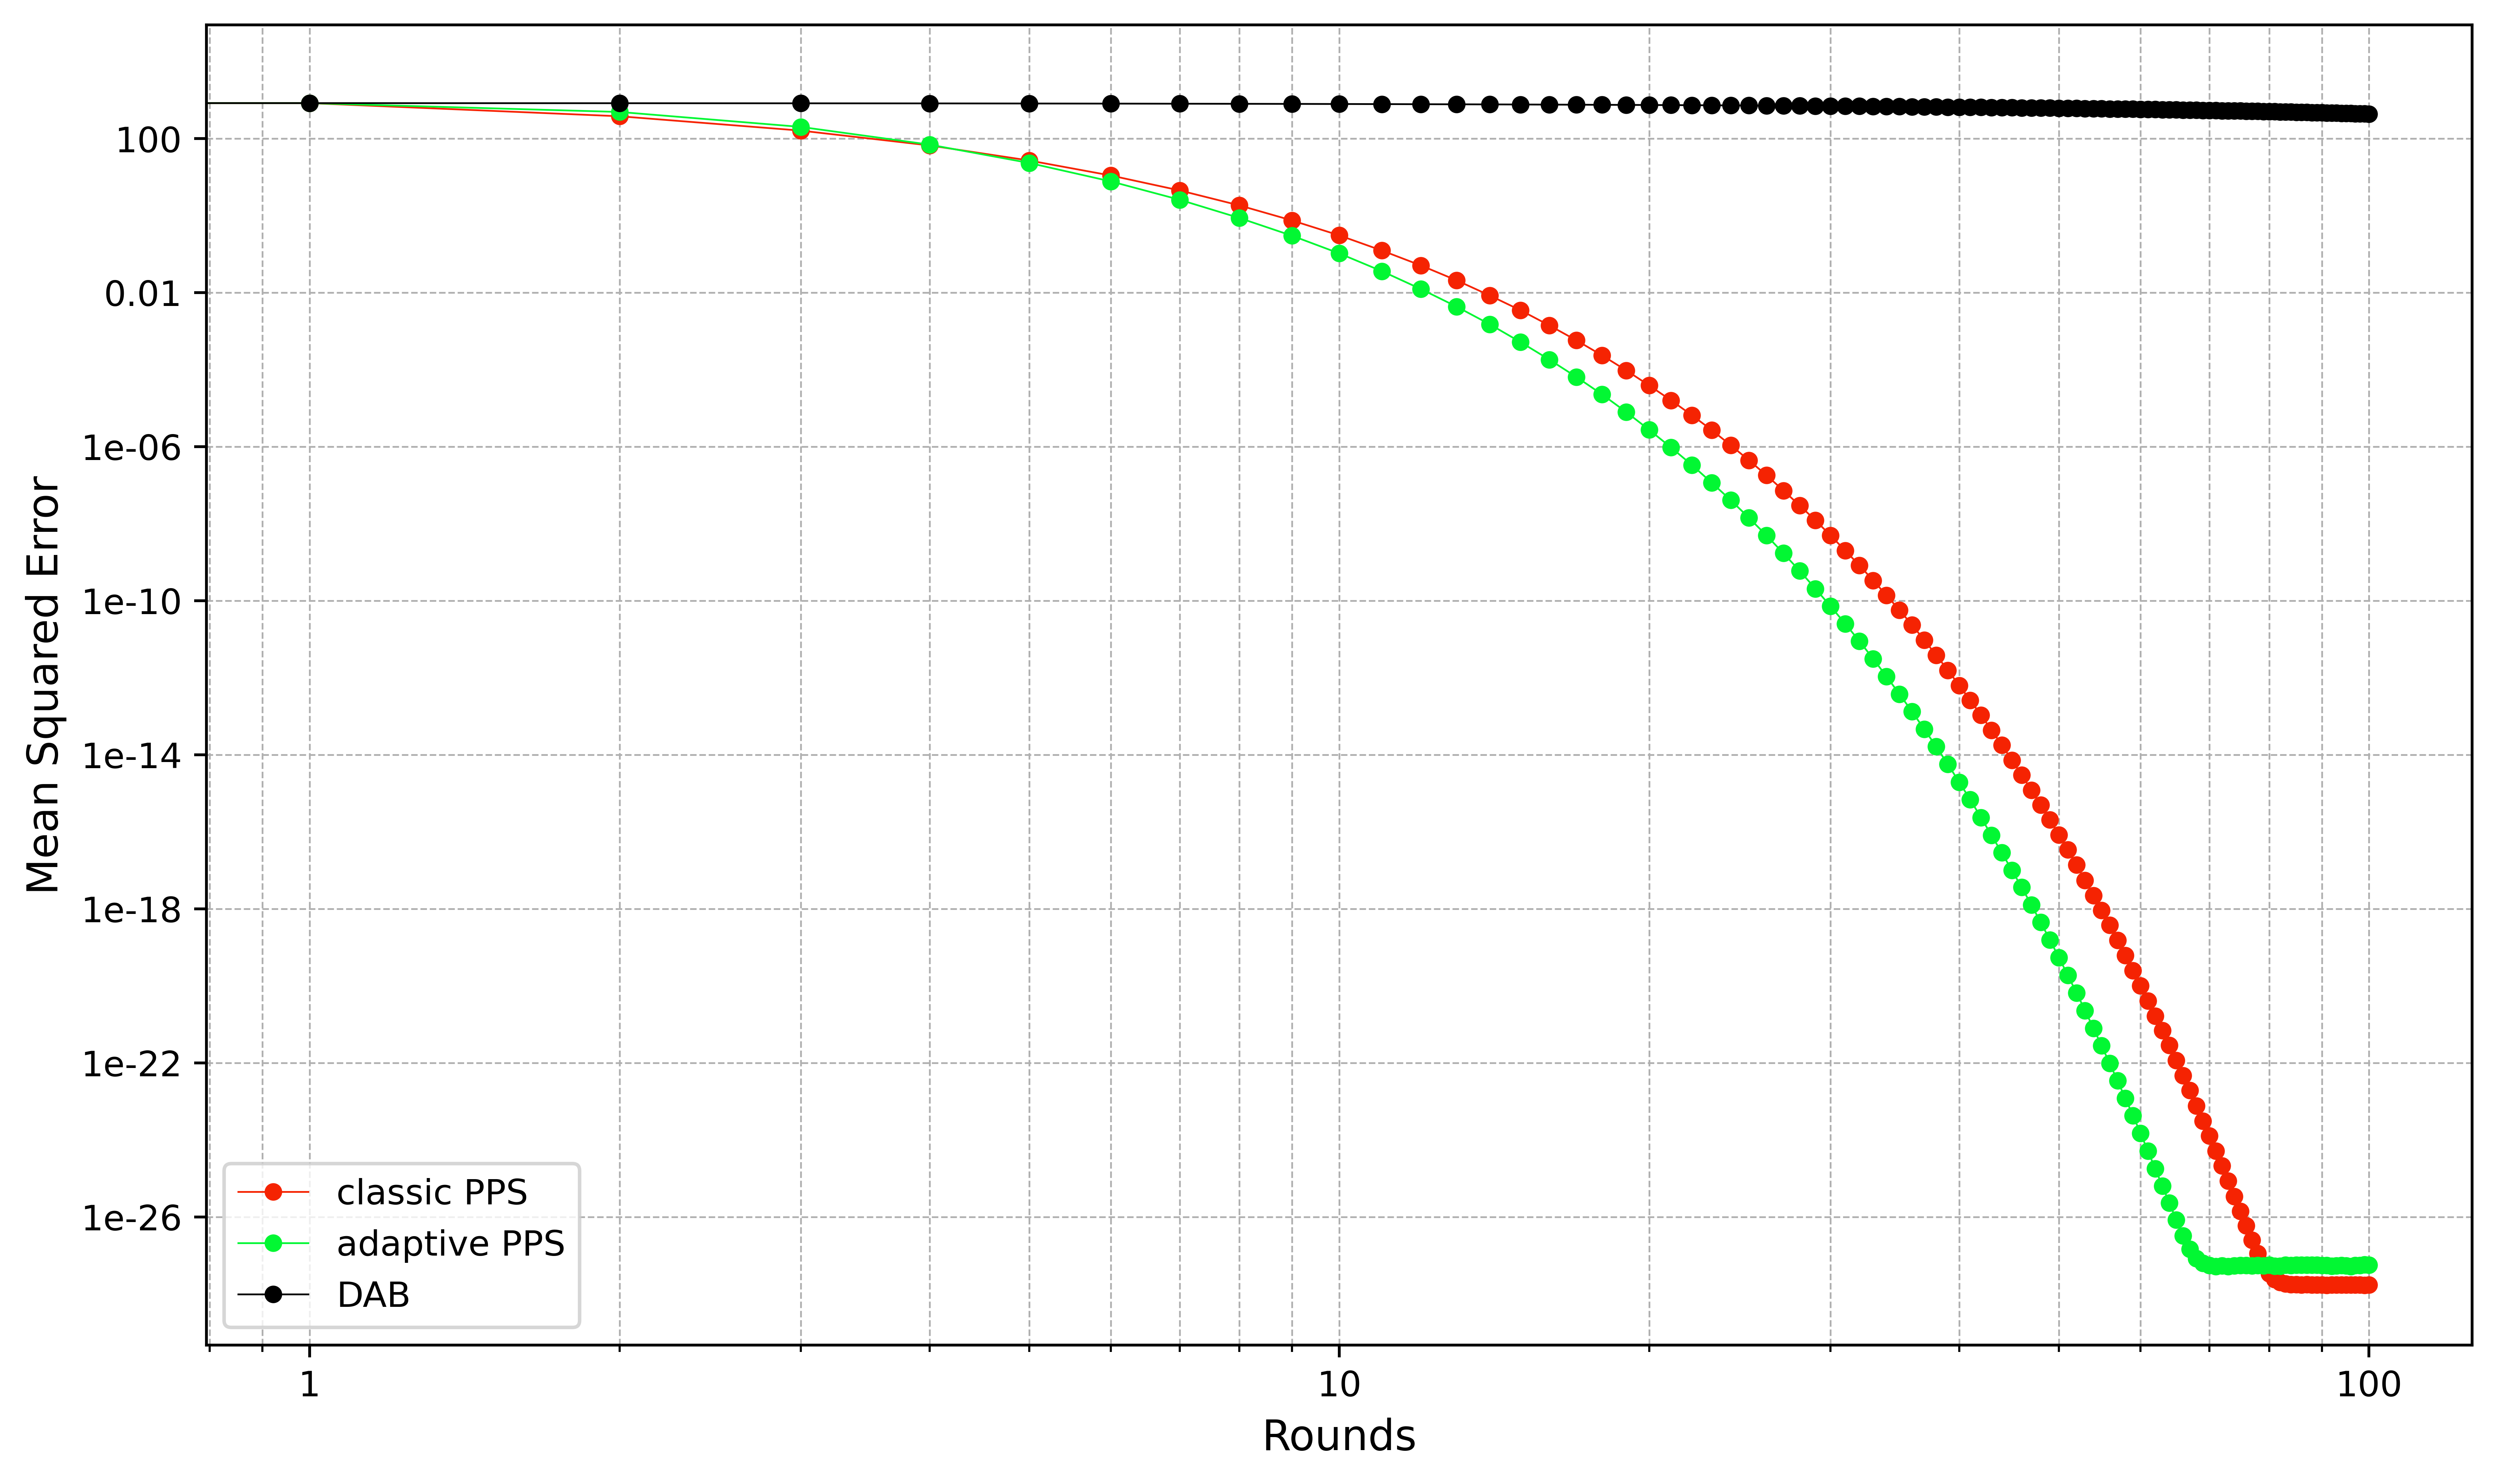
\includegraphics[width=\linewidth]{figures/Simulation_outcomes/CompleteGraph/DAB_vs_PPS_CG_r100_n1024_averaged_loglog.png}
    \caption{Complete graph: mean squared error per rounds (log-log)}
    \label{fig:completegraphMSEperRoundLogLog}
\end{figure}

Figure \ref{fig:completegraphMSEperRoundLogLog} presents the MSE reduction per round for the three load balancing algorithms simulated on the Complete graph on a log-log graph. The DAB curve (black curve) shows a linear trend and a gentle decrease of the MSE over the 100 rounds. The DAB performs poorly since it uses a fixed, deterministic load redistribution rule for its nodes, where each node selects the minimally loaded neighbor and proposes a load transfer. In a Complete graph where each node is interconnected, the same few nodes that hold the load of amount $L_{min}$ are the nodes that are receiving all the proposals. Since each minimal neighbor only accepts one proposal per round, the number of load transfers is heavily limited, resulting in slow MSE reduction. The PPS and ATPPS algorithms leverage the high connectivity of the network more effectively, due to their randomized nature. The PPS curve (red curve) exhibits a steady decrease in MSE, therefore showing efficient MSE reduction over time. Since all nodes are equally connected, no structural constraints slow down the process of pushing and pulling loads from neighbors. However, PPS does not distinguish between nodes that are highly imbalanced and those that are nearly balanced, leading to unnecessary load transfers in later rounds, which slows convergence. The ATPPS algorithm (green curve) achieves even faster MSE reduction than PPS. As the system nears equilibrium, ATPPS reduces redundant exchanges, causing the red curve to stagnate after a certain point in time. In summary, DAB underperforms due to limitations on the amount of load transfers; PPS improves upon this but lacks adaptive control, while ATPPS optimally balances load while avoiding unnecessary exchanges, making it the most effective approach in this setting.

Figure \ref{fig:dabCompleteModelFit} shows the exponential regression fit for the MSE data when the DAB algorithm as a load balancing algorithm is applied to the network. Even though the curve might not suggest an exponential decay, the MSE data fits with the exponential regression model following the equation $MSE_r=844.63*e^{-0.01*r}$. The decay rate of -0.01 suggests a very slow decrease in MSE. The fitted curve and model seem very suitable for the MSE data, since the fitted curve aligns with the MSE data. The MSE data of the PPS is fitted to the exponential regression model for rounds 10 to 80. Over time, repeated randomized exchanges smooth out load imbalances, leading to an exponential decay in MSE, as seen in figure \ref{fig:ppsCompleteModelFit}. The best fit follows the equation $MSE_r=2530.41*e^{-0.9*r}$. In Figure \ref{fig:atppsCompleteModelFit}, the exponential regression fit is visualized for the MSE data of the ATPPS load balancing algorithm graph in the complete graph for rounds 10 to 65. The fitted curve is expressed by the equation $MSE_r=4309.94*e^{-1.06*r}$. A steep error reduction is indicated by the decay rate of -1.06. As the PPS algorithm, the ATPPS algorithm reduces the error very effectively in an exponential manner. Rounds 66 to 100 show a plateauing of the MSE data. The adaptive mechanism provides a faster decline in error indicated by the decay rate of -1.06 versus the one of the PPS of -0.9.

Figure \ref{fig:completegrapslopes} visualizes a heat map of the slopes (rates of change) for the three load balancing algorithms across different regions of the graph. The values reflect how steeply the MSE decreases over rounds. PPS and ATPPS have steep negative slopes in the start region, rounds 1-10 with a value of -92, indicating rapid initial improvement. However, their slopes in the middle (rounds 11-65) and end regions (rounds 66-100) approach zero, suggesting a plateau in performance. DAB has shallower negative slopes overall, reflecting a more gradual and consistent error reduction across all regions. The general slopes (rounds 1-100) for PPS and ATPPS (-8.4) are much steeper than DAB (-4.4), suggesting that PPS and ATPPS converge faster on average. The end region is chosen as 66-100 to catch the trend of plateauing for the ATPPS and also for PPS, which is beginning to plateau in error reduction in later rounds (rounds 80-100). The MSE is reduced significantly by the PPS and ATPPS. The initial MSE value of $832$ is reduced to $1.72 \times 10^{-28}$ for the PPS and $5.63 \times 10^{-28}$ for the ATPPS, while the DAB reduced the error to nearly half of the initial value, achieving a value of $436.84$.

\begin{figure}[]
    \centering
    \scalebox{0.8}{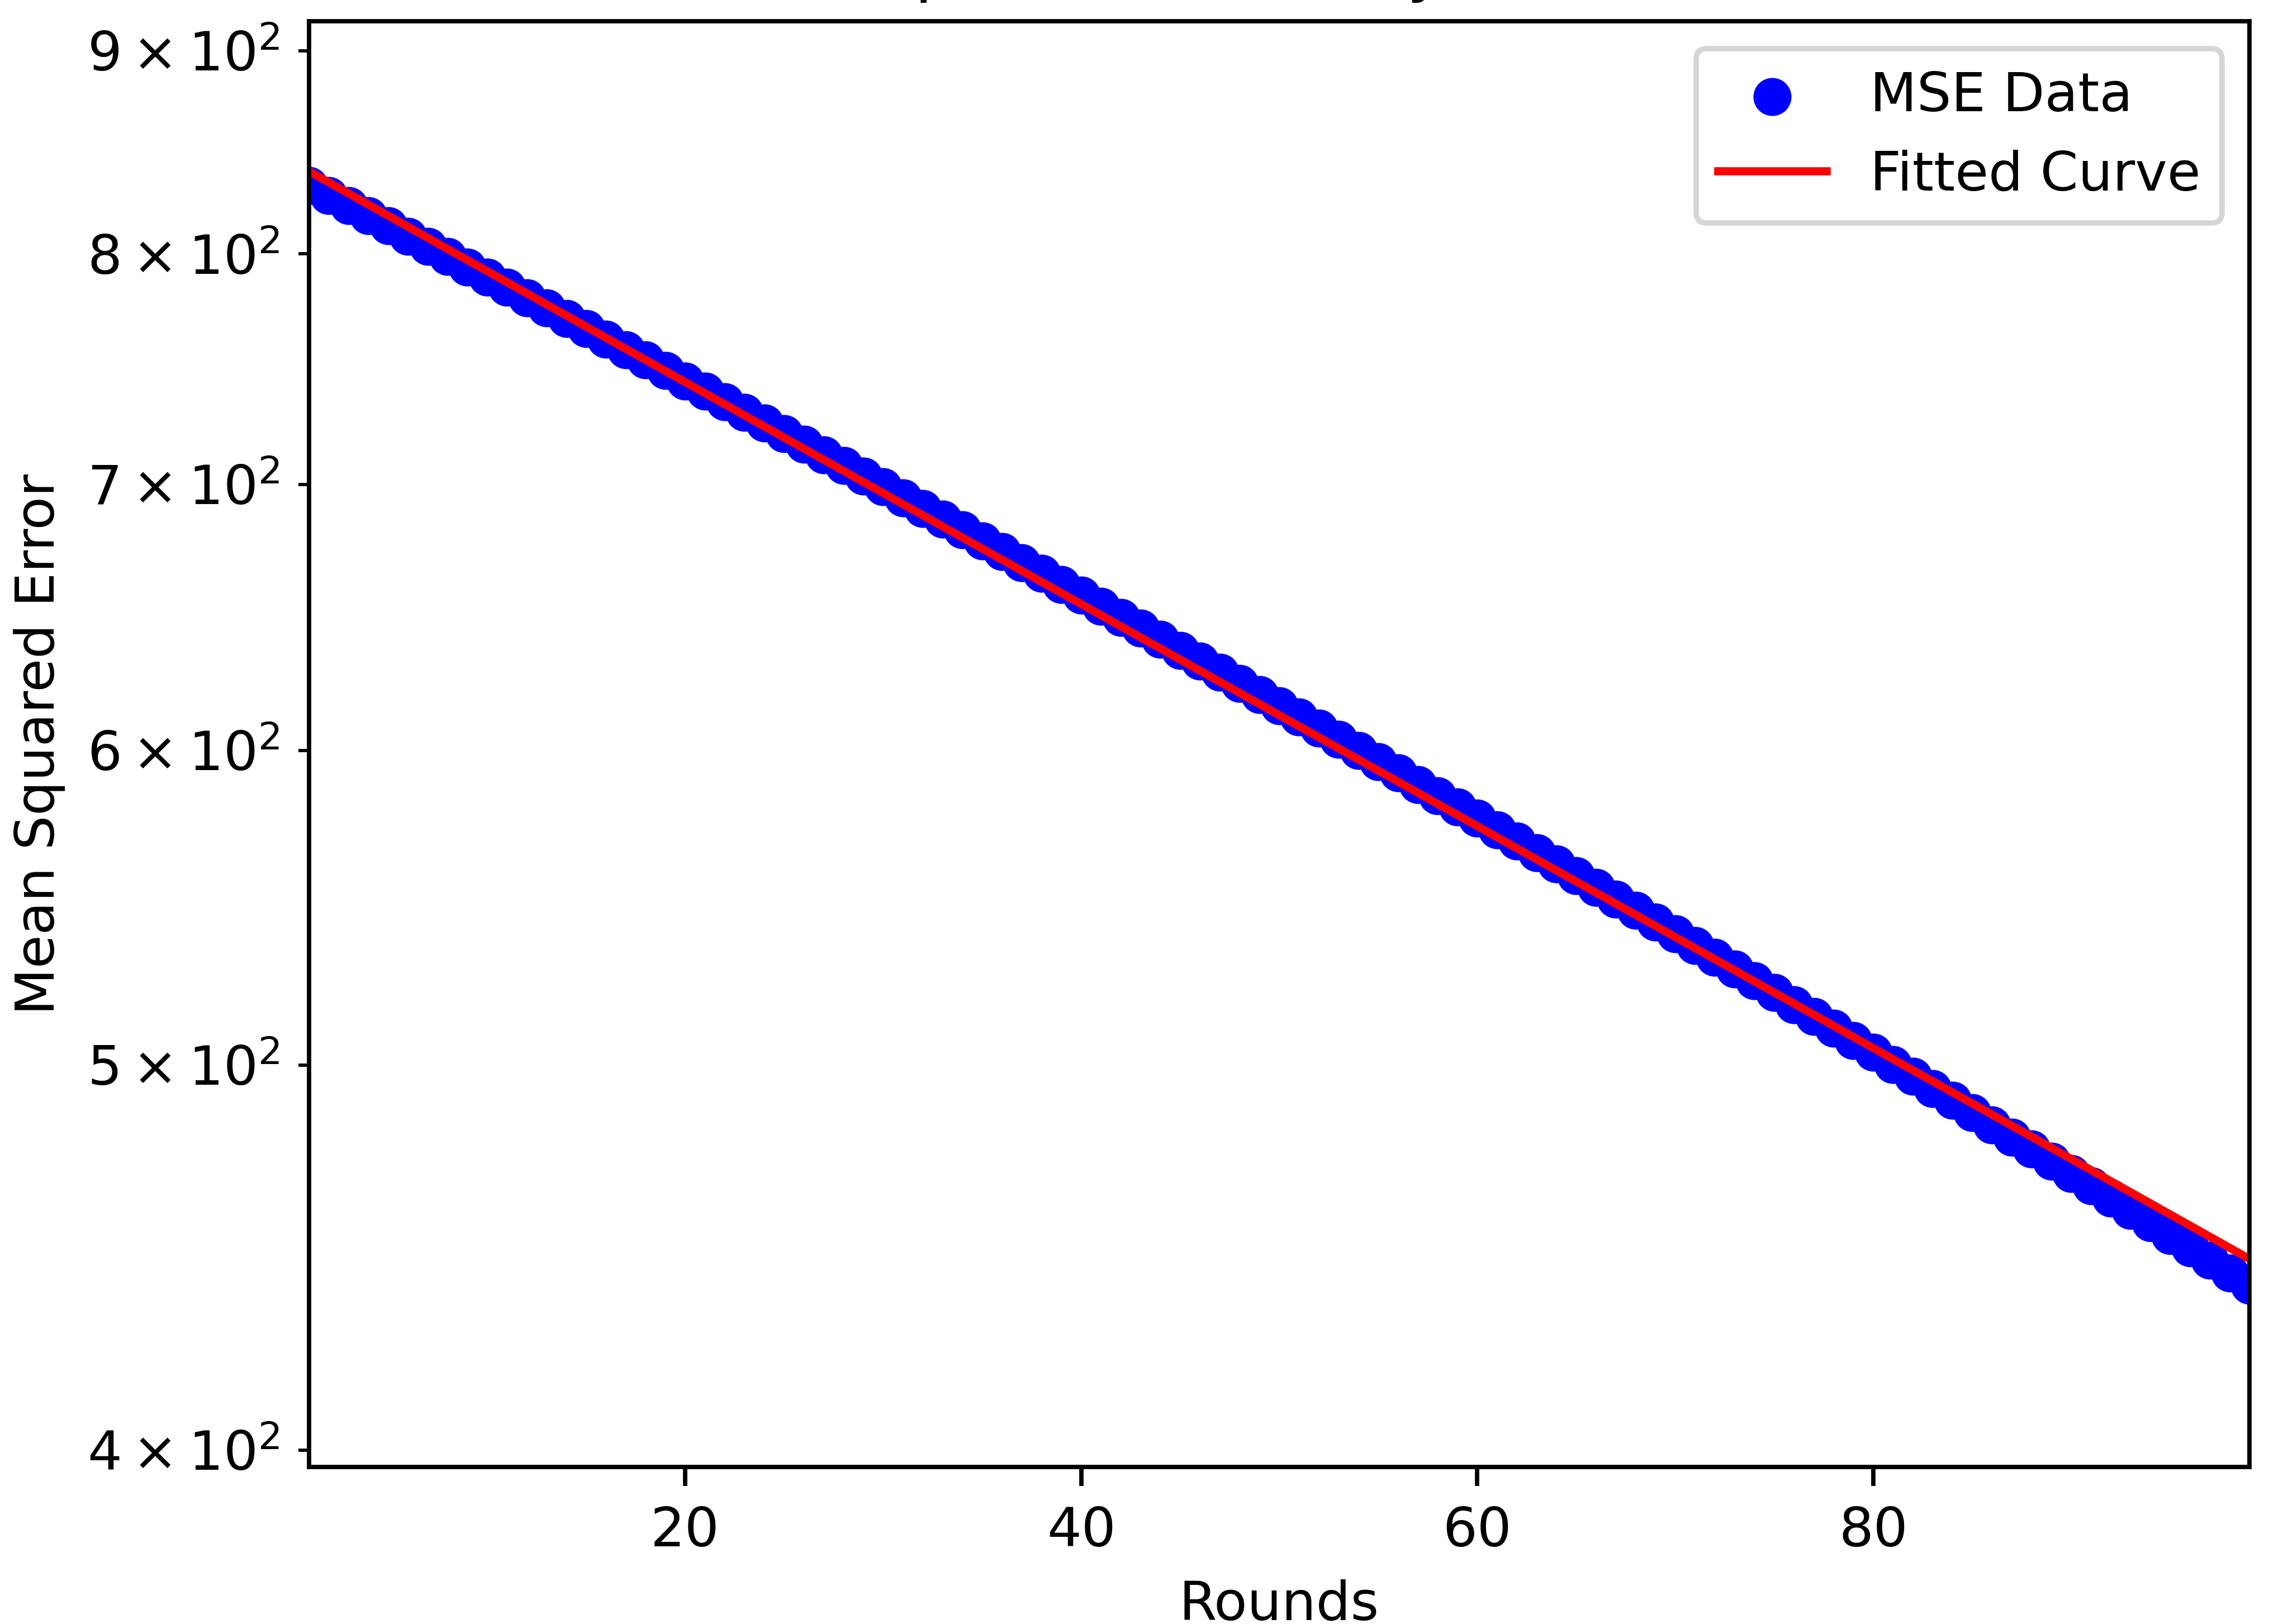
\includegraphics{figures/Simulation_outcomes/CompleteGraph/DAB/DAB_modelfitting_rounds_99_model_1.png}}
    \caption{Complete graph - exponential regression fit: DAB}
    \label{fig:dabCompleteModelFit}
\end{figure}

\begin{figure}[]
    \centering
    \scalebox{0.8}{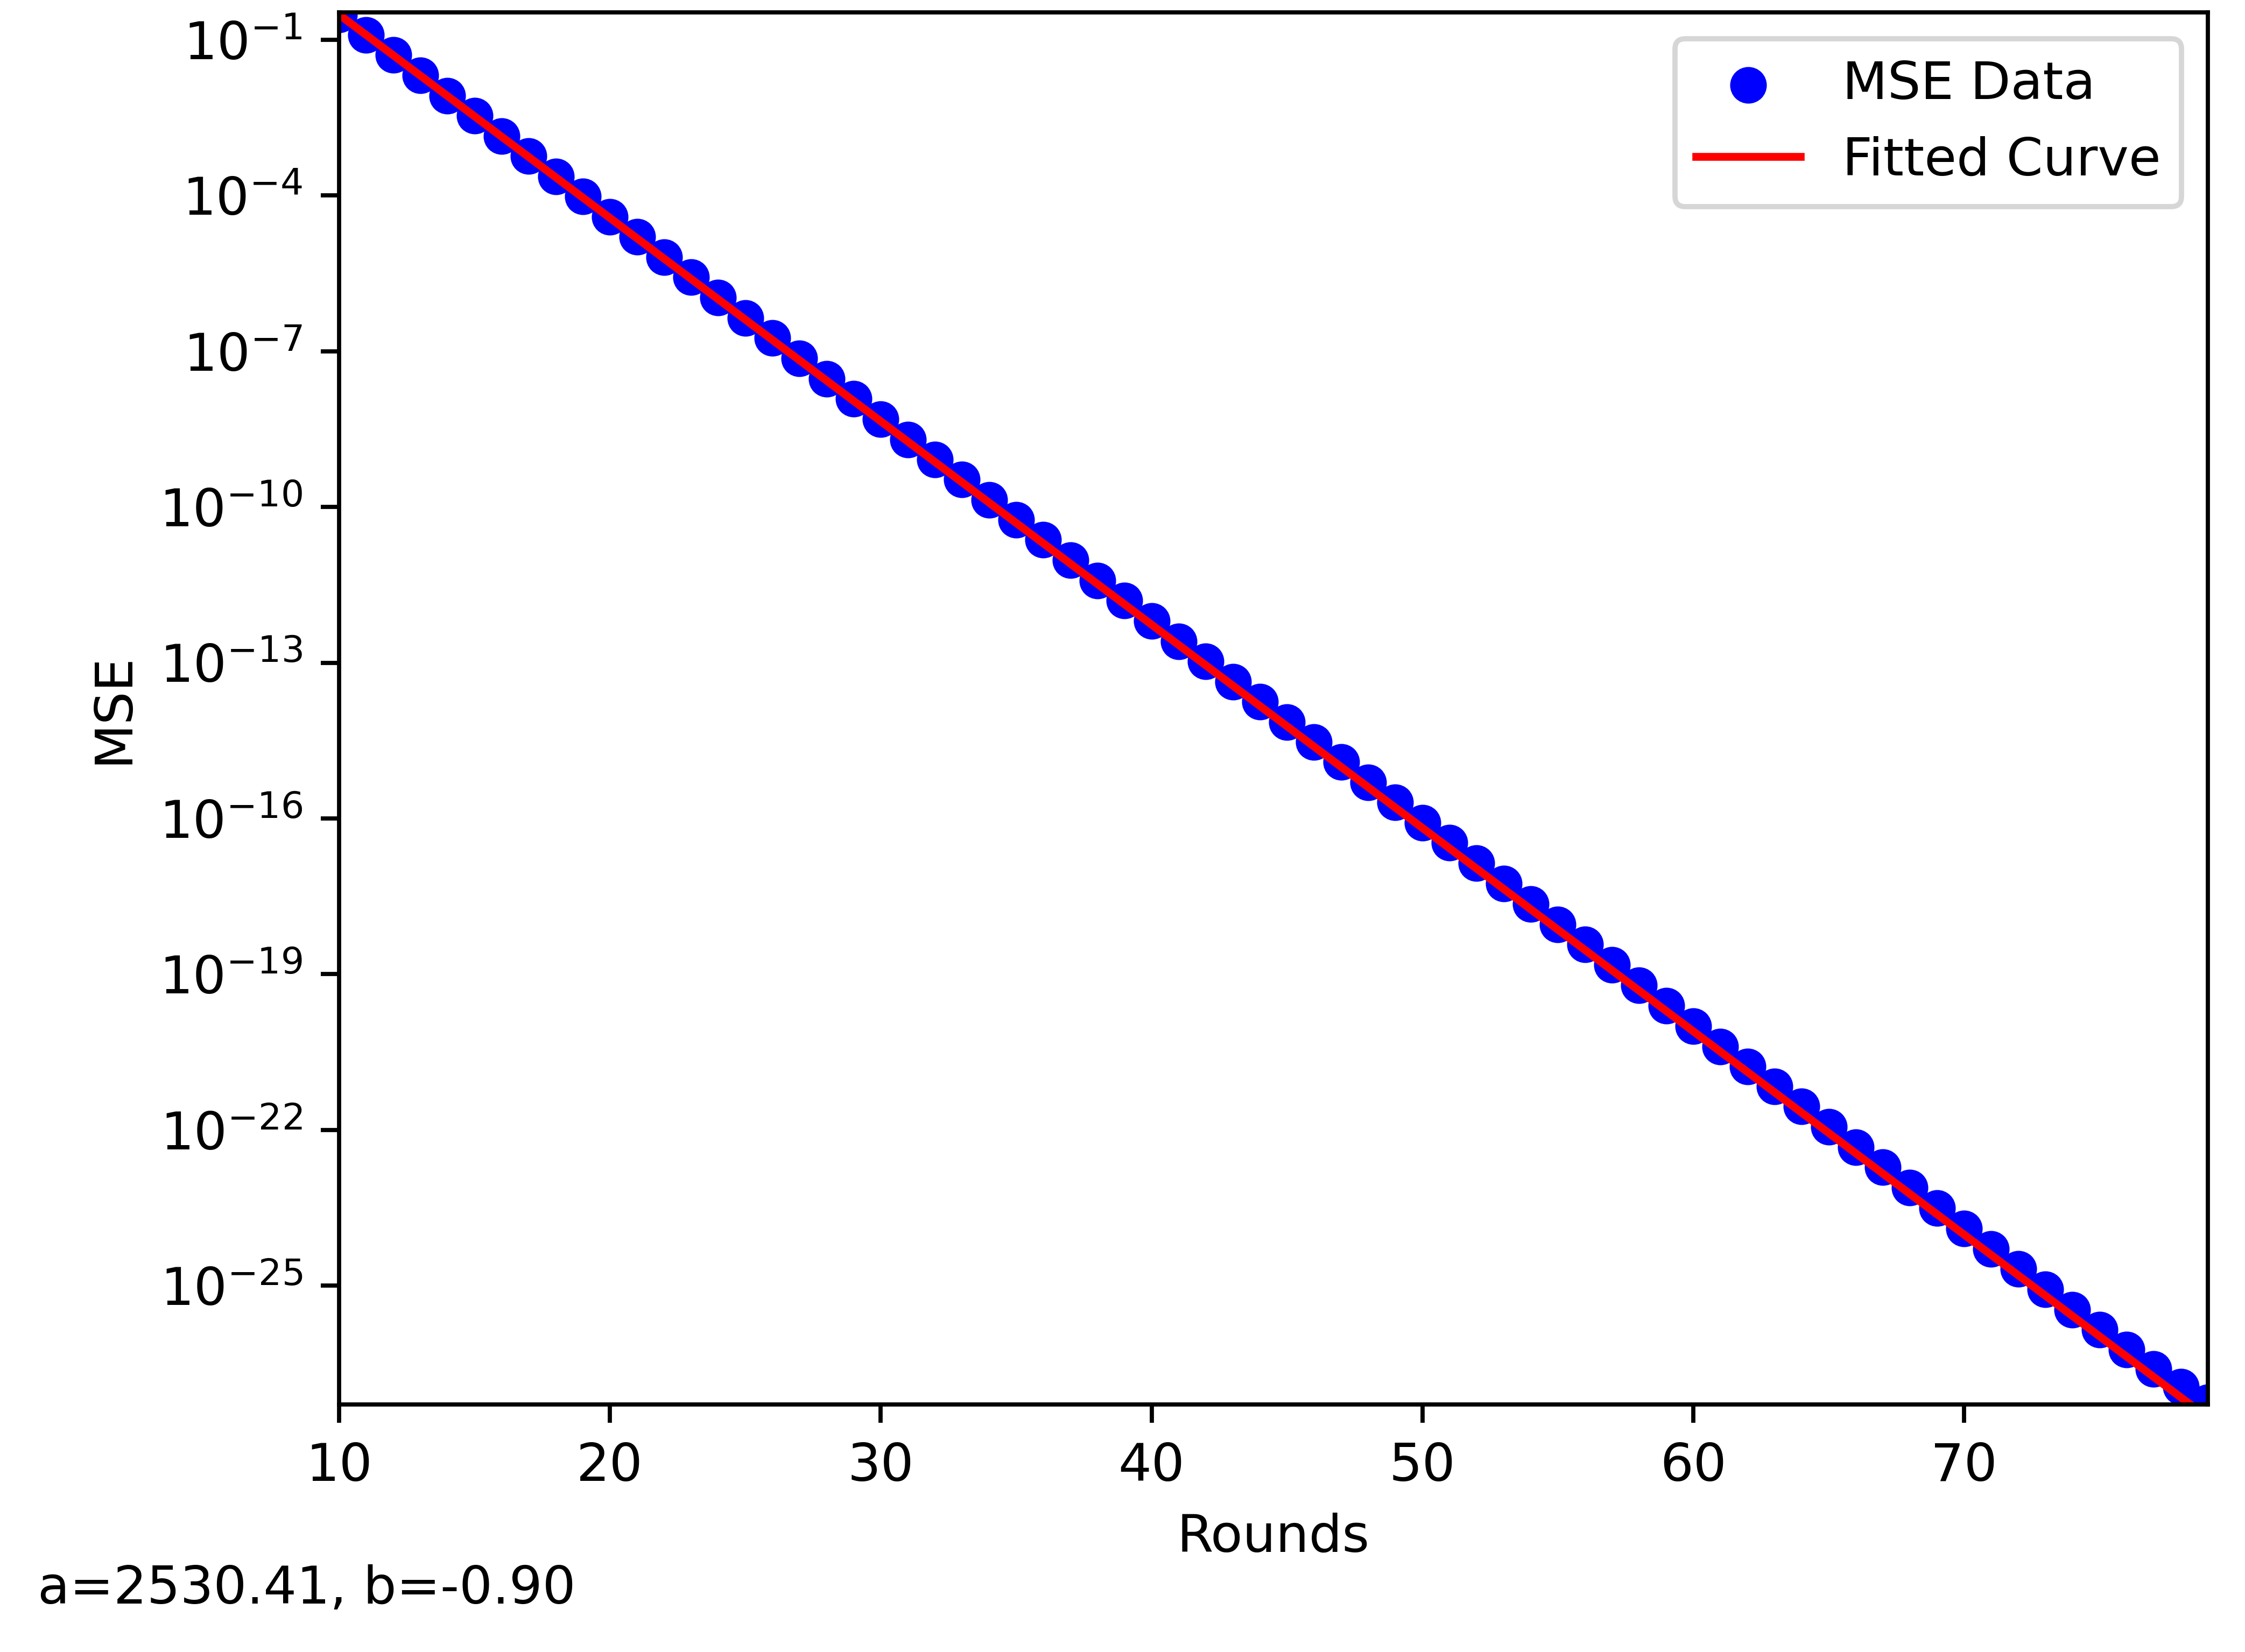
\includegraphics{figures/Simulation_outcomes/CompleteGraph/PPS/PPS_modelfitting_rounds_79_model_1.png}}
    \caption{Complete graph - exponential regression fit: PPS}
    \label{fig:ppsCompleteModelFit}
\end{figure}

\begin{figure}[]
    \centering
    \scalebox{0.8}{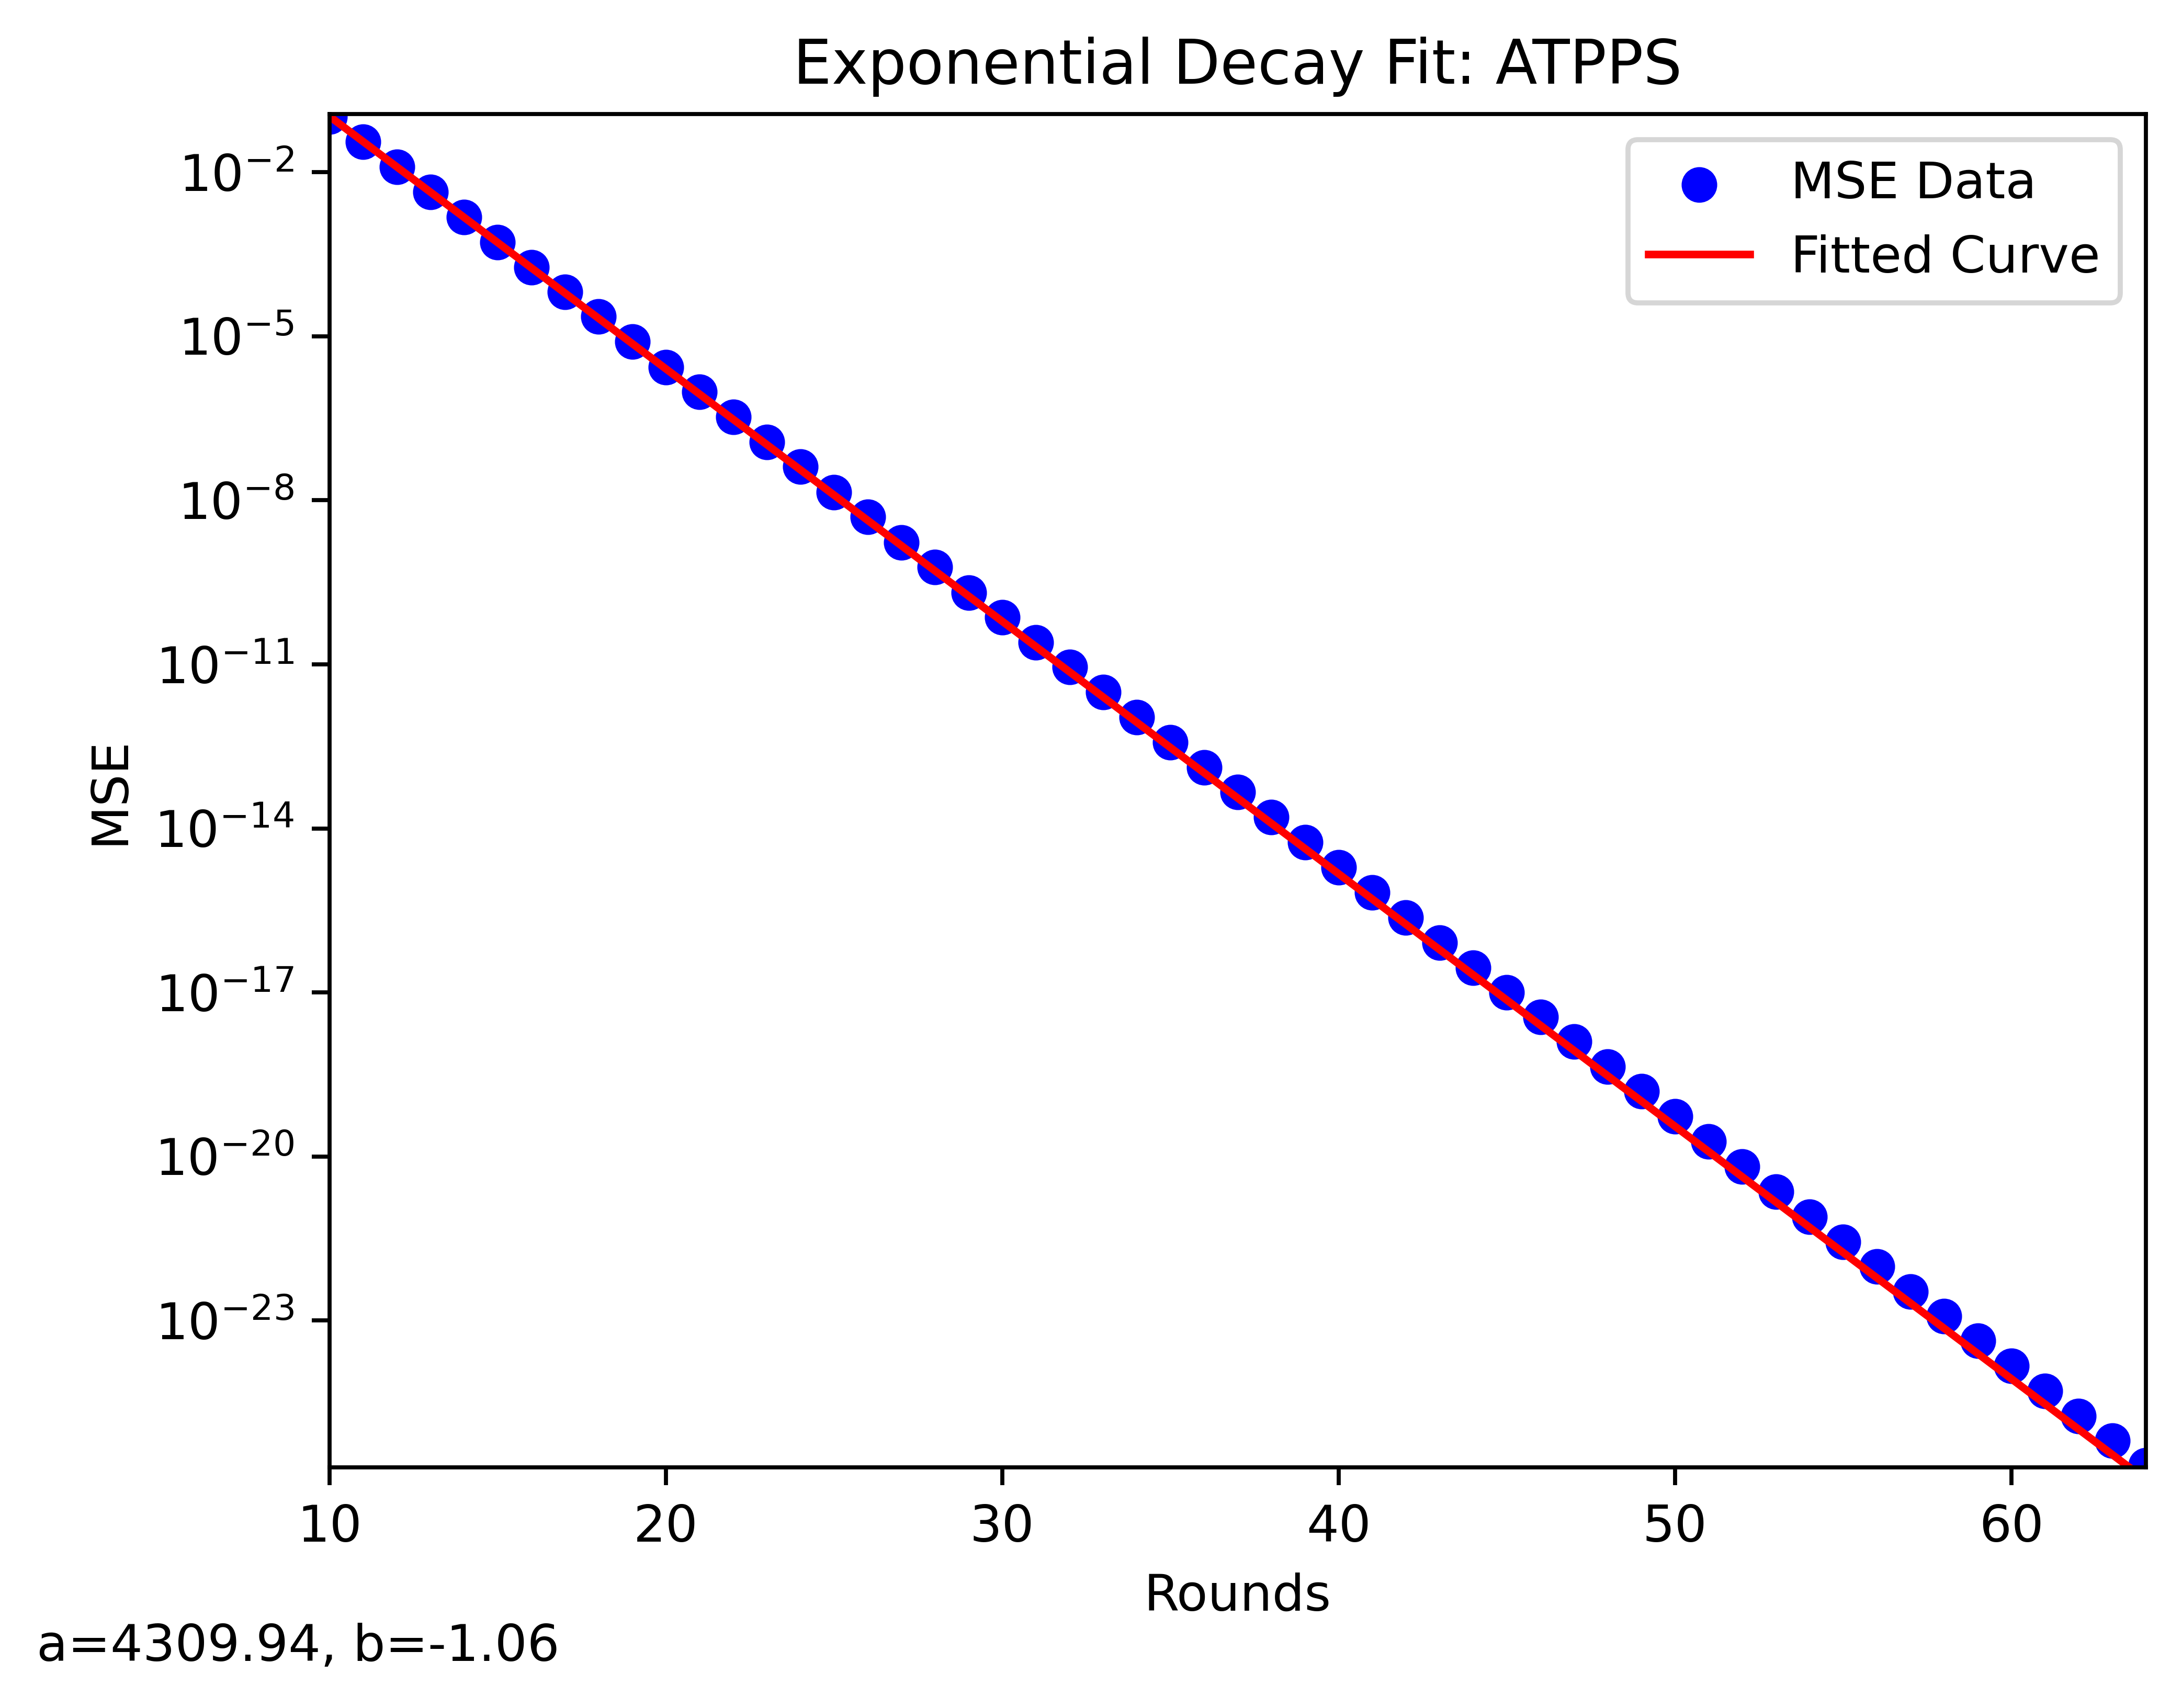
\includegraphics{figures/Simulation_outcomes/CompleteGraph/ATPPS/ATPPS_modelfitting_rounds_64_model_1.png}}
    \caption{Complete graph - exponential regression fit: ATPPS}
    \label{fig:atppsCompleteModelFit}
\end{figure}

\begin{figure}
    \centering
    \scalebox{0.8}{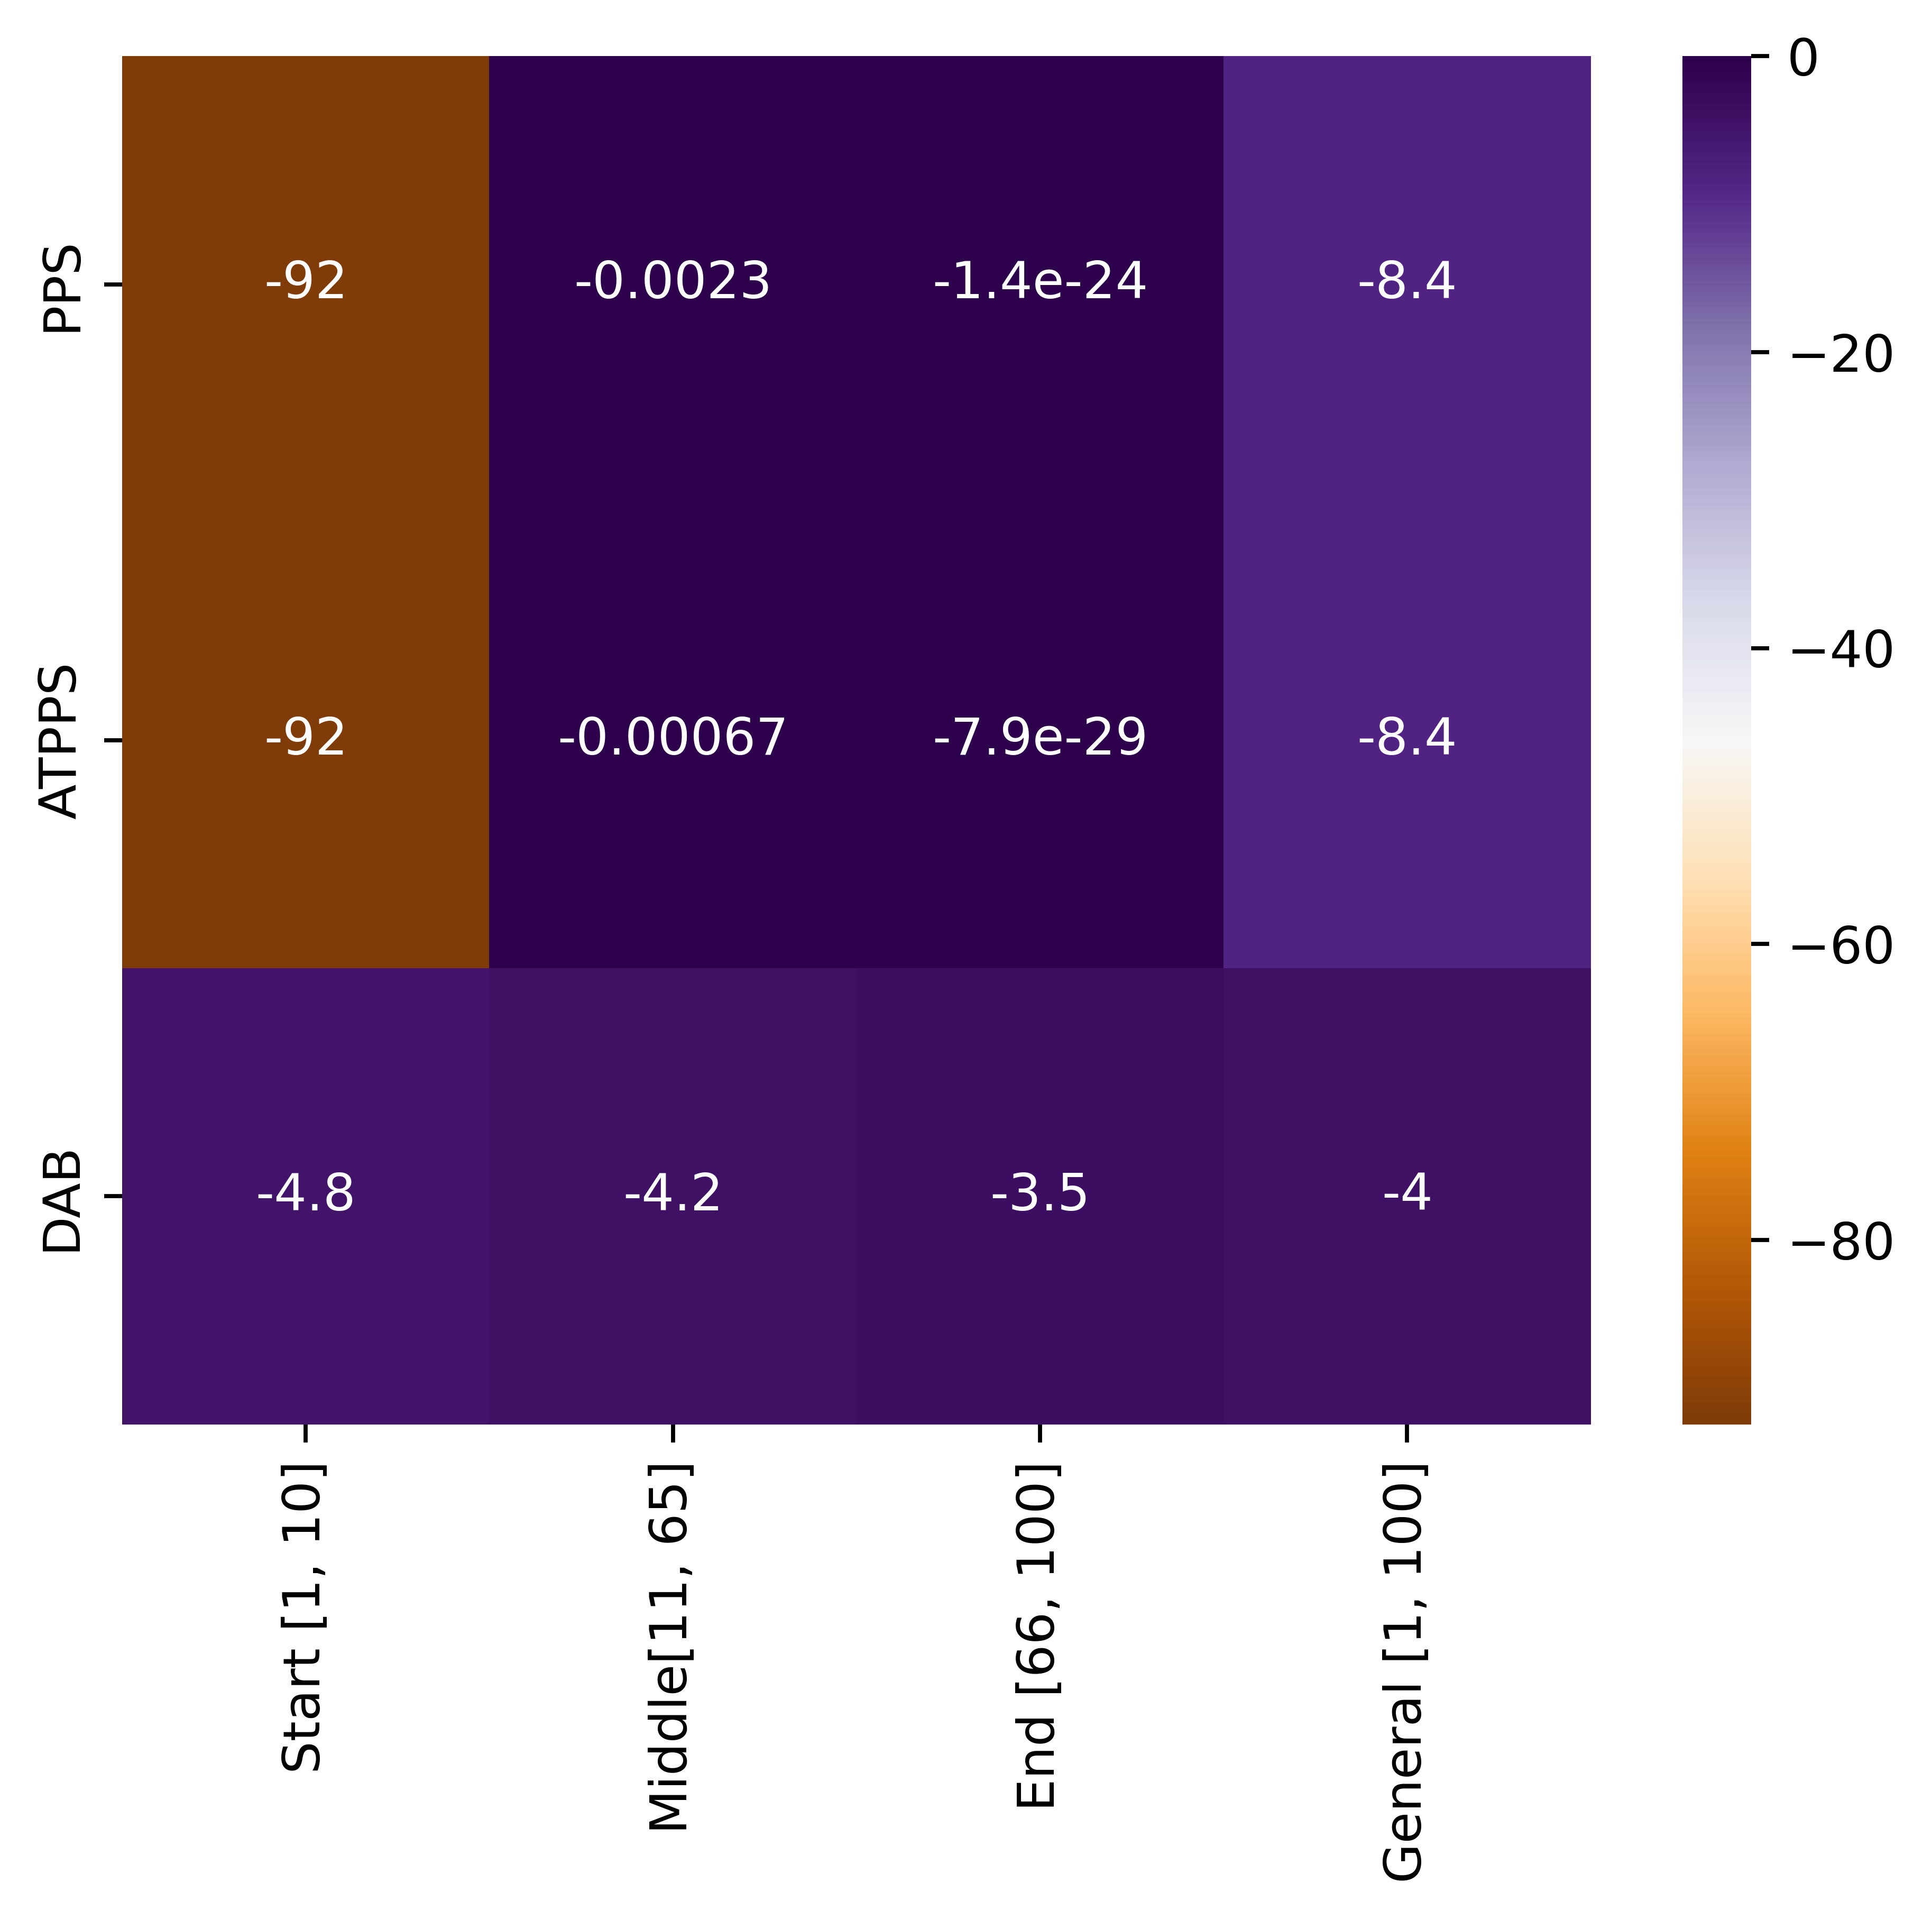
\includegraphics{figures/Simulation_outcomes/CompleteGraph/DAB_vs_PPS_vs_ATPPS_slopesheatmap_100rounds.png}}
    \caption{Complete graph: heat map of slopes per region}
    \label{fig:completegrapslopes}
\end{figure}

\section{Star Graph}\label{sec:stargraph}
The behavior of the curves in figure \ref{fig:stargraphMSEperRoundLogLog} is similar to those for the Complete graph, with the difference that the PPS curve falls more steeply than the ATPPS curve. Again, DAB shows a much slower MSE reduction compared to PPS and ATPPS, as indicated by the flatter slope of its curve. It converges minimally, with MSE remaining nearly constant over rounds after an initial reduction. This indicates that DAB is less efficient in balancing load in a Star graph, likely due to its deterministic nature and lack of dynamic adaptability. In the Star graph, all the leaves have the central node as a partner, meaning each leaf node selects the same central node to propose load transfers. When the central node has a higher load than the leaf requesting a transfer, no load transfer occurs between these two nodes, creating a bottleneck. Both PPS and ATPPS exhibit steep MSE reductions early on, as seen in the sharp downward trends in the log-log plot. The PPS algorithm balances load more efficiently than the ATPPS algorithm since it reduces MSE faster and reaches lower MSE values sooner (as of round 45) before the curve plateaus. The Push-Pull Sum based algorithms draw an advantage from the Star graph, as the redistribution happens through the central node, which is chosen by every leaf node as a push destination. Following that, the central node redistributes parts of the load to the leaf nodes in magnitude of $\frac{\frac{s_i,r}{2}}{N-1}$.

As seen in figure \ref{fig:dabStarModelFit} the MSE data for the DAB-balanced network aligns nearly perfectly with the fitted curve of the exponential regression model given by the equation $MSE_r=840.42*e^{-0.01*r}$ for the rounds 1 to 100, even though the decay rate of -0.01 indicates a very slow reduction in error. From round to round, the improvement in the network remains minimal. This highlights the inability of the DAB to balance the network within 100 rounds to a satisfactory level. Figures \ref{fig:ppsStarModelFit} and \ref{fig:atppsStarModelFit} show the fitted curves for the MSE data of the PPS and ATPPS algorithms, respectively. The best-fit model for the MSE data of the PPS load balancing algorithm between rounds 10 to 45 follows the equation $MSE_r=29794.60*e^{-1.39*r}$. The rounds 10 to 45 exhibit the steepest decline in MSE, and for that reason, they have been fitted to an exponential regression model. The decay rate of $-1.39$ indicates a rapid reduction in error, especially in comparison to DAB. For the ATPPS algorithm, the MSE data fits best with the exponential model in the range of rounds 18 to 60, following the equation $MSE_r=9329.40*e^{-1.05*r}$. In Star graphs, the central node dominates communication, and load balancing heavily depends on that node. Threshold-based adjustments do not significantly impact performance under these conditions. The discrepancy between the two PPS algorithms can be explained by the fact that the ATPPS limits the number of messages due to the conditional threshold-based load transfer, which means that there is less interaction compared to the PPS.

Overall, the situation is similar to the Complete graph, with the Push-Pull Sum-based algorithms performing an extremely quick error reduction and the DAB reducing the error exponentially at a very slow rate. This behavior is captured in the heat map of figure \ref{fig:stargraphslopes}. While the DAB algorithm reduces the error with an average slope of $-3.75 \pm 0.55$ for the three regions, the Push-Pull Sum-based algorithms achieve an initial error reduction of approximately $-92$ within the first 10 rounds. The slopes approach zero in the middle and end regions, which implies negligible MSE reduction in later stages. This is because the network is already sufficiently balanced that later rounds will not see a noticeable improvement in the MSE. Both algorithms converge early and maintain a near-steady state afterward. The DAB's lack of adaptability leads to slower convergence and less effective load balancing, as reflected in its consistently shallow slopes. The MSE decreases from an initial value of $832$ to approximately $480.47$ for the DAB, while for the PPS and ATPPS algorithms, the MSE reaches values of $8.3\times 10^{-24}$ for the PPS and $\sim6.5 \times 10^{-24}$ for the ATPPS.

\begin{figure}[]
    \centering
    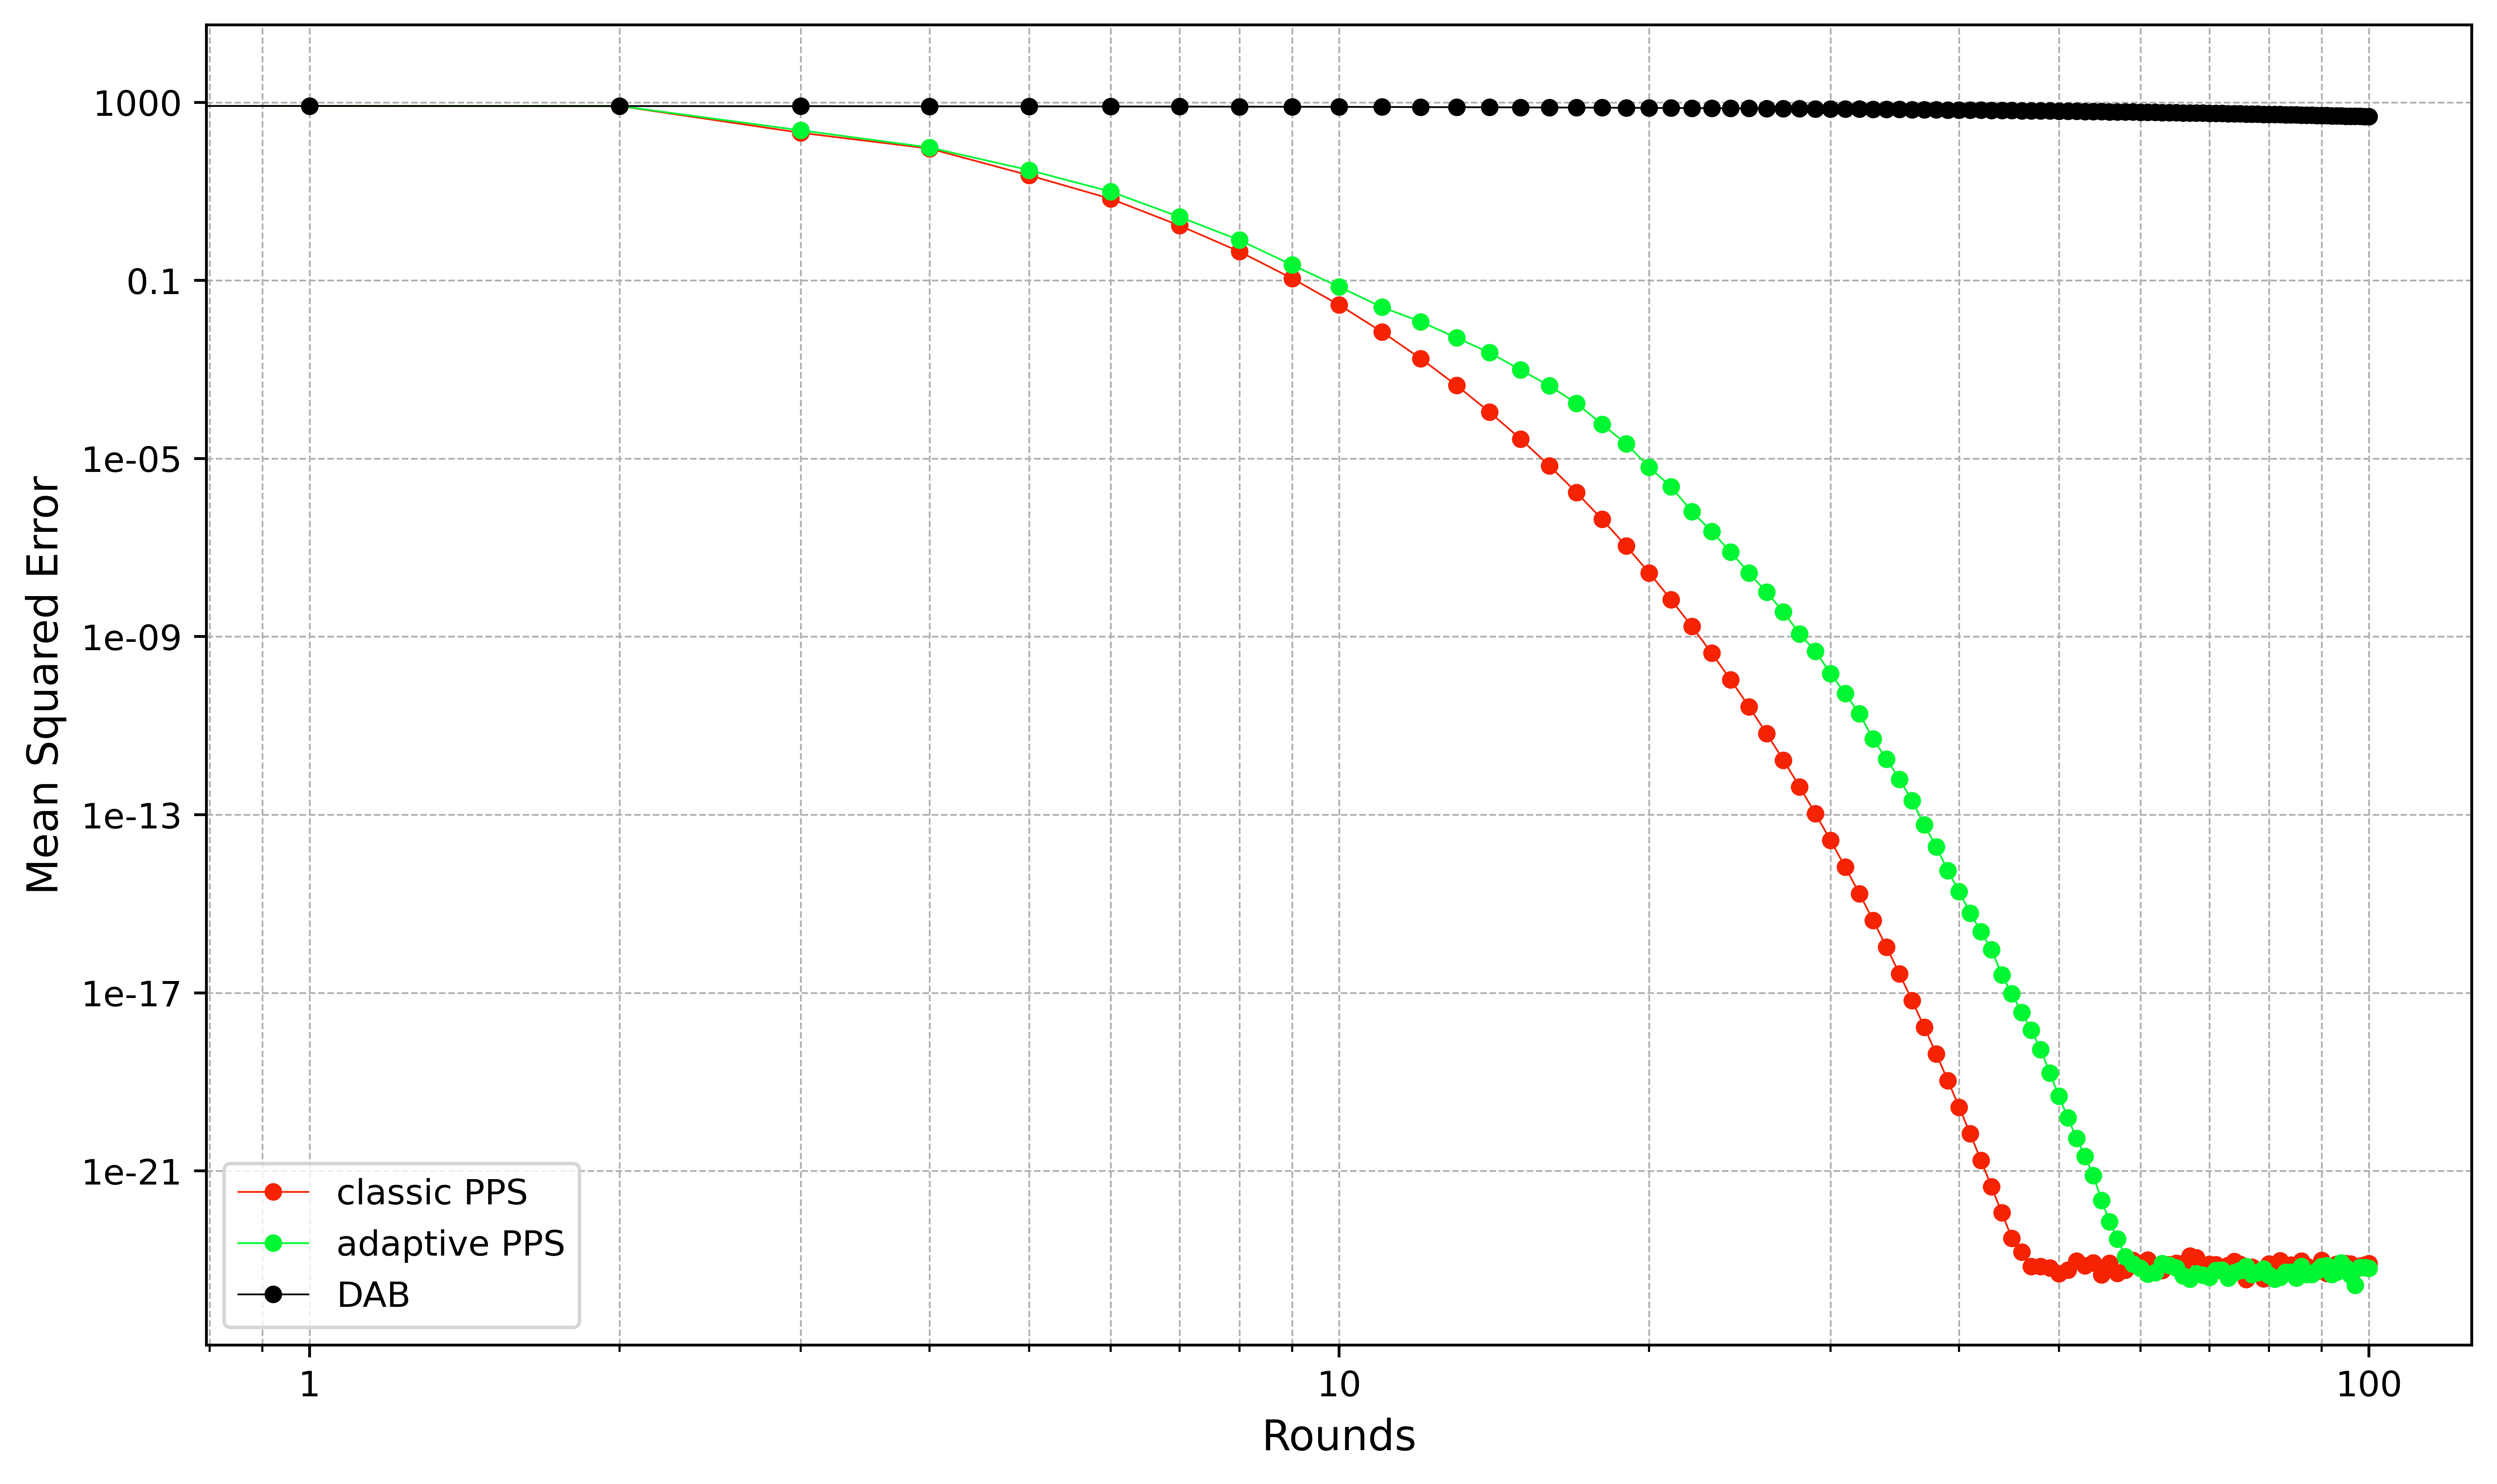
\includegraphics[width=\textwidth]{figures/Simulation_outcomes/StarGraph/DAB_vs_PPS_SG_r100_n1024_averaged_loglog.png}
    \caption{Star graph: mean squared error per rounds (log-log)}
    \label{fig:stargraphMSEperRoundLogLog}
\end{figure}
\begin{figure}[]
    \centering
    \scalebox{0.8}{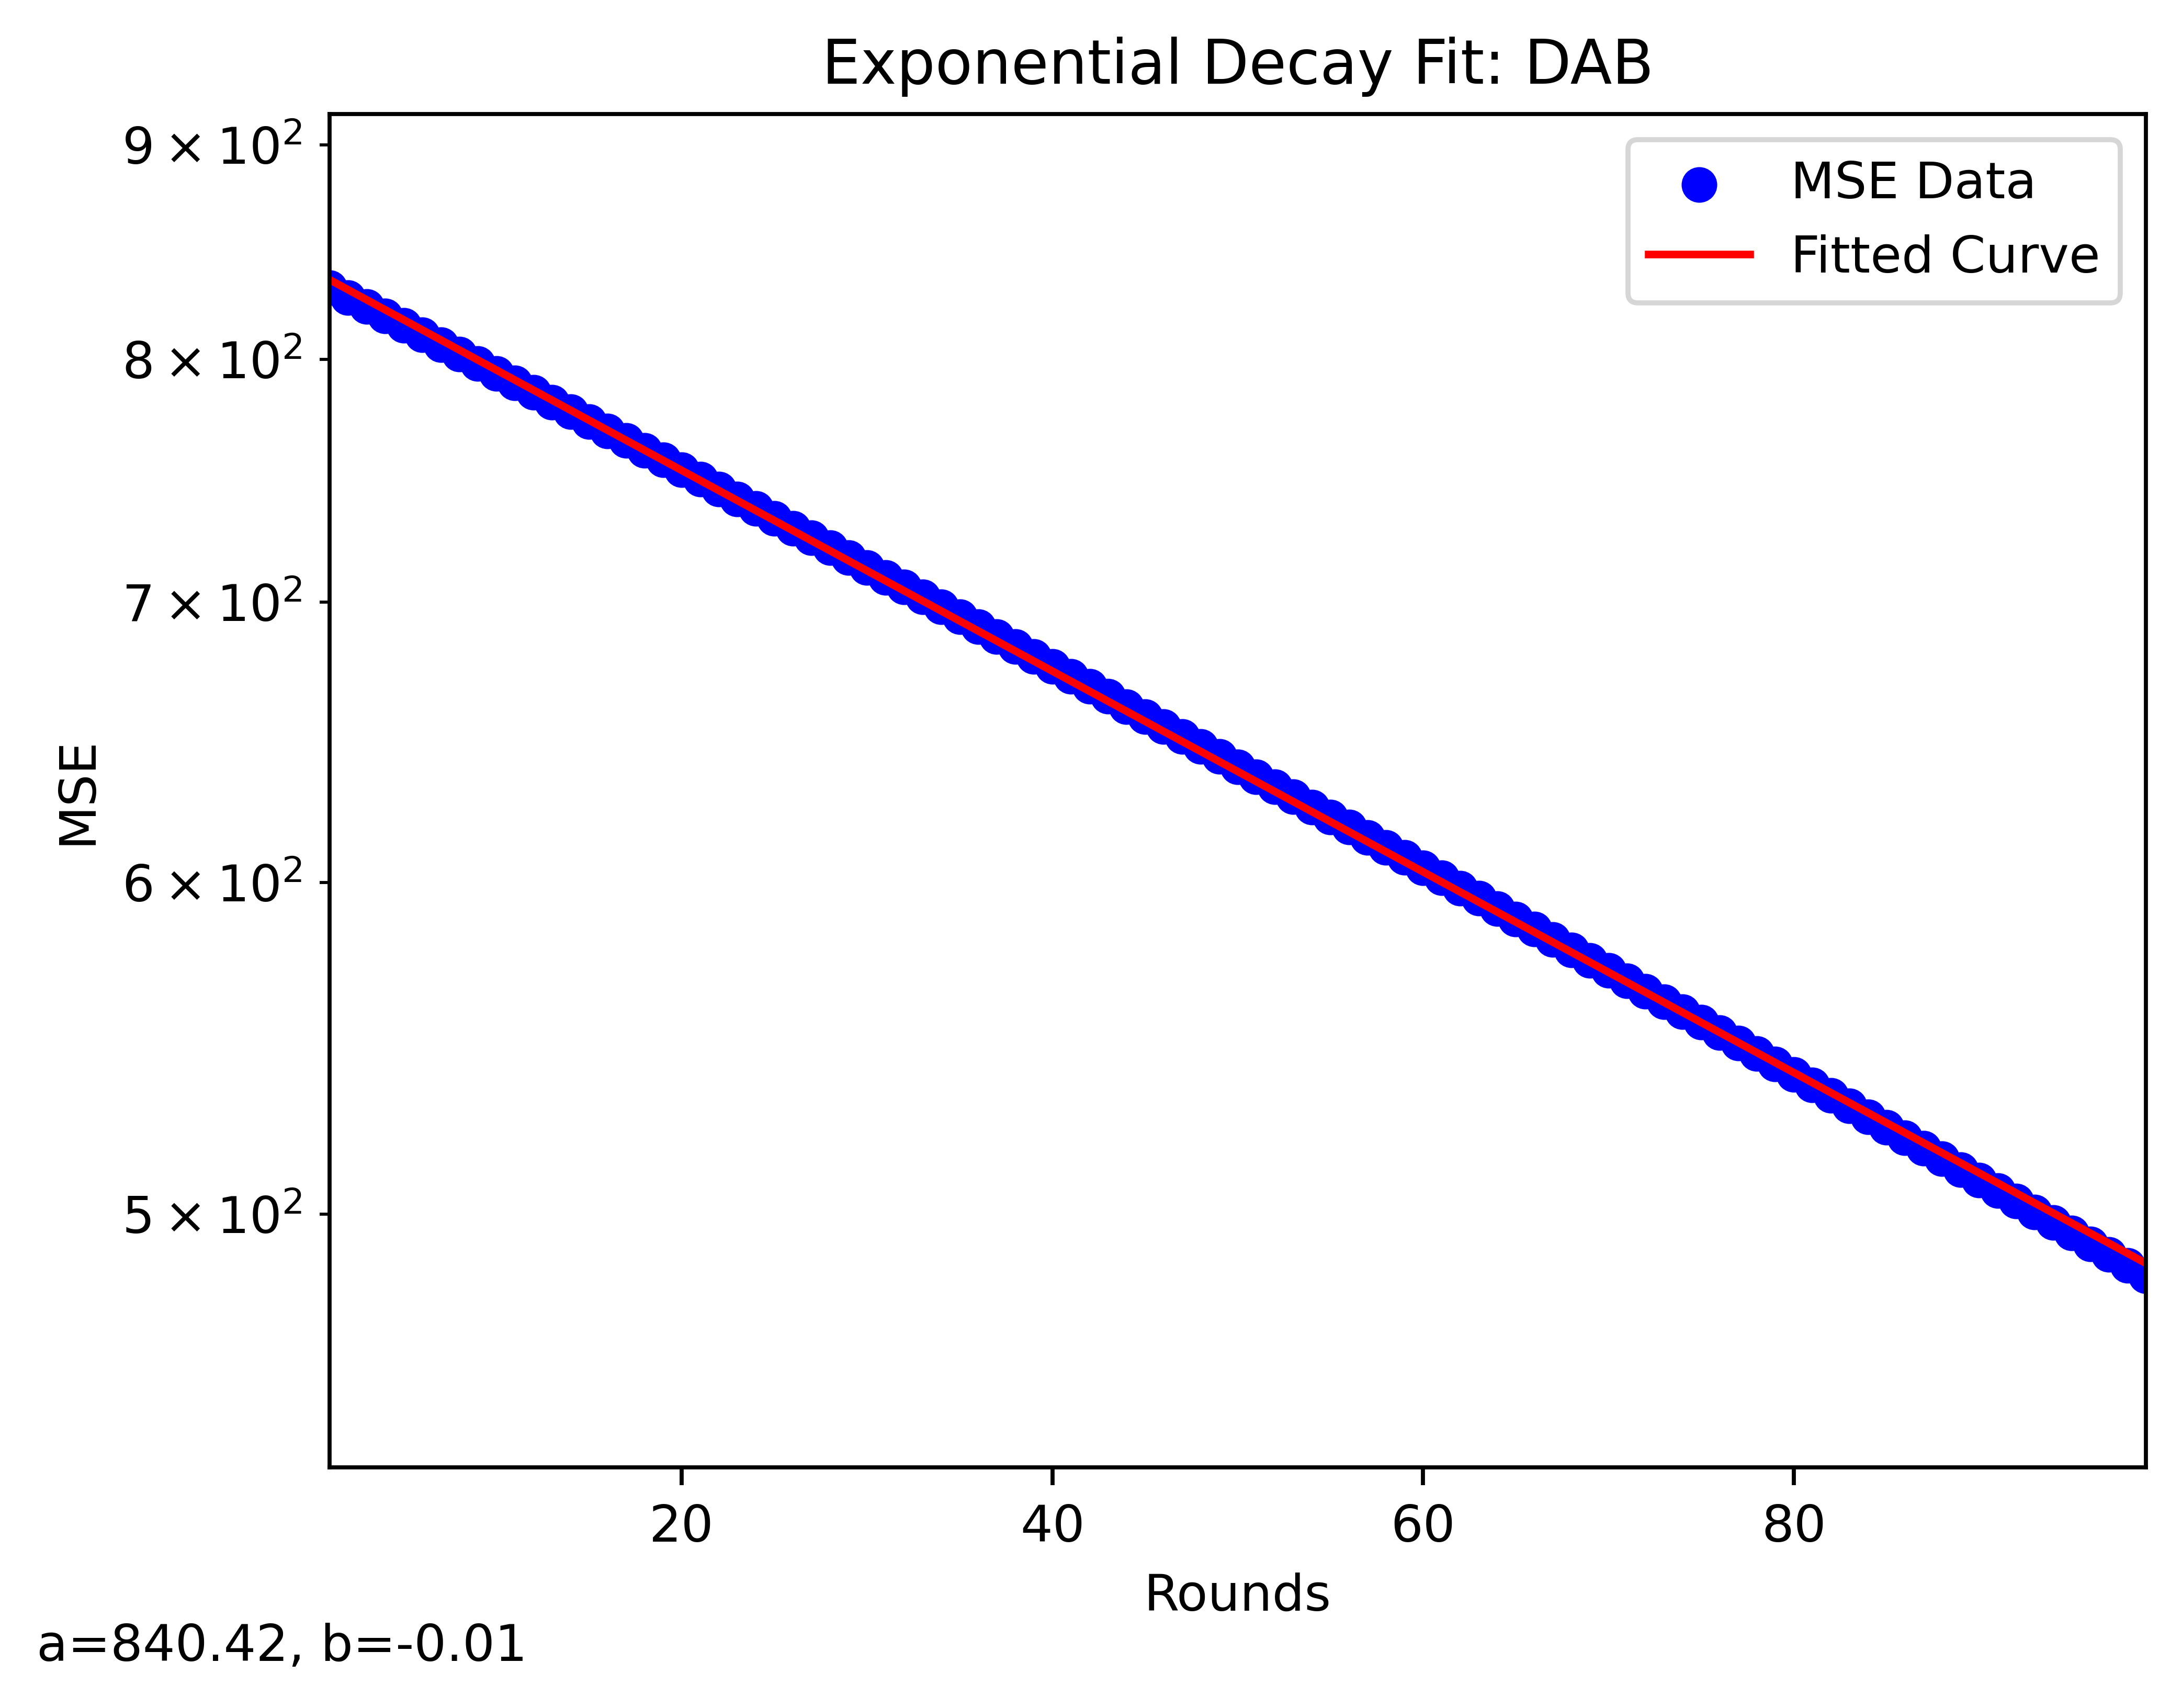
\includegraphics{figures/Simulation_outcomes/StarGraph/DAB/DAB_modelfitting_rounds_99_model_1.png}}
    \caption{Star graph - exponential regression fit: DAB}
    \label{fig:dabStarModelFit}
\end{figure}
\begin{figure}[]
    \centering
    \scalebox{0.8}{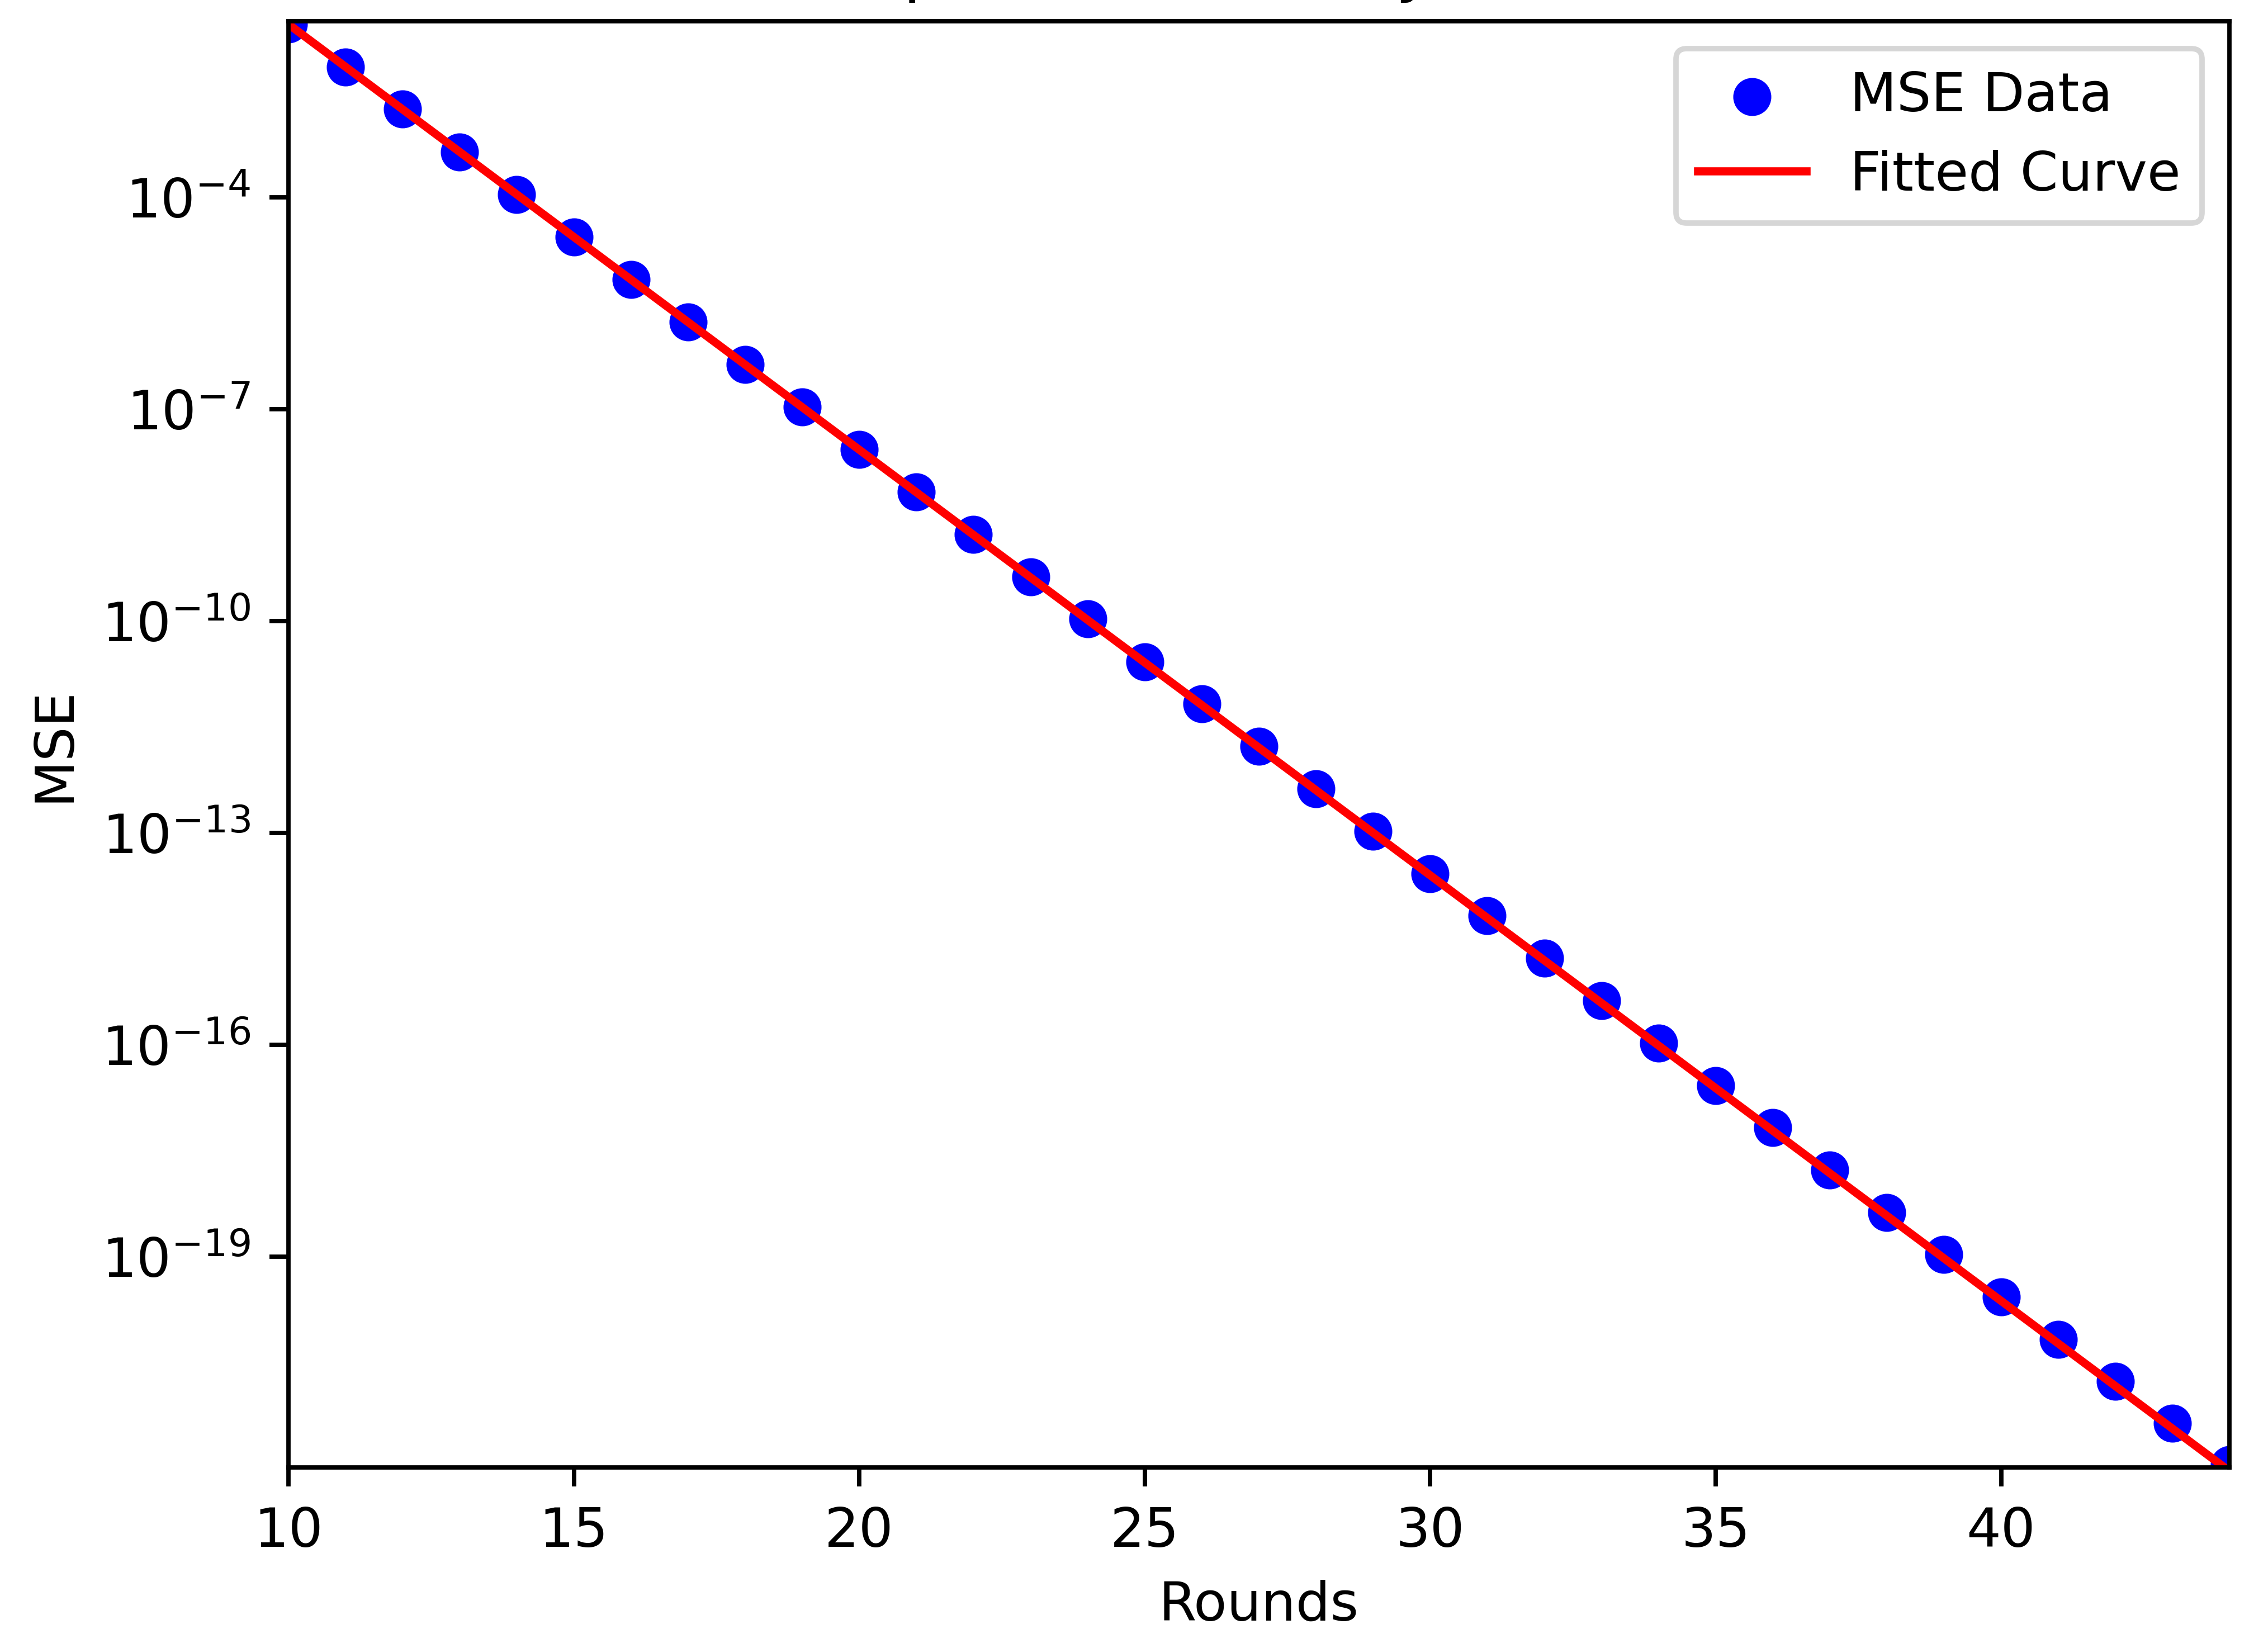
\includegraphics{figures/Simulation_outcomes/StarGraph/PPS/PPS_modelfitting_rounds_44_model_1.png}}
    \caption{Star graph - exponential regression fit: PPS}
    \label{fig:ppsStarModelFit}
\end{figure}
\begin{figure}[]
    \centering
    \scalebox{0.8}{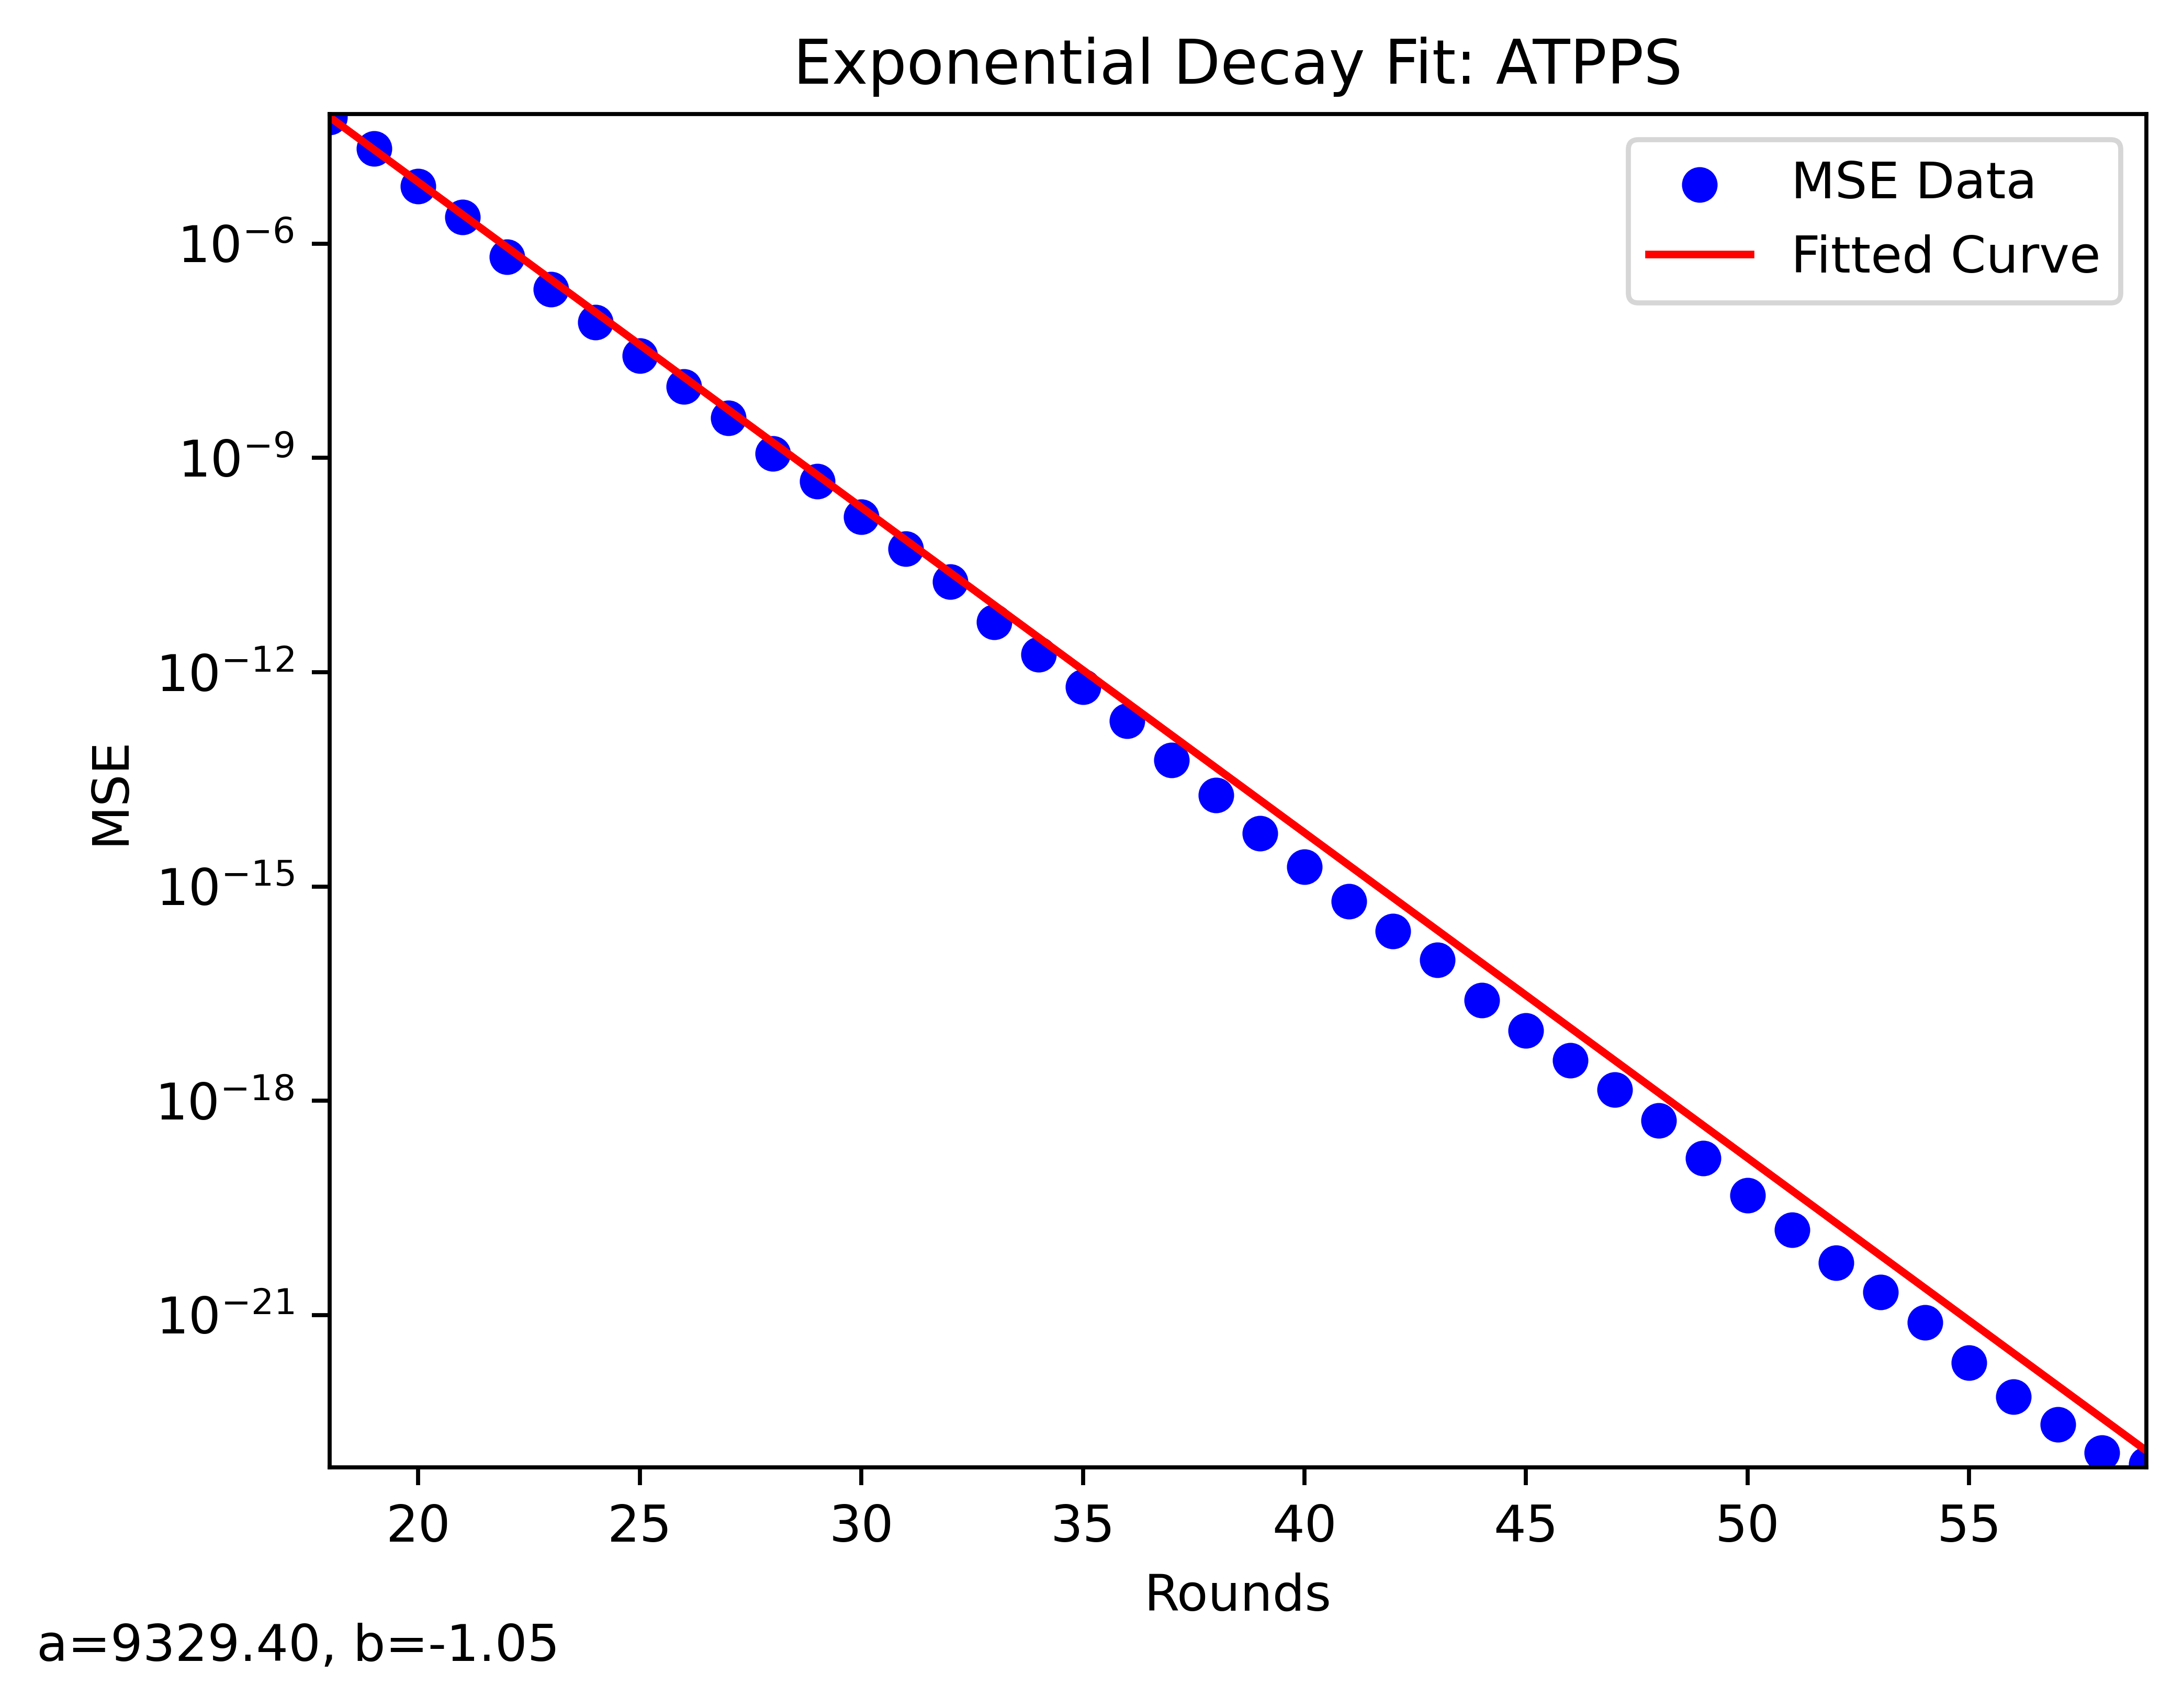
\includegraphics{figures/Simulation_outcomes/StarGraph/ATPPS/ATPPS_modelfitting_rounds_59_model_1.png}}
    \caption{Star graph - exponential regression fit: ATPPS}
    \label{fig:atppsStarModelFit}
\end{figure}
\begin{figure}
    \centering
    \scalebox{0.8}{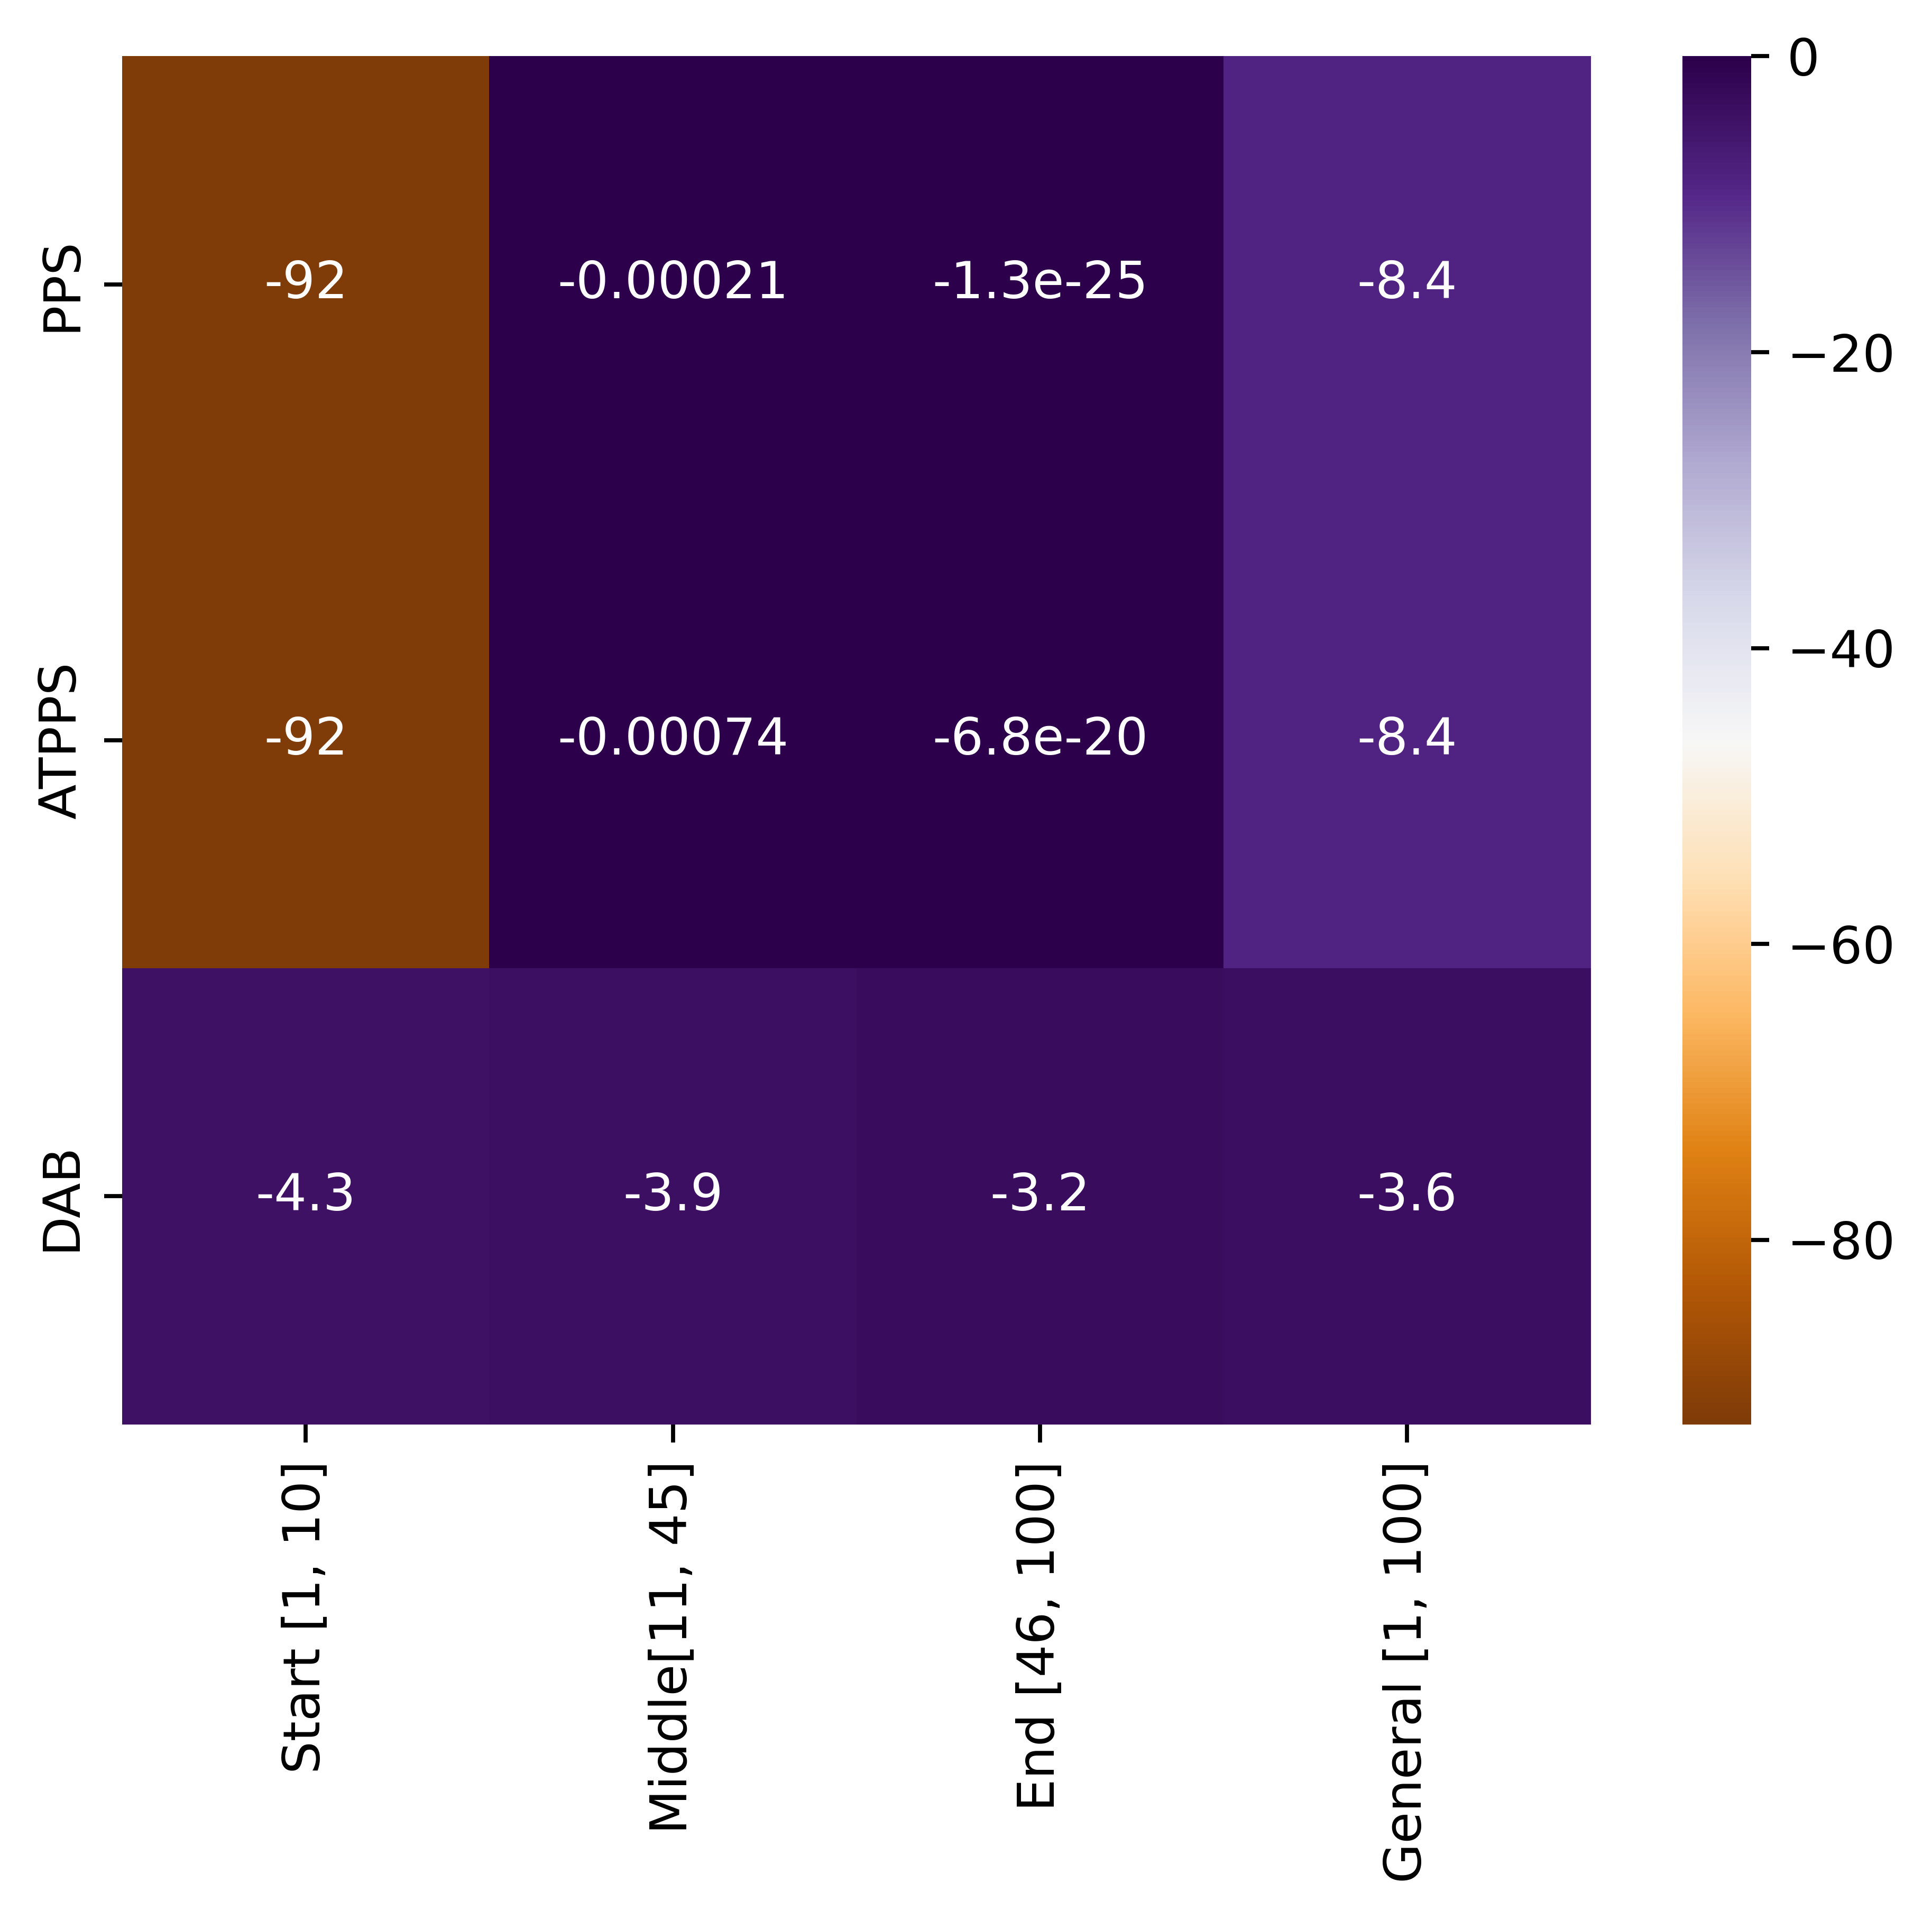
\includegraphics{figures/Simulation_outcomes/StarGraph/DAB_vs_PPS_vs_ATPPS_slopesheatmap_100rounds.png}}
    \caption{Star graph: heat map of slopes per region}
    \label{fig:stargraphslopes}
\end{figure}

\section{Ring Graph}\label{sec:ringgraph}
The DAB curve in figure \ref{fig:ringgraphMSEperRoundLogLog} shows the steepest decline in error in the first few rounds of the simulation. The slope of the first 10 rounds is $-84$ for the DAB curve compared to $-82$ for each Push-Pull Sum based algorithm as depicted in figure \ref{fig:ringgraphslopes}. The near-overlap of PPS and ATPPS across the 100 rounds of simulation suggests that the adaptive mechanism provides limited additional benefit in a Ring graph, where selecting a random neighbor might already target an optimal load transfer partner. In a Ring topology, each node only interacts with its two immediate neighbors. The adaptive threshold mechanism relies on significant load differences between nodes to trigger transfers, but in a Ring graph, local variations might not be substantial enough to make the threshold mechanism advantageous. For the PPS, every node communicates with its neighbors in every round. This constant exchange ensures rapid propagation of load. The adaptive threshold might reduce some of these exchanges; however, in a Ring graph, where the network diameter is large, reducing communication might delay convergence rather than improve it. The threshold mechanism could therefore counteract its own benefits and limit its advantage over the PPS. The DAB function performs better in this scenario since it always interacts with the optimal partner to exchange loads. The benefit of randomness vanishes for a network topology where each node only has two neighbors, and a deterministic approach actually performs better.

The MSE data from each algorithm's simulations were fitted to a polynomial regression model of degree 4. The best-fit model for the DAB MSE data for rounds 10 to 60 follows the equation: $MSE_r=1.72\times 10^{-5}r^{4}-2.30\times 10^{-3}r^{3}+ 0.19r^{2}-5.99r+114.83$ as shown in figure \ref{fig:dabRingModelFit}. A similar polynomial model was fitted for the PPS and ATPPS curves: $MSE_r= 2.99\times 10^{-5}r^{4}-0.5\times 10^{-2}r^{3} + 0.32r^{2} -9.68r + 166.30$ for the PPS curve as shown in figure \ref{fig:ppsRingModelFit}, and $MSE_r=3.04\times 10^{-5}r^{4}-0.5\times 10^{-2}r^{3} + 0.32r^{2}-9.64r+161.86$ for the ATPPS curve as depicted in figure \ref{fig:atppsRingModelFit}.

\begin{figure}[]
    \centering
    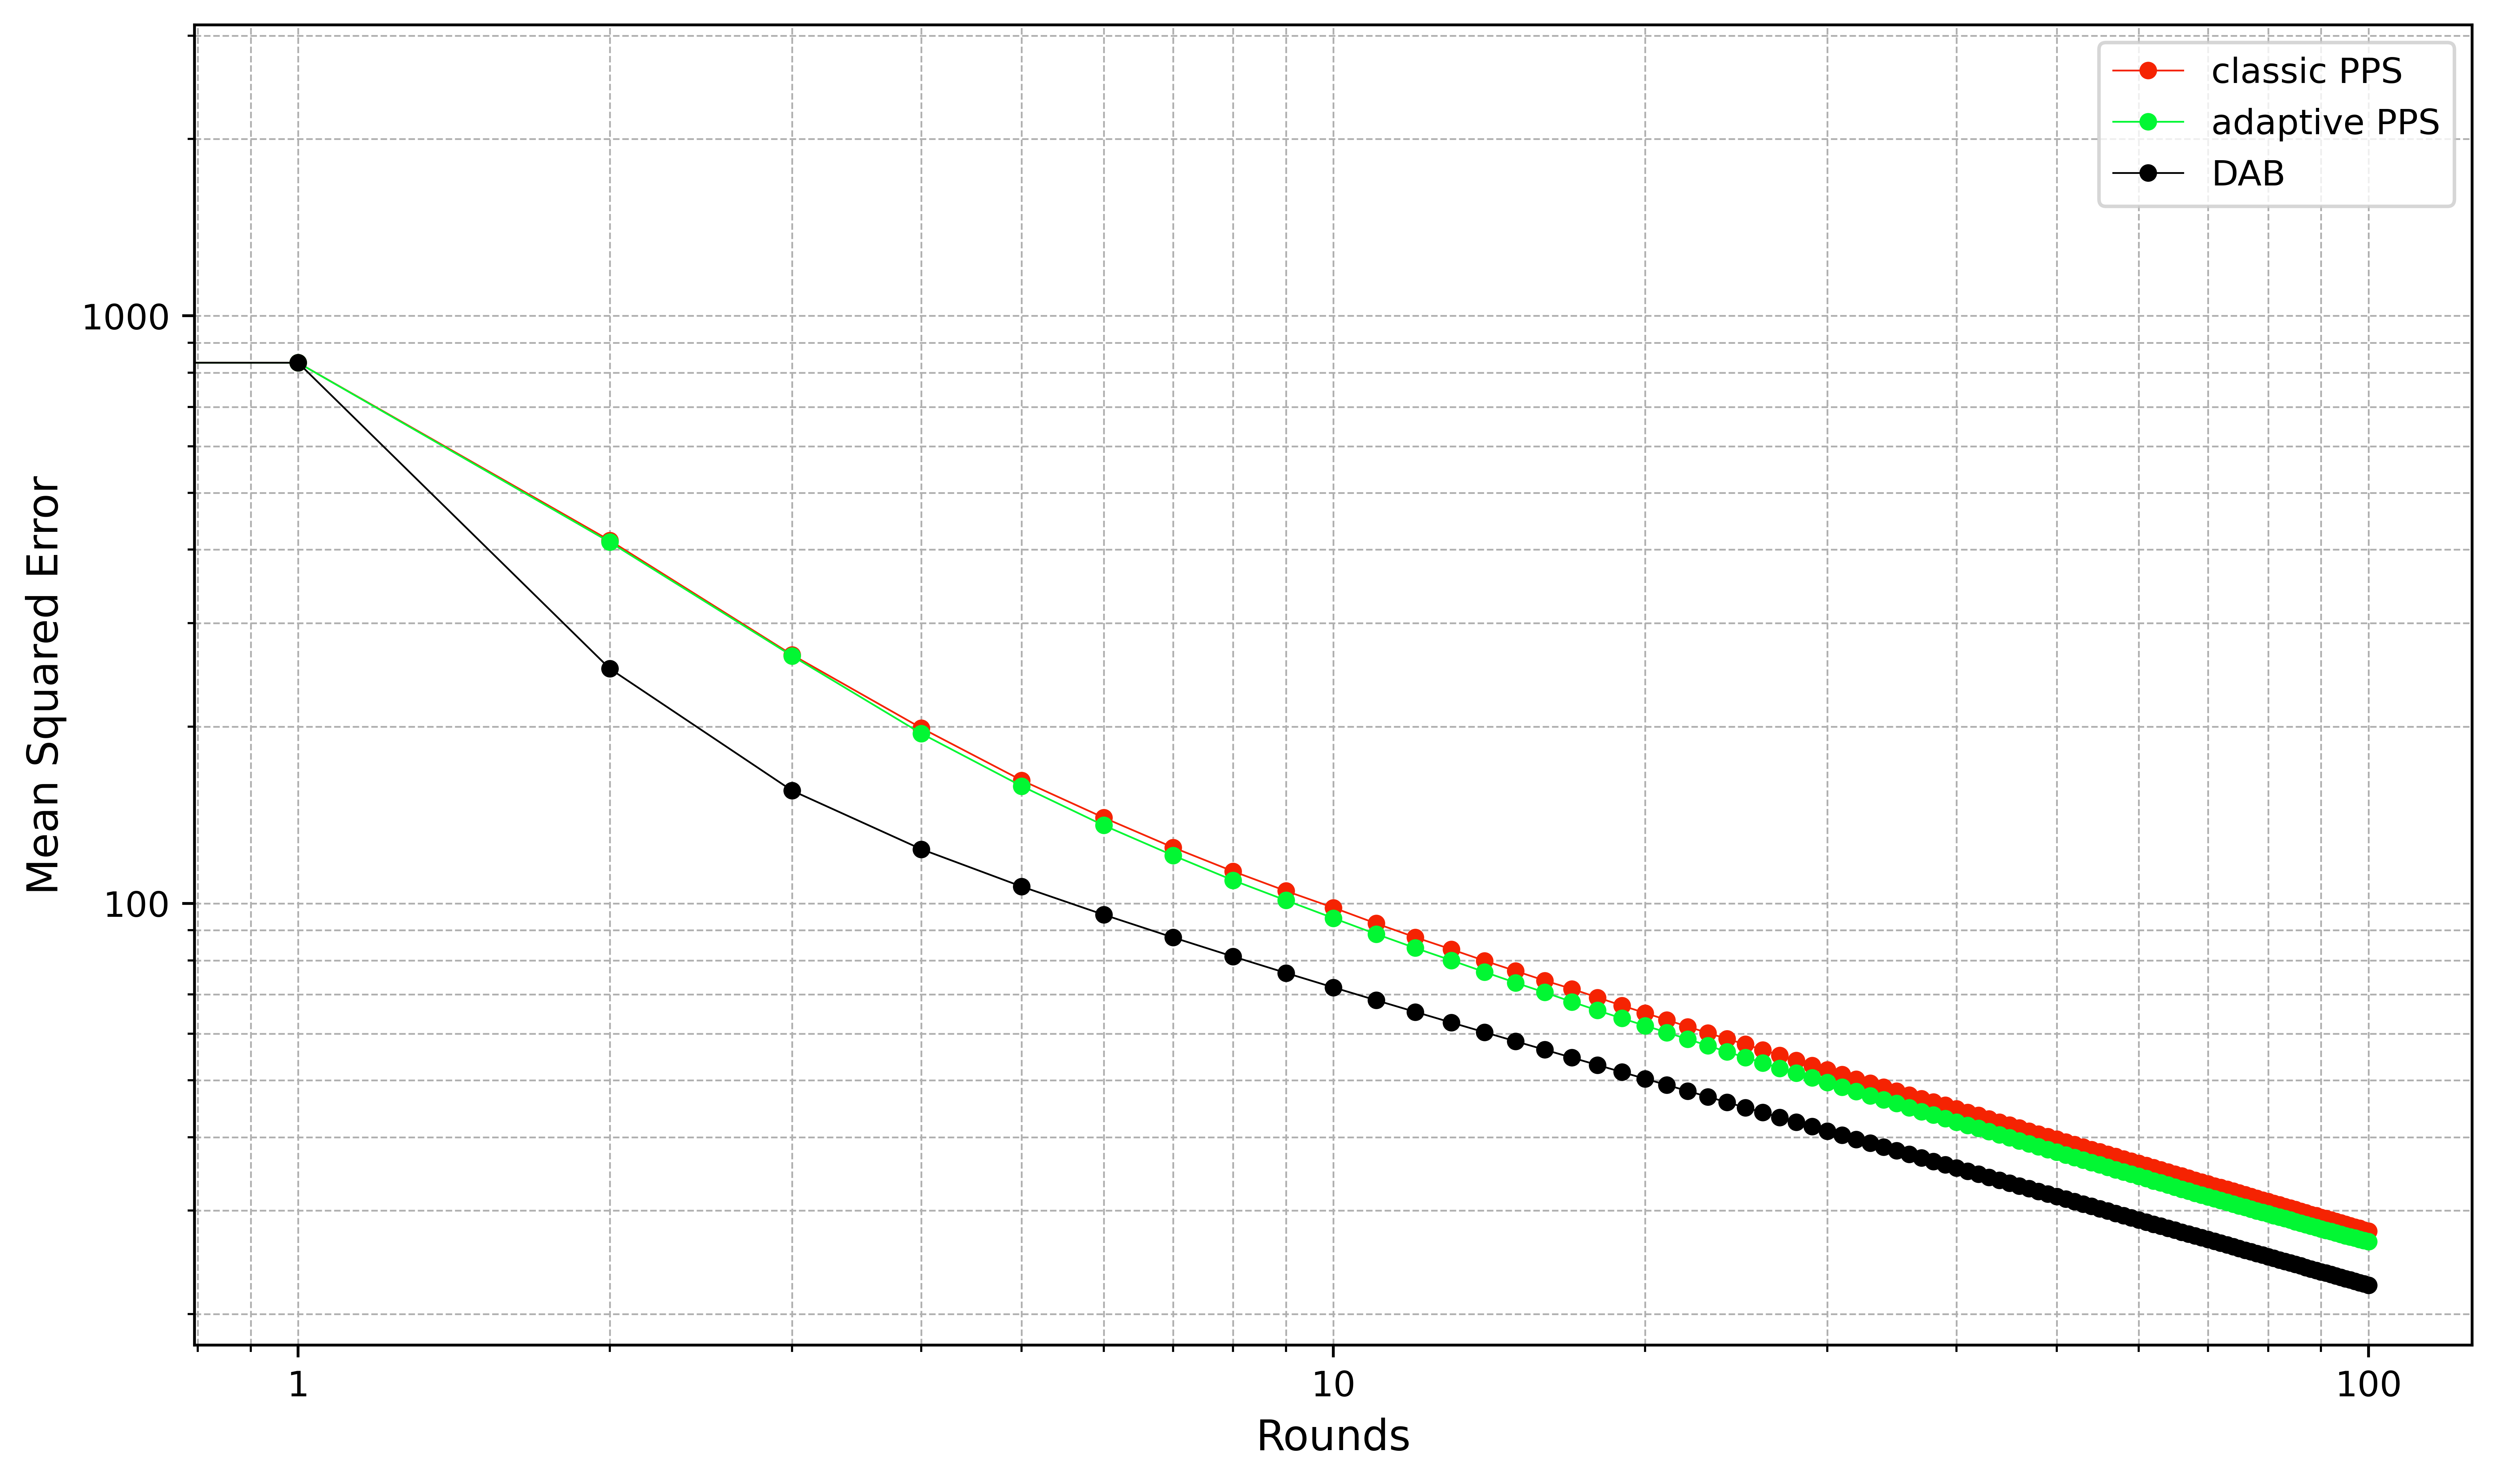
\includegraphics[width=\linewidth]{figures/Simulation_outcomes/RingGraph/DAB_vs_PPS_RG_r100_n1024_averaged_loglog.png}
    \caption{Ring graph: mean squared error per rounds (log-log)}
    \label{fig:ringgraphMSEperRoundLogLog}
\end{figure}
\begin{figure}[]
    \centering
    \scalebox{0.8}{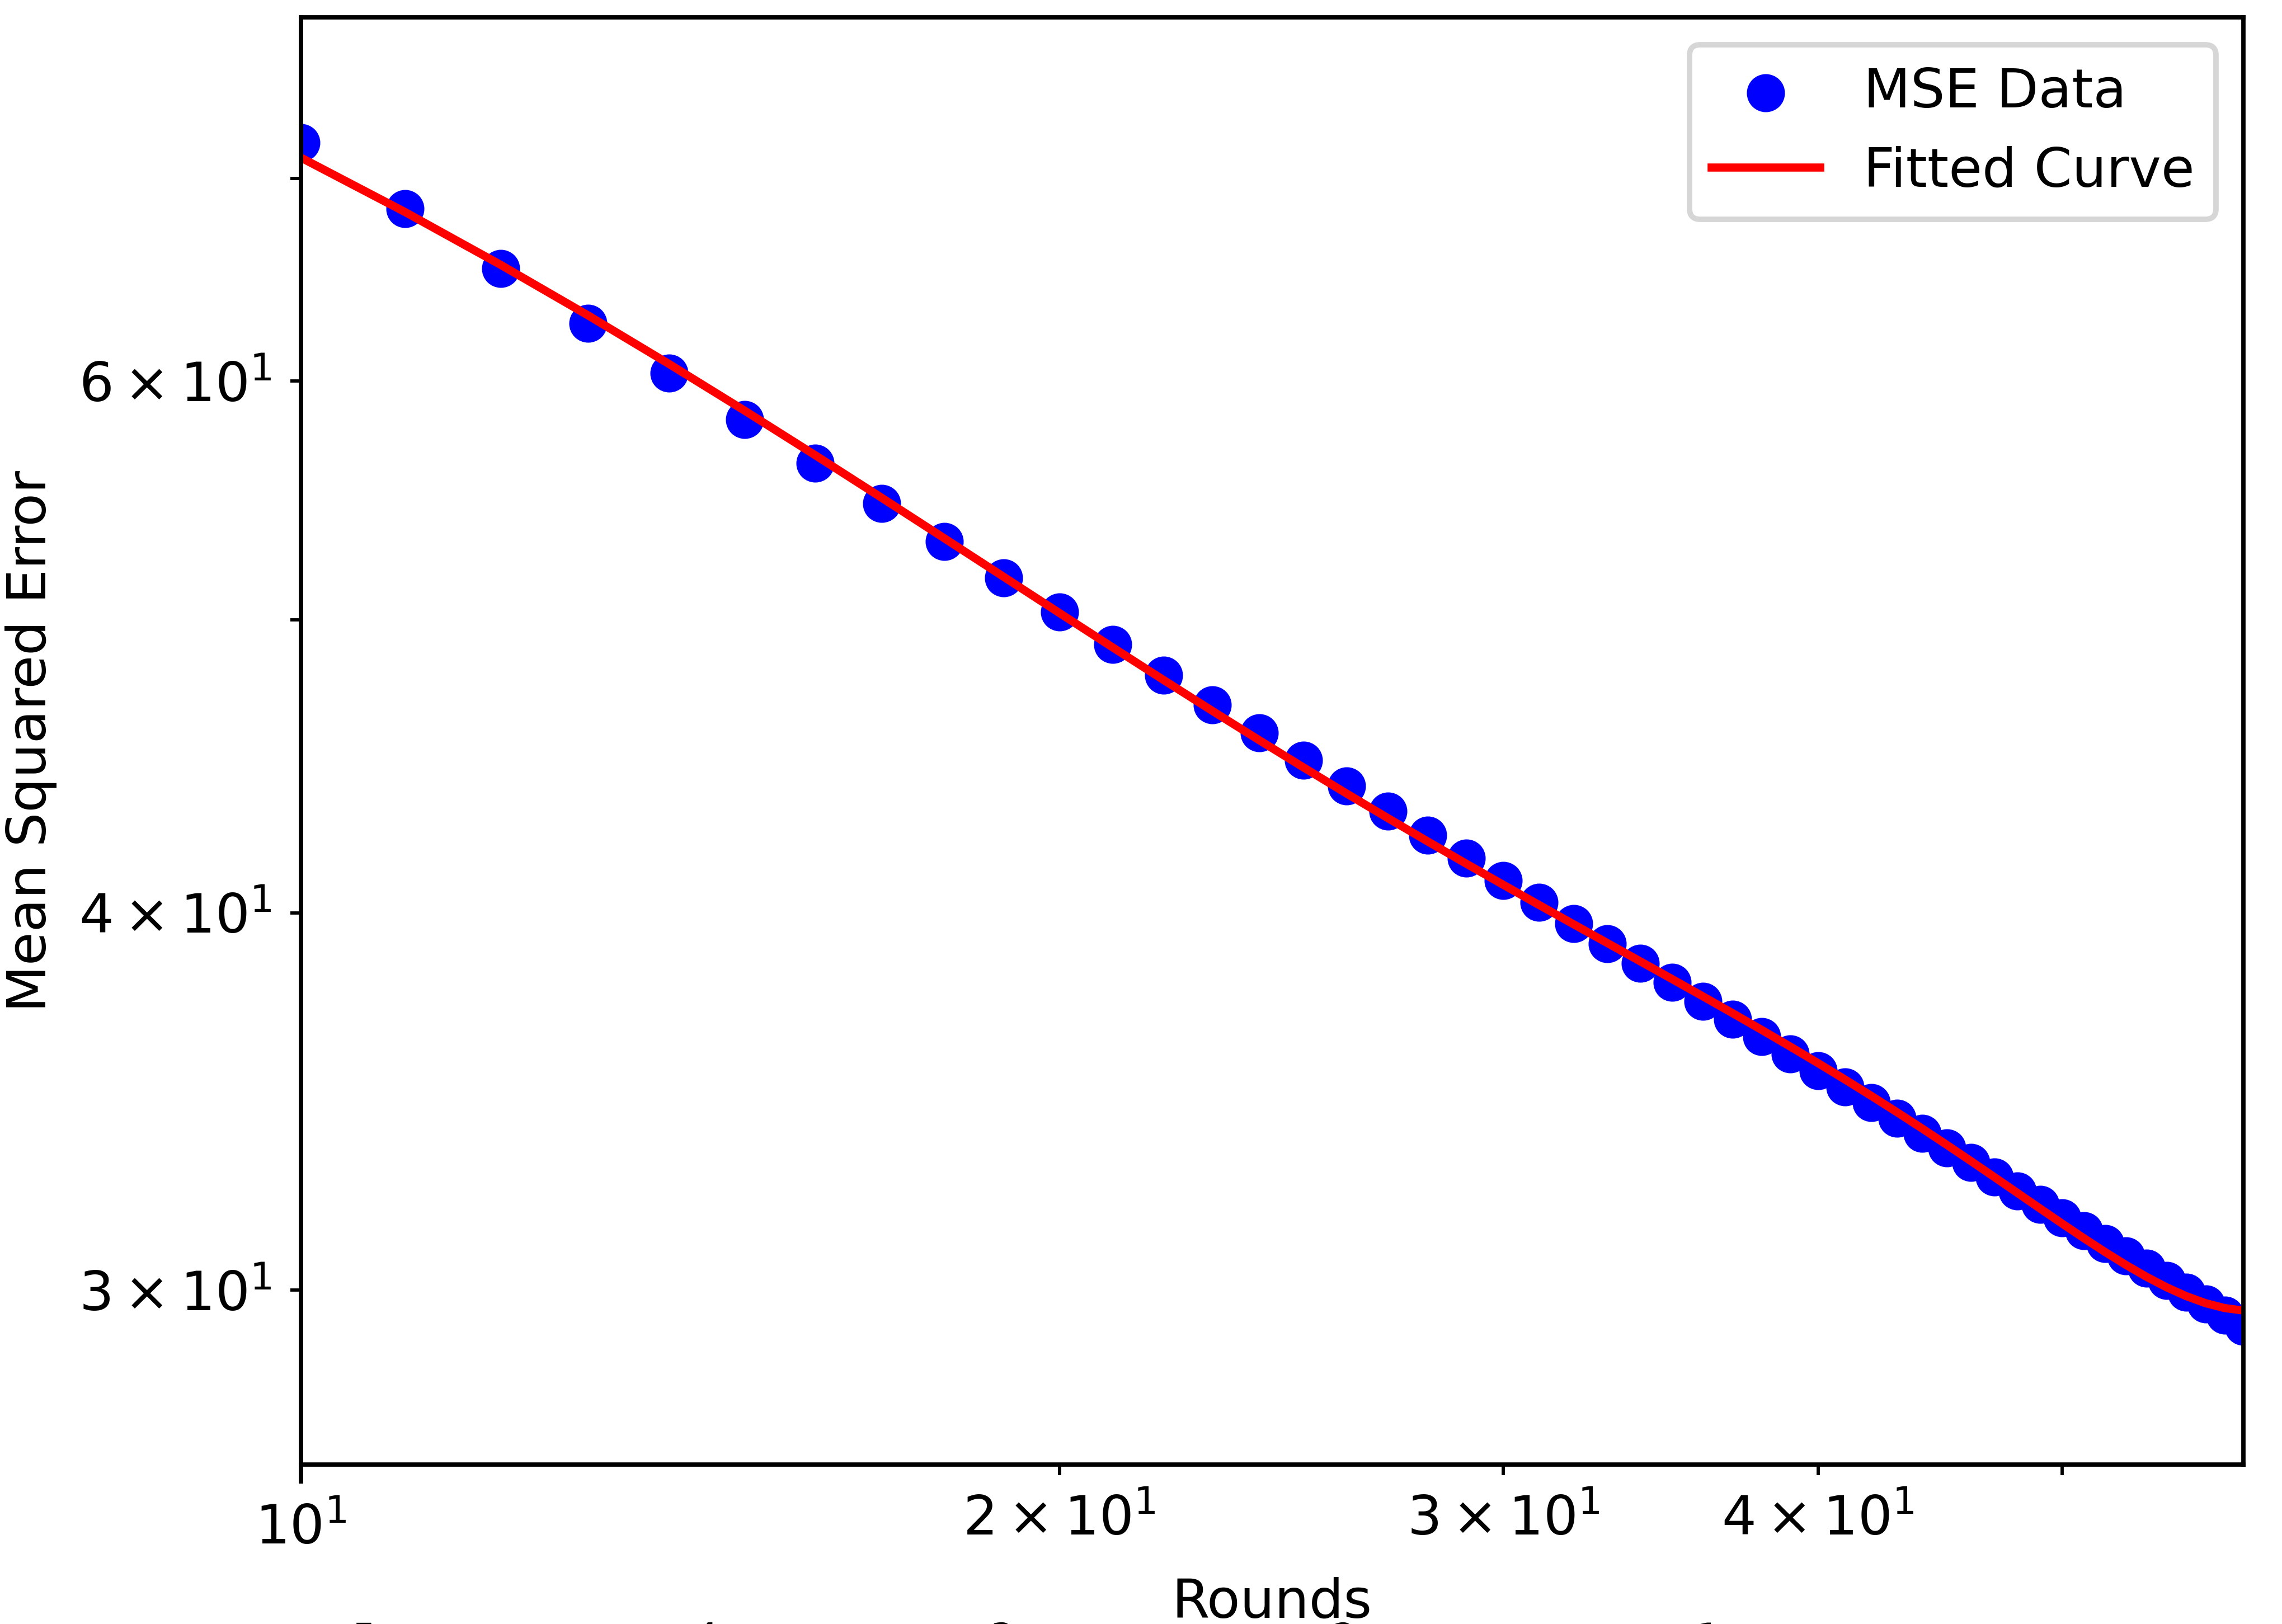
\includegraphics{figures/Simulation_outcomes/RingGraph/DAB/DAB_modelfitting_rounds_59_model_2.png}}
    \caption{Ring graph - polynomial regression fit: DAB}
    \label{fig:dabRingModelFit}
\end{figure}
\begin{figure}[]
   \centering
   \scalebox{0.8}{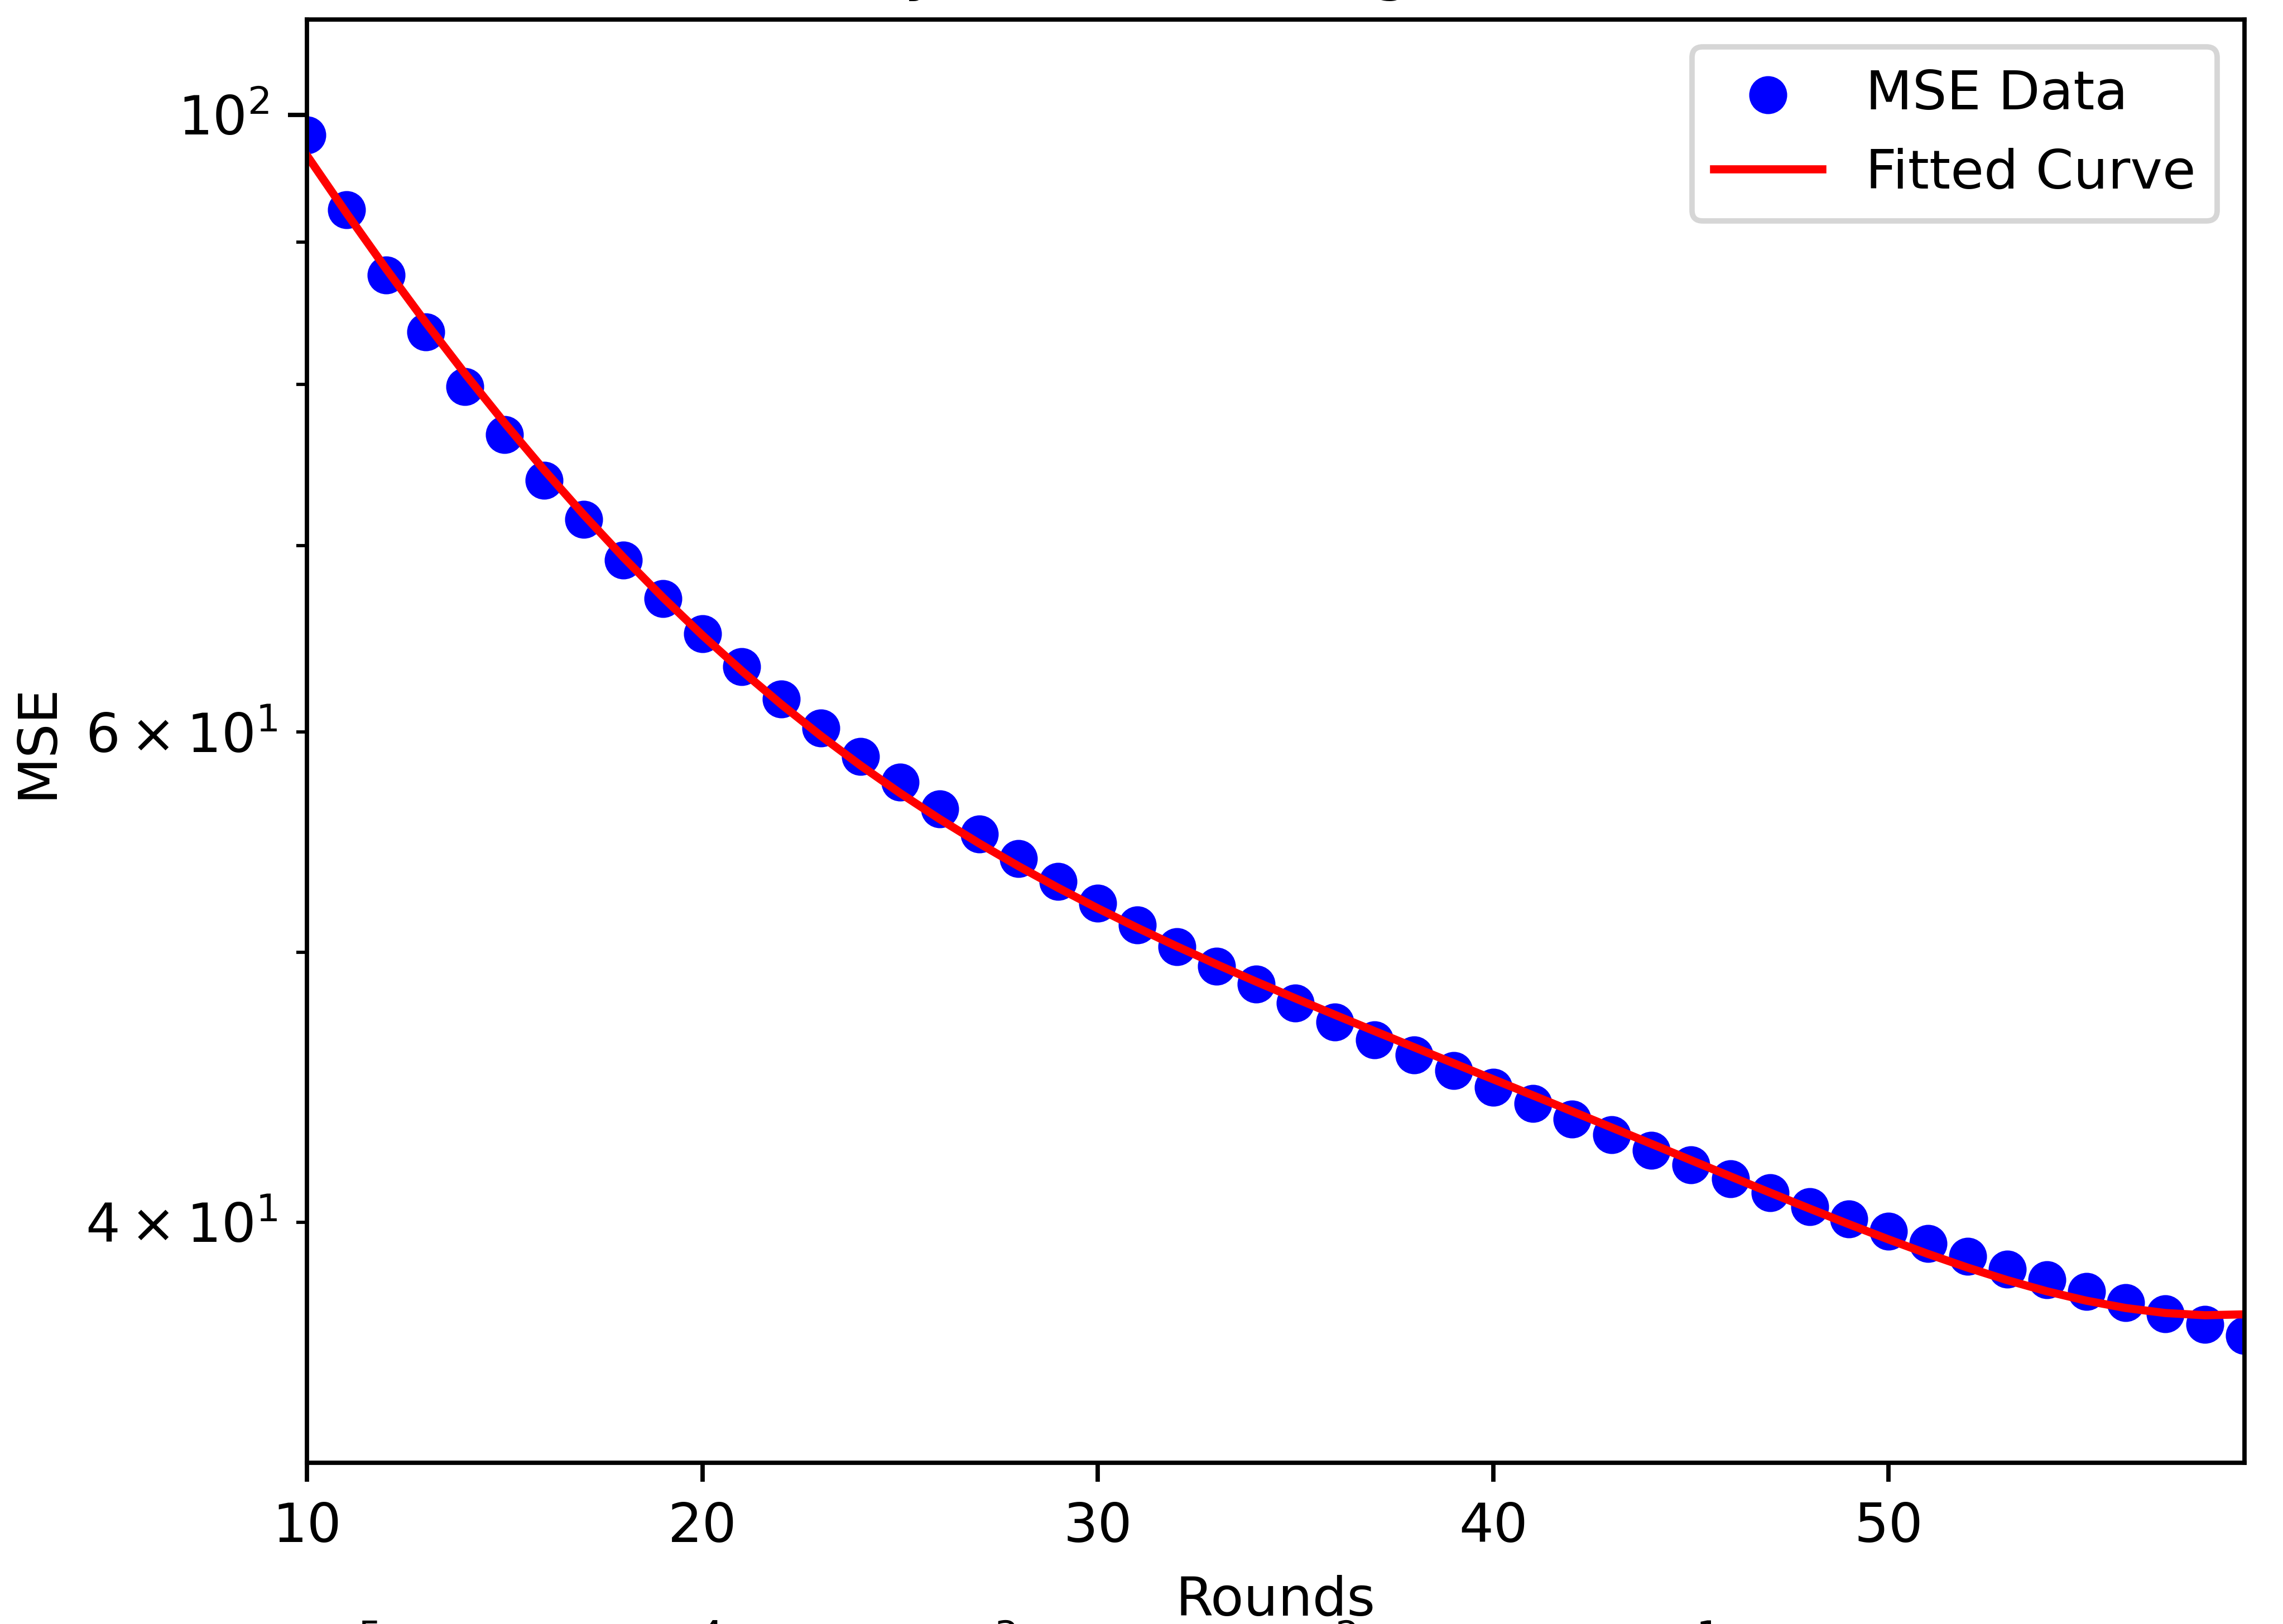
\includegraphics{figures/Simulation_outcomes/RingGraph/PPS/PPS_modelfitting_rounds_59_model_2.png}}
   \caption{Ring graph - polynomial regression fit: PPS}
   \label{fig:ppsRingModelFit}
\end{figure}
\begin{figure}[]
    \centering
    \scalebox{0.8}{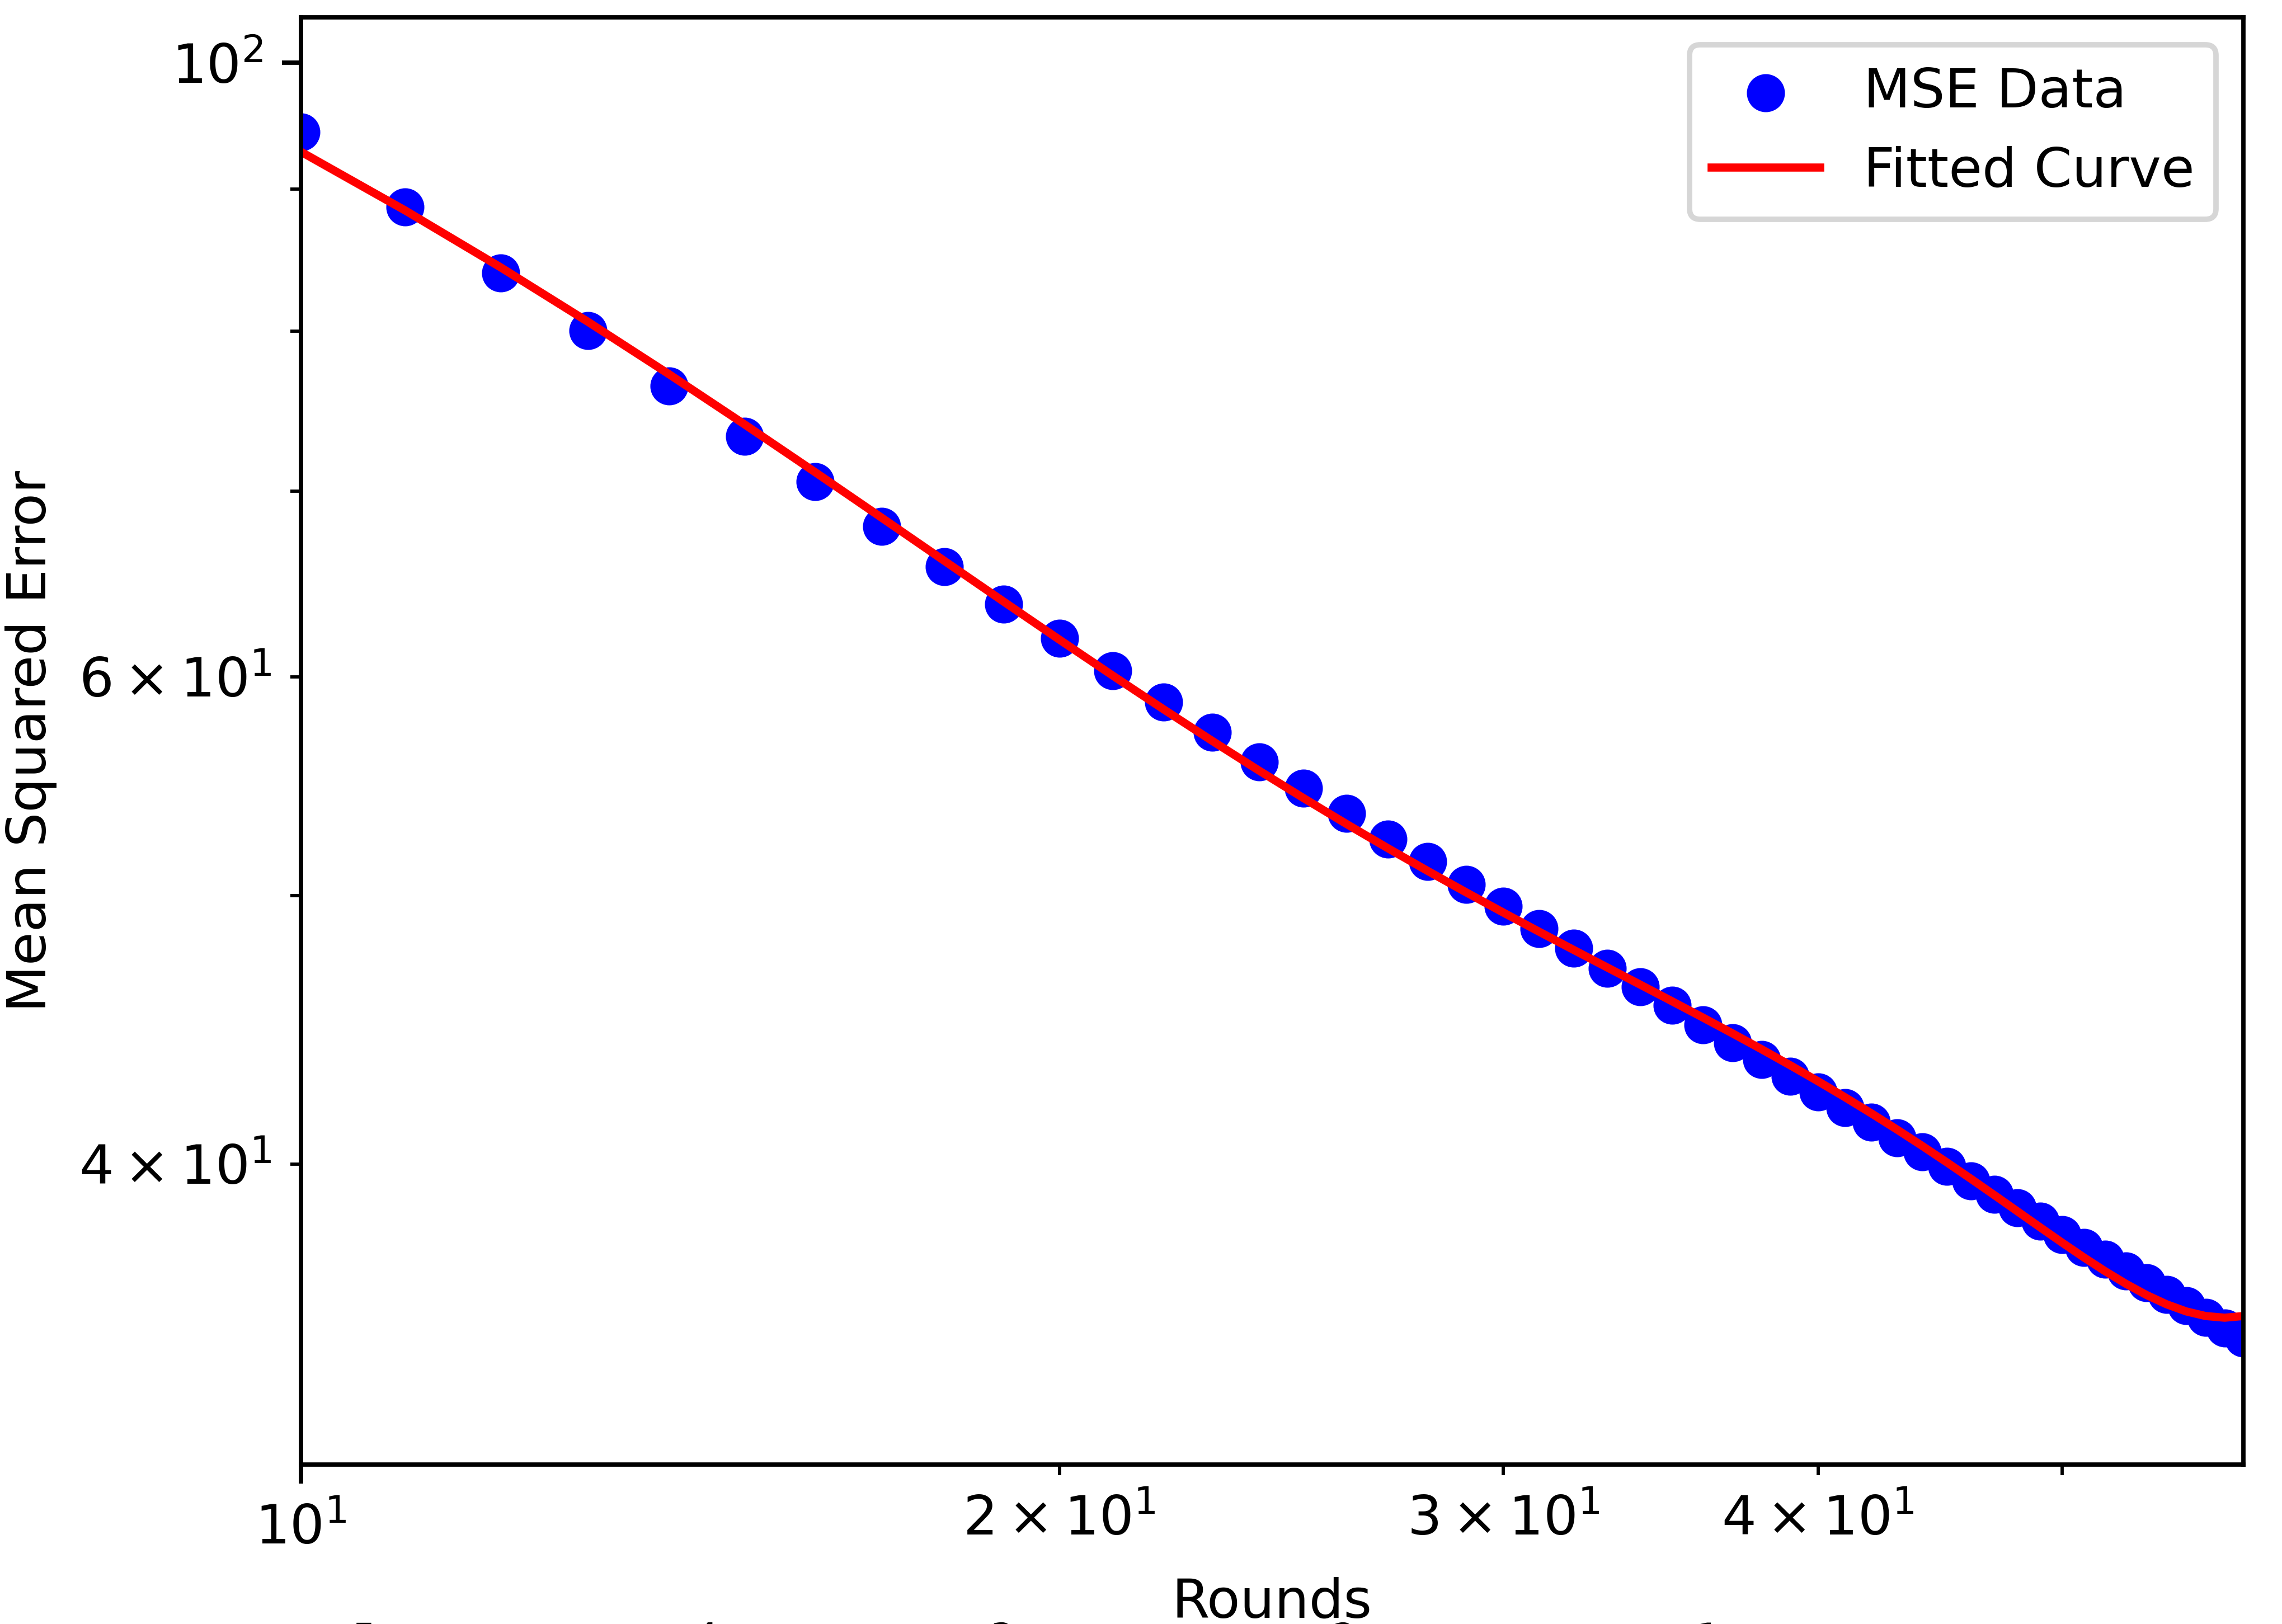
\includegraphics{figures/Simulation_outcomes/RingGraph/ATPPS/ATPPS_modelfitting_rounds_59_model_2.png}}
    \caption{Ring graph - polynomial regression fit: ATPPS}
    \label{fig:atppsRingModelFit}
\end{figure}
\begin{figure}
    \centering
    \scalebox{0.8}{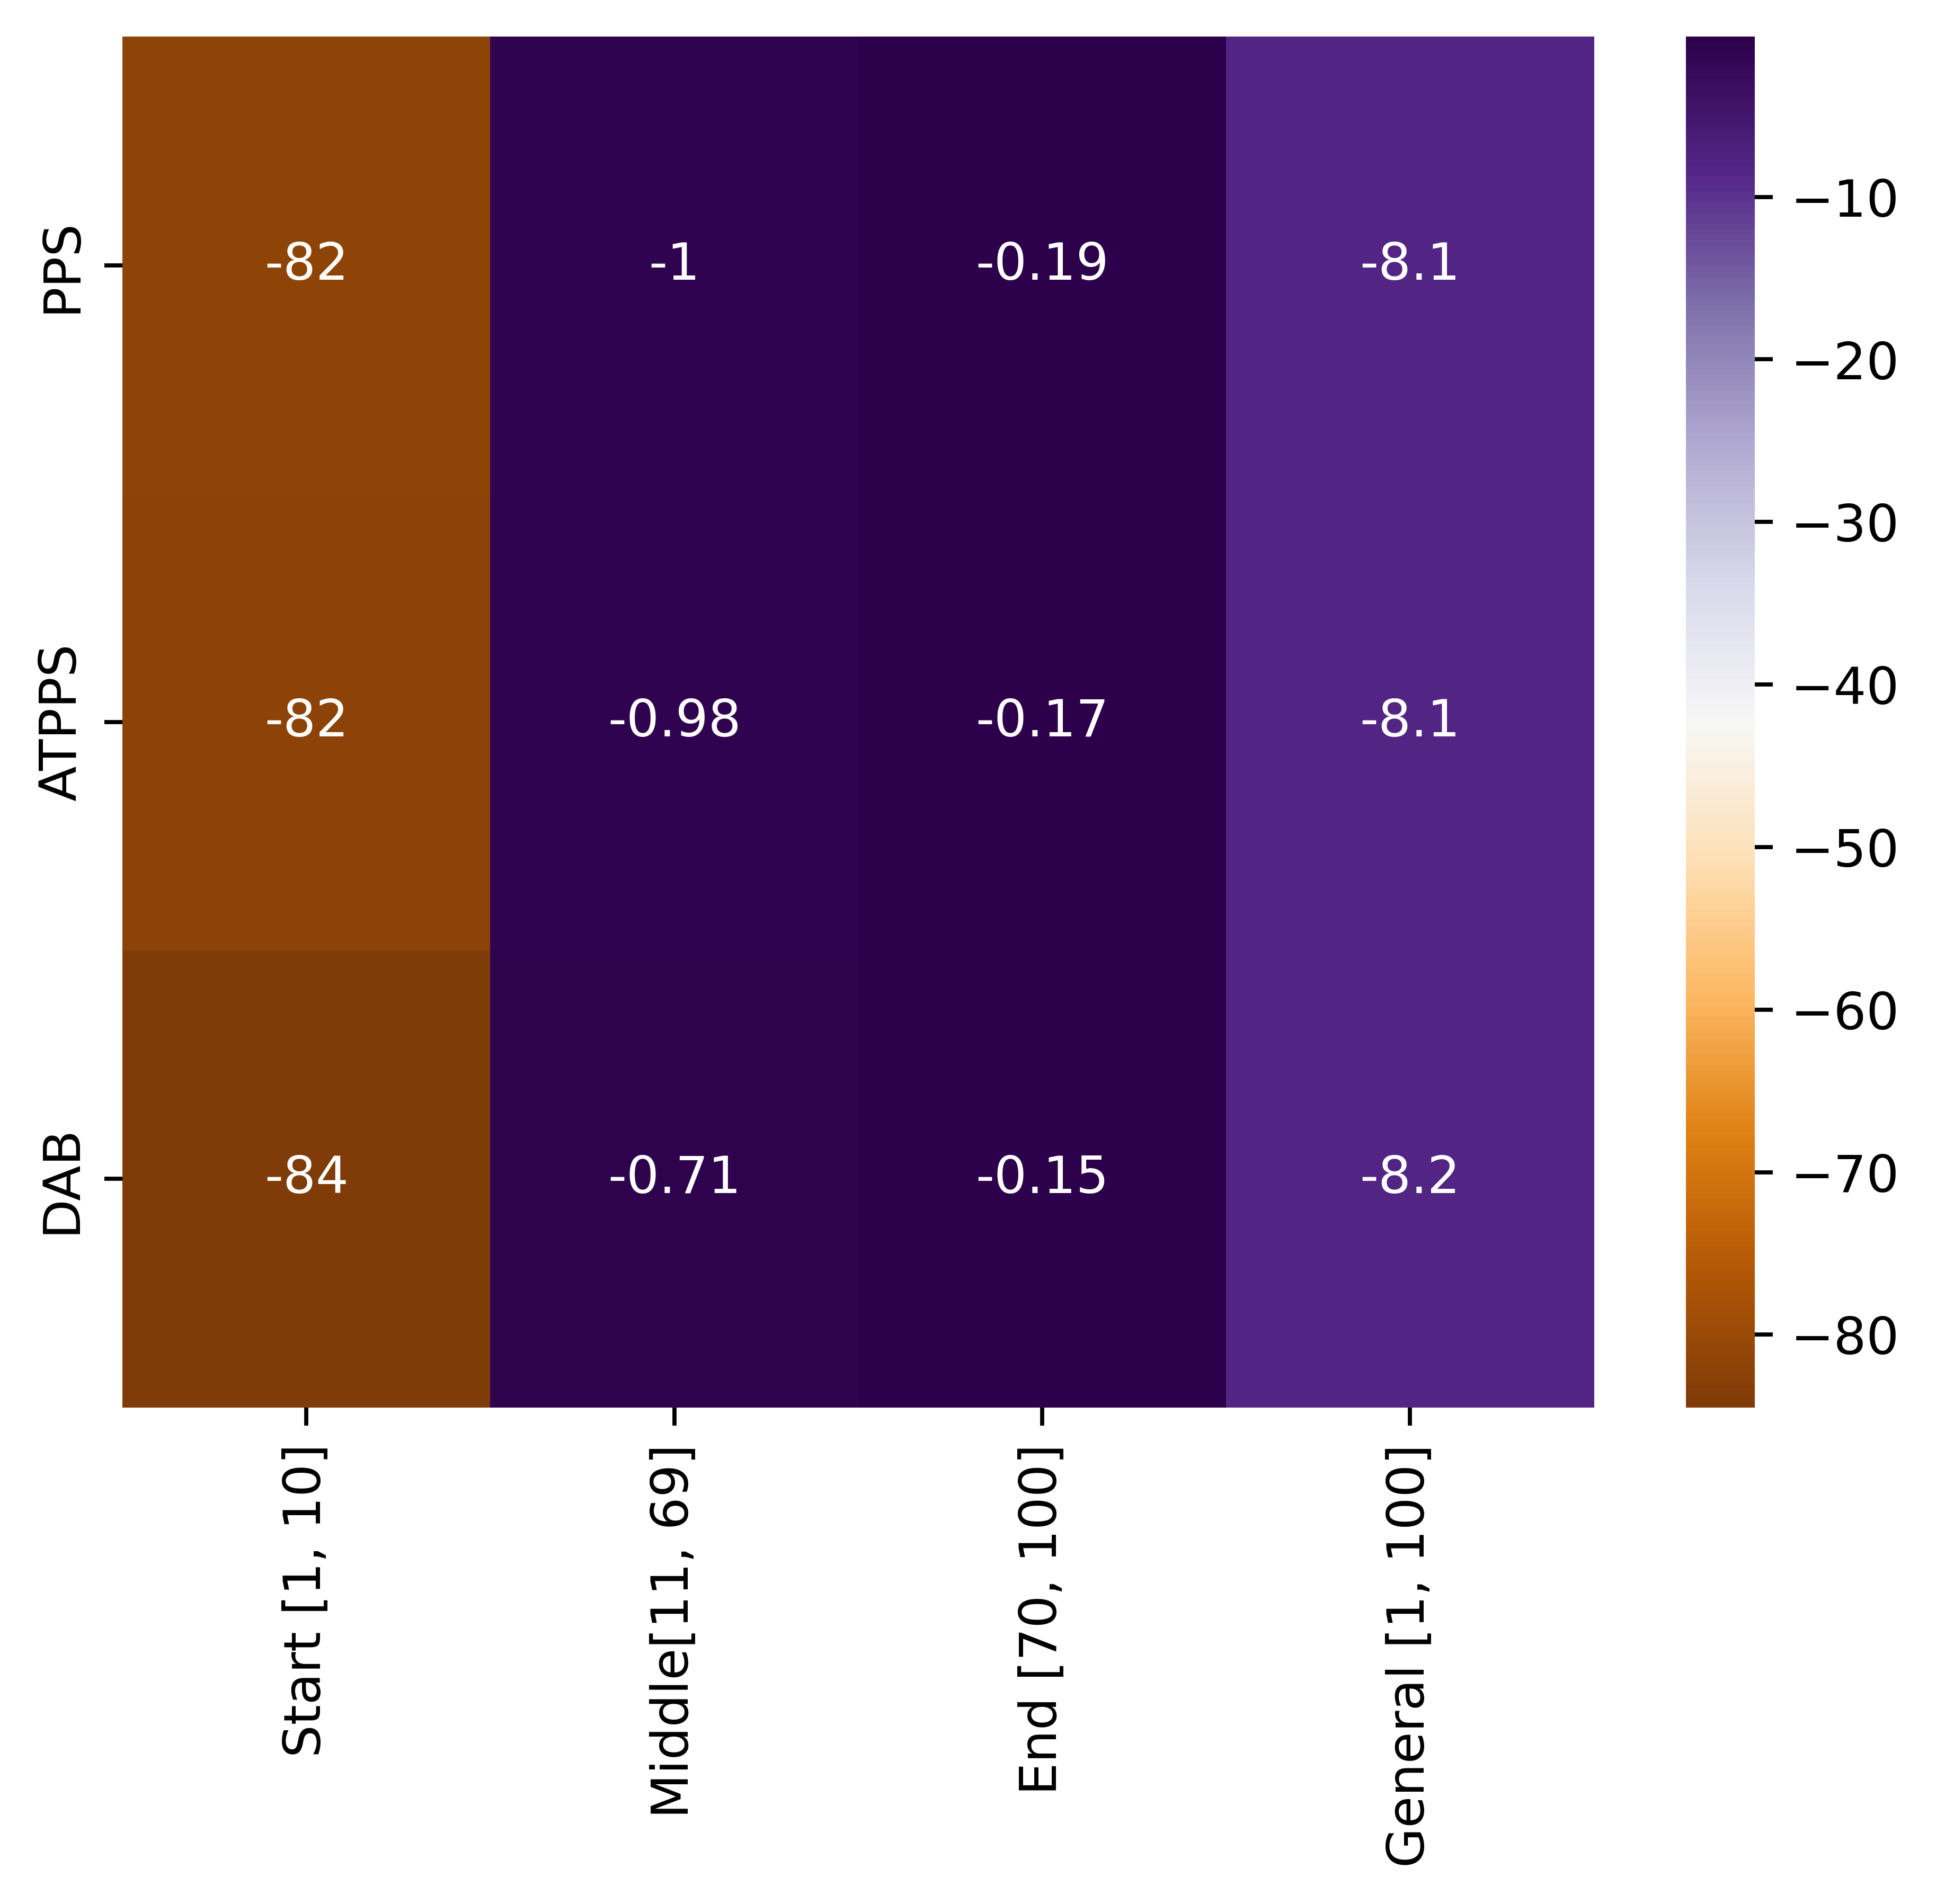
\includegraphics{figures/Simulation_outcomes/RingGraph/DAB_vs_PPS_vs_ATPPS_slopesheatmap_100rounds.png}}
    \caption{Ring graph: heat map of slopes per region}
    \label{fig:ringgraphslopes}
\end{figure}

\section{Torus Grid Graph}\label{sec:torusgridGraph}
Figure \ref{fig:torusMSEperRoundLogLog} shows the MSE reduction over rounds on a Torus Grid graph, plotted on a log-log scale. The DAB curve appears to have a slightly faster initial reduction compared to PPS' and ATPPS' curves in the beginning (rounds 1 to 7). The slope in this region is superior for the DAB algorithm with a value of -140 compared to -130 for the Push-Pull Sum based algorithms (figure \ref{fig:torusgraphslopes}). The PPS and ATPPS curves maintain nearly identical performances during the middle region (rounds 8 to 40), reducing MSE at a similar rate, with a slope of -1 for the PPS curve and -0.83 for the ATPPS curve. DAB shows a noticeable improvement in reducing the imbalance compared to both PPS and ATPPS, achieving lower MSE values consistently. This suggests that DAB adapts more efficiently to the graph's structure during intermediate rounds. In the final region (rounds 41 to 100), DAB continues to reduce MSE more effectively than the Push-Pull Sum-based protocols. PPS and ATPPS exhibit convergence, but they lag behind the DAB algorithm in reaching minimal MSE. Tori have more structured connectivity compared to a Star or Ring graph, allowing better distribution of loads via localized interactions. DAB's deterministic approach benefits from leveraging this regularity, leading to its superior performance. The ATPPS algorithm achieves a balanced trade-off in this scenario. It outperforms the PPS approach, particularly in later rounds, where its adaptive mechanism prevents redundant load transfers and prioritizes exchanges that have a more significant impact on error reduction.

The uniform neighborhood structure of Tori ensures that DAB's deterministic decisions (e.g., always choosing the minimal neighbor) are consistently effective across the graph. The algorithm does not suffer from random suboptimal decisions introduced by probabilistic neighbor choices, making it well-suited to the topology. Both PPS and ATPPS protocols rely on randomly selecting a neighbor for load exchange. While this randomness is beneficial in irregular or dense graphs (e.g., Star or Complete graphs), it is less effective in structured topologies compared to the DAB, like a Torus Grid. The Push-Pull Sum based algorithms do not always target the most unbalanced areas. This means that load propagation can sometimes "stall" in certain regions, requiring more rounds to achieve global balance. The ATTPS draws its benefit over the PPS (especially in later rounds) by deciding which option of the available subset is the best. The discrepancy between the two load balancing algorithms widens in the last few rounds as trades between two nodes with higher load differences are more impactful once the network is already heavily balanced.

The fitted polynomial curve of degree 5 matches the MSE data for DAB effectively, capturing the non-linear dynamics during rounds 10 to 39 following the equation: $MSE_r=-1.35\times 10^{-6}r^{5}+ 1.89\times 10^{-4}r^{4}-0.01r^{3}+0.30r^{2}-4.6r+34.10$ as shown in figure \ref{fig:dabTorusModelFit} a). This suggests that in the early rounds (rounds 10 to 39), the MSE reduction follows a complex pattern, as the loads propagate to different regions of the graph thanks to the wrap-around edges of the Tori. The higher degree captures these dynamics with more precision than simpler models. In later rounds, the performance of the DAB can be captured by a polynomial curve of degree 3 with the equation: $MSE_r=-6.01\times 10^{-06}r^{3}+1.66\times 10^{-3}r^{2}-0.16r+6$ (figure \ref{fig:dabTorusModelFit} b)). At this stage, load balancing stabilizes, and the reduction in MSE becomes more linear or gradual. Thus, a lower-degree polynomial suffices to model the behavior in these later rounds. The curve behavior for the PPS and ATPPS are similar to that of the DAB curve expressed for rounds 10 to 39 by the equations: $MSE_r=-5.54\times 10^{-6}r^{5}+7.65\times 10^{-4}r^{4}-0.04r^{3}+1.16r^{2}-16.81r+112.86$ for the PPS (figure \ref{fig:ppsTorusModelFit} a)) and: $MSE_r = -3.65 \times 10^{-6}r^{5} + 5.16 \times 10^{-4}r^{4} - 0.03r^{3} + 0.83r^{2} - 12.52r + 88.16$ for the ATPPS (figure \ref{fig:atppstorusModelFit} a)). The equations that describe the behavior of the two Push-Pull Sum based algorithms are fitted for rounds 40 to 100 for the PPS: $MSE_r = -1.15 \times 10^{-5}r^{3} + 3.205\times 10^{-3}r^{2} - 0.33r + 13.72$ (figure \ref{fig:ppsTorusModelFit} b)) and for the ATPPS is $MSE_r = -9.99 \times 10^{-6}r^{3} + 2.8034\times 10^{-3}r^{2} - 0.28r + 11.29$ (figure \ref{fig:atppstorusModelFit} b)).

\begin{figure}[]
    \centering
    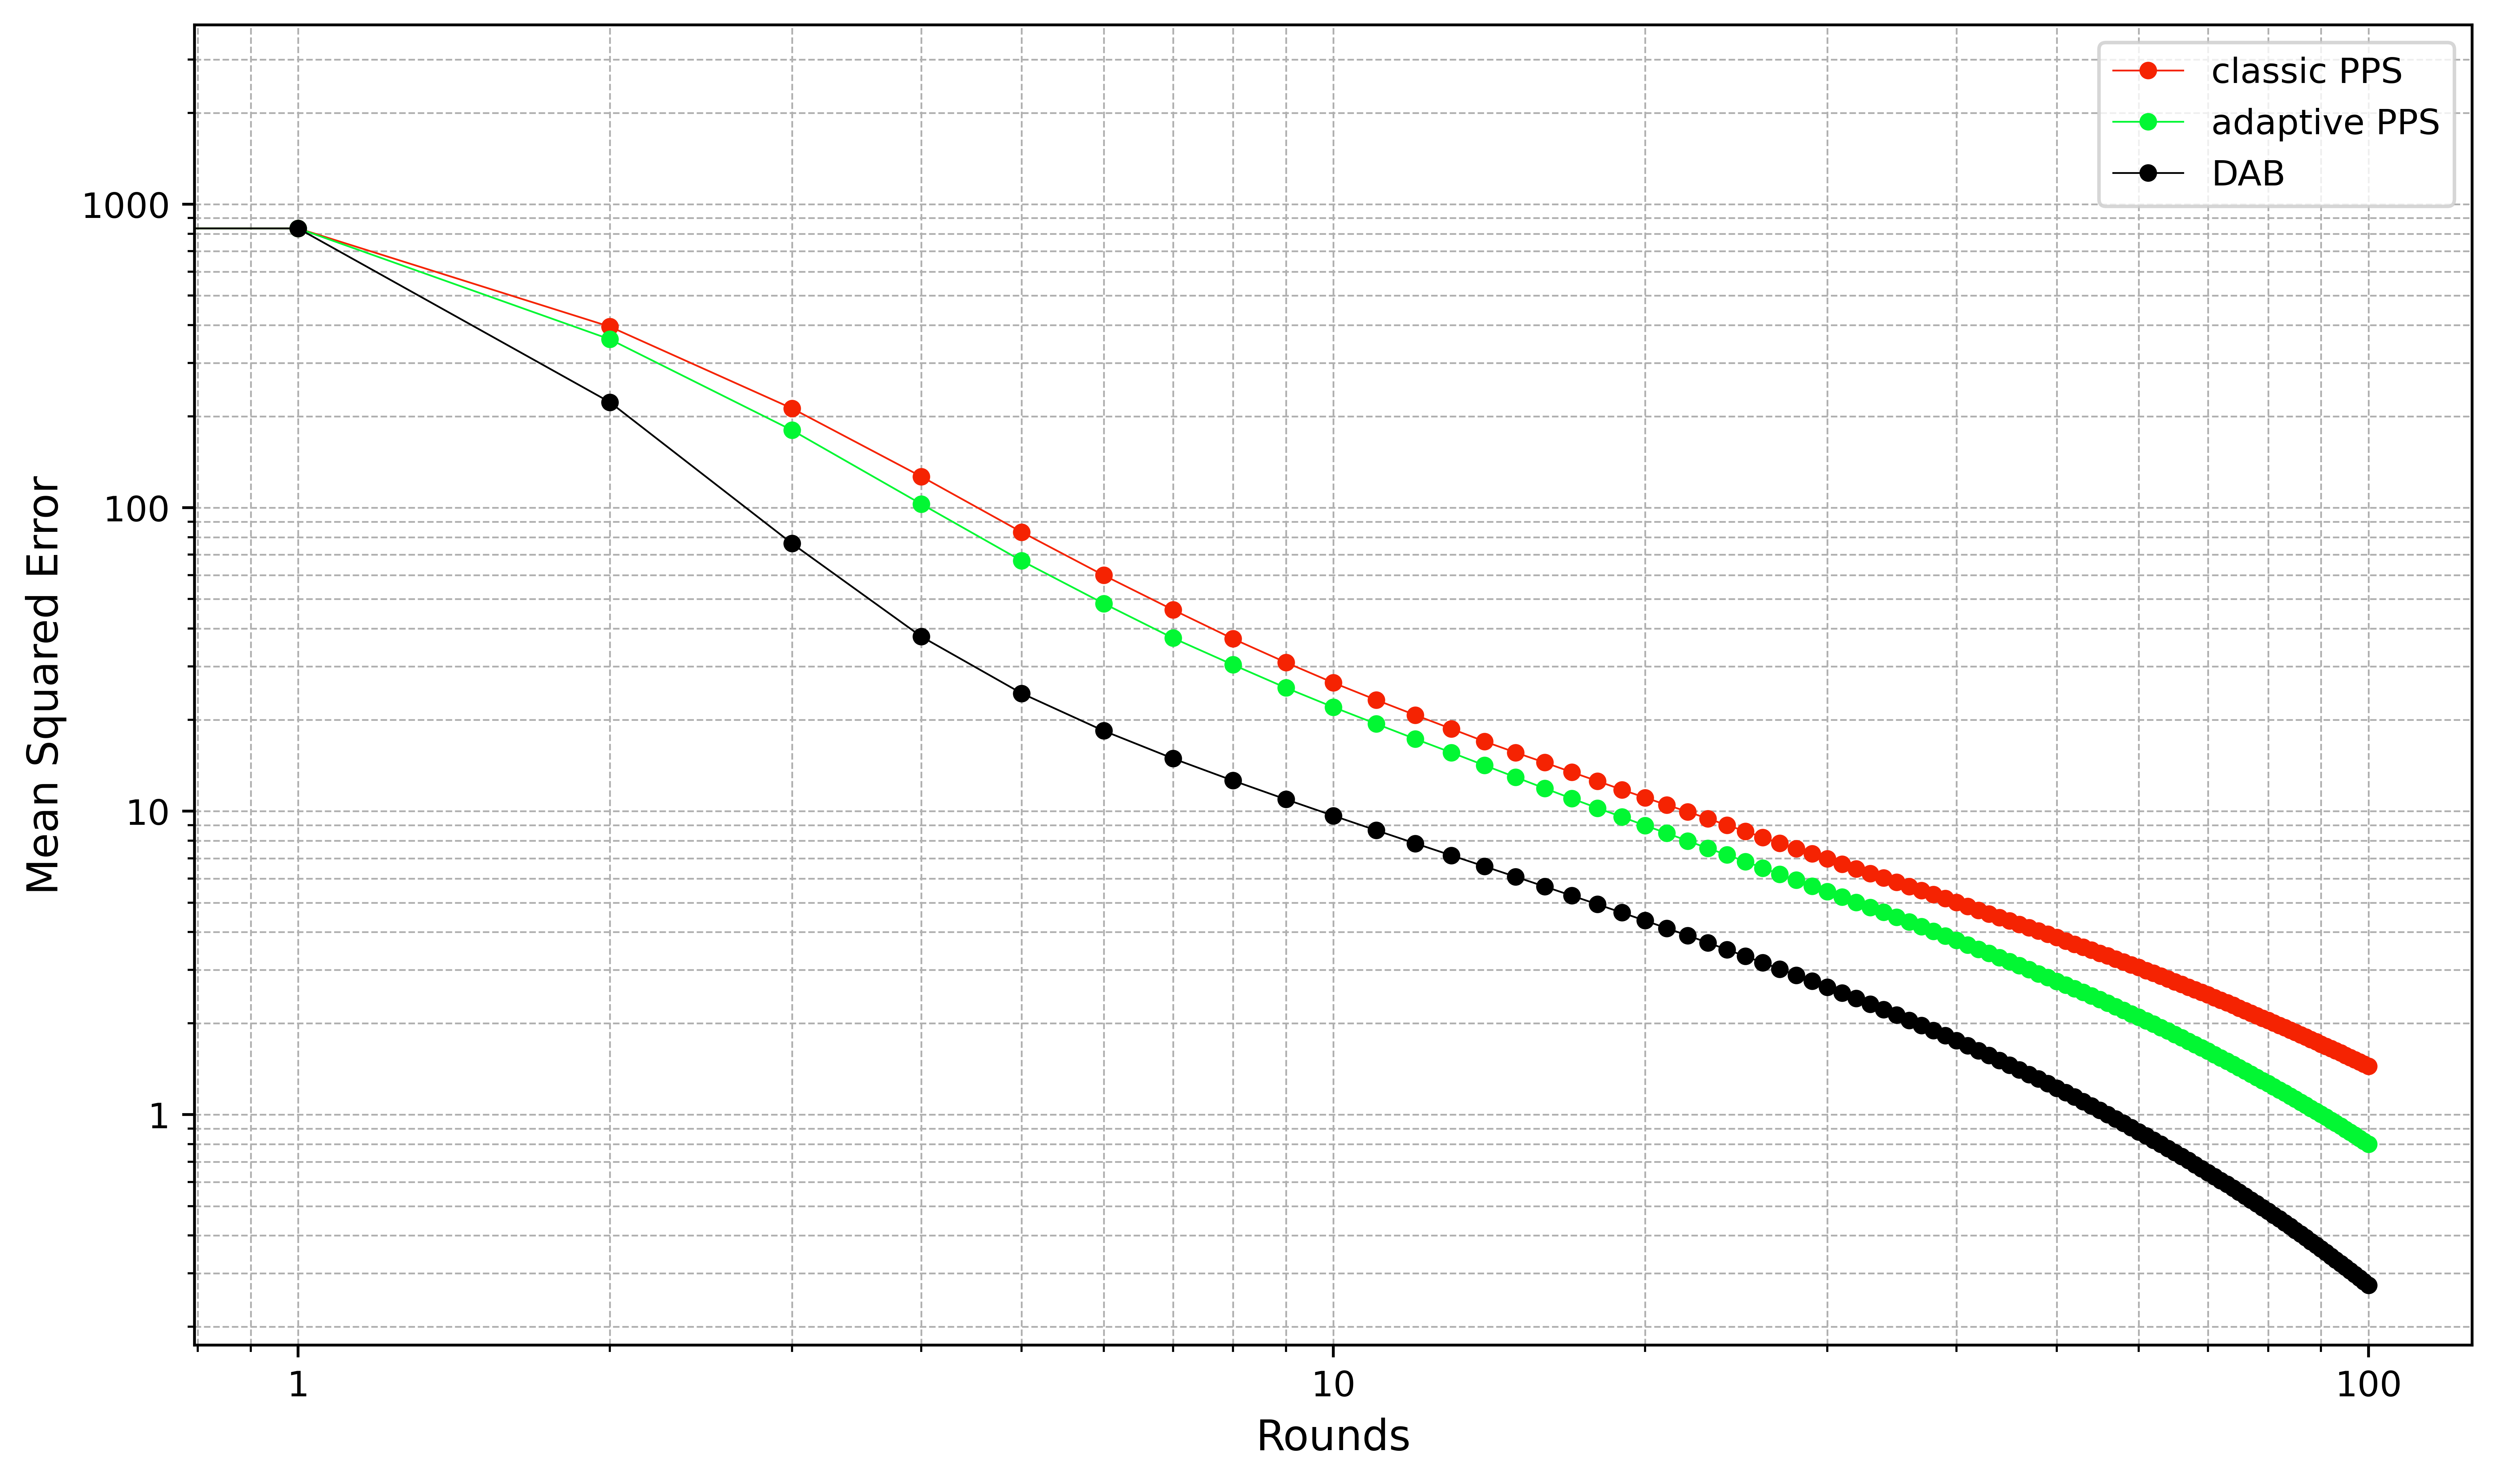
\includegraphics[width=\linewidth]{figures/Simulation_outcomes/TorusGridGraph/DAB_vs_PPS_TGG_r100_n1024_averaged_loglog.png}
    \caption{Torus Grid: mean squared error per rounds (log-log)}
    \label{fig:torusMSEperRoundLogLog}
\end{figure}
\begin{figure}[!ht]
     \centering
         \subfloat[]{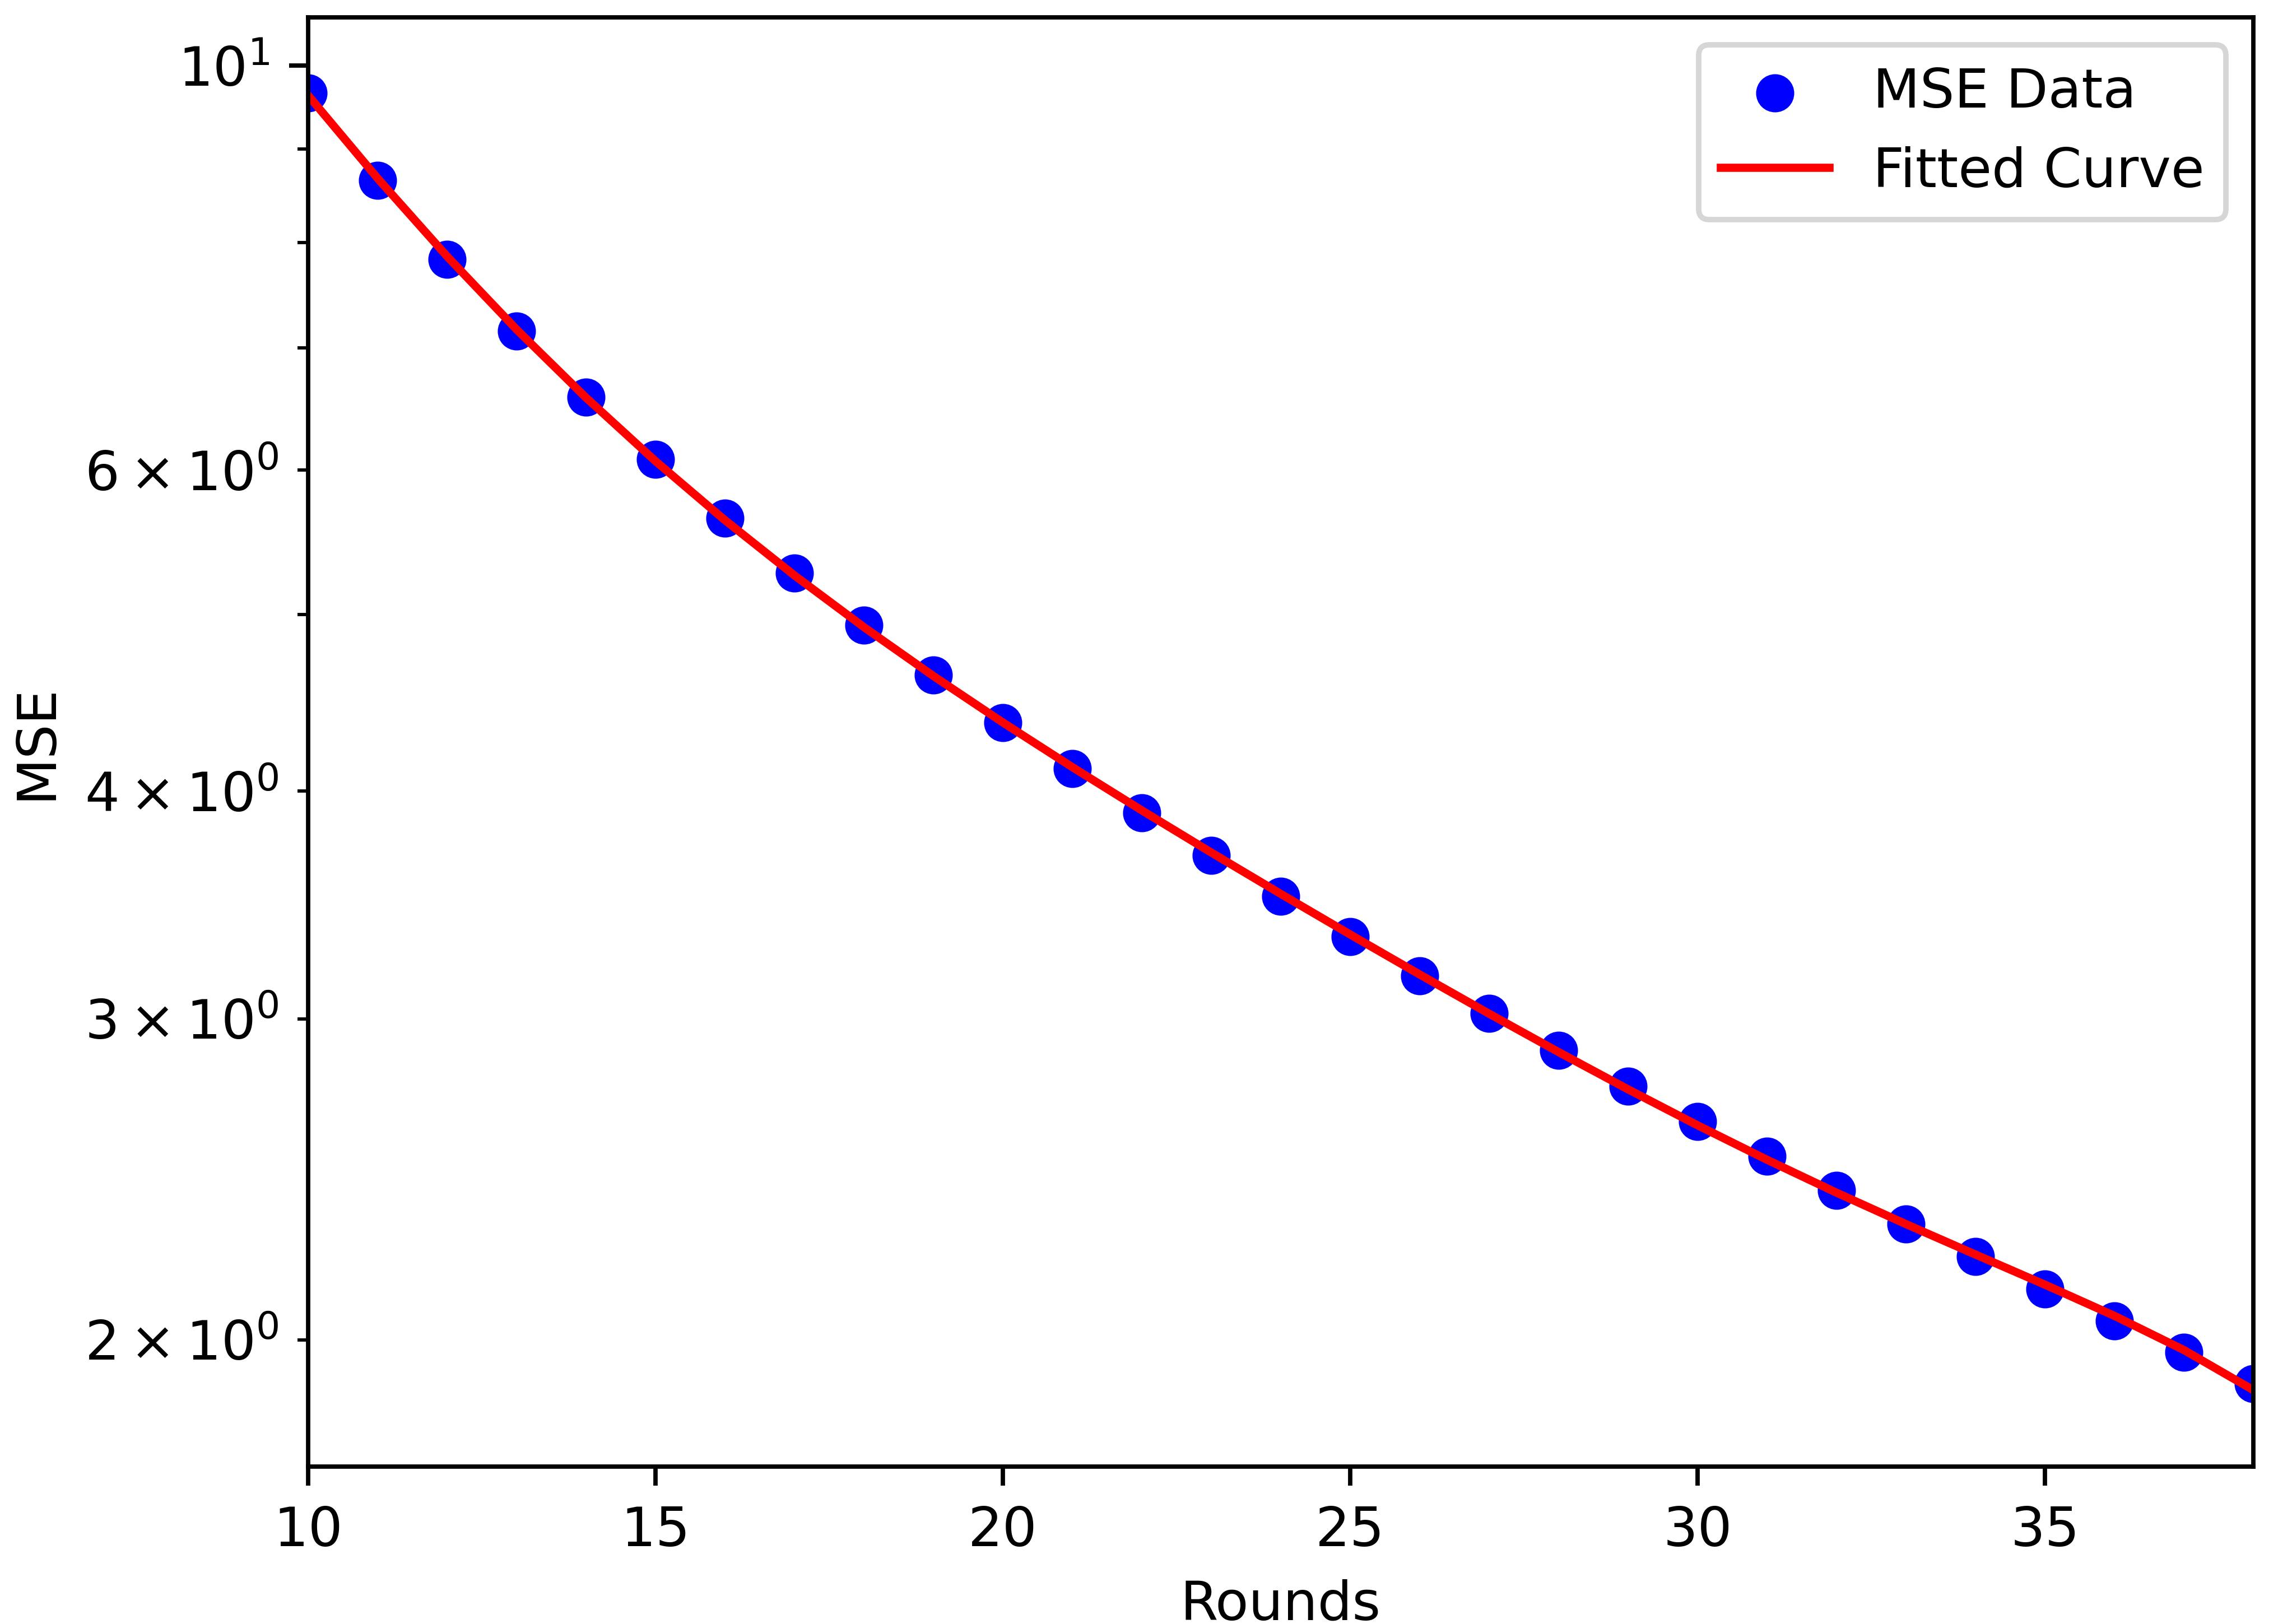
\includegraphics[width=0.49\linewidth]{figures/Simulation_outcomes/TorusGridGraph/DAB/DAB_modelfitting_rounds_38_model_2.png}}
     \hfil
         \subfloat[]{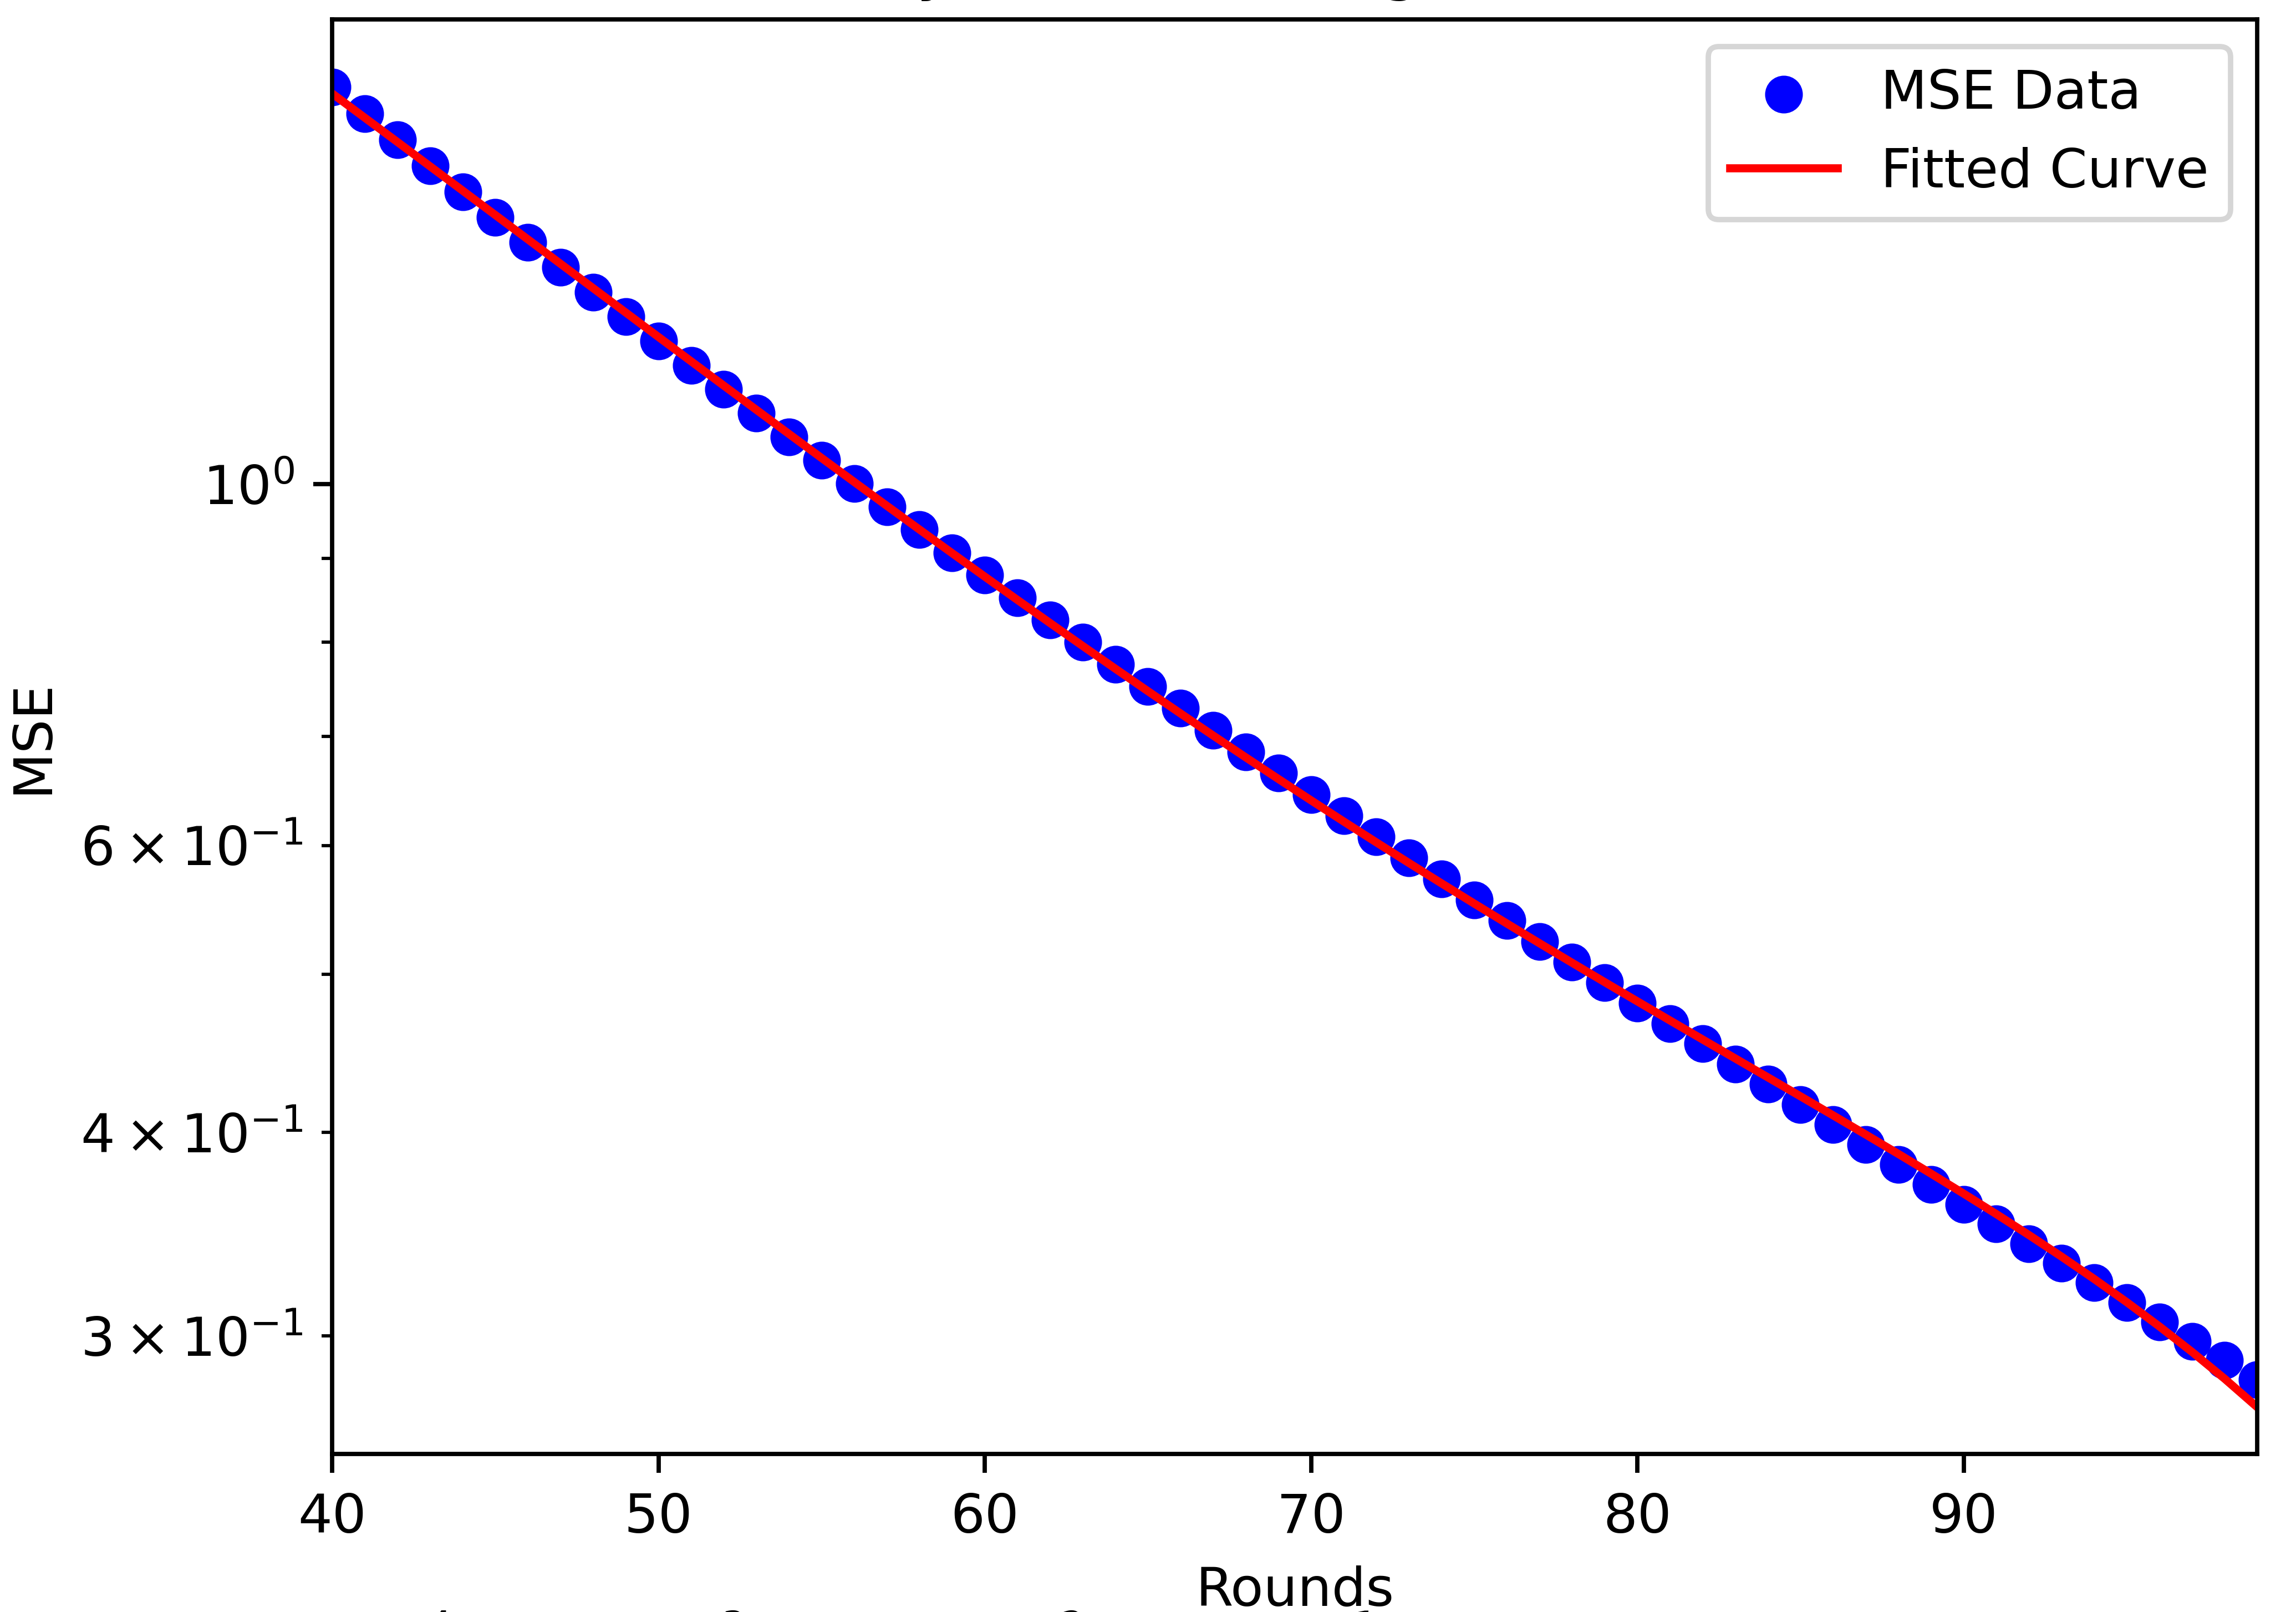
\includegraphics[width=0.49\linewidth]{figures/Simulation_outcomes/TorusGridGraph/DAB/DAB_modelfitting_rounds_99_model_2.png}}
     \caption{Torus Grid - polynomial regression fit: DAB; rounds 10-39 and 40-100}
         \label{fig:dabTorusModelFit}
 \end{figure}
 \begin{figure}[!ht]
     \centering
         \subfloat[]{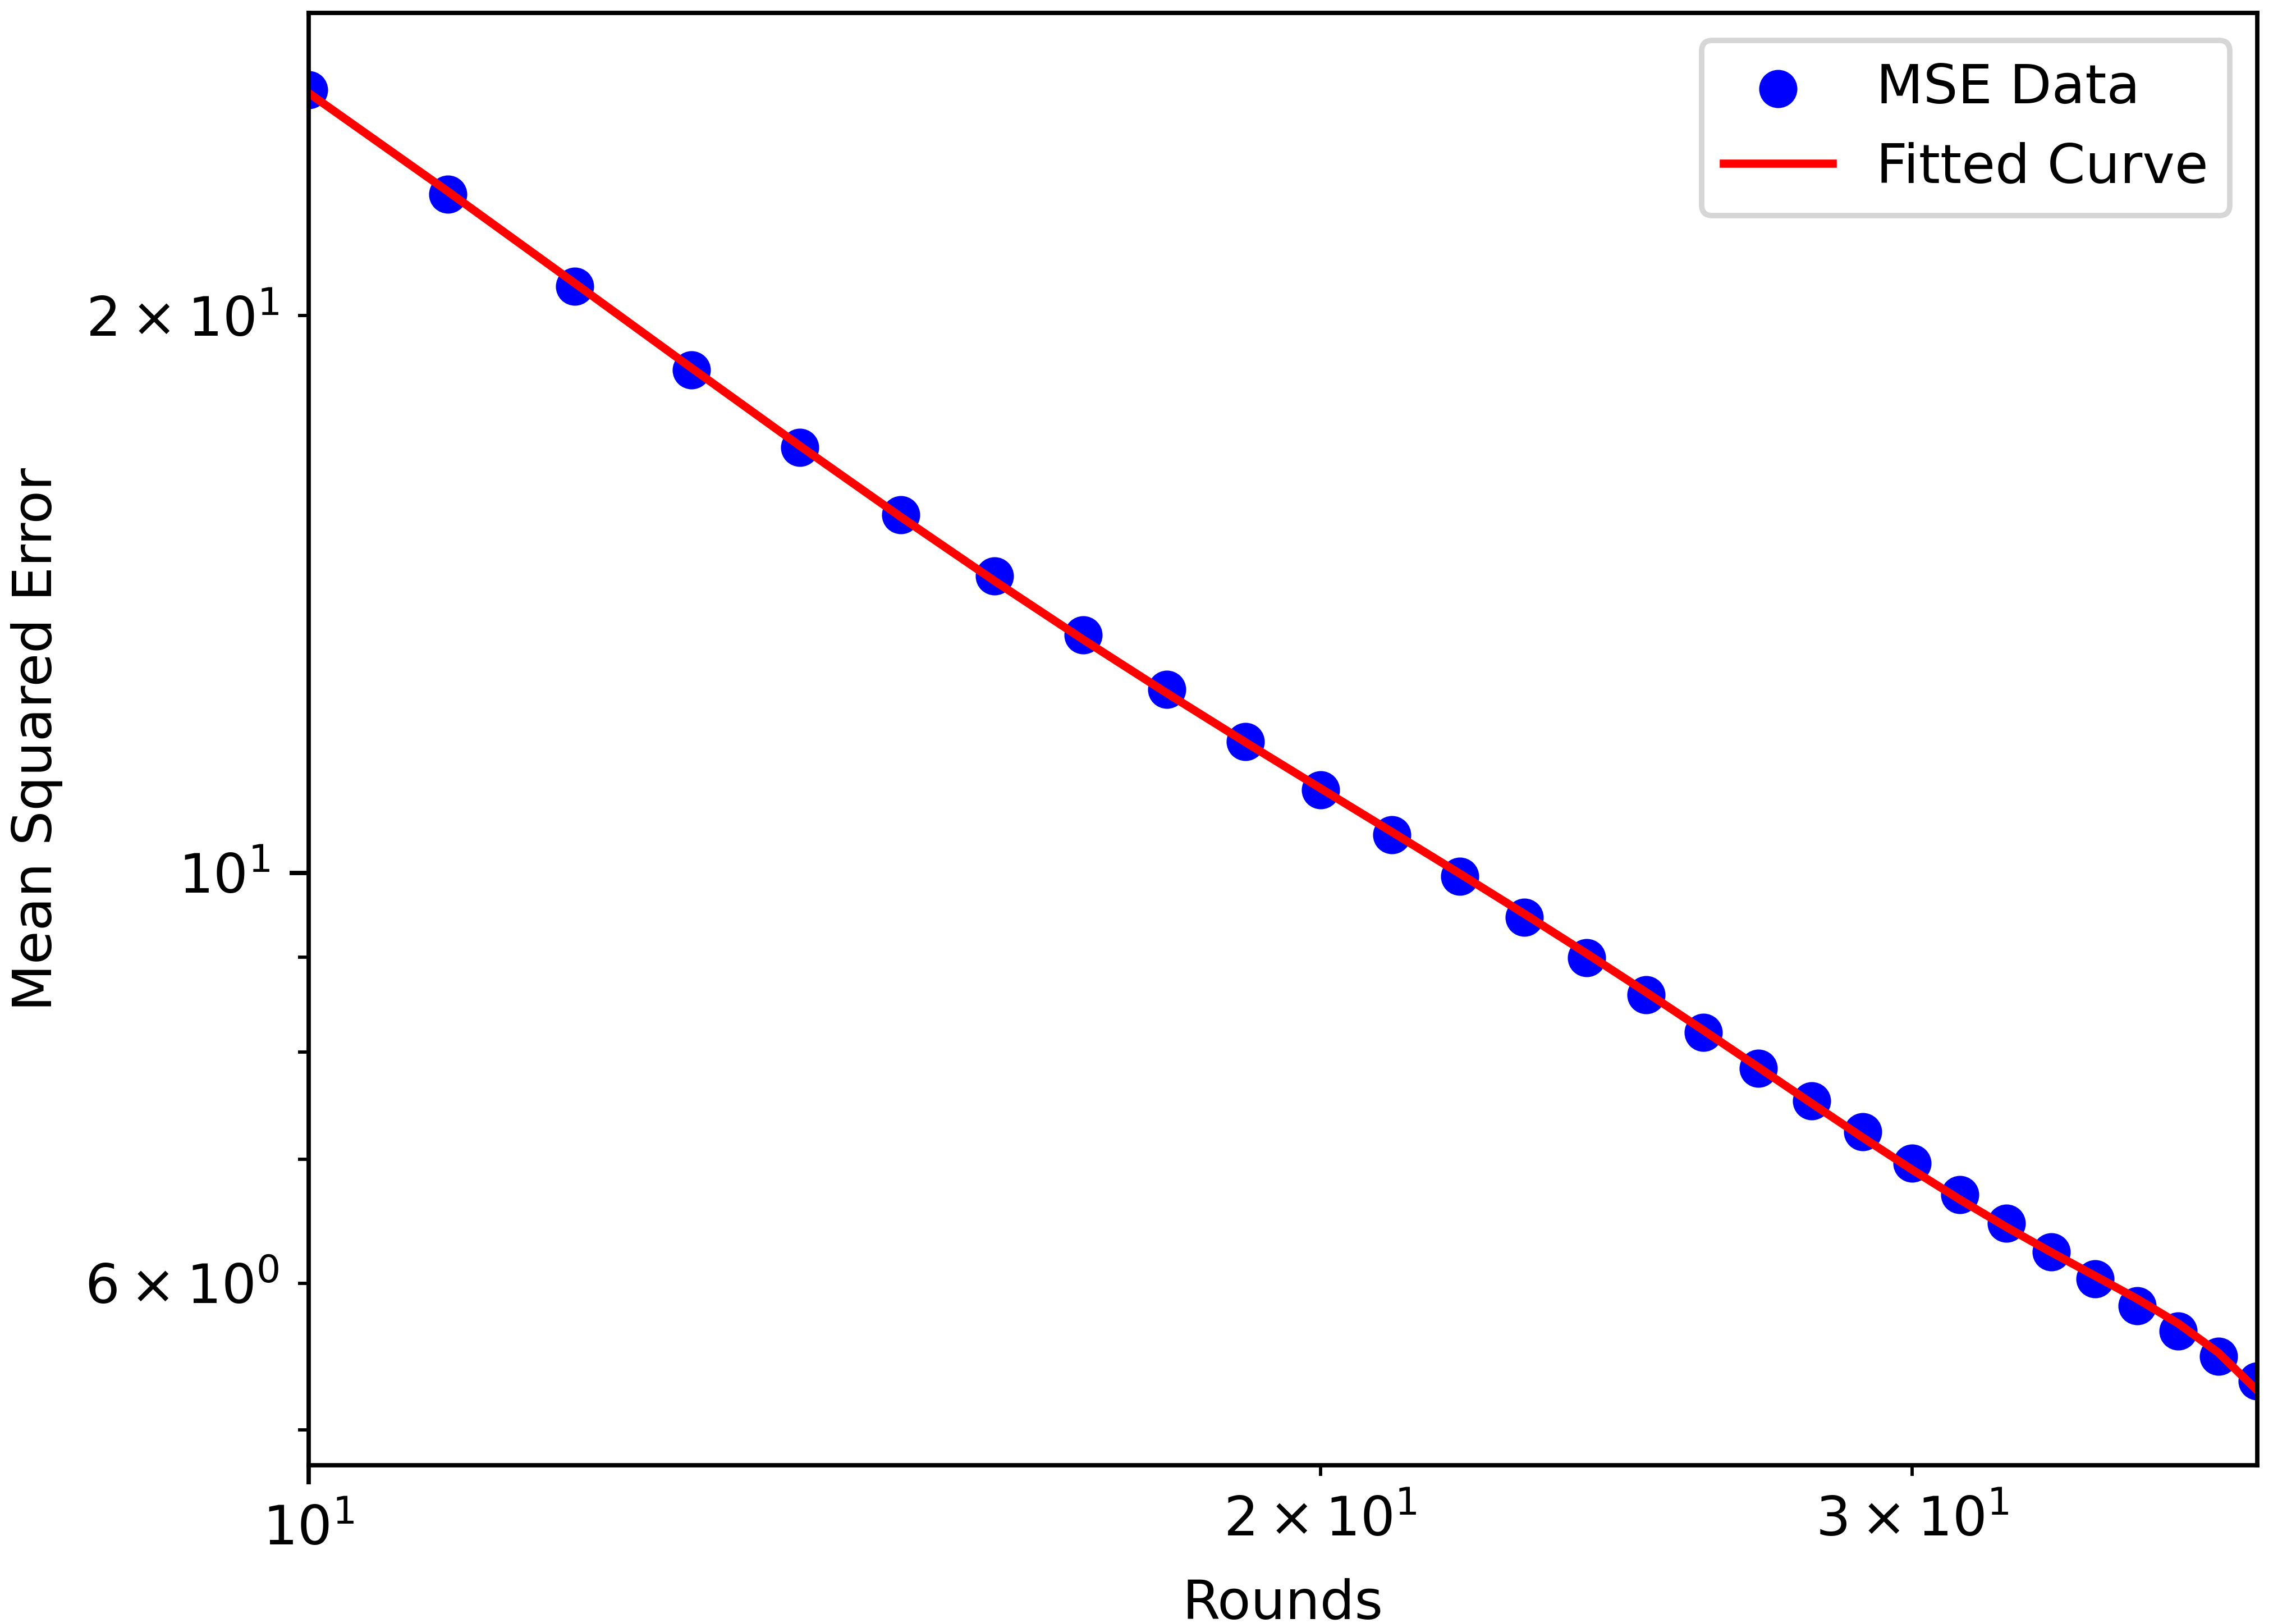
\includegraphics[width=0.49\linewidth]{figures/Simulation_outcomes/TorusGridGraph/PPS/PPS_modelfitting_rounds_38_model_2.png}}
     \hfil
         \subfloat[]{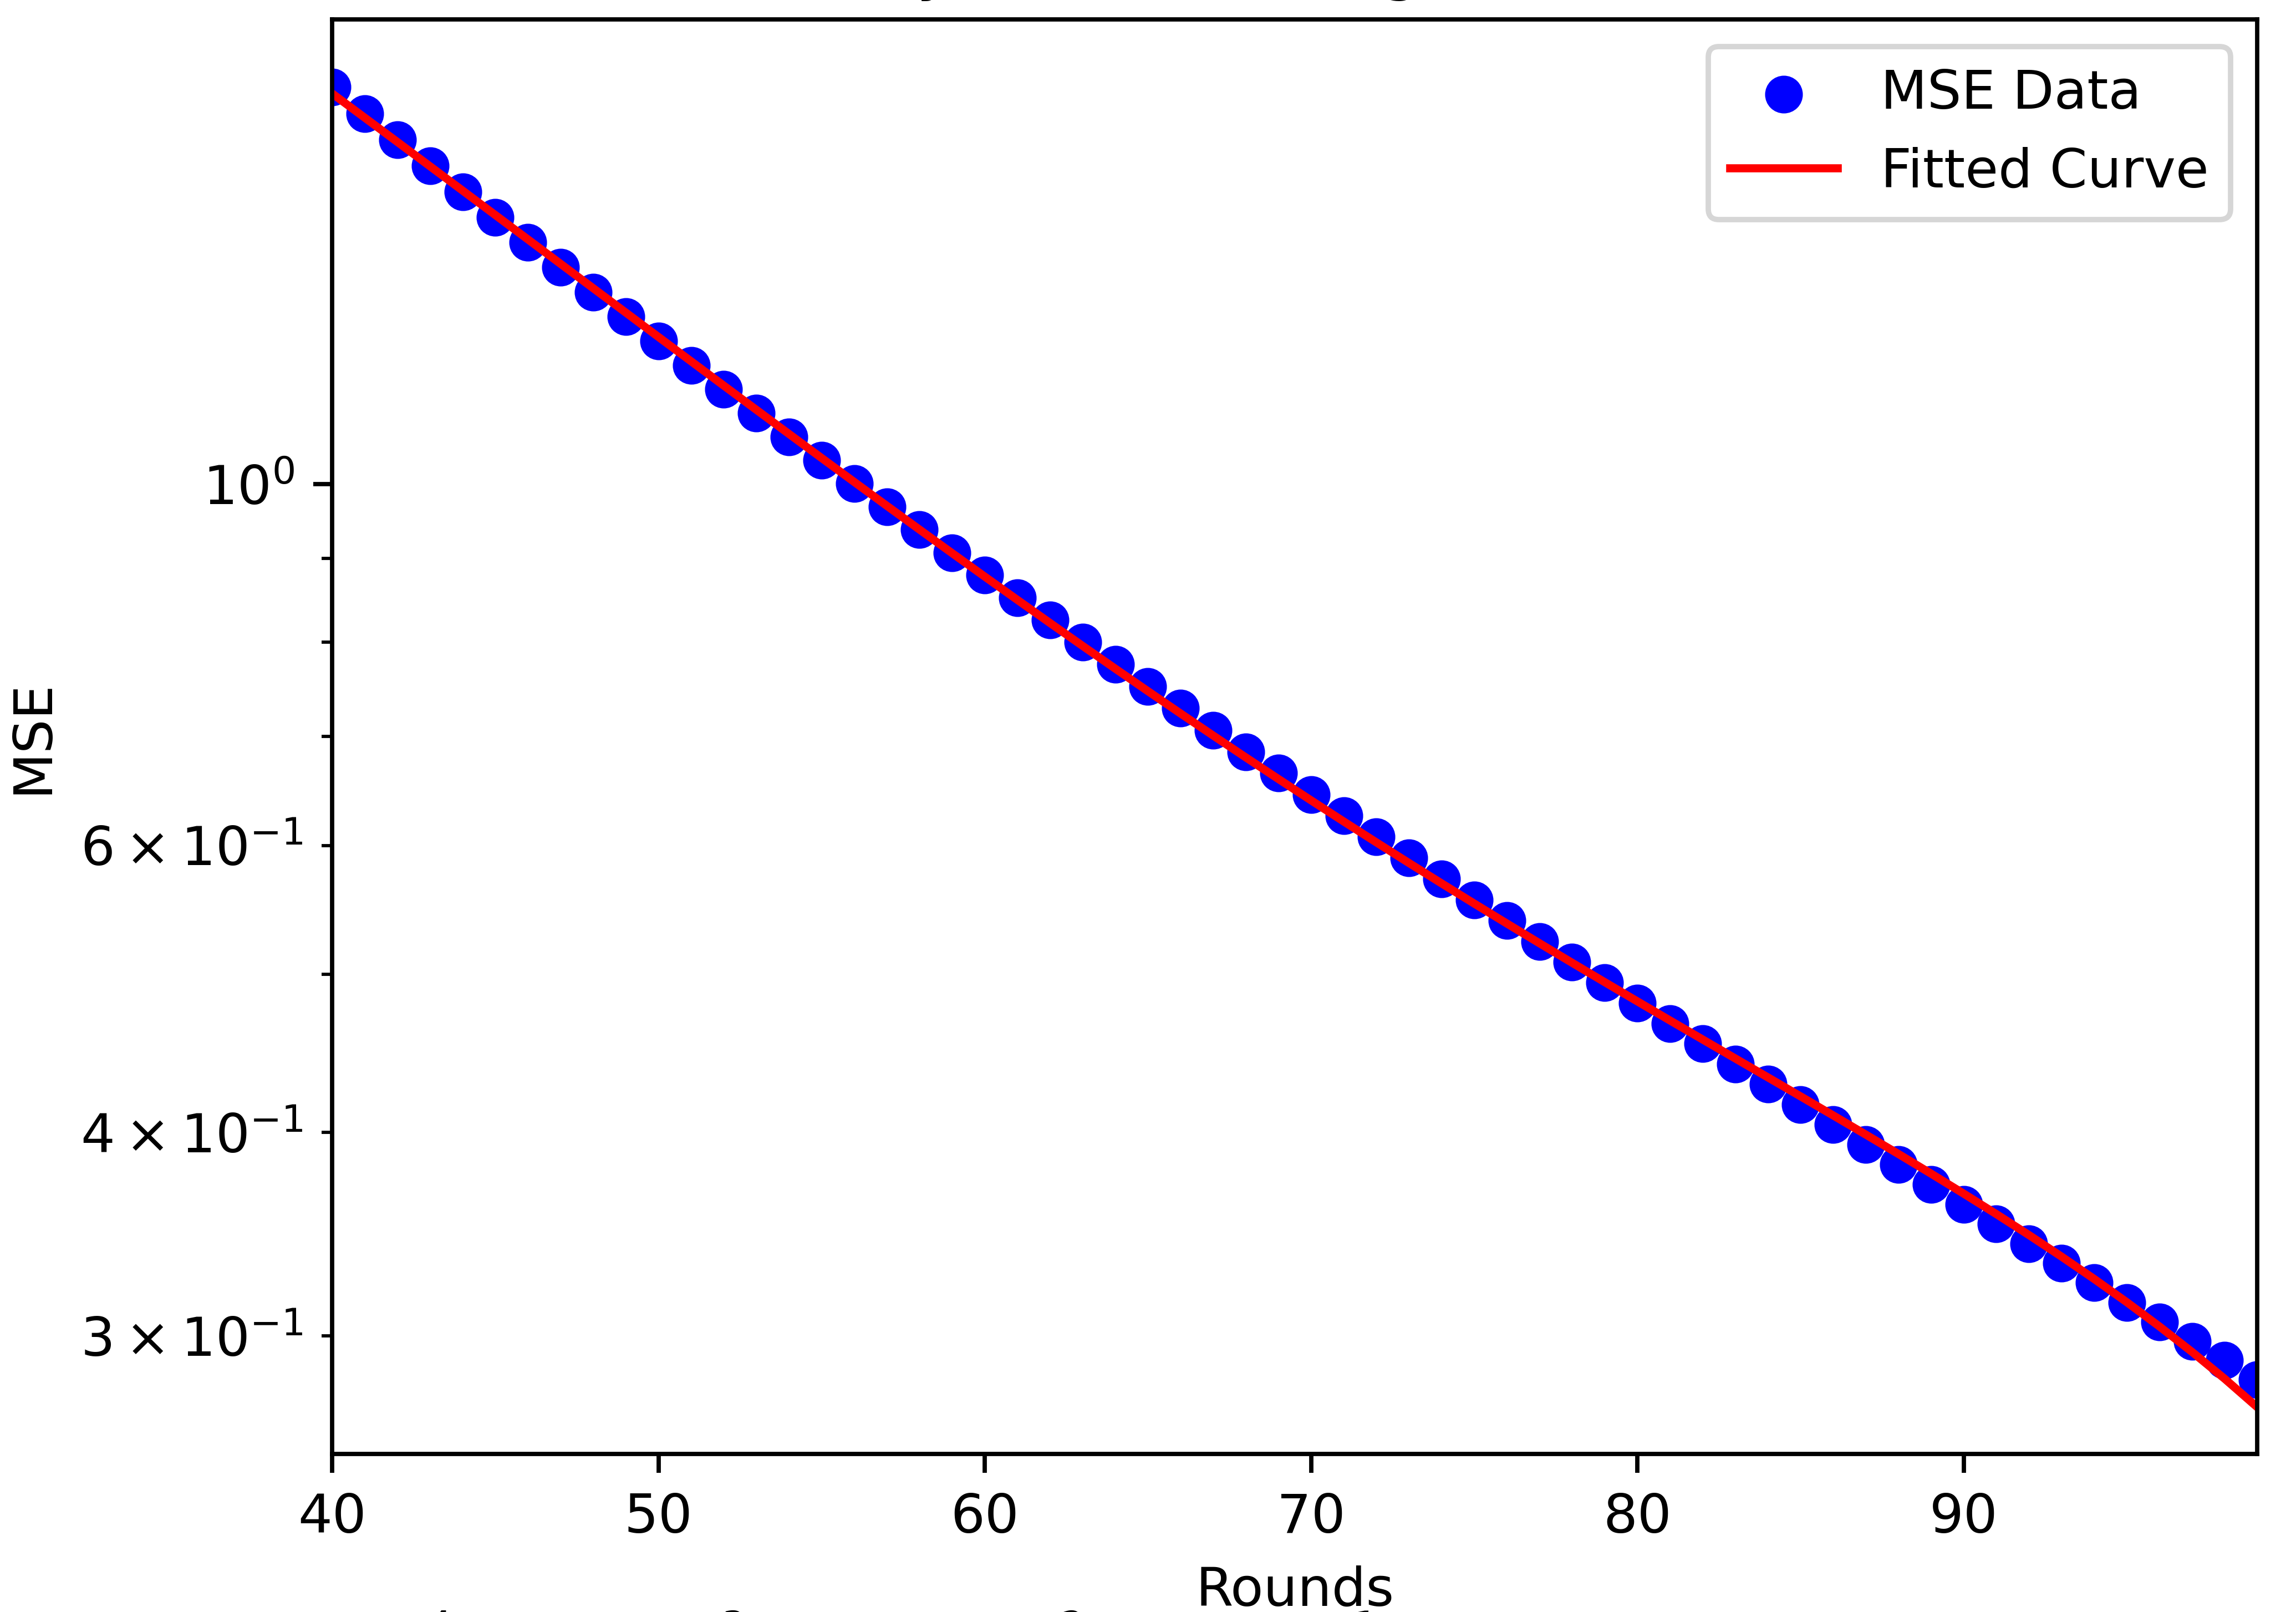
\includegraphics[width=0.49\linewidth]{figures/Simulation_outcomes/TorusGridGraph/DAB/DAB_modelfitting_rounds_99_model_2.png}}
     \caption{Torus Grid - polynomial regression fit: PPS; rounds 10-39 and 40-100}
         \label{fig:ppsTorusModelFit}
 \end{figure}
\begin{figure}[!ht]
    \centering
        \subfloat[]{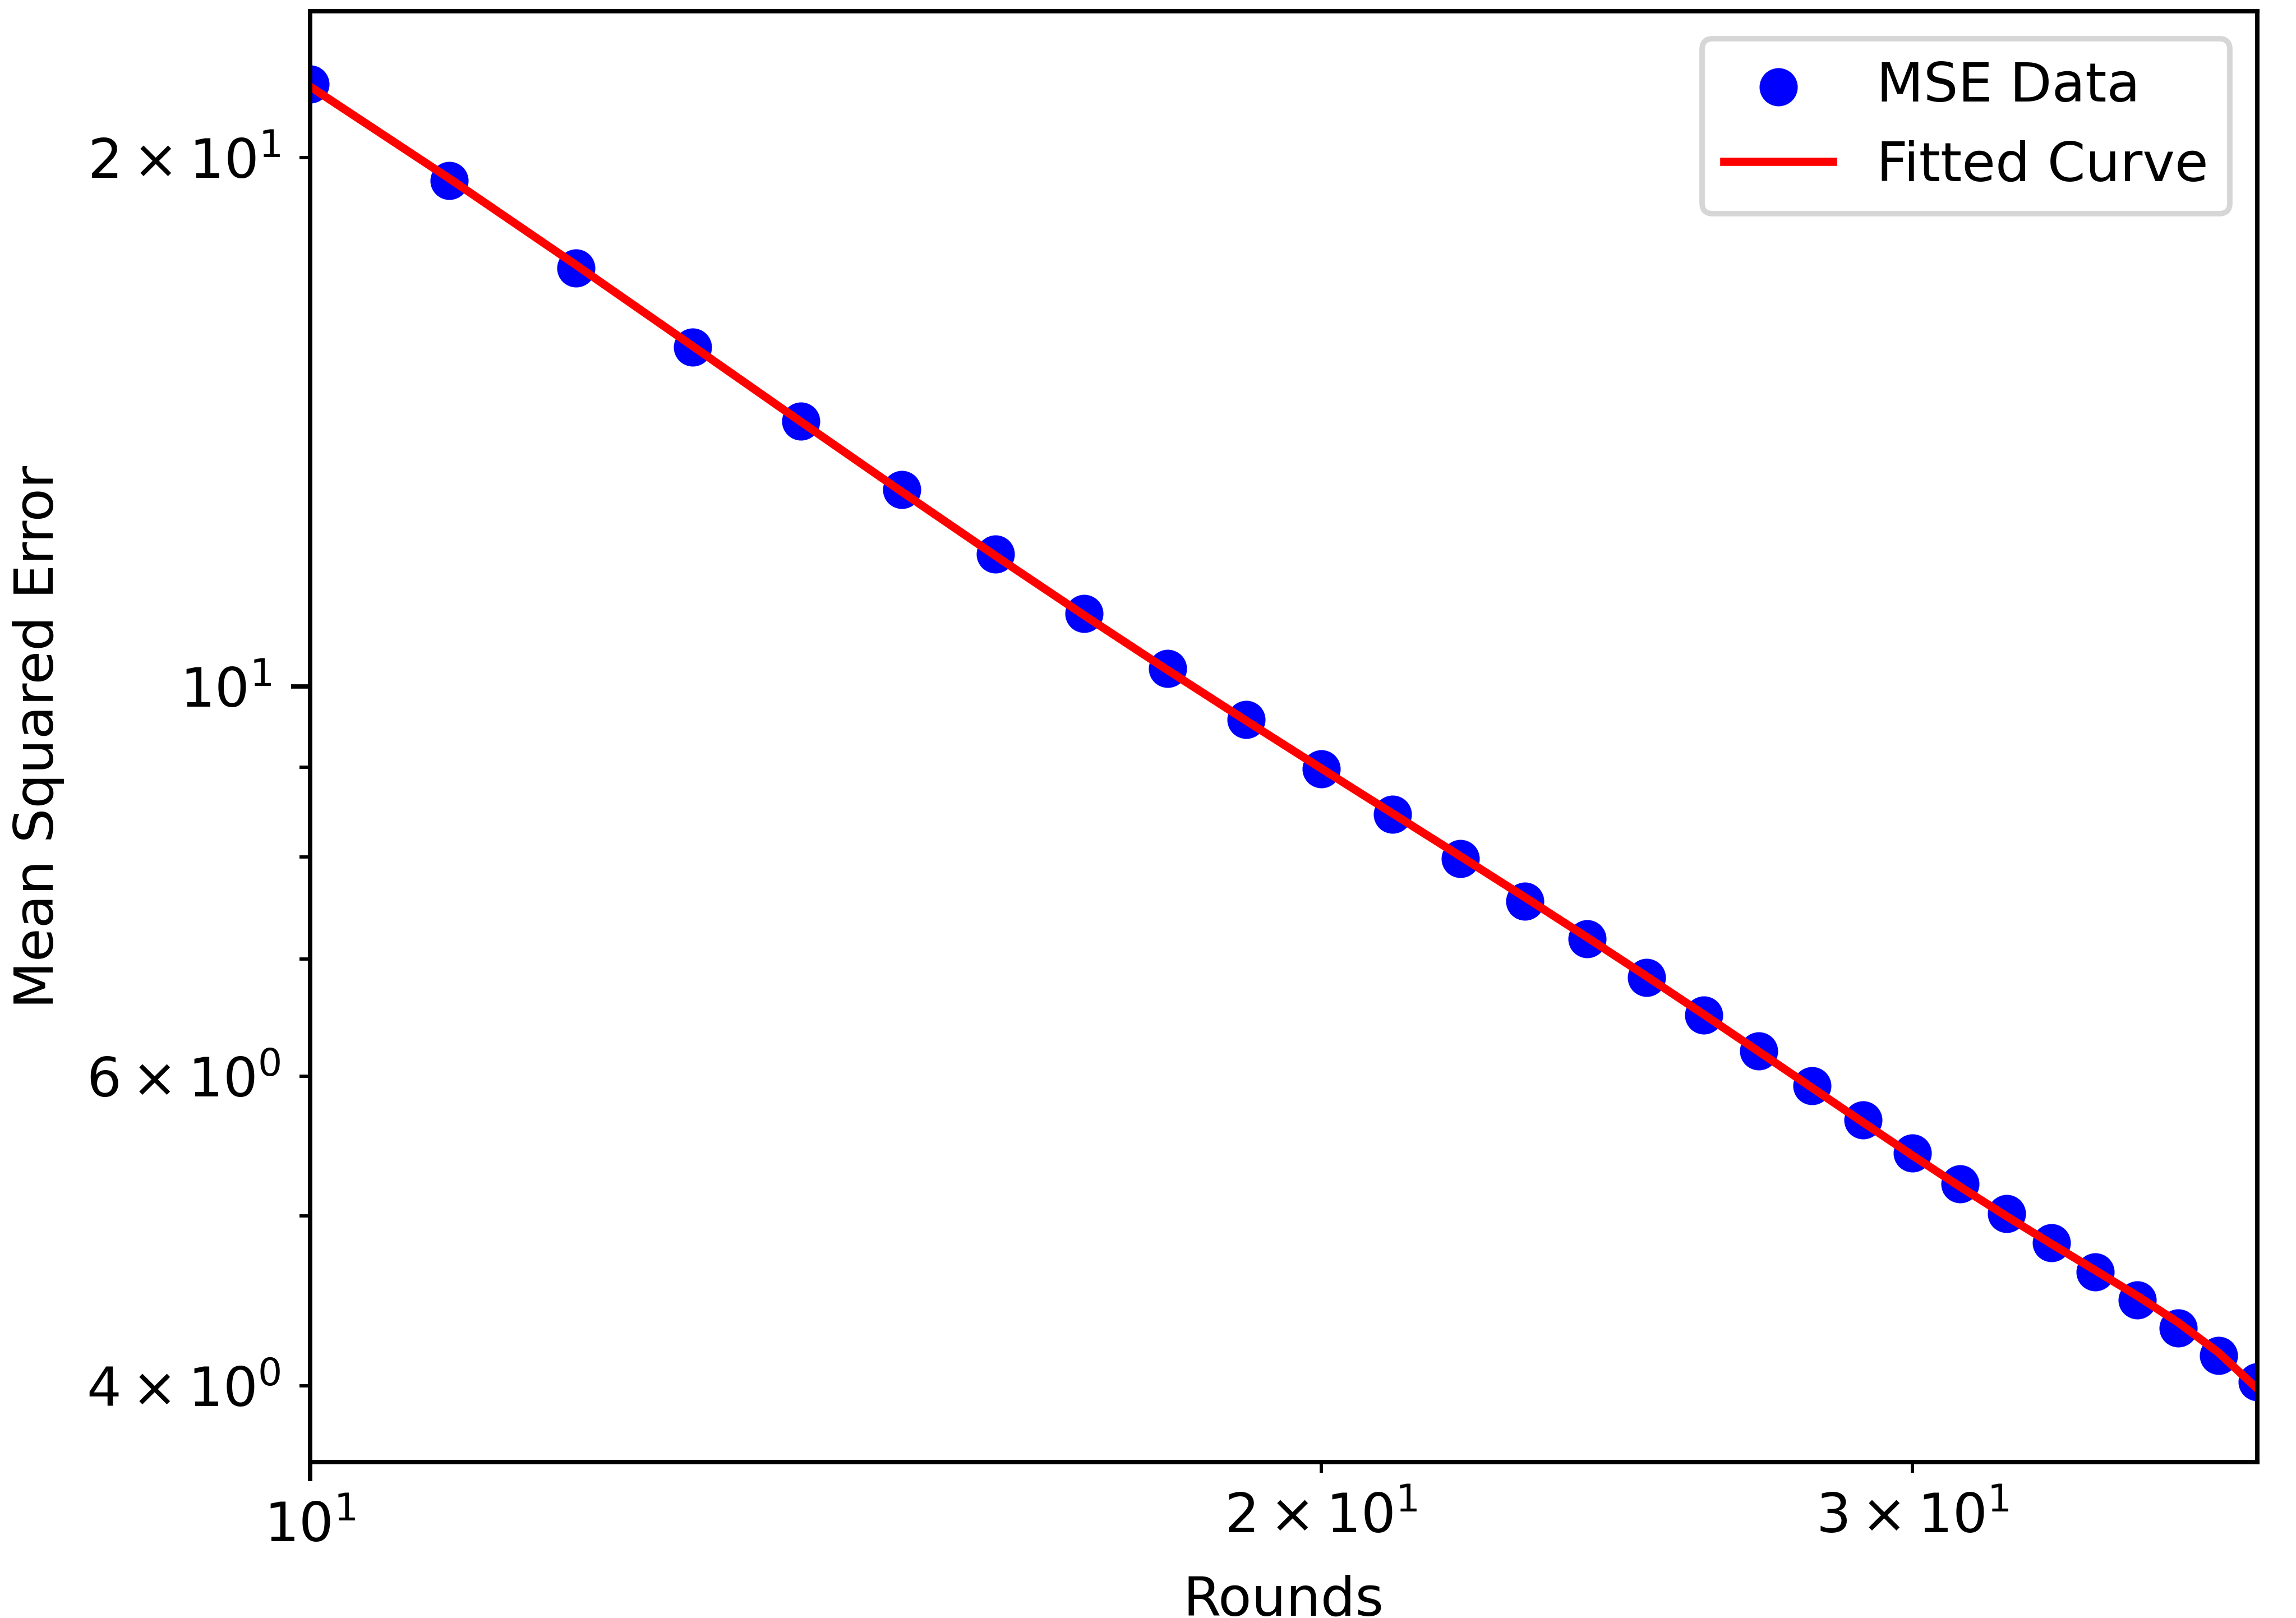
\includegraphics[width=0.49\linewidth]{figures/Simulation_outcomes/TorusGridGraph/ATPPS/ATPPS_modelfitting_rounds_38_model_2.png}}
    \hfil
        \subfloat[]{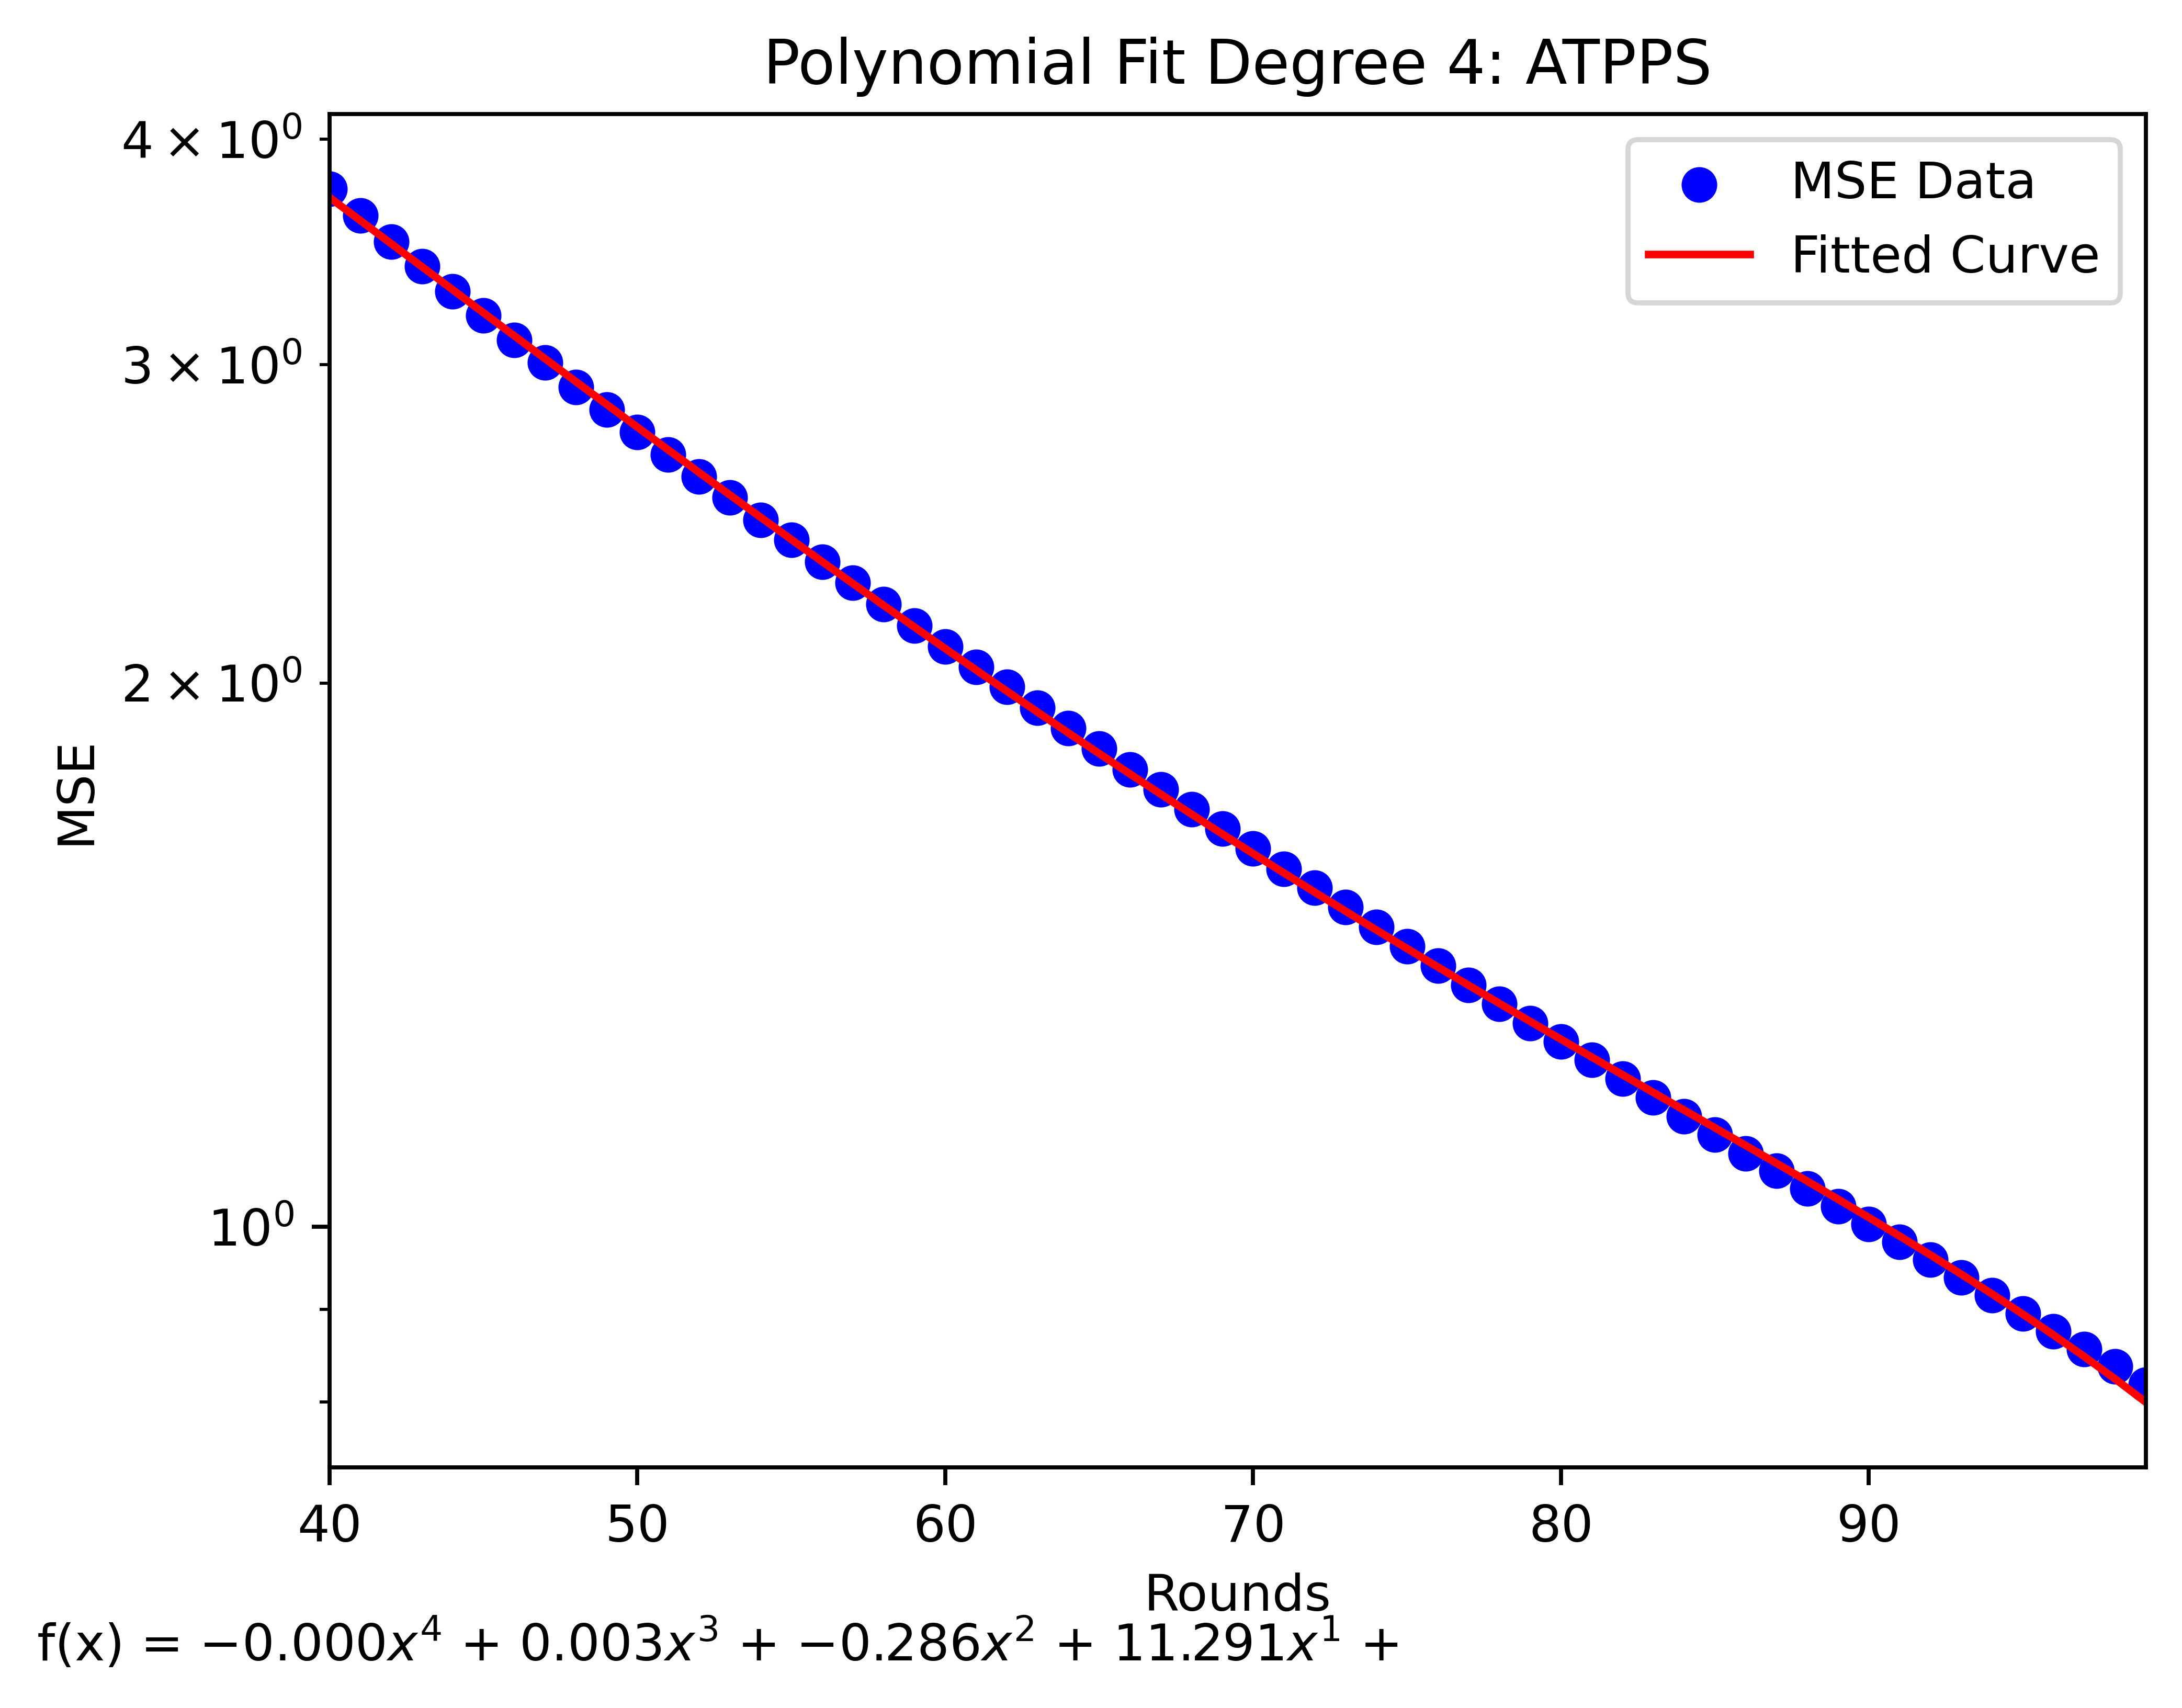
\includegraphics[width=0.49\linewidth]{figures/Simulation_outcomes/TorusGridGraph/ATPPS/ATPPS_modelfitting_rounds_99_model_2.png}}
    \caption{Torus Grid - polynomial regression fit: ATPPS; rounds 10-39 and 40-100}
        \label{fig:atppstorusModelFit}
\end{figure}
 \begin{figure}
     \centering
     \scalebox{0.8}{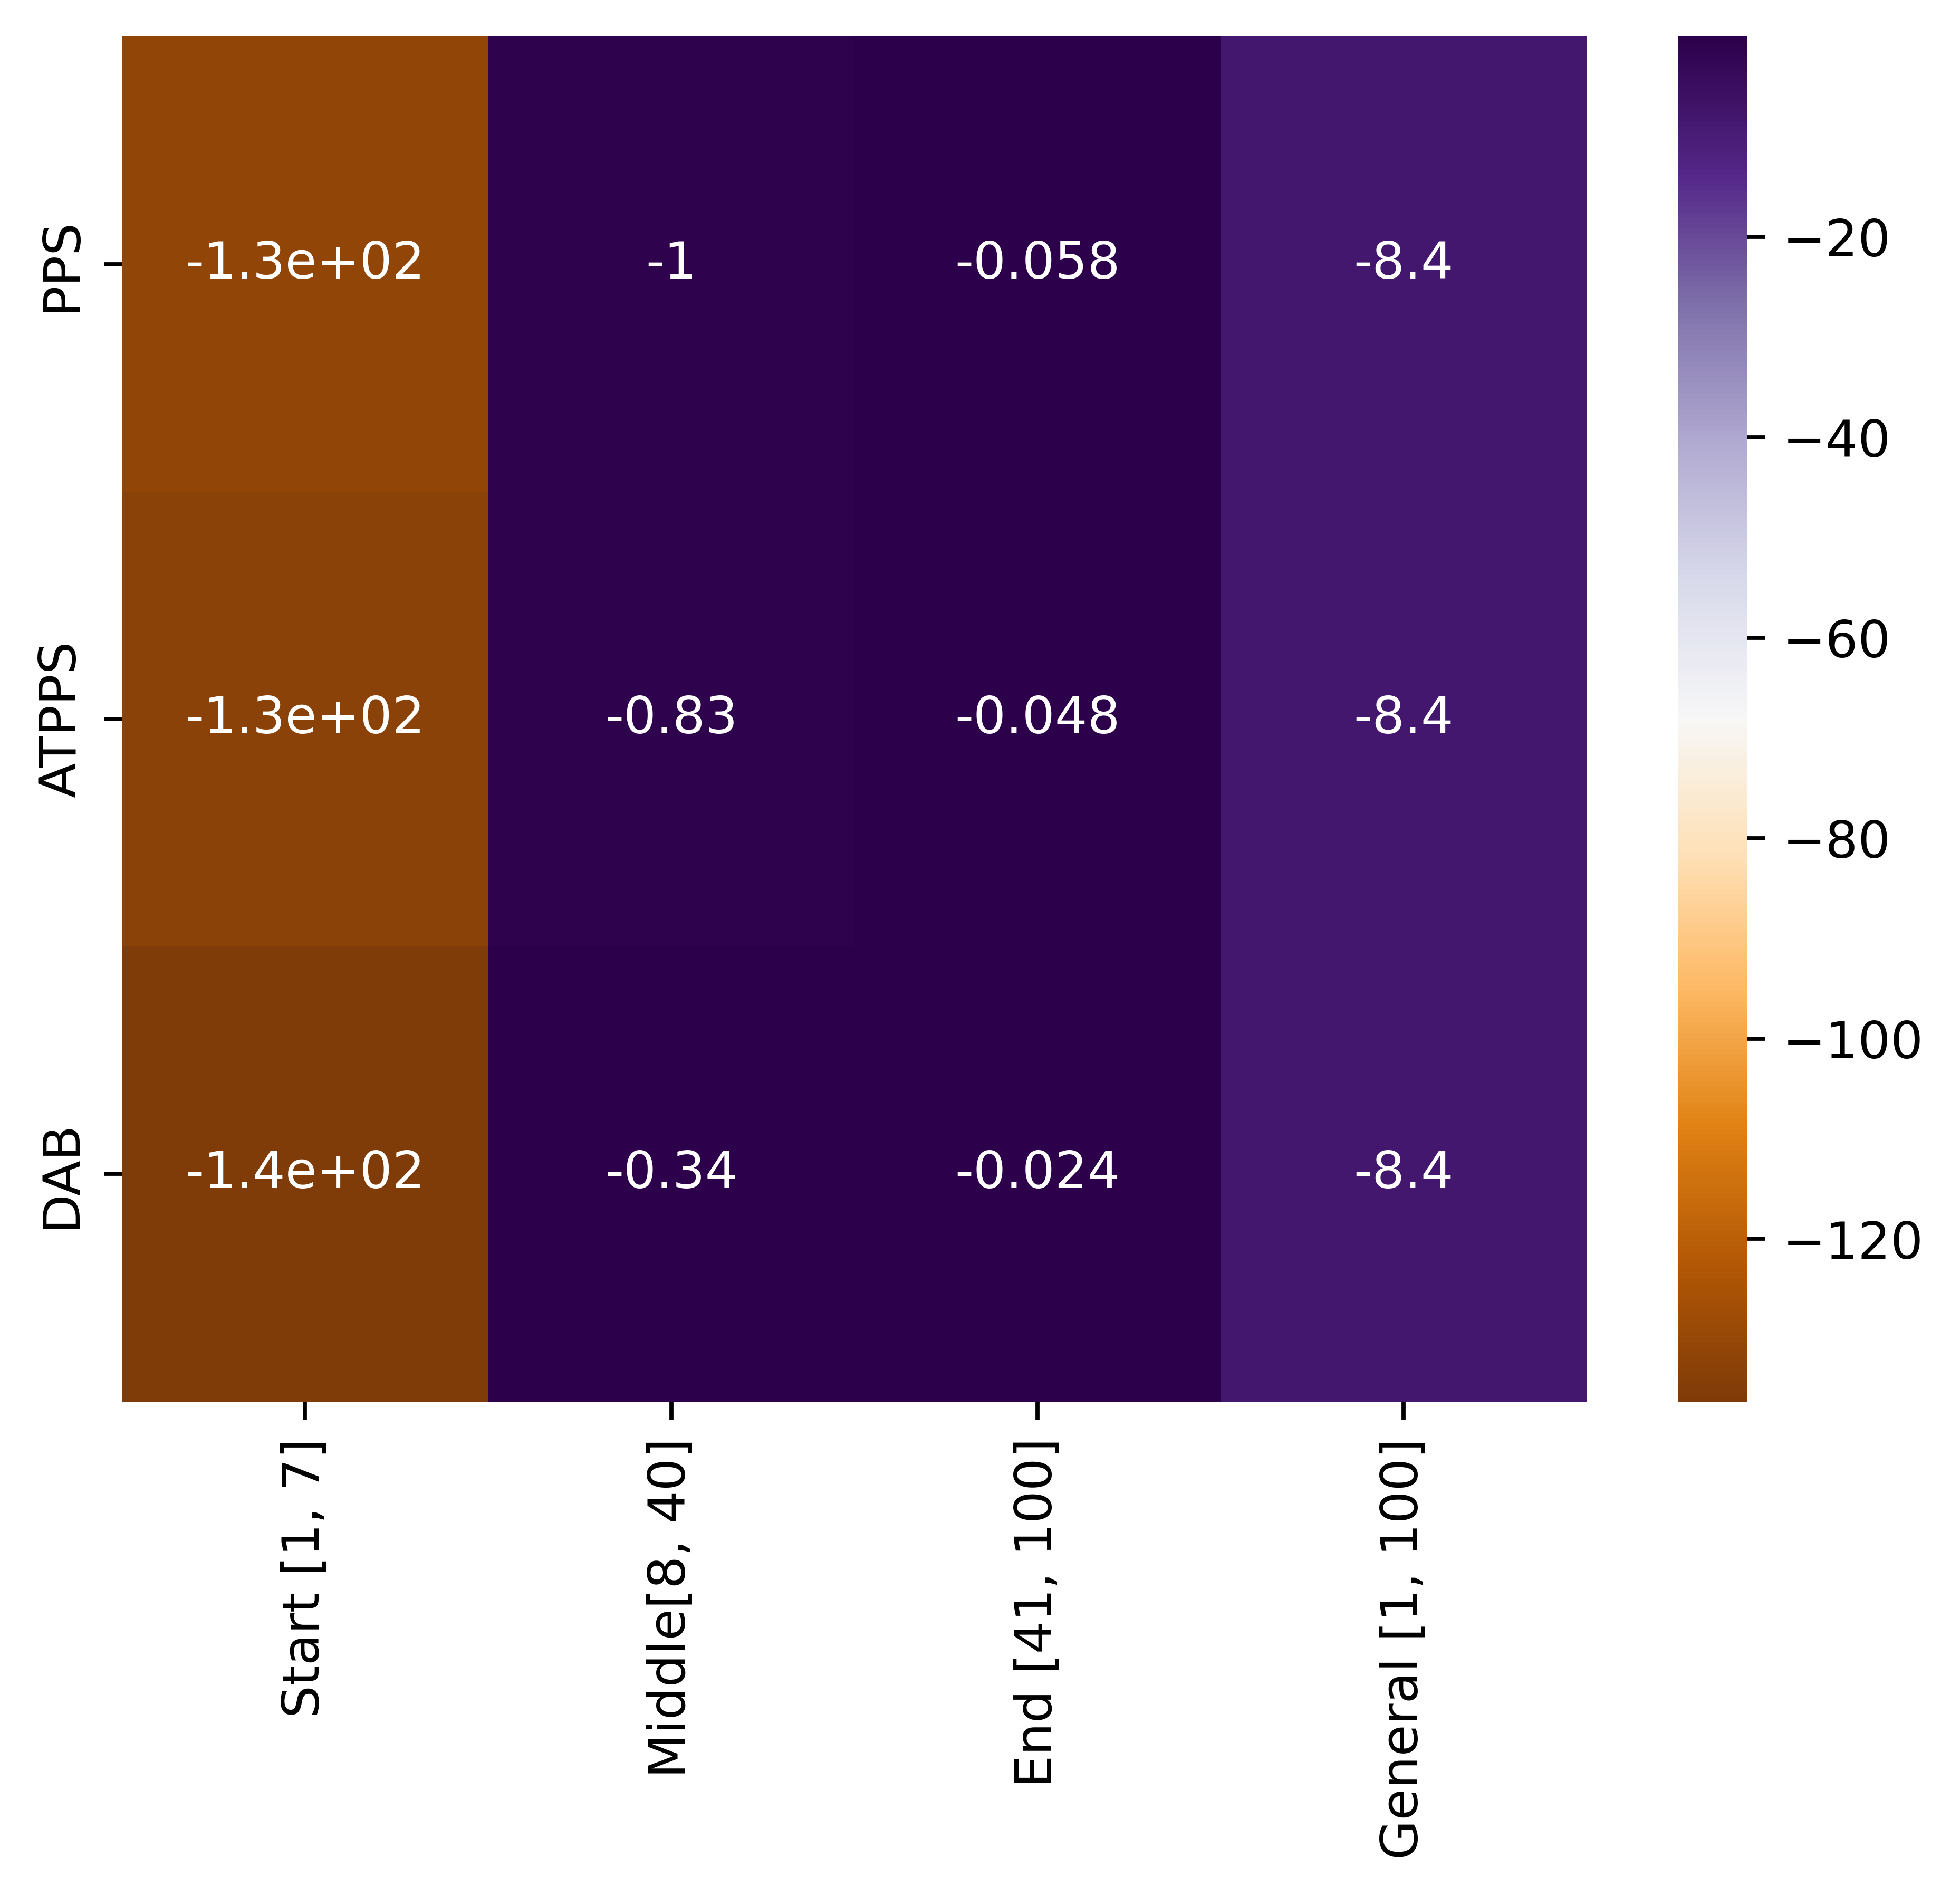
\includegraphics{figures/Simulation_outcomes/TorusGridGraph/DAB_vs_PPS_vs_ATPPS_slopesheatmap_100rounds.png}}
     \caption{Torus Grid: heat map of slopes per region}
     \label{fig:torusgraphslopes}
 \end{figure}

 \section{Lollipop Graph}\label{sec:lollipopgraph}
\subsection{(512, 512) Lollipop Graph}
Figure \ref{fig:lollipopgraphMSEperRoundLogLog} displays the three curves of the load balancing algorithms. The ATPPS slightly outperforms the PPS. The ATPPS slightly outperforms the PPS, while the DAB algorithm underperforms compared to both Push-Pull Sum-based methods in reducing the error. The superior performance of PPS and ATPPS compared to DAB in the Lollipop graph can be explained by the structure of the graph and the fundamental differences in how these algorithms operate. The clique region is characterized by high connectivity and enables rapid local balancing for the Push-Pull Sum based algorithms. While the path region with limited connectivity slows down information propagation and balancing for the Push-Pull Sum based algorithms and favors the deterministic algorithm DAB. The initial discrepancy in the first 10 rounds arises due to the potentially rapid error reduction achieved by PPS within the clique. The DAB struggles to perform well for cliques, as observed in section \ref{sec:completeGraph}. DAB performs rather well in the Path graph which in theory is similar to the Ring graph without the edge connecting the first and last nodes as described in section \ref{sec:ringgraph}. It prioritizes nodes with the least load, which can lead to inefficient propagation along the clique. Load imbalances in the clique region take longer to converge because DAB does not exploit the random spreading mechanism of Push-Pull Sum based algorithms. In the initial phase, PPS rapidly reduces the MSE, demonstrating strong initial convergence. The Push-Pull Sum based algorithms achieve a steep downward slope with value -130 between rounds 1 and 7, while the DAB reaches nearly half of it with value -67 (figure \ref{fig:lollipopslopes}). In the mid-to-late phase, the slope flattens for both Push-Pull Sum-based algorithms, indicating slower convergence. This is evident from slope values dropping as low as $-0.12$ to $\sim-0.9$. In this phase, the path section of the Lollipop graph dominates the residual imbalances. The ATPPS achieves nearly identical behavior to the PPS in the early rounds, as it starts with similar strategies where the threshold is relatively easy to surpass as the load differences in the network are still very high. ATPPS outperforms the PPS slightly in the later rounds due to its ability to dynamically adjust its balancing strategy based on the current state of load imbalances. This allows it to better address residual imbalances in the path section of the Lollipop graph as showcased in section \ref{sec:ringgraph}.

The MSE data for the DAB algorithm is best described by a polynomial regression model of degree 3, following the equation: $MSE_r=-5.89\times10^{-5}r^{3}+0.03r^{2}-5.68r+459.42$ as shown in figure \ref{fig:dablollipopgraphModelFit}. The MSE trends for the PPS and ATPPS algorithms are better captured by polynomial regression models of degree 4. The best-fit equation for the PPS model is: $MSE_r=8.44\times 10^{-7}r^{4}-2.52\times 10^{-4}r^{3}-0.03r^{2}-1.64r+56.68$ (figure \ref{fig:ppslollipopgraphModelFit}) and the ATPPS model fit follows the equation: $MSE_r=8.69 \times 10^{-7}r^{4}-2.56 \times 10^{-4}r^{3}+0.03r^{2}-1.62r+54.48$ (figure \ref{fig:atppslollipopgraphModelFit}).

\begin{figure}[]
    \centering
    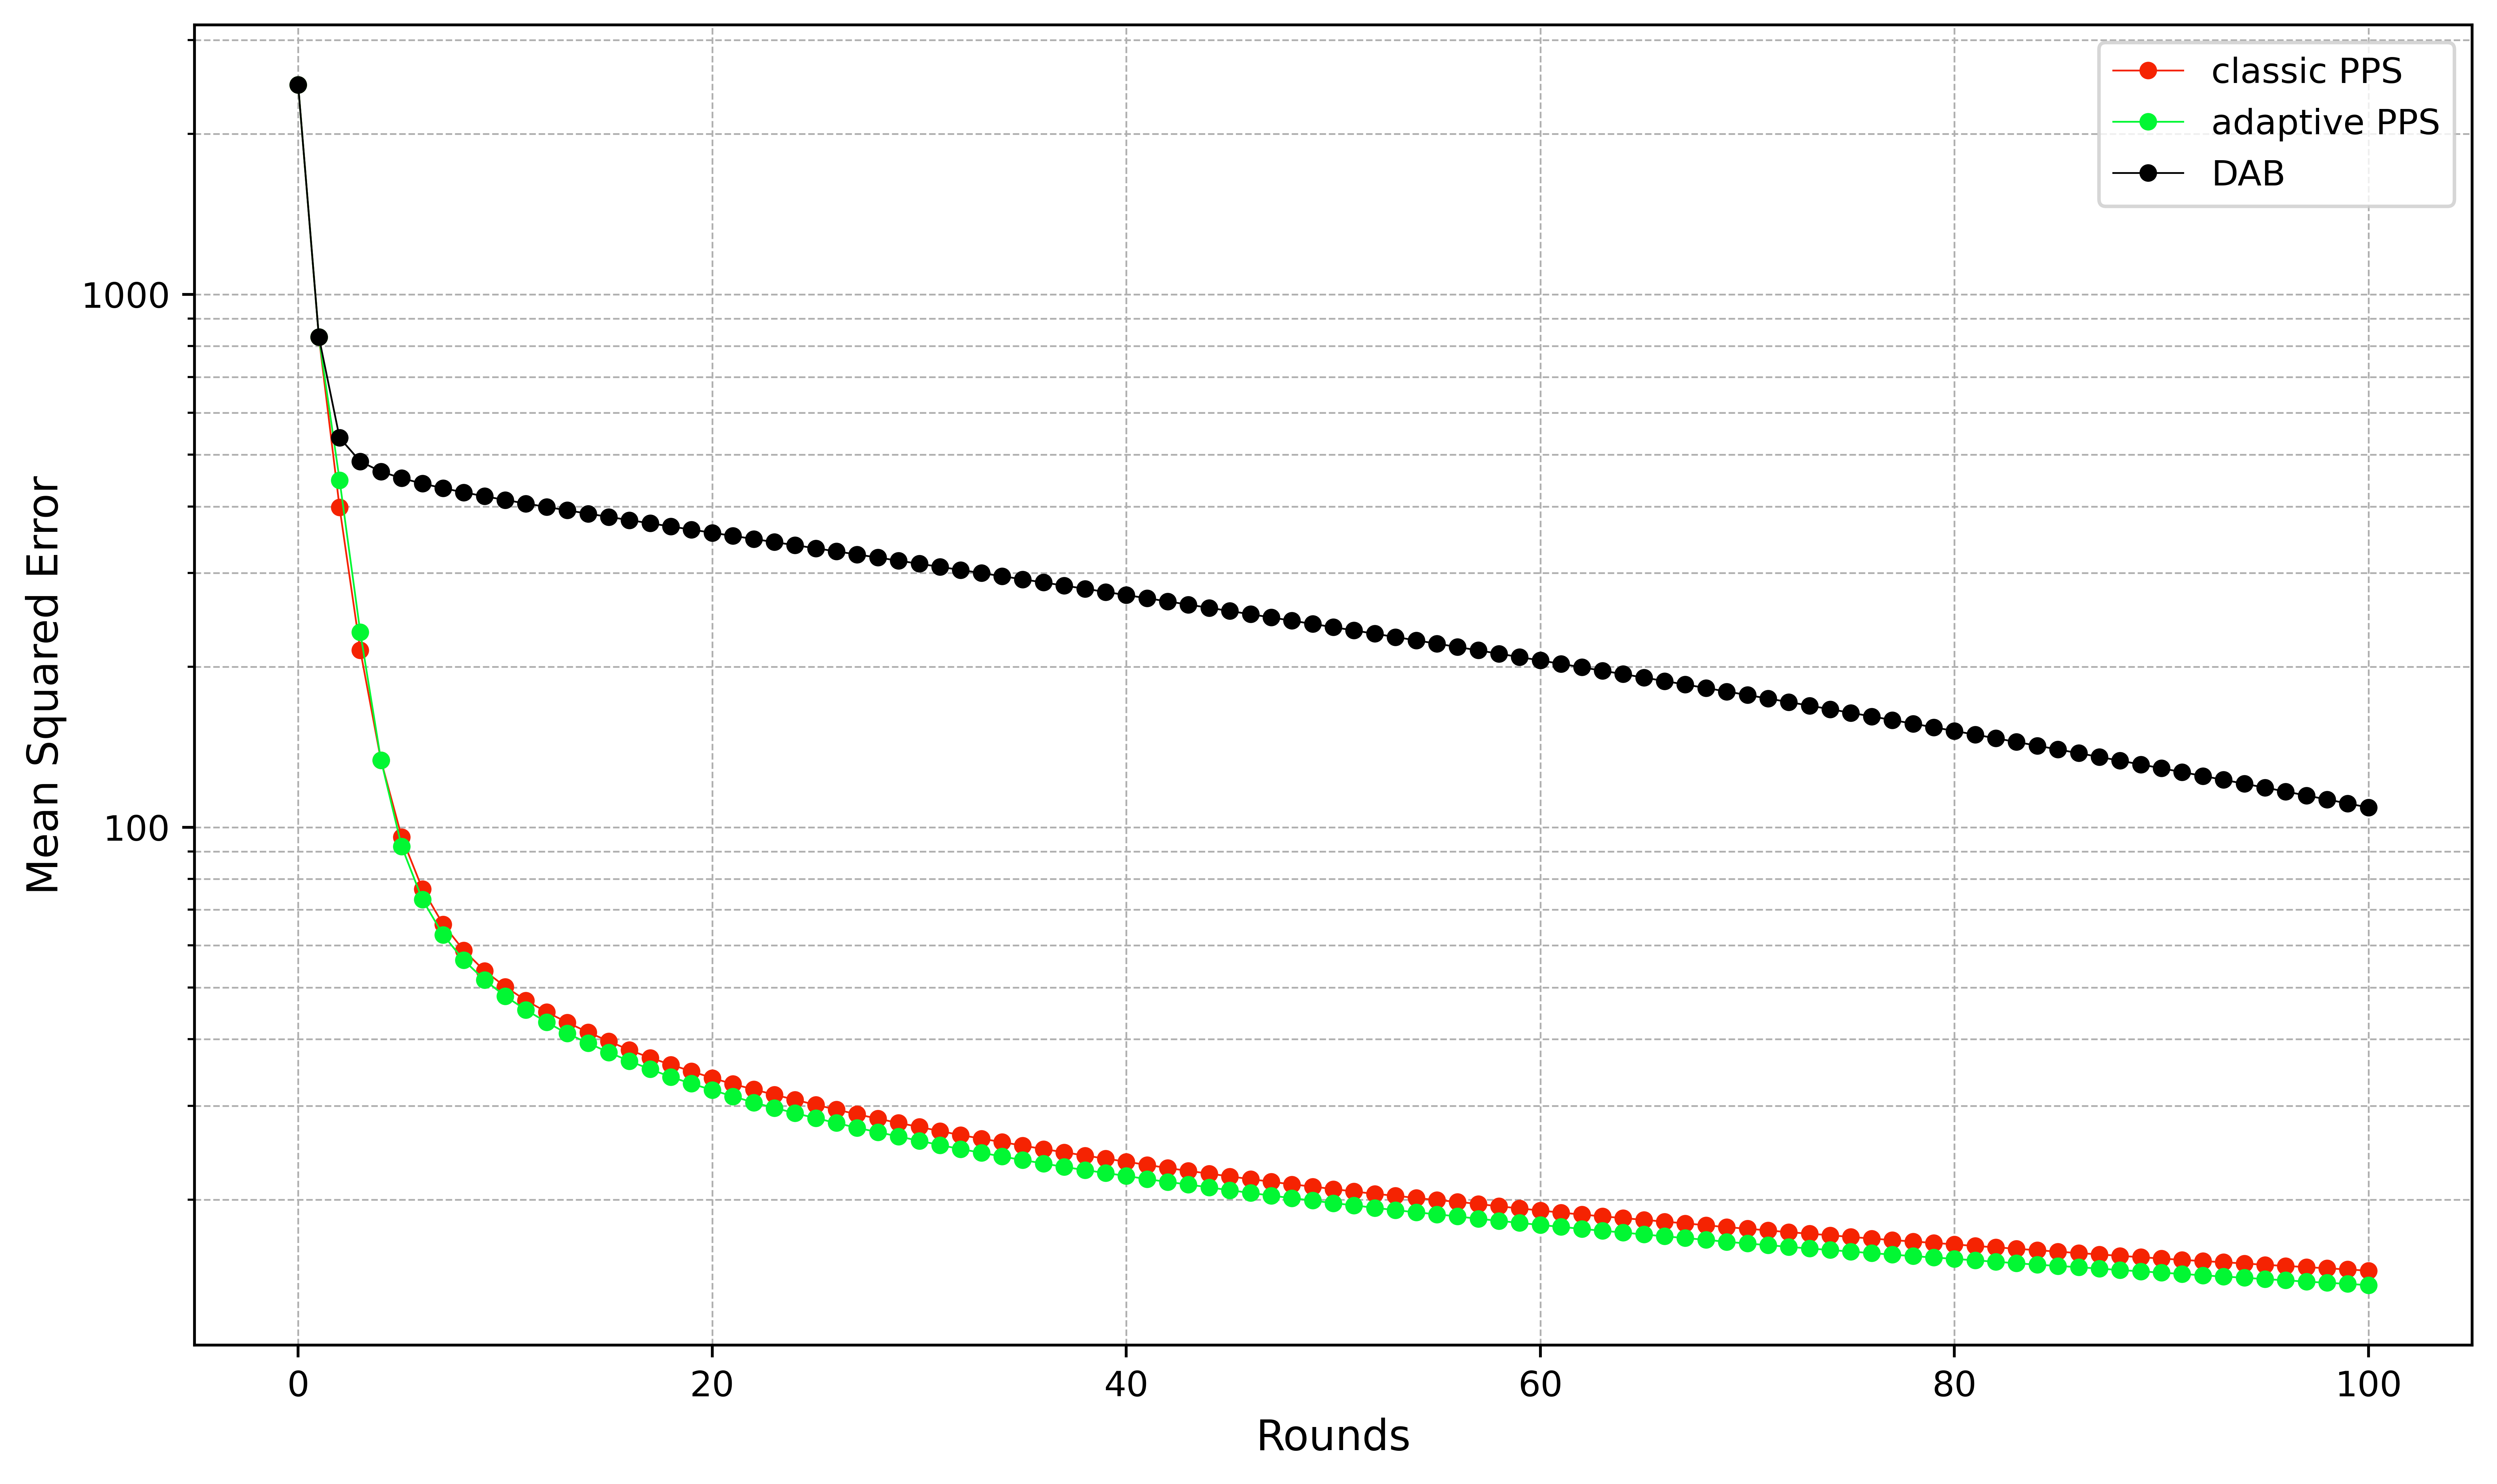
\includegraphics[width=\linewidth]{figures/Simulation_outcomes/LollipopGraph/512_512/DAB_vs_PPS_LG_r100_n1024_averaged_log.png}
    \caption{(512, 512)-Lollipop graph: mean squared error per rounds (log-linear)}
    \label{fig:lollipopgraphMSEperRoundLogLog}
\end{figure}

\begin{figure}[]
    \centering
    \scalebox{0.8}{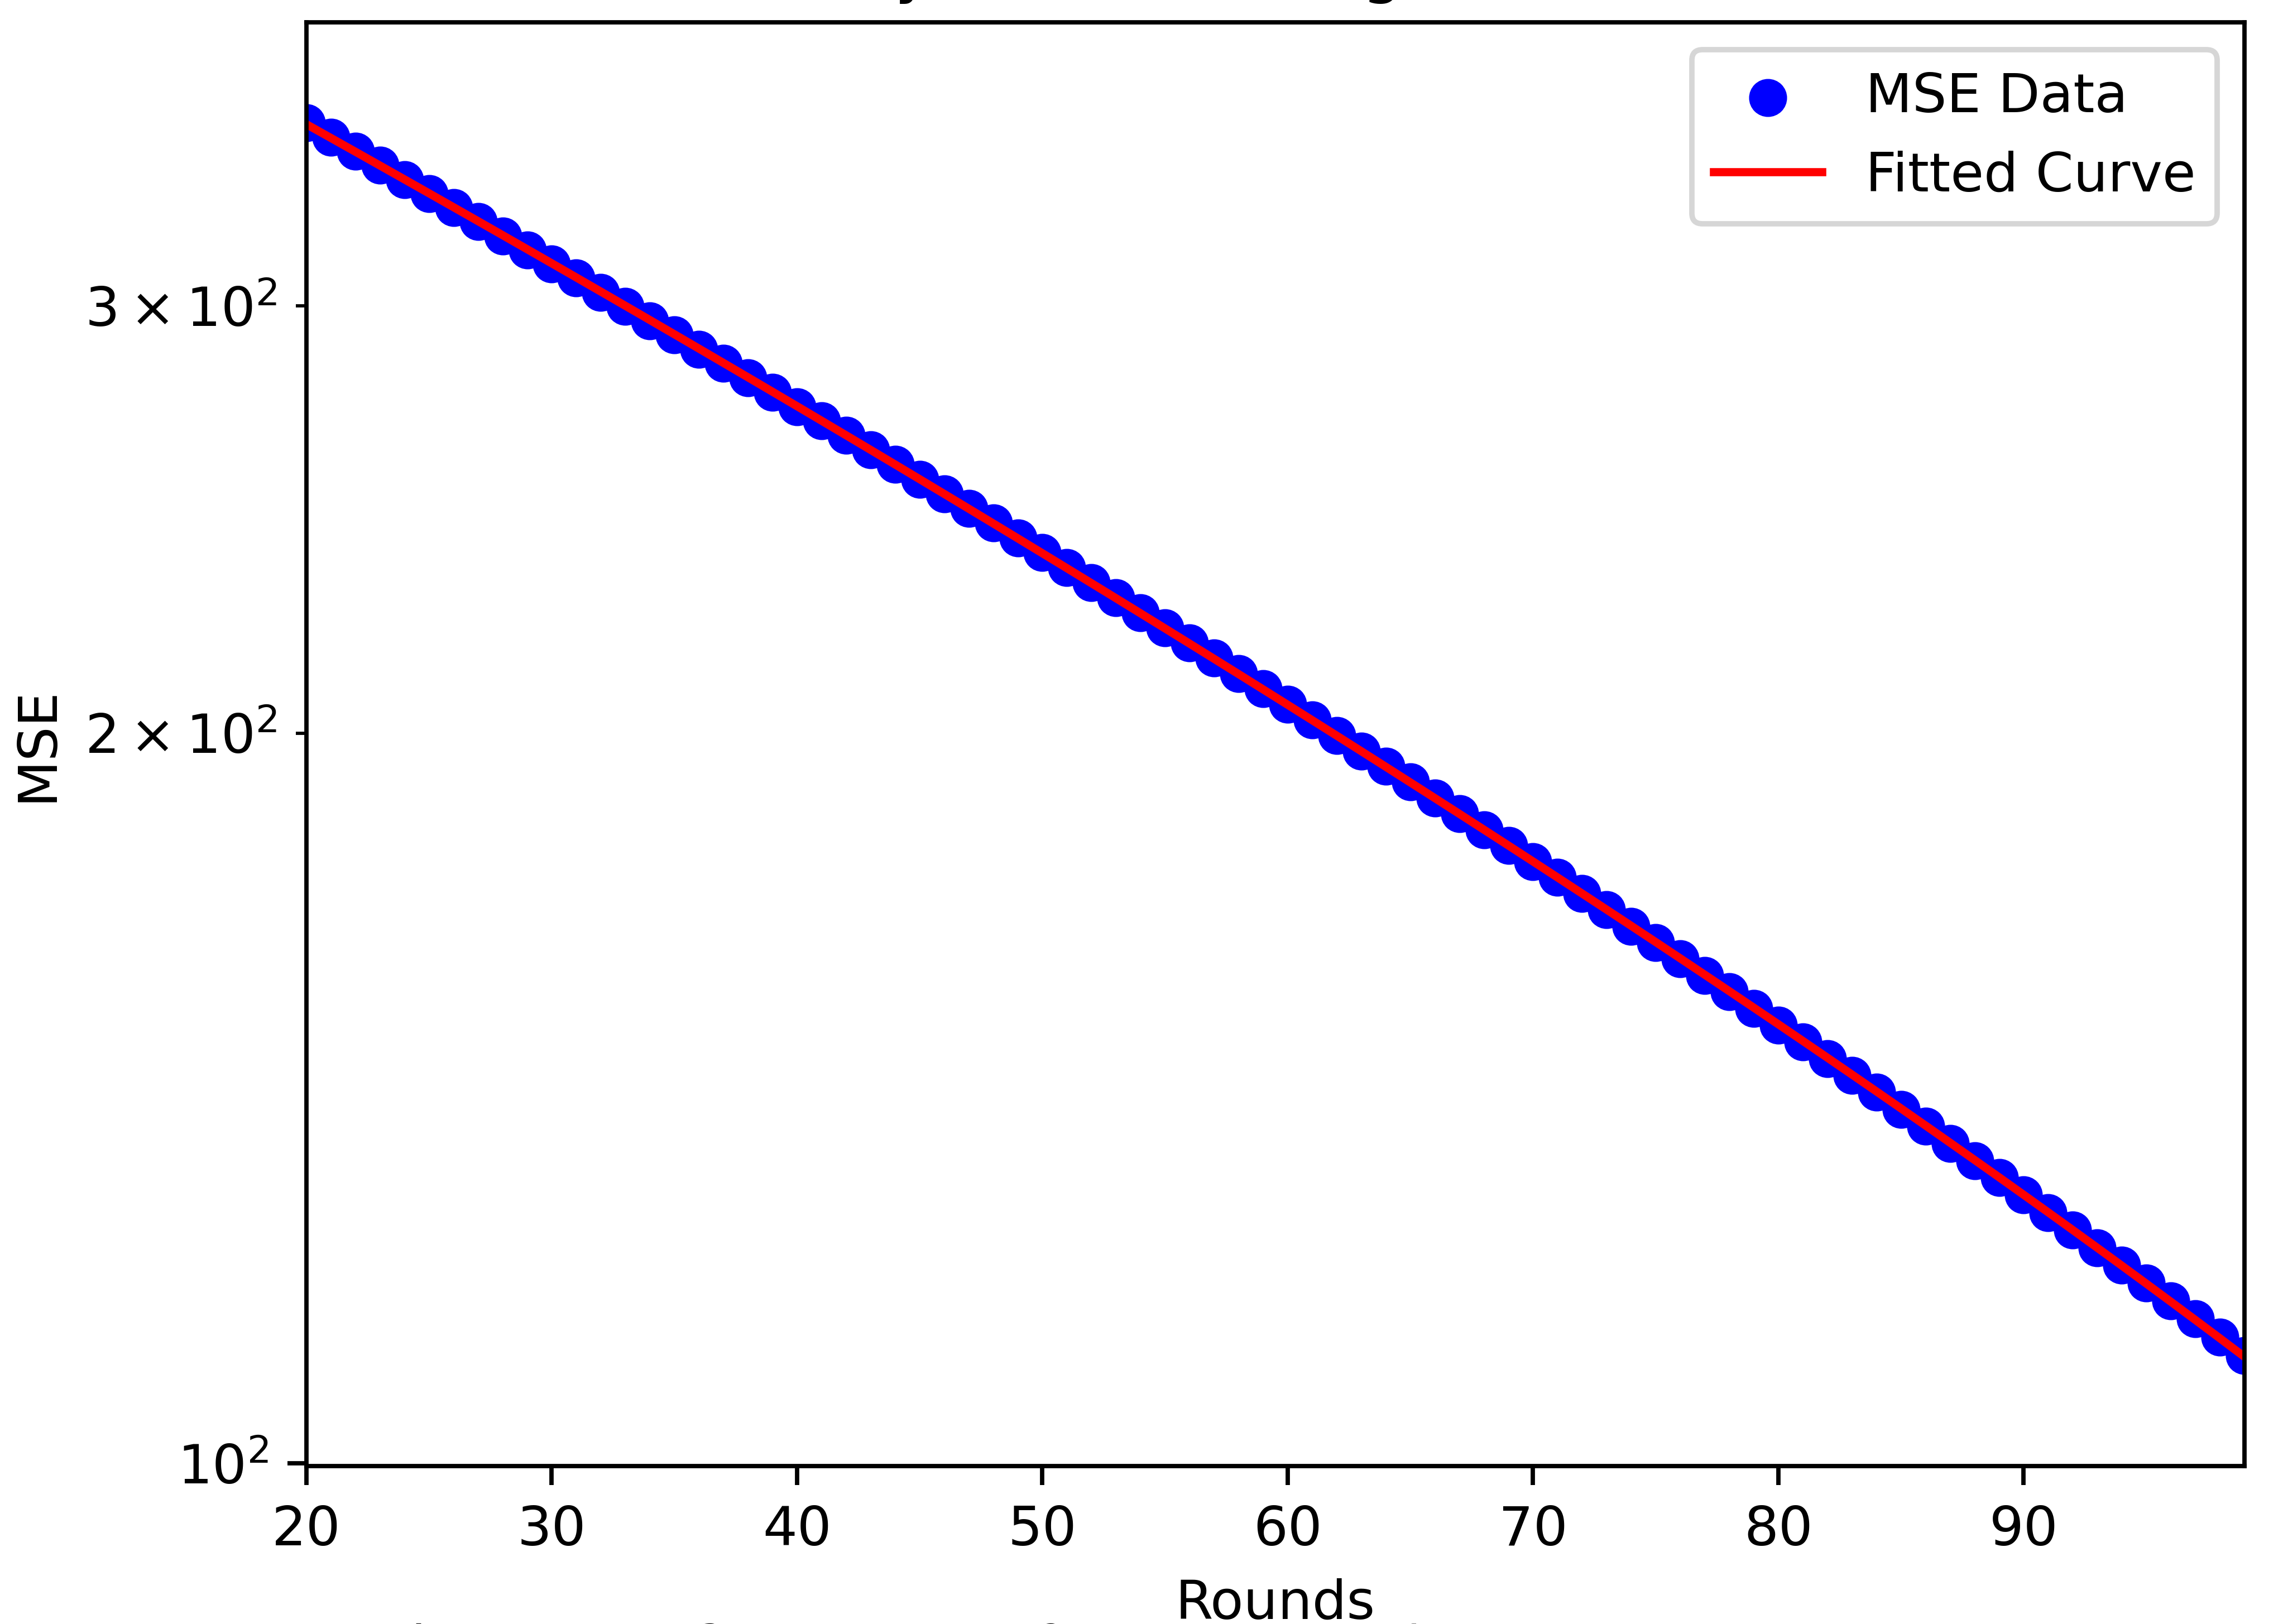
\includegraphics{figures/Simulation_outcomes/LollipopGraph/512_512/DAB/DAB_modelfitting_rounds_99_model_2.png}}
    \caption{(512, 512)-Lollipop graph - polynomial regression fit: DAB}
    \label{fig:dablollipopgraphModelFit}
\end{figure}

\begin{figure}[]
    \centering
    \scalebox{0.8}{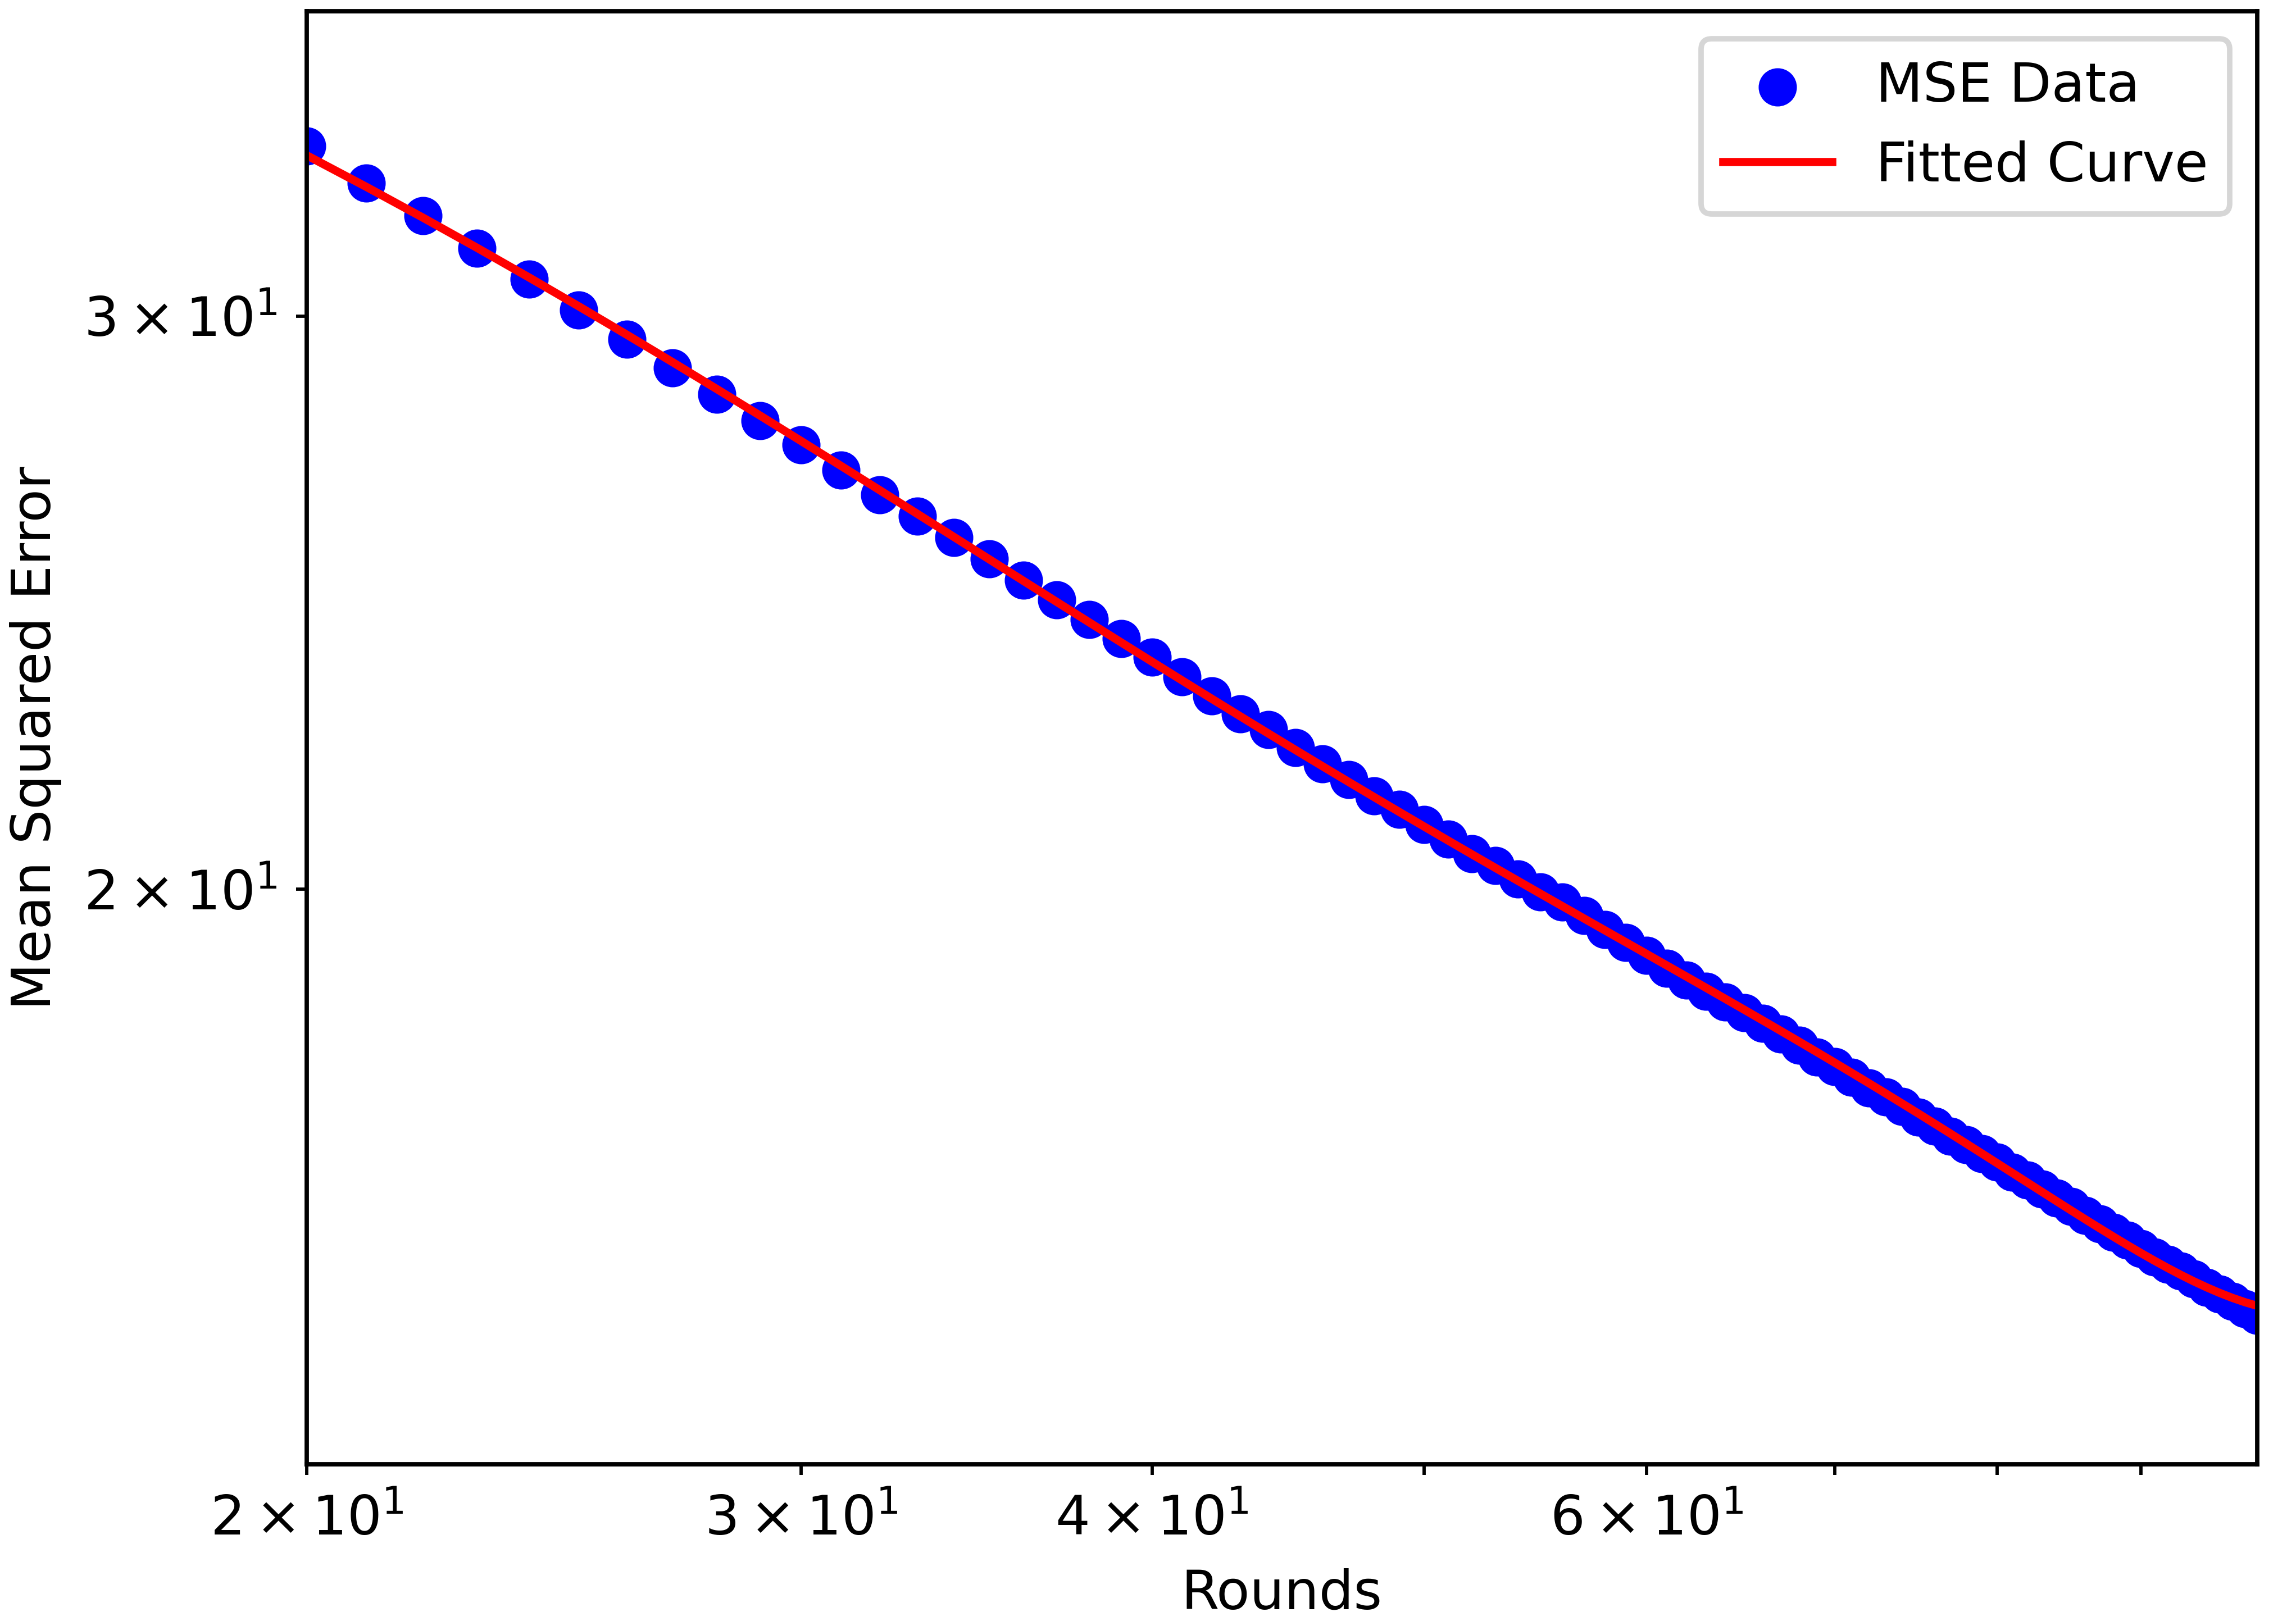
\includegraphics{figures/Simulation_outcomes/LollipopGraph/512_512/PPS/PPS_modelfitting_rounds_99_model_2.png}}
    \caption{(512, 512)-Lollipop graph - polynomial regression fit: PPS}
    \label{fig:ppslollipopgraphModelFit}
\end{figure}

\begin{figure}[]
    \centering
    \scalebox{0.8}{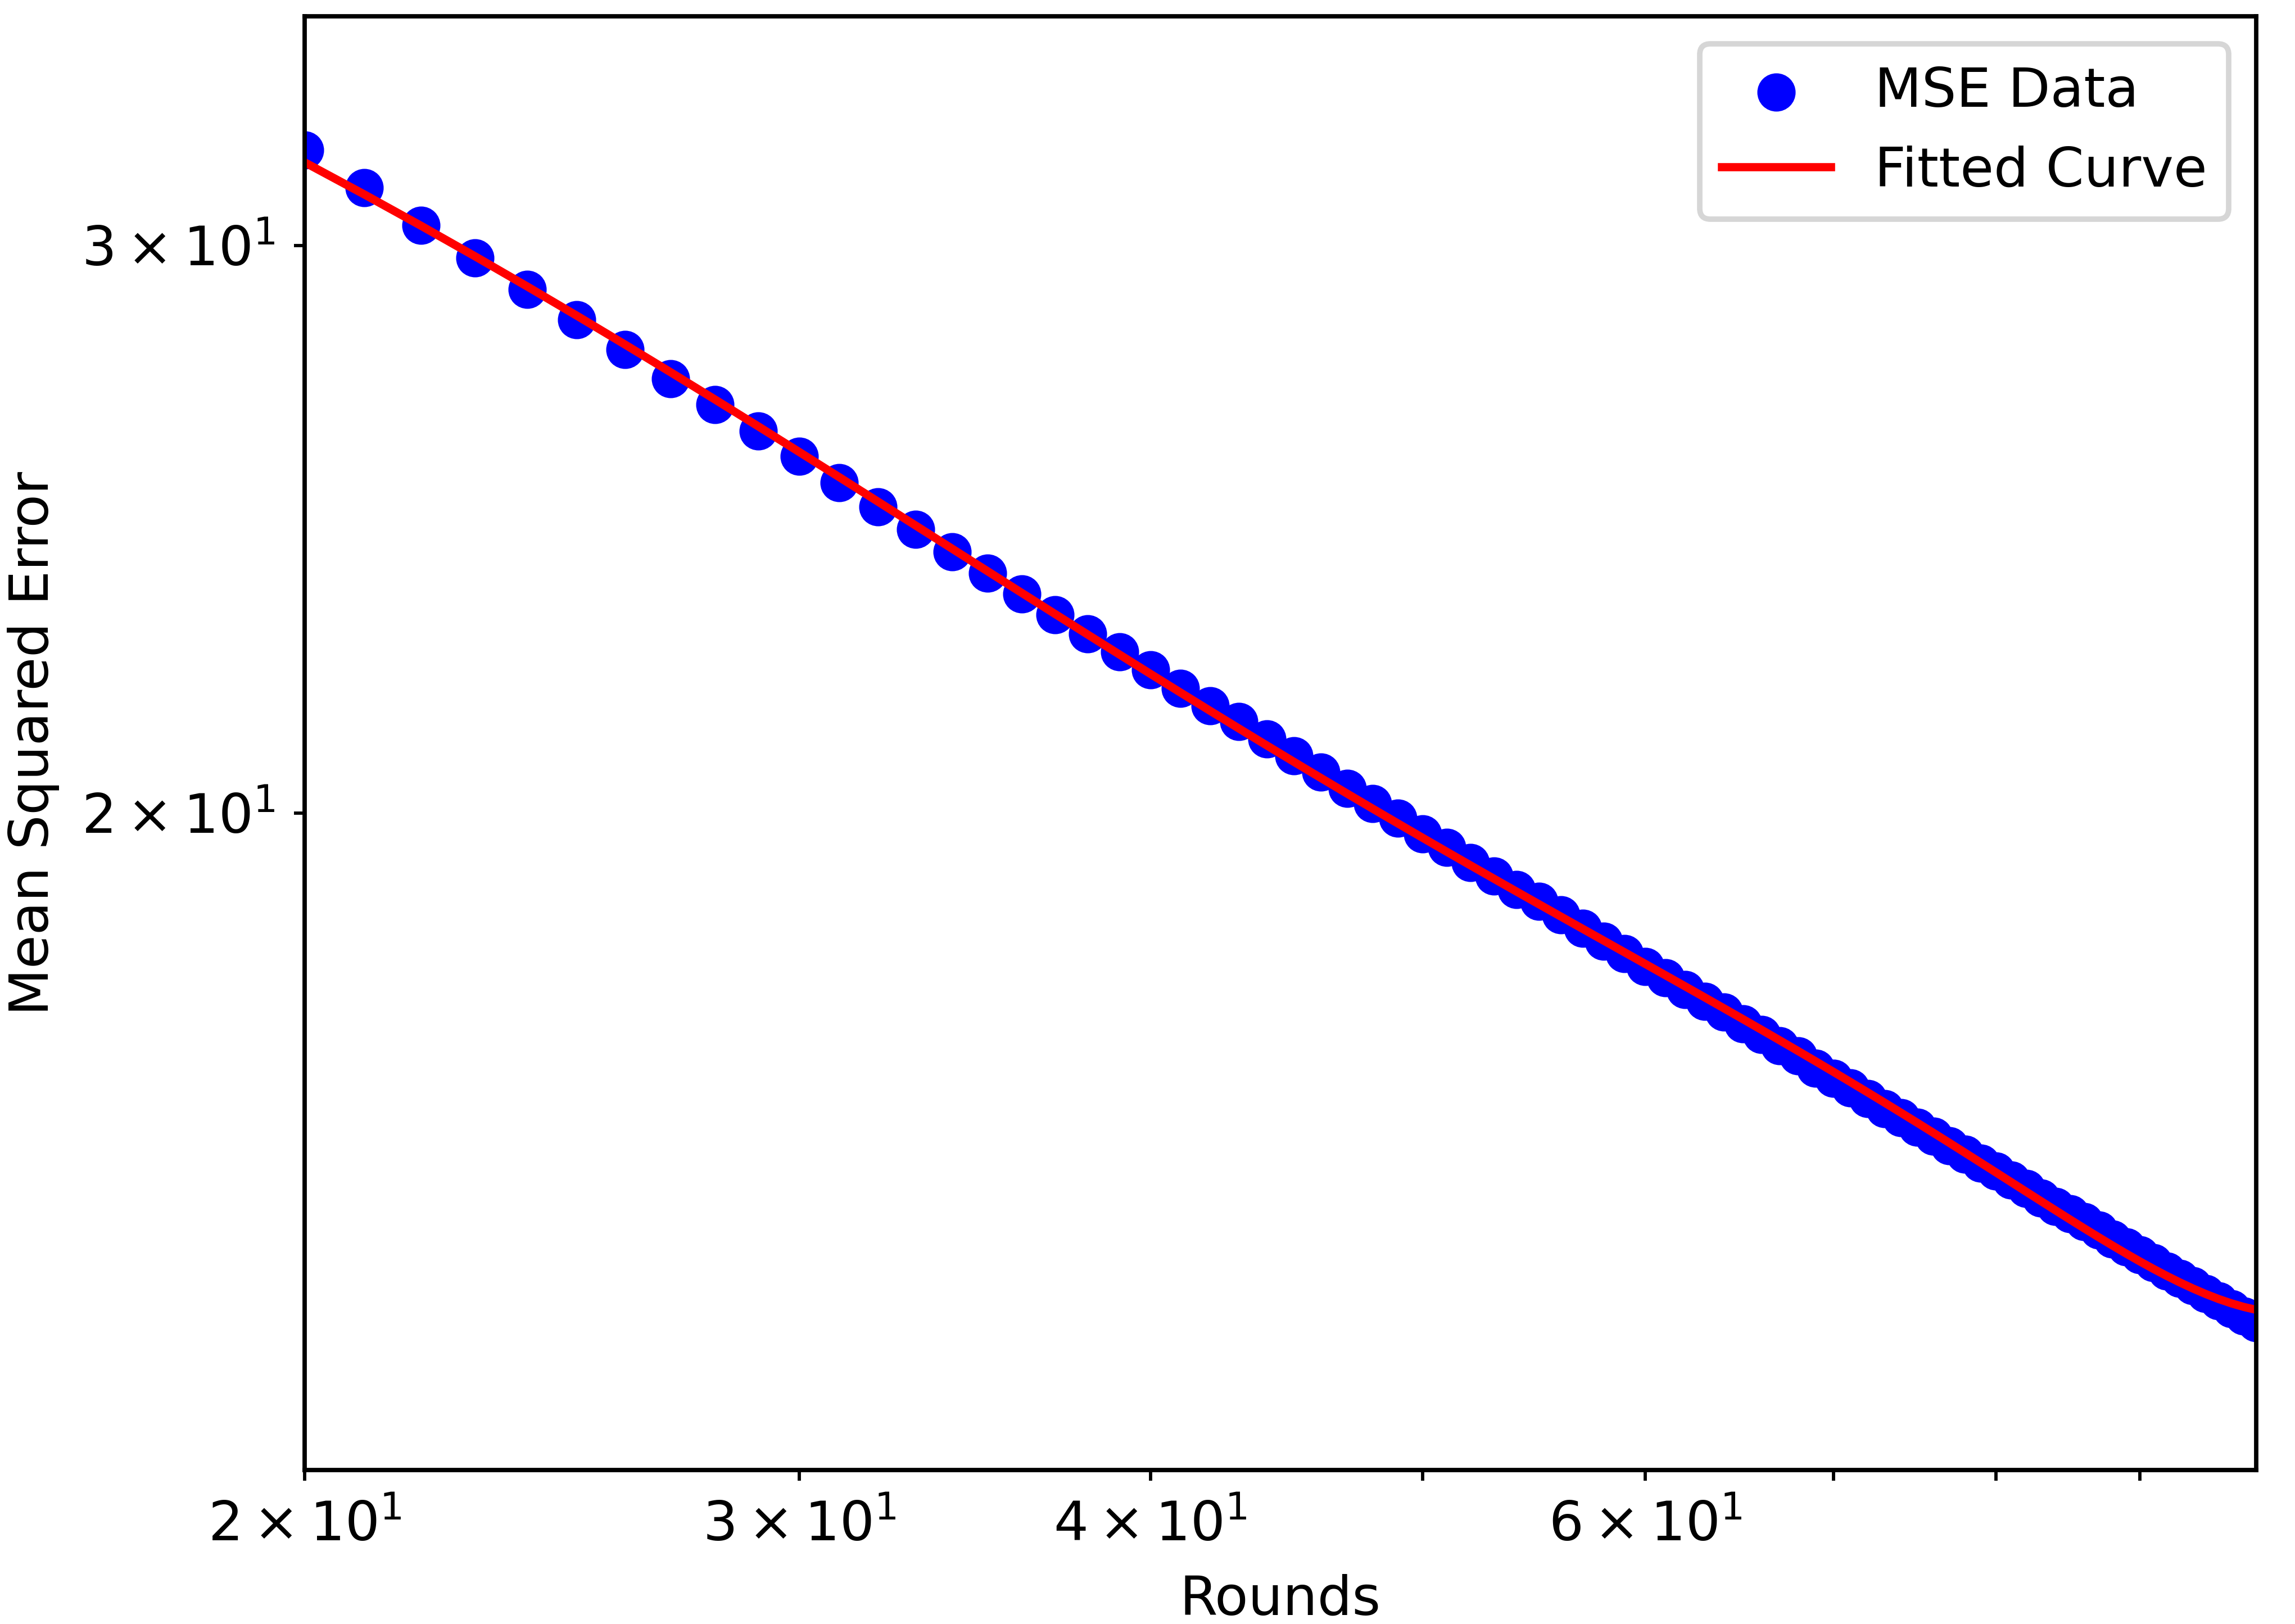
\includegraphics{figures/Simulation_outcomes/LollipopGraph/512_512/ATPPS/ATPPS_modelfitting_rounds_99_model_2.png}}
    \caption{(512, 512)-Lollipop graph - polynomial regression fit: ATPPS}
    \label{fig:atppslollipopgraphModelFit}
\end{figure}

\begin{figure}
    \centering
    \scalebox{0.8}{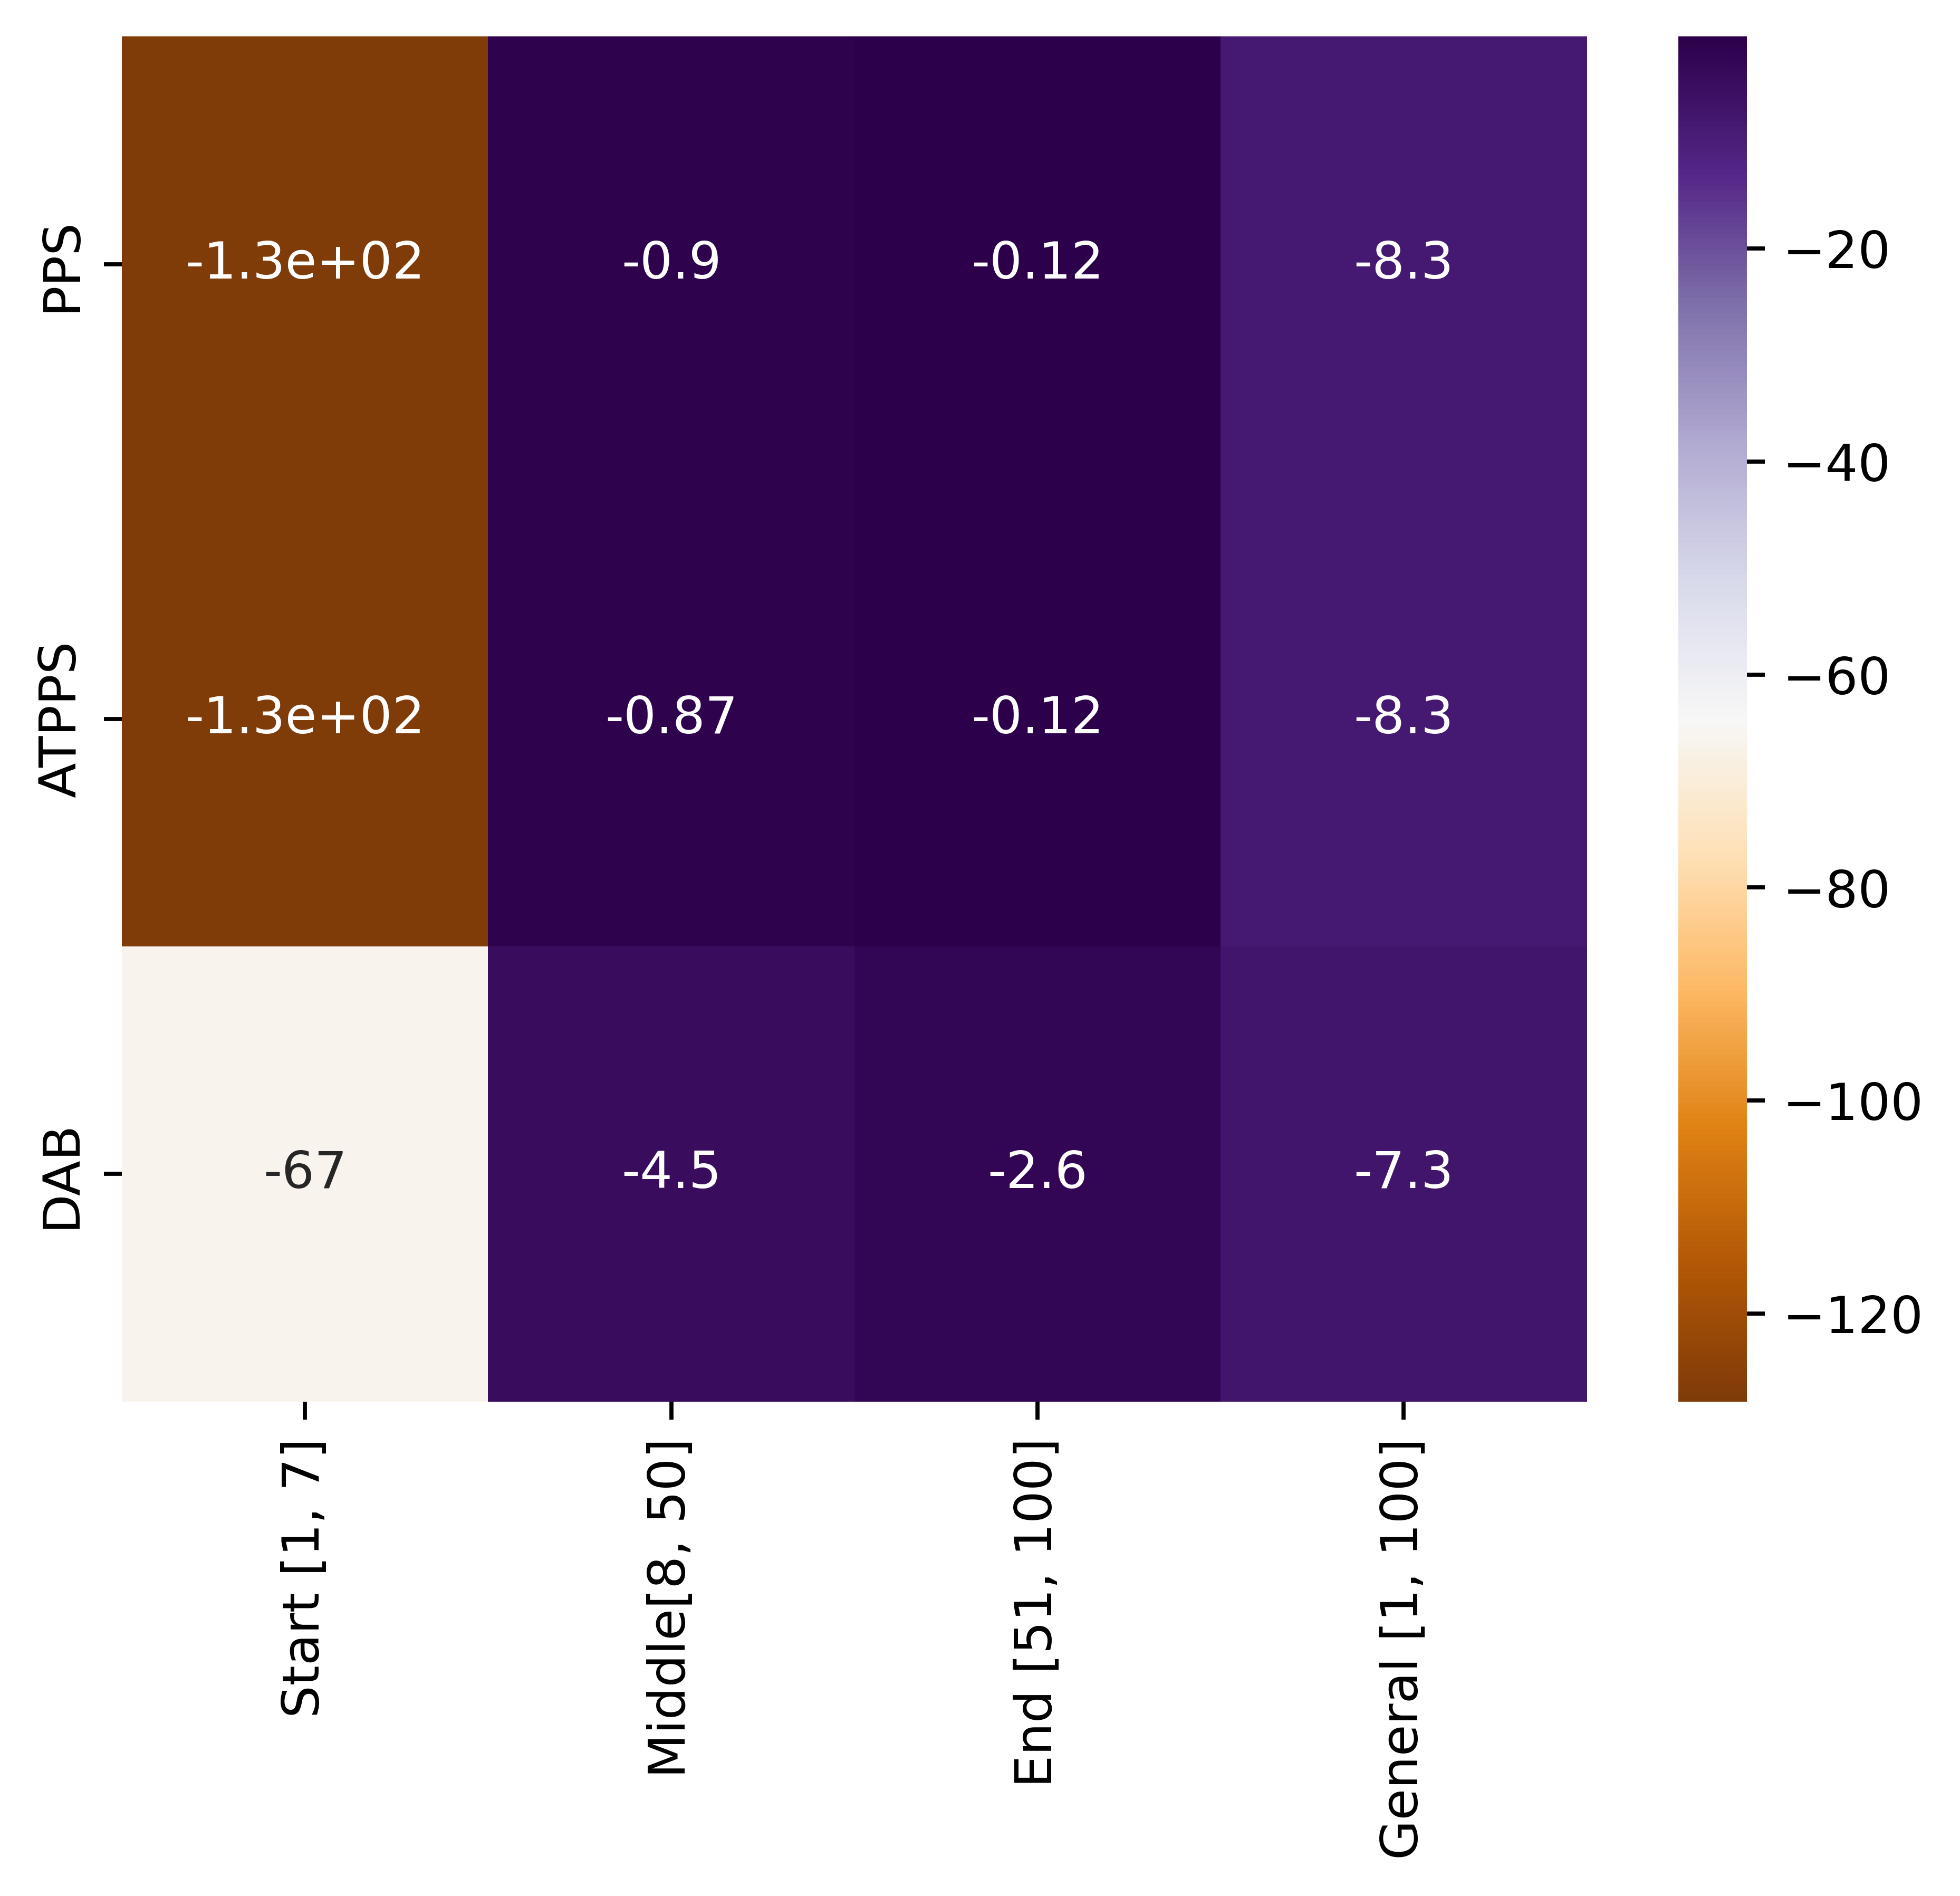
\includegraphics{figures/Simulation_outcomes/LollipopGraph/512_512/DAB_vs_PPS_vs_ATPPS_slopesheatmap_100rounds.png}}
    \caption{Lollipop graph: heat map of slopes per region}
    \label{fig:lollipopslopes}
\end{figure}

To analyze the impact of the path size and clique size on the simulation results, additional simulations were conducted with varying proportions of nodes assigned to each region. In subsection \ref{subsec:128_896lollipop}, the number of nodes assigned to the clique is reduced to 128, which is one-fourth of the previous value of 512. Consequently, the path section now consists of 896 nodes. The total network size remains unchanged. This adjustment allows us to observe how a more dominant path section influences the load balancing behavior of the different algorithms. Similarly, in subsection \ref{subsec:896_128lollipop}, the simulations are performed with a reduced path size, assigning 896 nodes to the clique and only 128 nodes to the path. This configuration provides insight into how a more densely connected clique affects the overall performance of the algorithms.

\subsection{(128, 896) Lollipop Graph}\label{subsec:128_896lollipop}
In the initial phase (the first 7 rounds) PPS and ATPPS start with a steep decline in MSE, both with a slope of -86, as shown in figure \ref{fig:128_896lollipopslopes}. DAB, on the other hand, demonstrates a slightly slower initial convergence, with a slope of -110. Compared to the previous experiment, where the path and clique sizes were equal, DAB's performance in the initial rounds has improved. The slope in this region in the previous experiment was -68 and improved to -110, which indicates a faster initial error reduction. In the middle region, rounds 8 to 50, the ATPPS shows a performance close to that of the PPS where both curves maintain a consistently steep slope. In this phase, DAB exhibits the steepest slope, reducing the error by an average of -2.8 per round. Meanwhile, PPS and ATPPS, having already achieved low MSE values due to their rapid initial reduction, decrease the error by approximately -1.5 per round on average. In the end phase the DAB shows a slightly sharper decline in MSE compared to earlier rounds. This could be attributed to the longer path structure of the graph: once most of the load has propagated through the clique, the balancing process along the path accelerates. Despite this, both Push-Pull Sum variants continue to outperform DAB, achieving lower MSE values in fewer rounds due to their efficient clique-based load redistribution. Interestingly, PPS and ATPPS exhibit a slight divergence between rounds 10 and 90, before finally intersecting (or nearly so) around round 100.

\begin{figure}[]
    \centering
    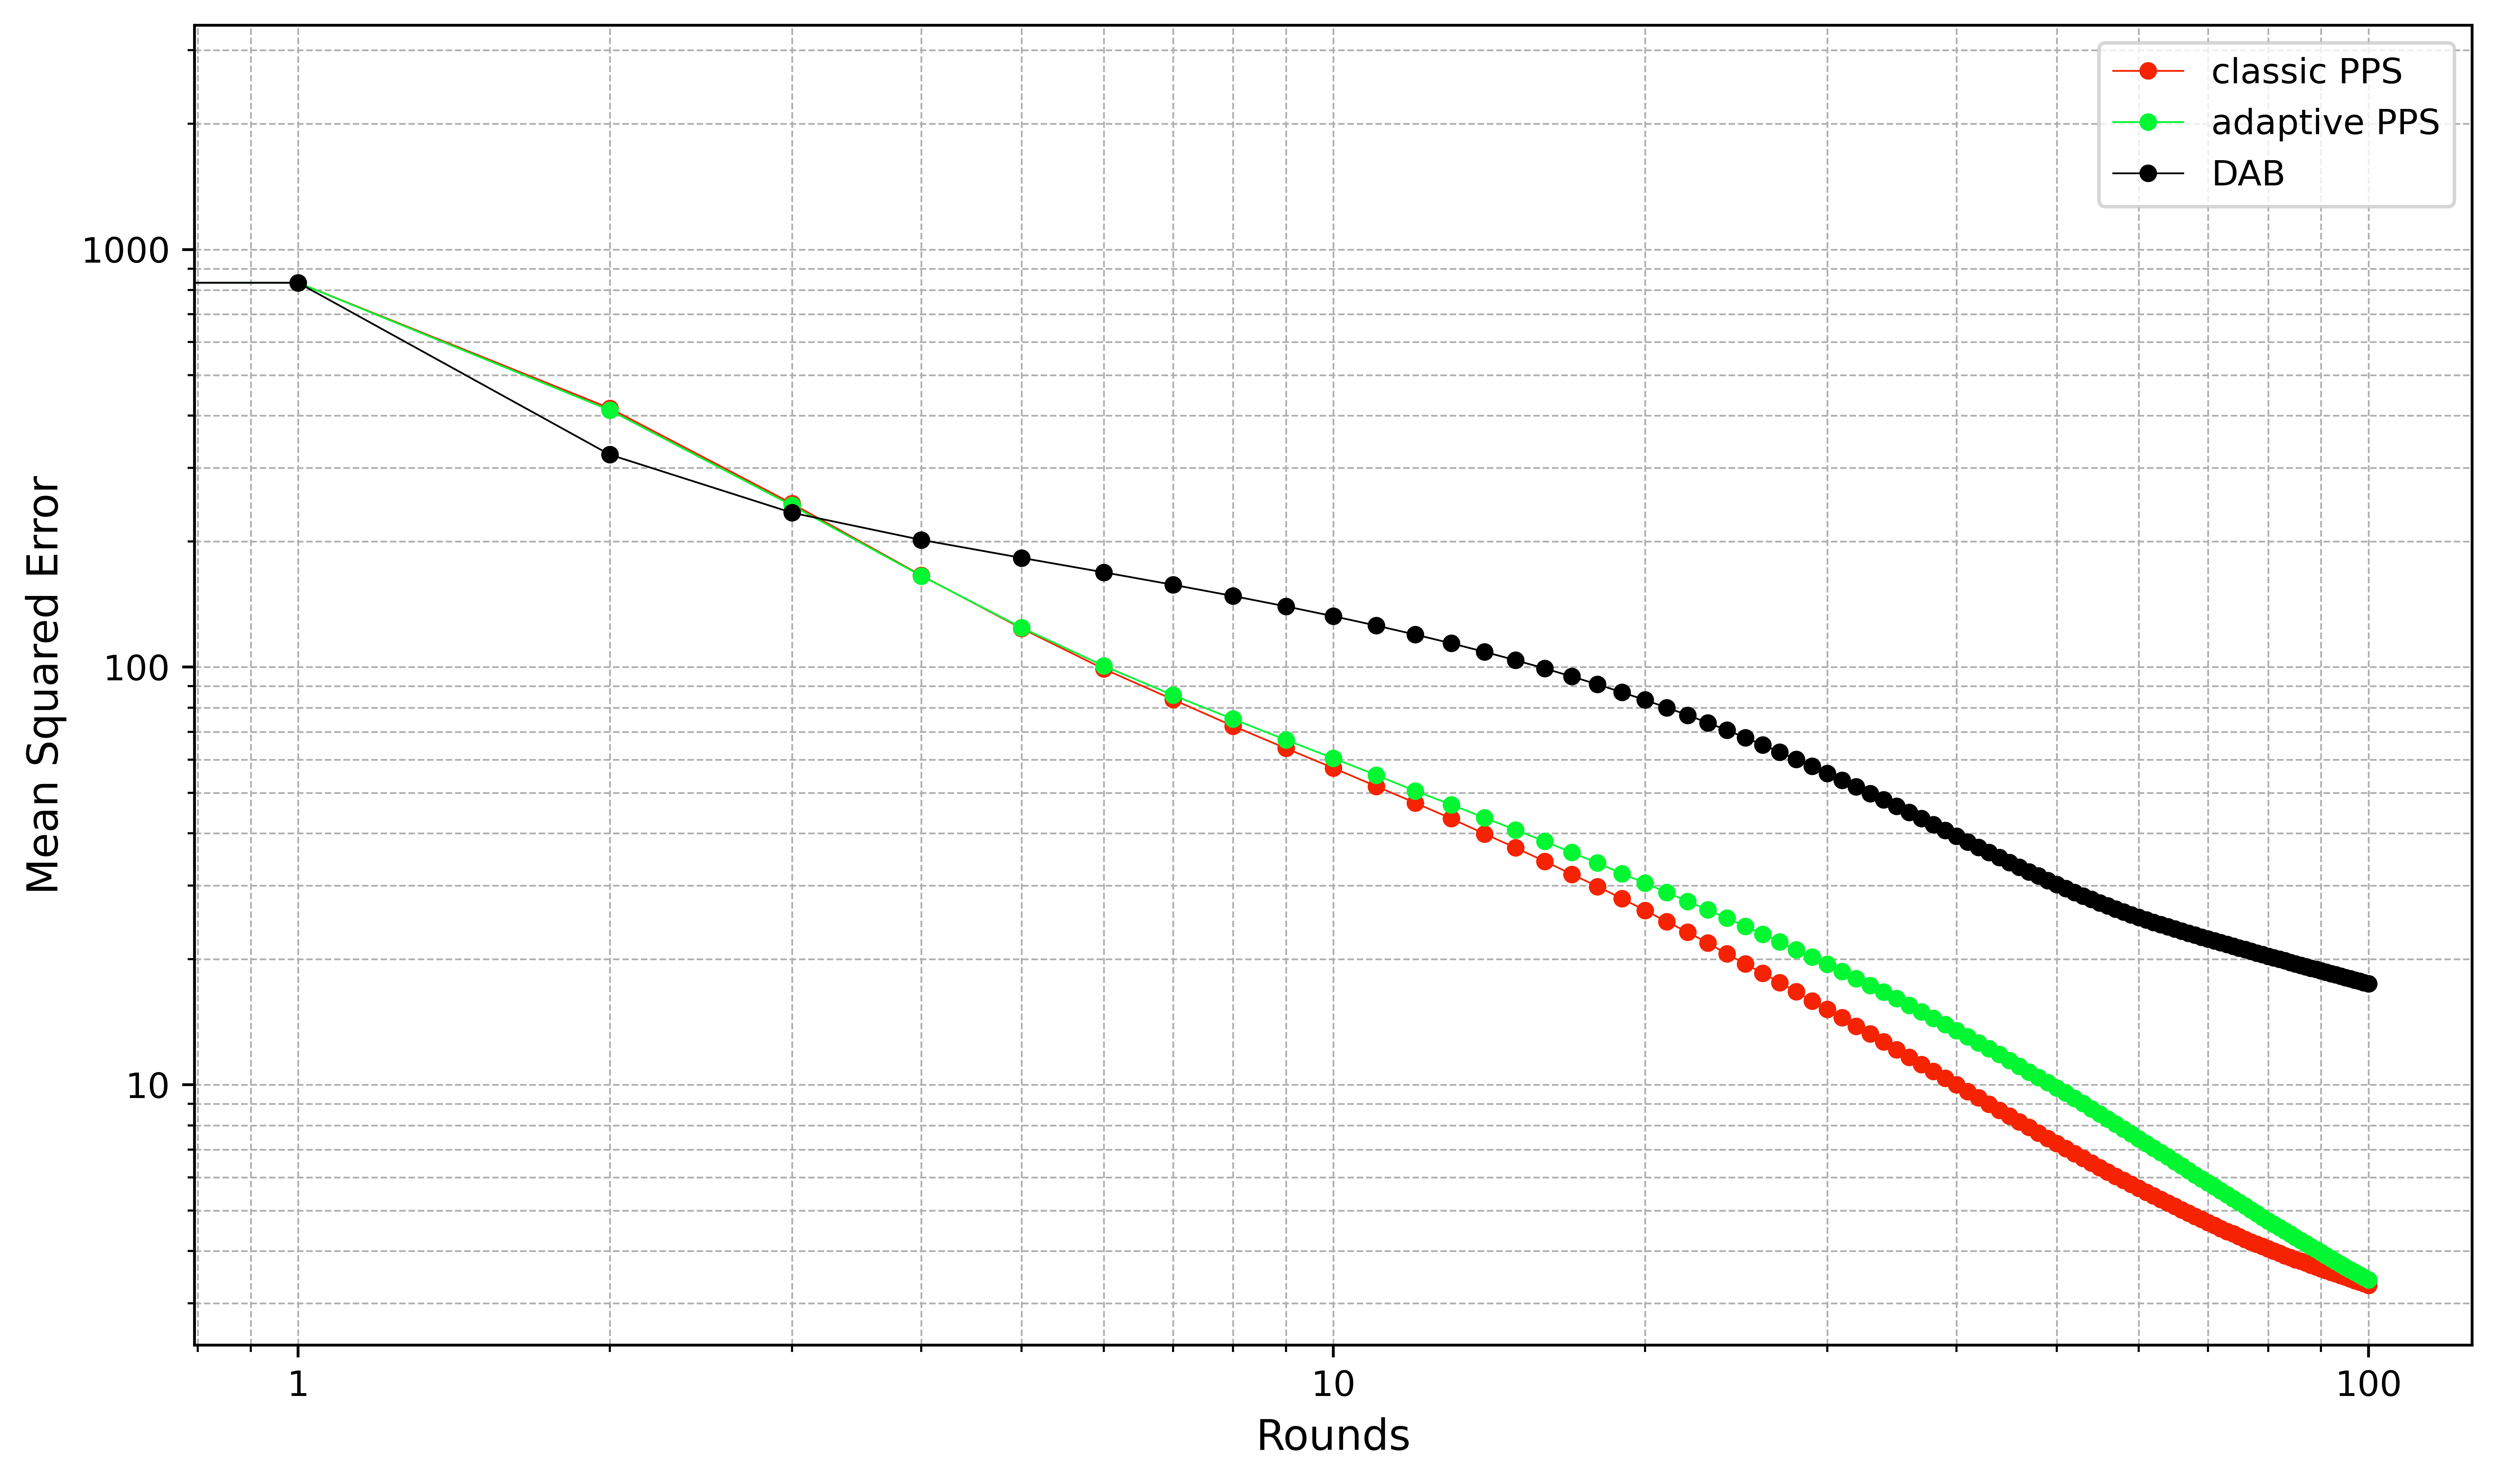
\includegraphics[width=\linewidth]{figures/Simulation_outcomes/LollipopGraph/128_896/DAB_vs_PPS_LG_r100_n1024_averaged_loglog.png}
    \caption{(128, 896)-Lollipop graph: mean squared error per rounds (log-log)}
    \label{fig:128_896lollipopgraphMSEperRoundLogLog}
\end{figure}

The MSE data of all three load balancing algorithms were fitted to polynomial polynomial regression models. The MSE data for DAB and ATPPS were best approximated by polynomials of degree 4, while the PPS MSE data exhibited slightly more complex behavior, following a polynomial of degree 5. The fitted model for the DAB MSE data follows the equation: $MSE_r=3.46\times 10^{-6}r^{4}-1.12\times 10^{-3}r^{3}+0.14r^{2}-7.69r+190.78$ (figure \ref{fig:dab_128x896lollipopgraphModelFit}). For ATPPS, the polynomial fit is given by $MSE_r=1.59\times 10^{-6}r^{4}-4.74\times 10^{-4}r^{3}+0.054r^{2}-2.94r+70.59$ (figure \ref{fig:pps_128x896lollipopgraphModelFit}). The PPS MSE data, which required a higher-degree polynomial (degree 5), follows the equation $MSE_r=-3.72\times 10^{-8}r^{5}+1.31\times 10^{-5}r^{4}-1.85\times 10^{-3}r^{3}+0.13r^{2}-4.96r+84.91$ (figure \ref{fig:atpps_128x896lollipopgraphModelFit}).

\begin{figure}[]
    \centering
    \scalebox{0.8}{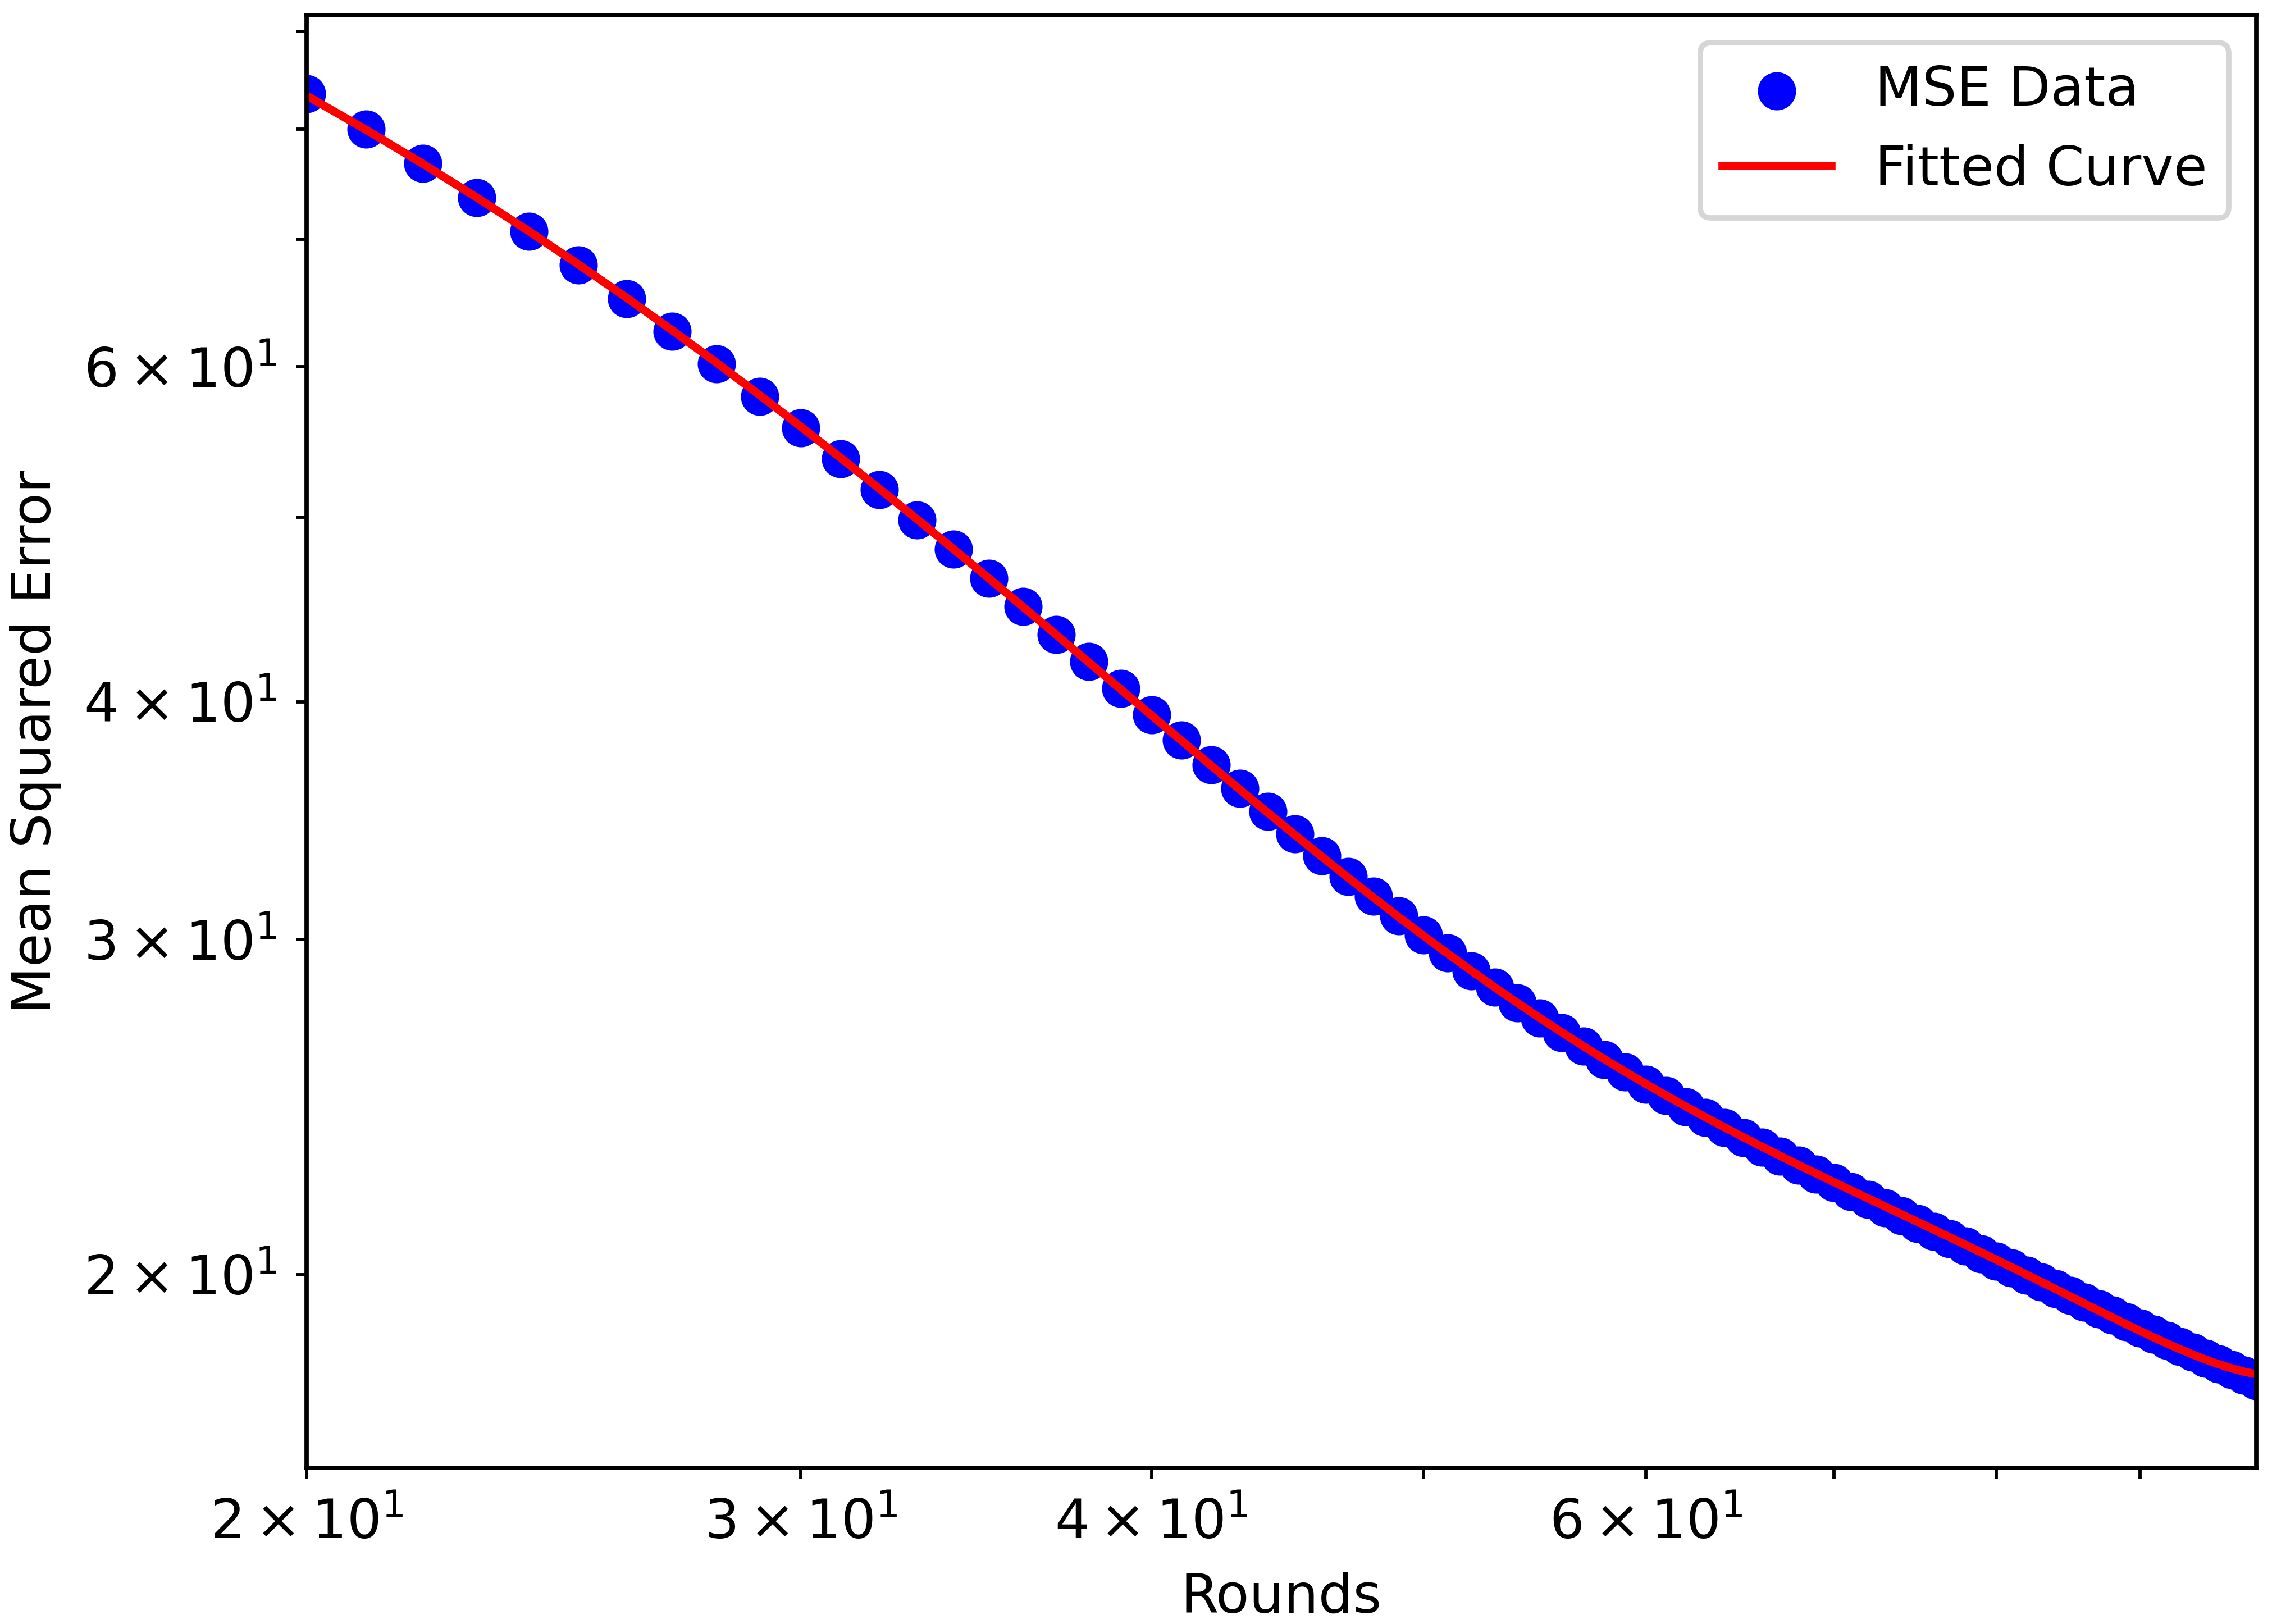
\includegraphics{figures/Simulation_outcomes/LollipopGraph/128_896/DAB/DAB_modelfitting_rounds_99_model_2.png}}
    \caption{(128, 896)-Lollipop graph - polynomial regression fit: DAB}
    \label{fig:dab_128x896lollipopgraphModelFit}
\end{figure}

\begin{figure}[]
    \centering
    \scalebox{0.8}{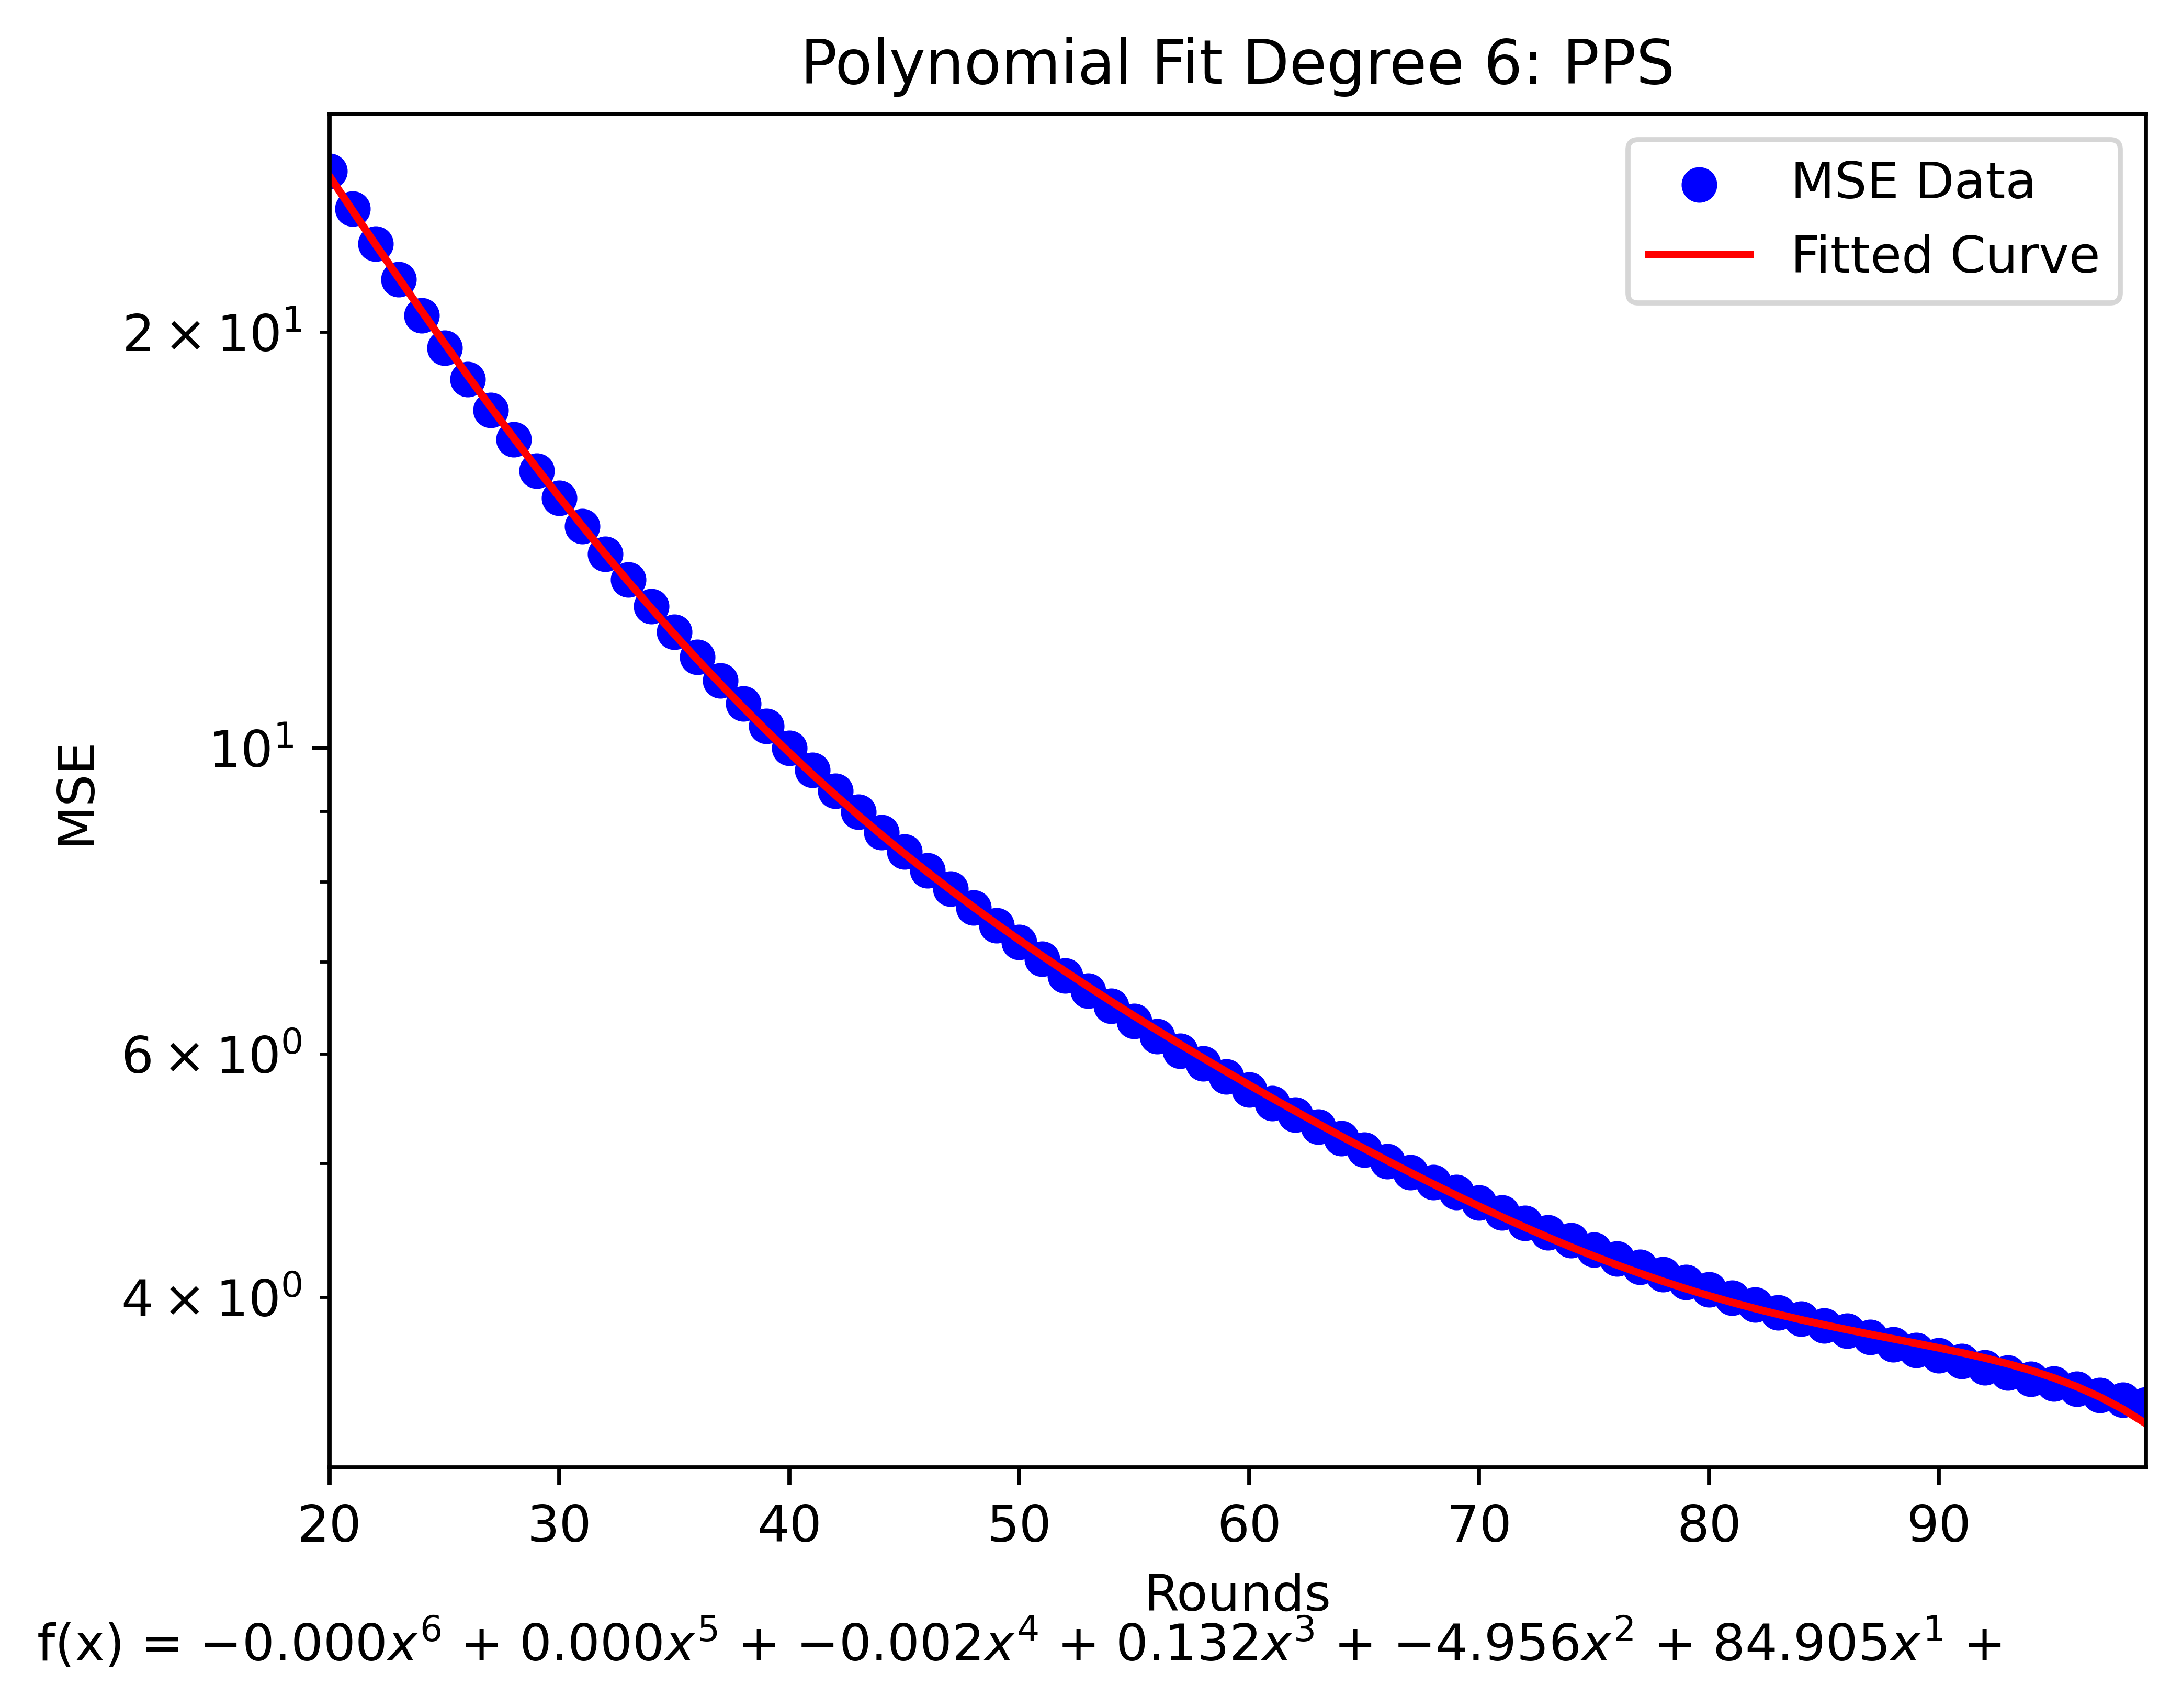
\includegraphics{figures/Simulation_outcomes/LollipopGraph/128_896/PPS/PPS_modelfitting_rounds_99_model_2.png}}
    \caption{(128, 896)-Lollipop graph - polynomial regression fit: PPS}
    \label{fig:pps_128x896lollipopgraphModelFit}
\end{figure}

\begin{figure}[]
    \centering
    \scalebox{0.8}{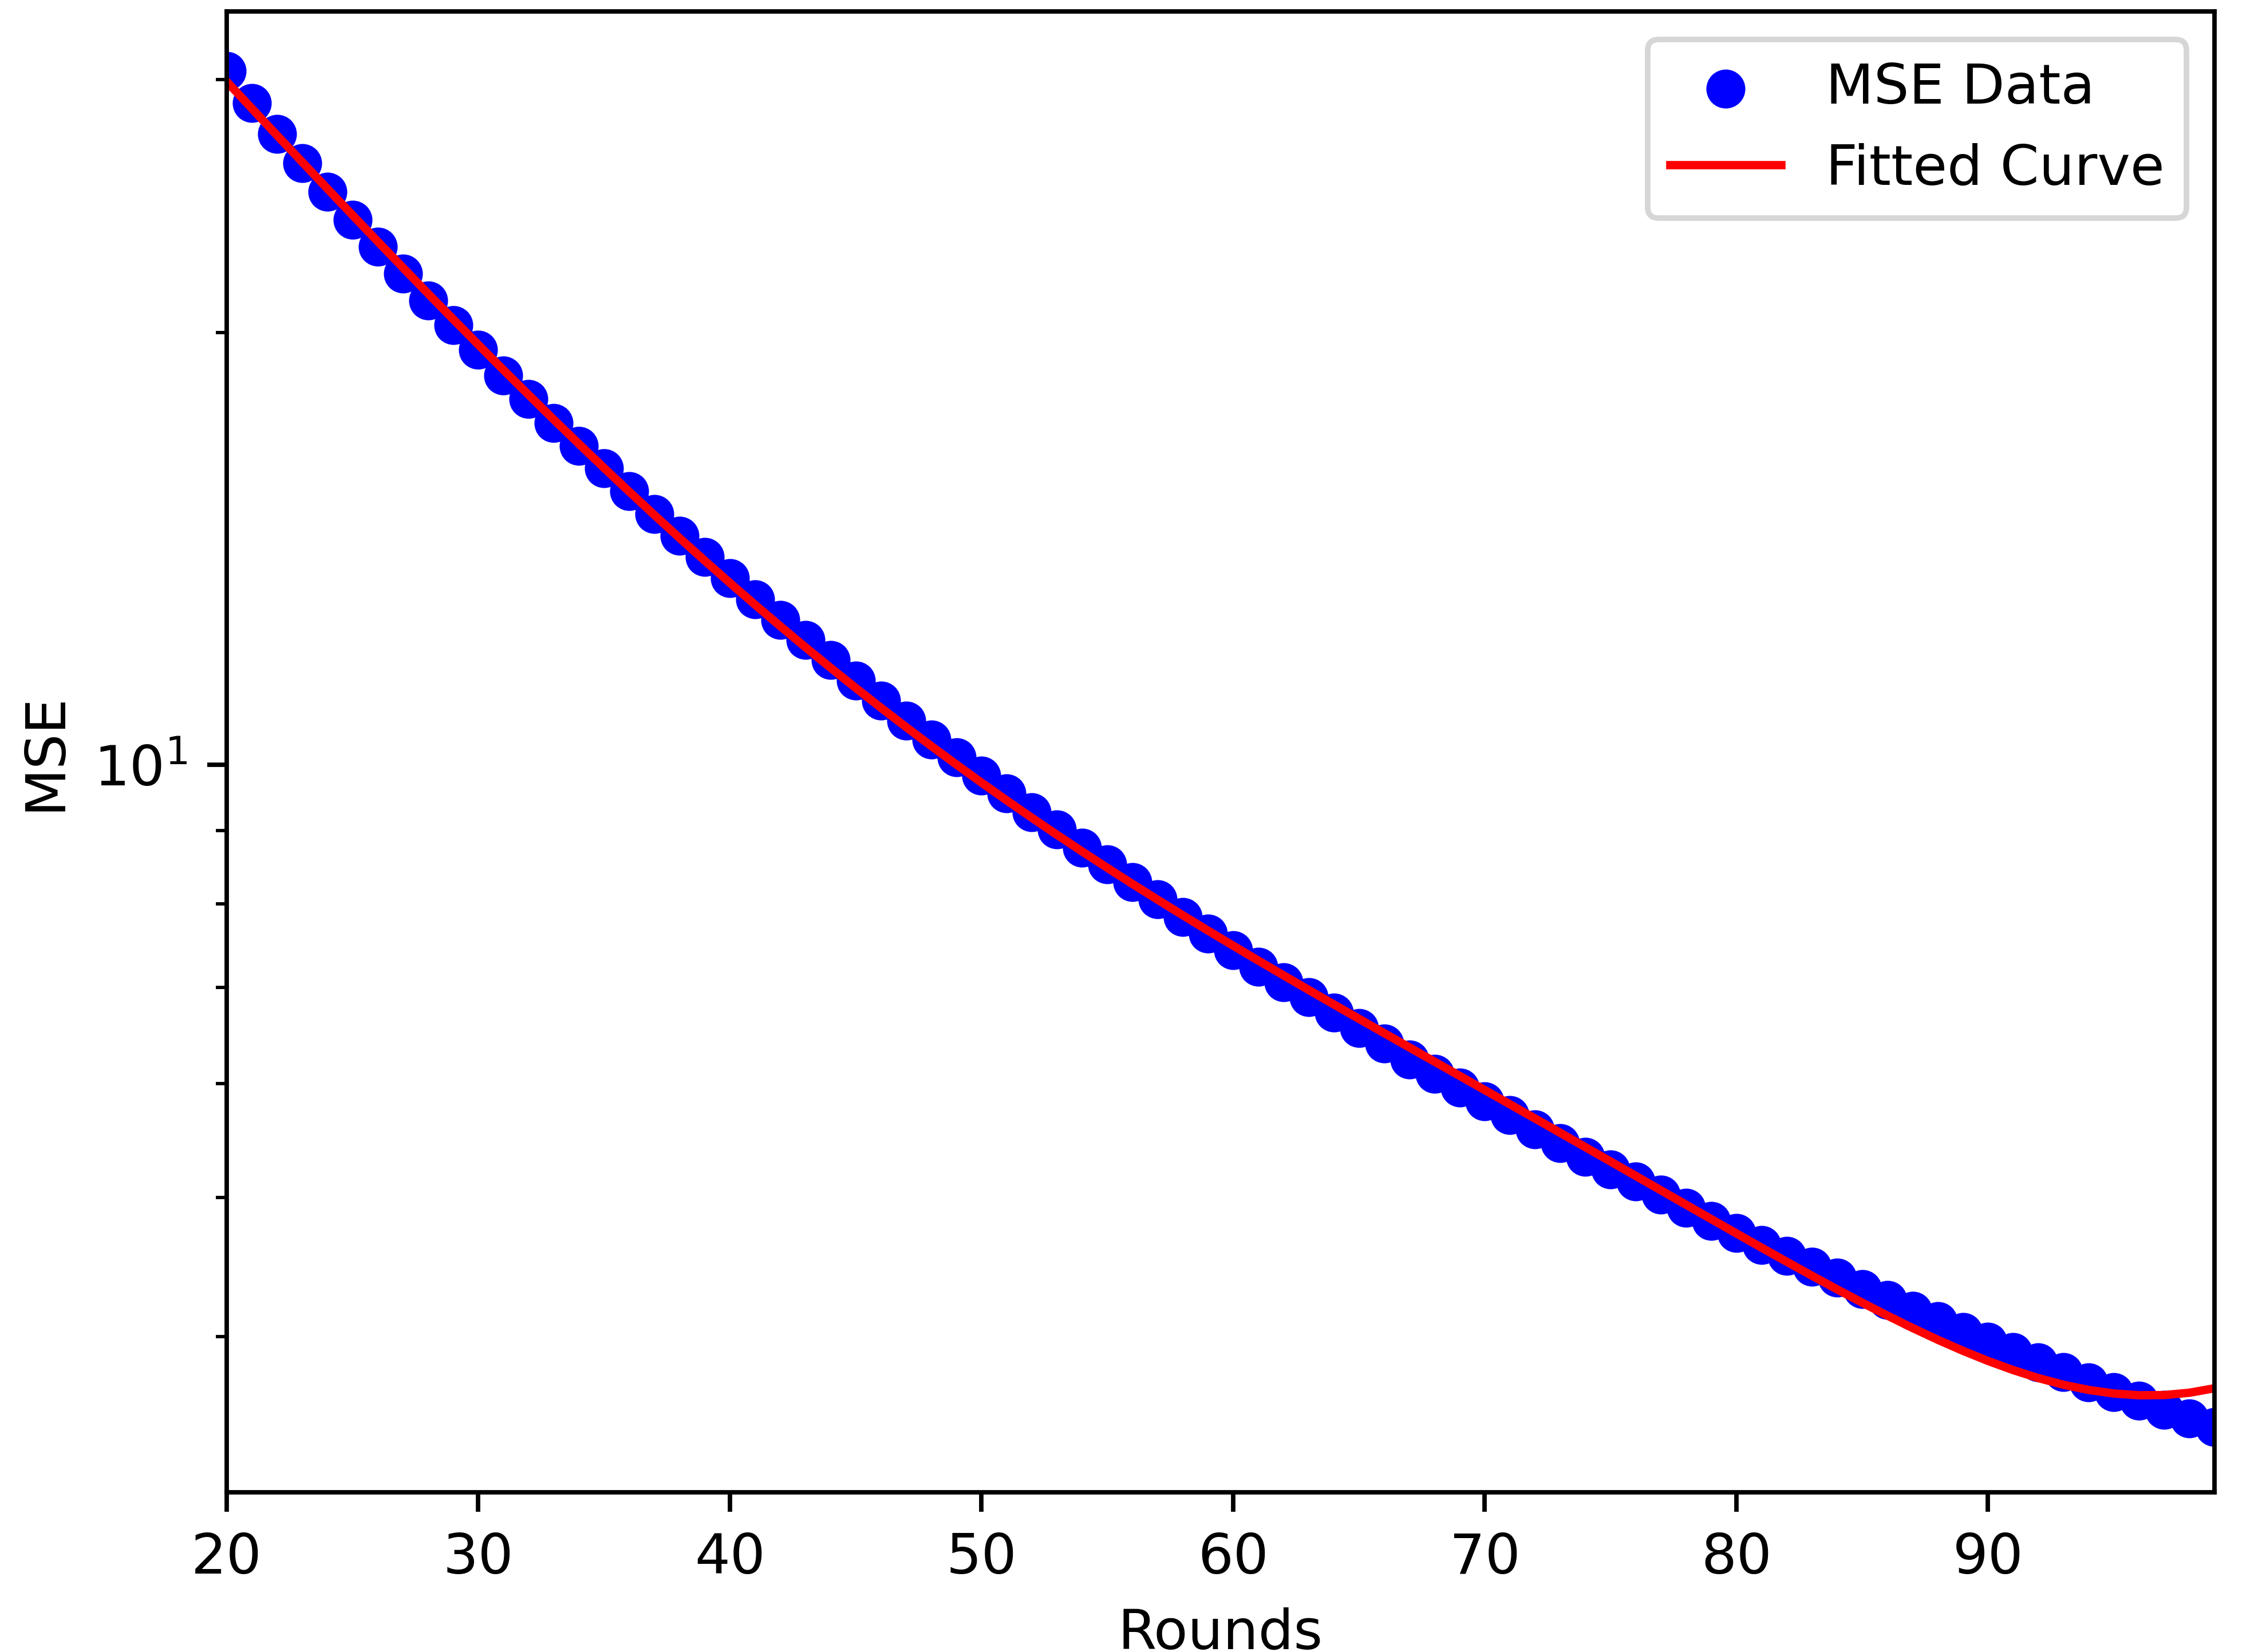
\includegraphics{figures/Simulation_outcomes/LollipopGraph/128_896/ATPPS/ATPPS_modelfitting_rounds_99_model_2.png}}
    \caption{(128, 896)-Lollipop graph - polynomial regression fit: ATPPS}
    \label{fig:atpps_128x896lollipopgraphModelFit}
\end{figure}

\begin{figure}
    \centering
    \scalebox{0.8}{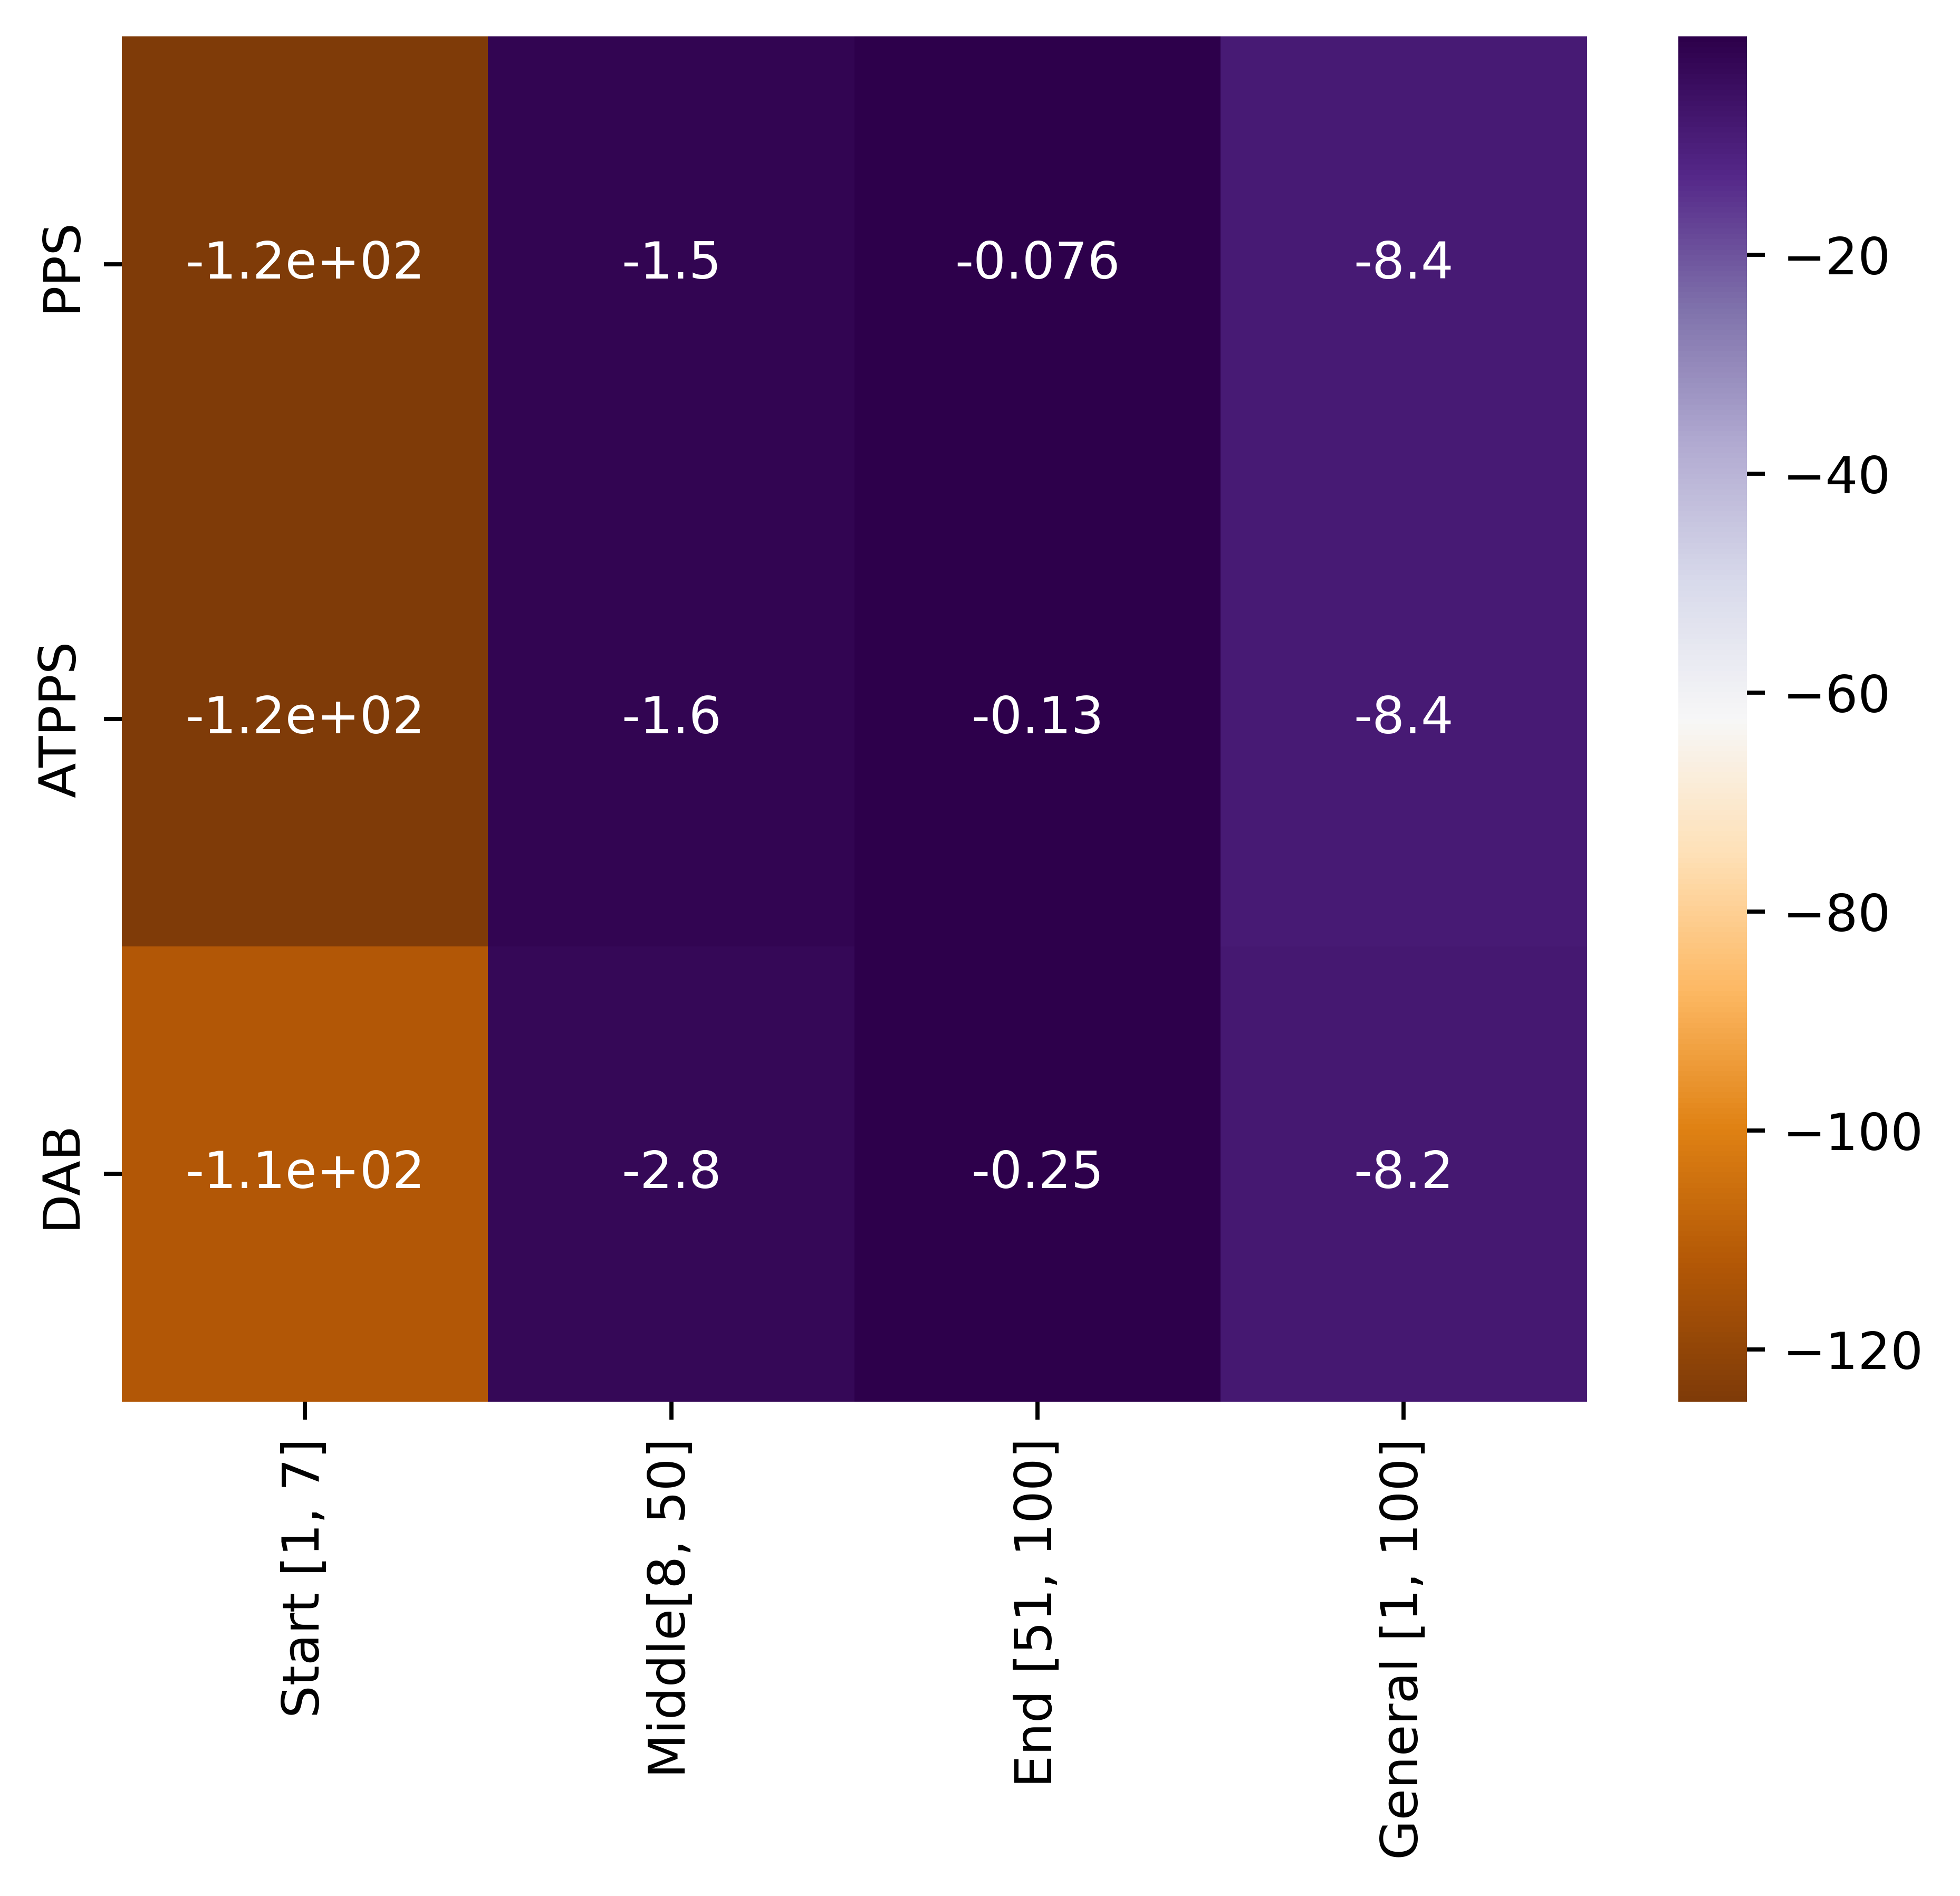
\includegraphics{figures/Simulation_outcomes/LollipopGraph/128_896/DAB_vs_PPS_vs_ATPPS_slopesheatmap_100rounds.png}}
    \caption{(128, 896)-Lollipop graph: heat map of slopes per region}
    \label{fig:128_896lollipopslopes}
\end{figure}

\subsection{(896, 128) Lollipop Graph}\label{subsec:896_128lollipop}
Now that more nodes are assigned to the clique and taken from the path compared to the initial experiment where the clique and the path had the same number of nodes, the discrepancy between the Push-Pull Sum based and the DAB algorithms is more obvious, as shown in figure \ref{fig:896_128lollipopgraphMSEperRoundLogLog}. This is also indicated by the slopes. In the start region the Push-Pull Sum based algorithms both balance the network with the (896, 128)-Lollipop graph more quickly, achieving slopes of -140 in this initial region, compared to -130 (figure \ref{fig:896x128lollipopslopes}) in the (512, 512)-Lollipop graph. The overall MSE is also lower for the (896, 128)-Lollipop graph, where the error is reduced to a value of 3.27 for the network where the ATPPS is applied and 3.59 for the network where PPS is applied as a load balancing strategy. The MSE values for the (512, 512)-Lollipop graph are higher, where the MSE data of the ATPPS shows values of 13.83 and for the PPS 14.71. However, no significant advantage of the ATPPS over the PPS is observed. The DAB struggles to achieve good performance in reducing error, showcased by the immense discrepancy between the MSE values after 100 rounds. For the (512, 512)-Lollipop graph experiments the DAB achieved values of 108.90, in the experiment of (896, 128)-Lollipop graph the value that the network ends up with is at 542.09, which is nearly five times as much.

The best-fit polynomials fitted to the MSE data of the load balancing algorithms are of degree 3 for the DAB MSE data and of degree 4 for the PPS-based algorithms MSE data. The polynomial for the DAB MSE data follows the equation: $MSE_r=-1.936\times 10^{-4}r^{3}+0.05r^{2}-5.33r+745.95$ (figure \ref{fig:dab_896x128lollipopgraphModelFit}). The polynomial for the Push-Pull Sum based algorithms follow the equation: $MSE_r=2.00\times 10^{-7}r^{4}-6.01\times 10^{-5}r^{3}+6.95\times 10^{-3}r^{2}-0.39r+13.44$ (figure \ref{fig:pps_896x128lollipopgraphModelFit}) for the PPS and $MSE_r=2.28\times 10^{-7}r^{4}-6.77\times 10^{-5}r^{3}+7.68\times 10^{-3}r^{2}-0.42r+13.62$ for the ATPPS (figure \ref{fig:atpps_896x128lollipopgraphModelFit}). 
\begin{figure}[]
    \centering
    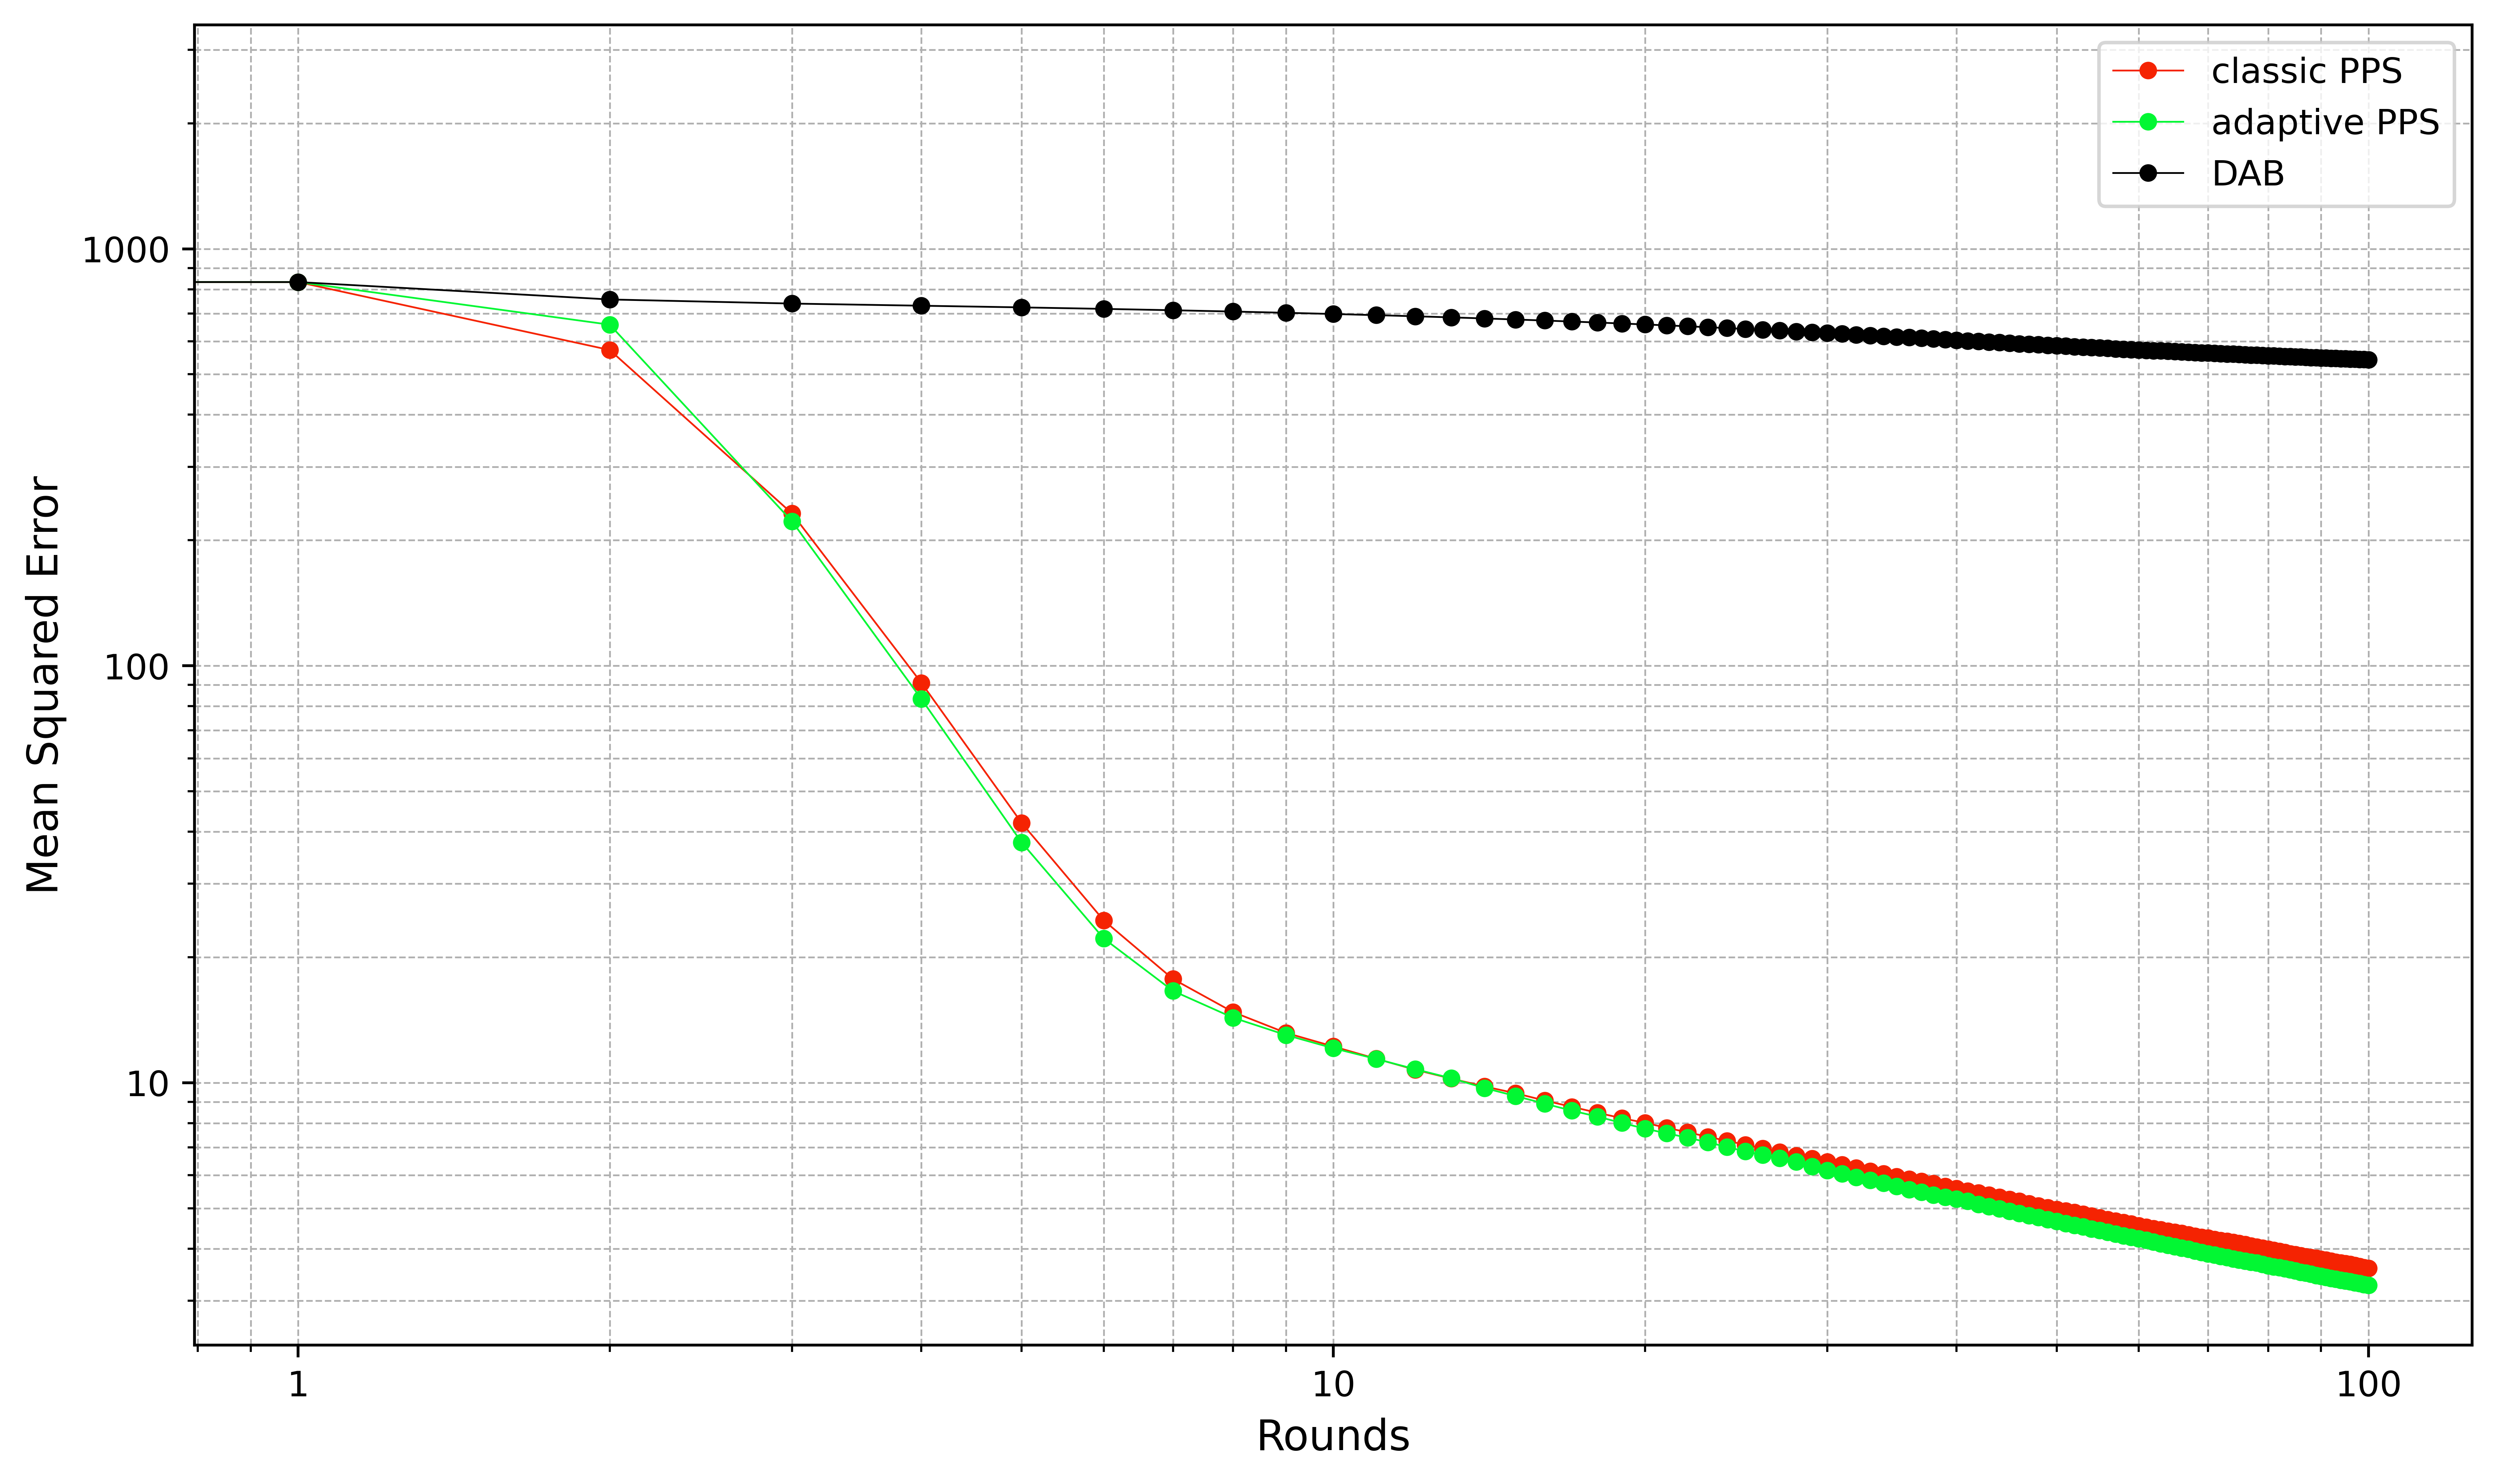
\includegraphics[width=\linewidth]{figures/Simulation_outcomes/LollipopGraph/896_128/DAB_vs_PPS_LG_r100_n1024_averaged_loglog.png}
    \caption{(896, 128)-Lollipop graph: mean squared error per rounds (log-log)}
    \label{fig:896_128lollipopgraphMSEperRoundLogLog}
\end{figure}

\begin{figure}[]
    \centering
    \scalebox{0.8}{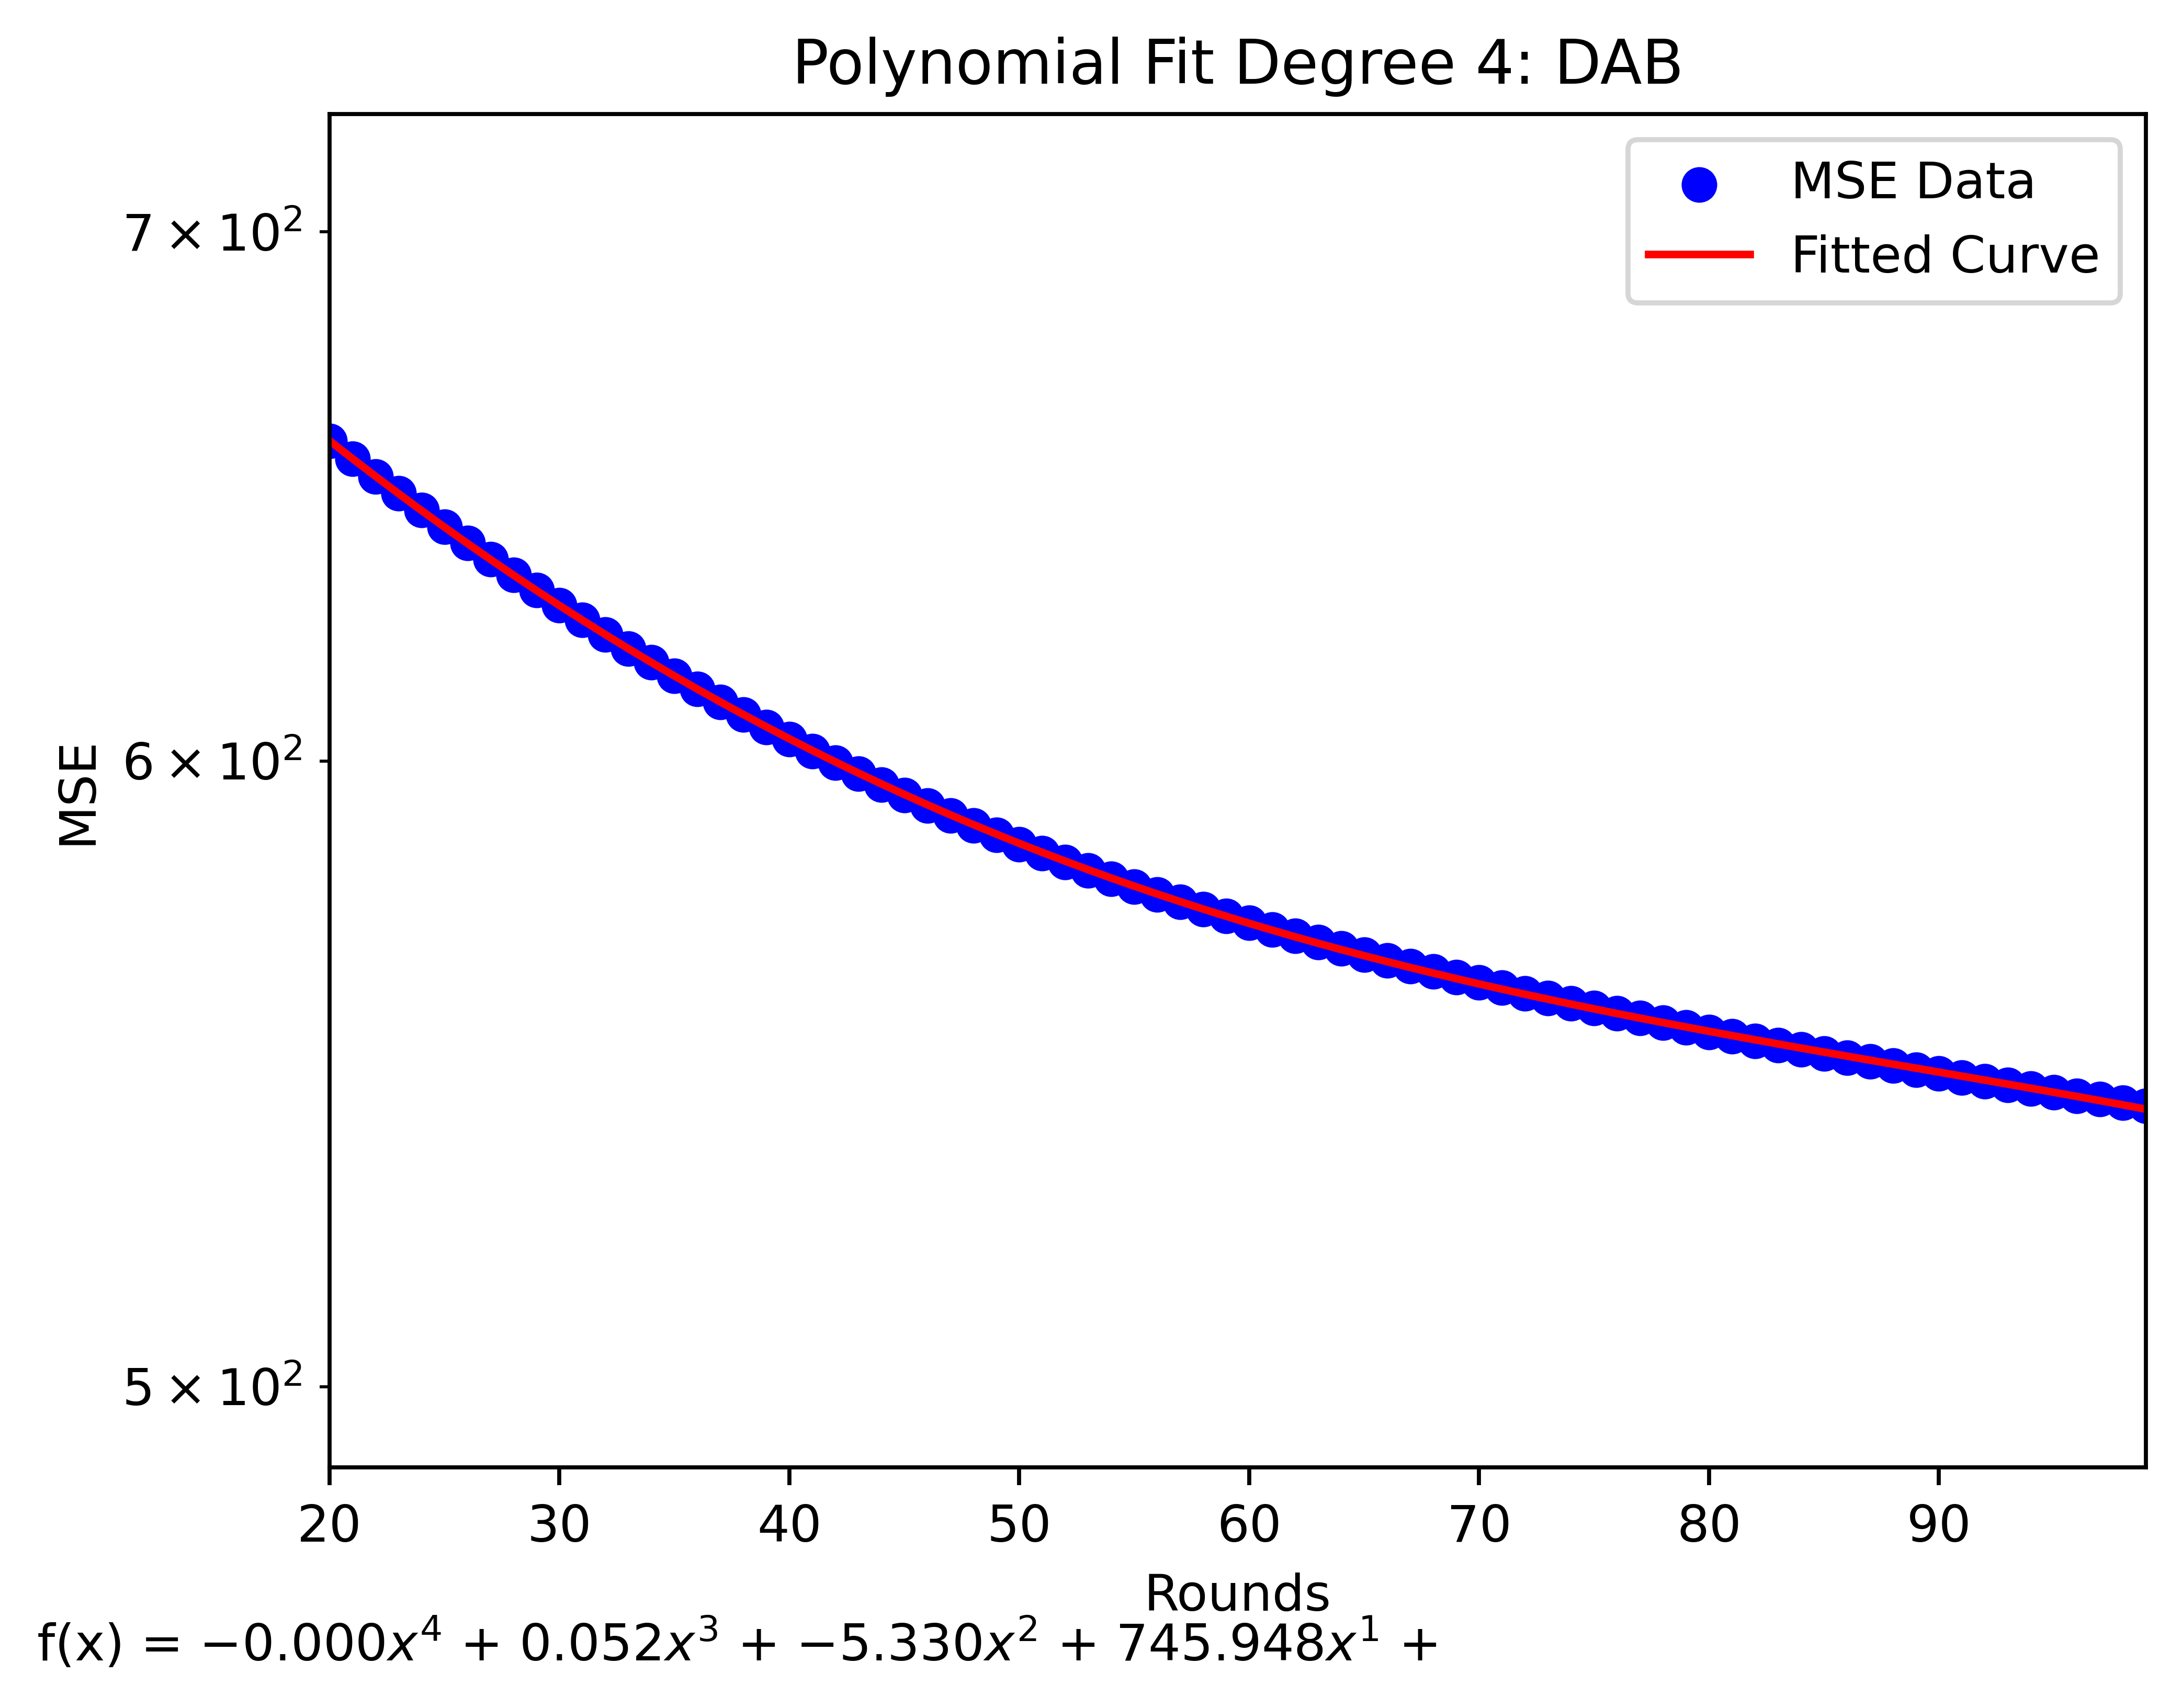
\includegraphics[width=\linewidth]{figures/Simulation_outcomes/LollipopGraph/896_128/DAB/DAB_modelfitting_rounds_99_model_2.png}}
    \caption{(896, 128)-Lollipop graph - polynomial regression fit: DAB}
    \label{fig:dab_896x128lollipopgraphModelFit}
\end{figure}

\begin{figure}[]
    \centering
    \scalebox{0.8}{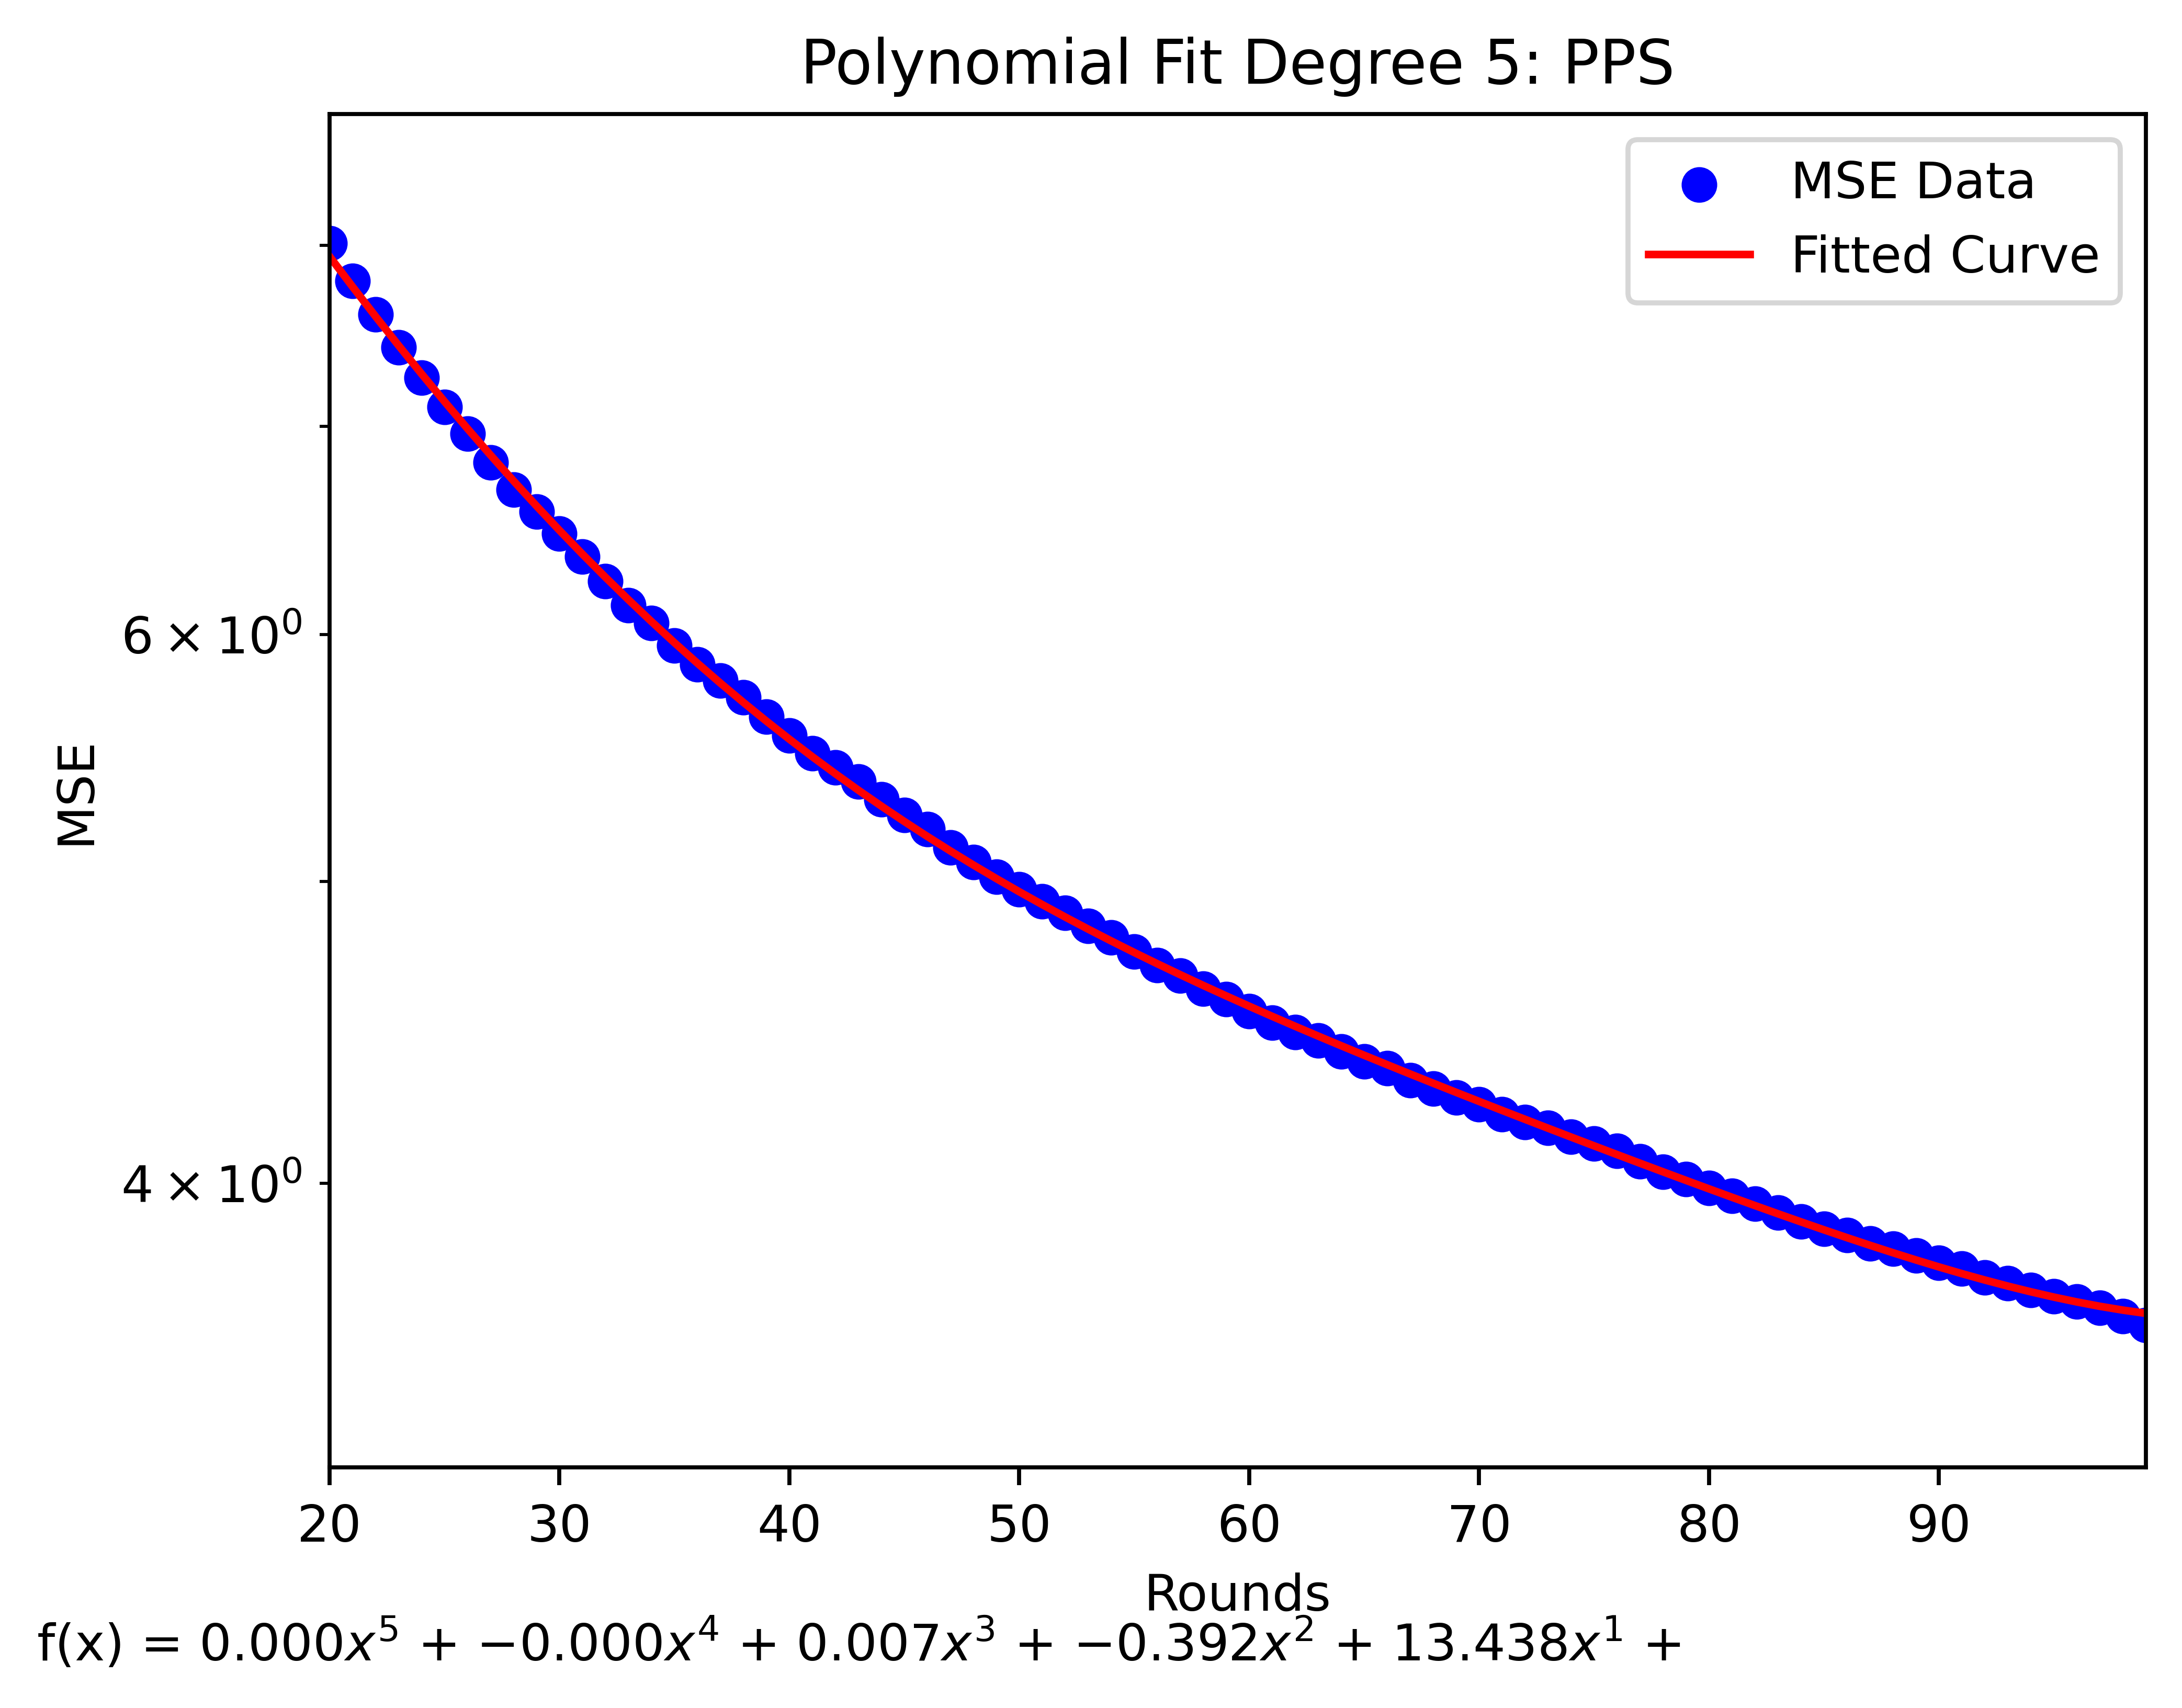
\includegraphics{figures/Simulation_outcomes/LollipopGraph/896_128/PPS/PPS_modelfitting_rounds_99_model_2.png}}
    \caption{(896, 128)-Lollipop graph - polynomial regression fit: PPS}
    \label{fig:pps_896x128lollipopgraphModelFit}
\end{figure}

\begin{figure}[]
    \centering
    \scalebox{0.8}{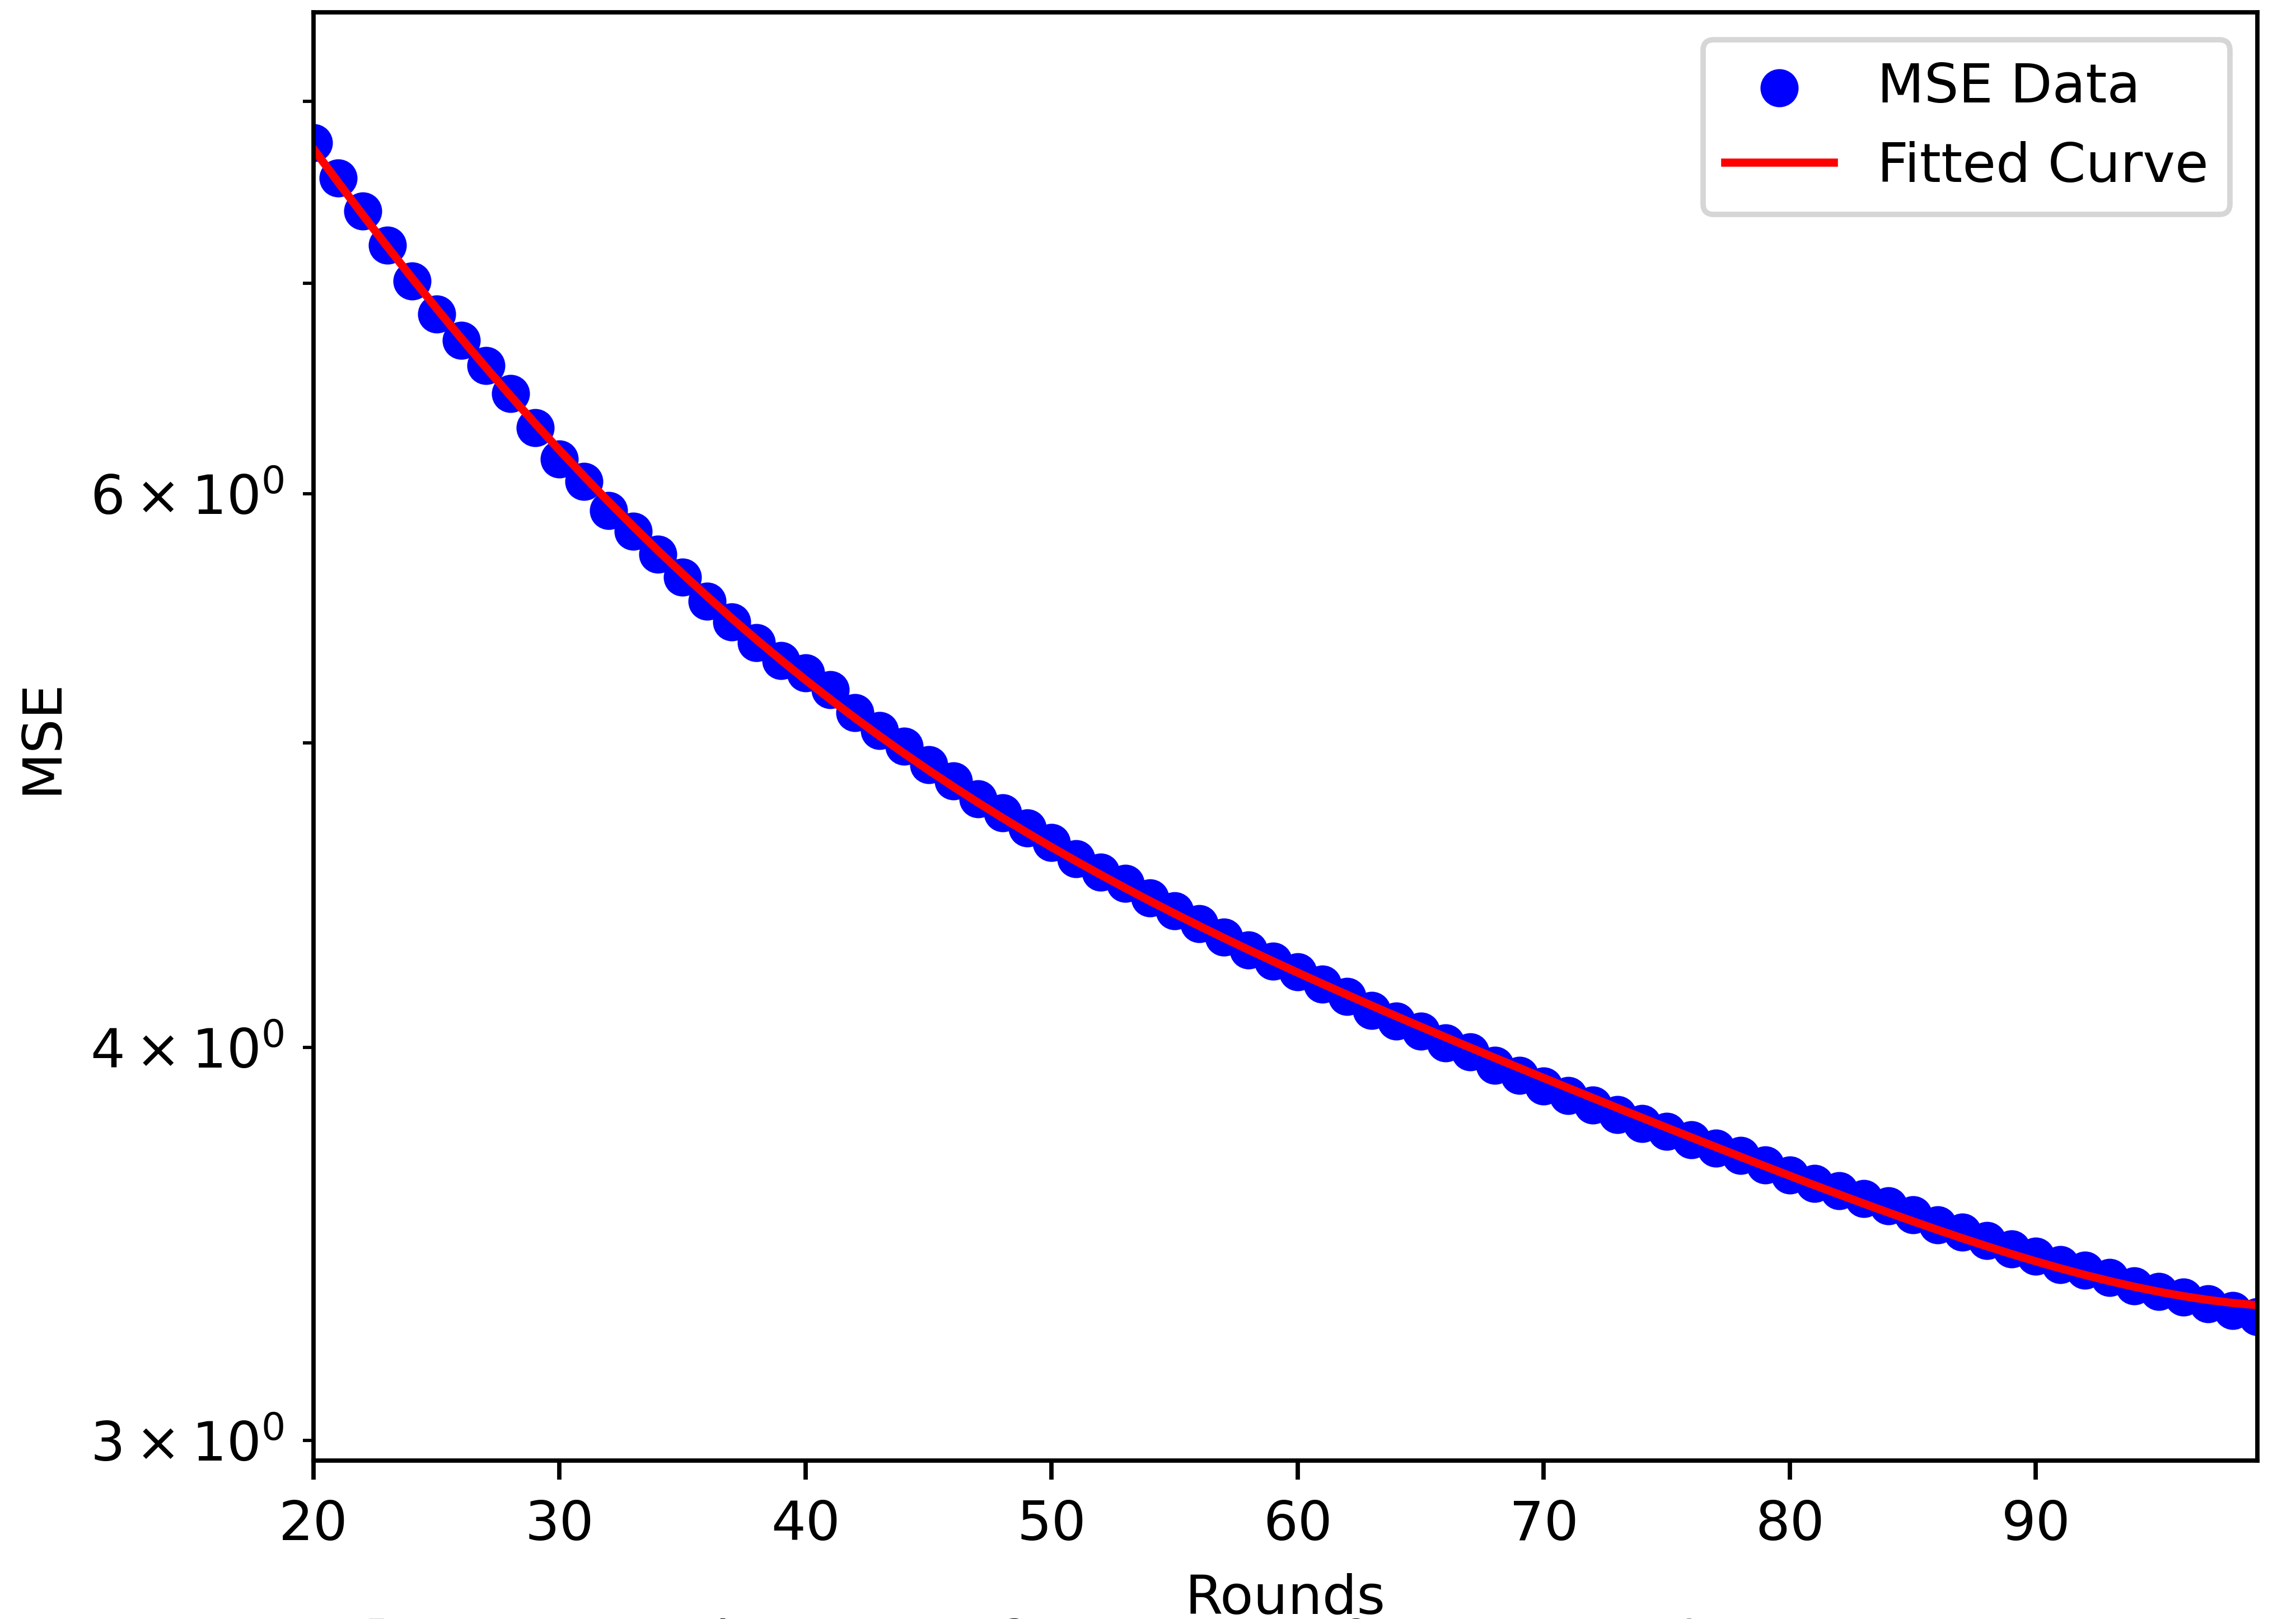
\includegraphics[width=\linewidth]{figures/Simulation_outcomes/LollipopGraph/896_128/ATPPS/ATPPS_modelfitting_rounds_99_model_2.png}}
    \caption{(896, 128)-Lollipop graph - polynomial regression fit: ATPPS}
    \label{fig:atpps_896x128lollipopgraphModelFit}
\end{figure}

\begin{figure}
    \centering
    \scalebox{0.8}{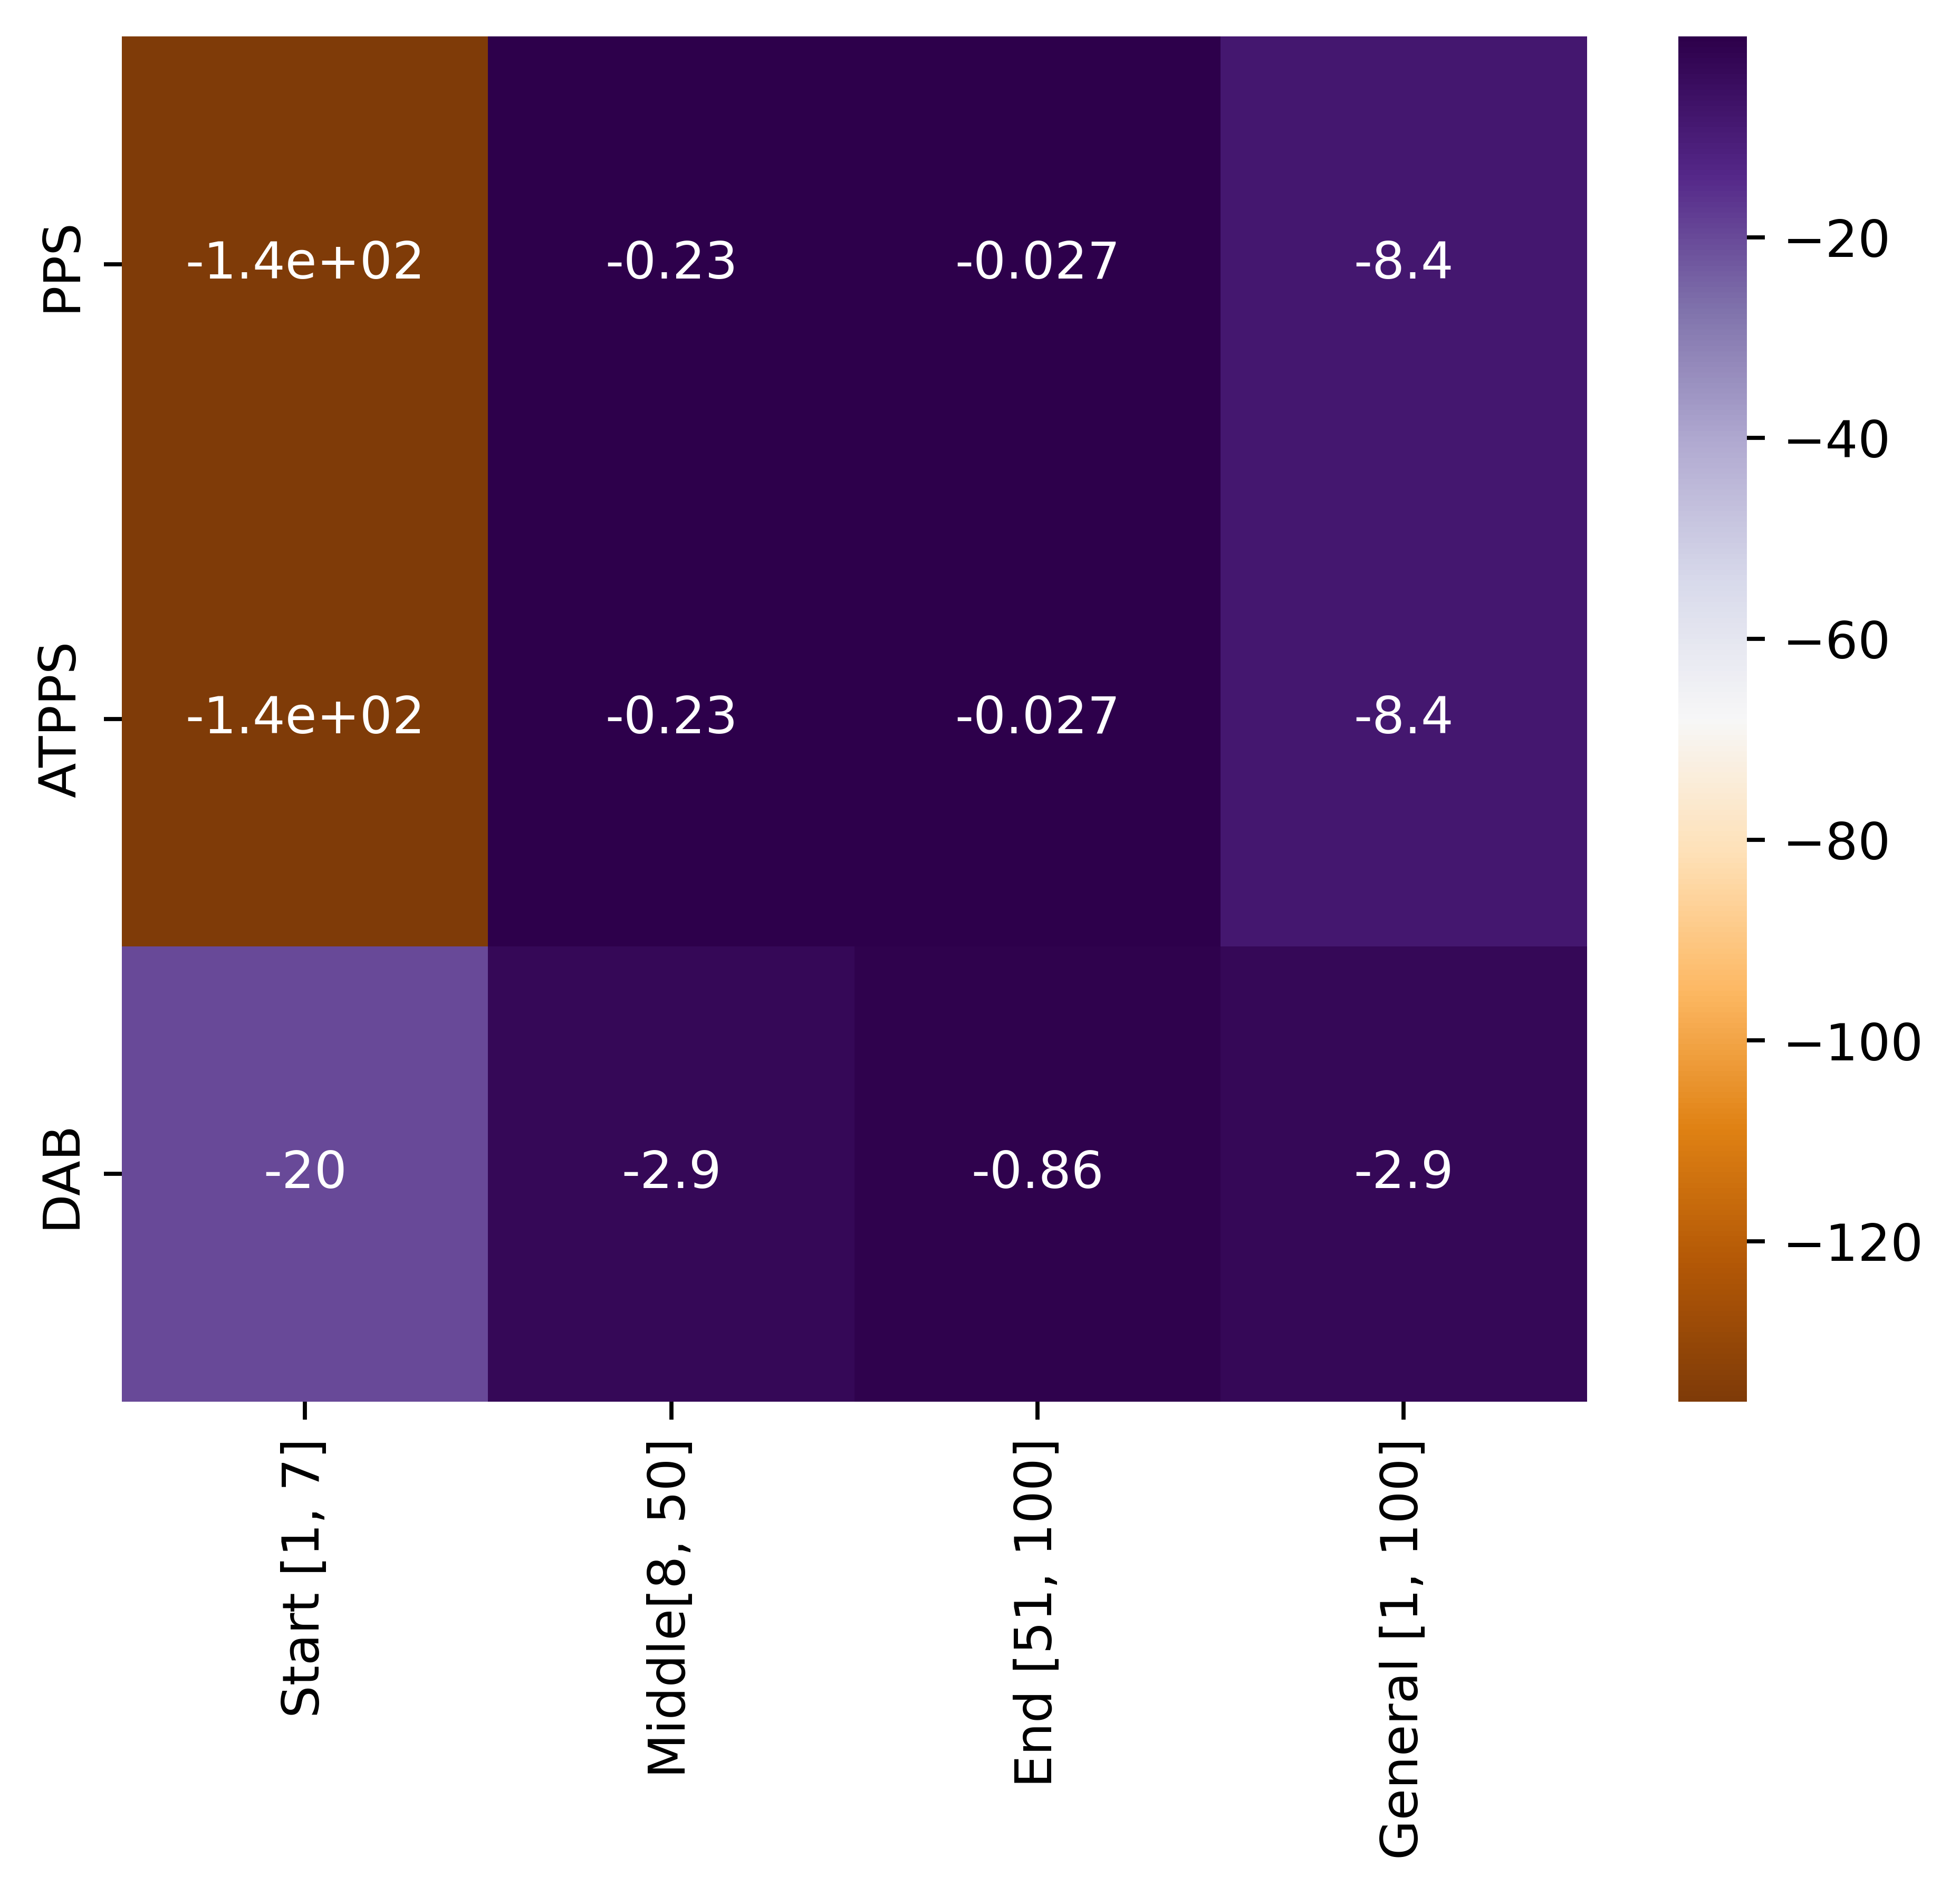
\includegraphics{figures/Simulation_outcomes/LollipopGraph/896_128/DAB_vs_PPS_vs_ATPPS_slopesheatmap_100rounds.png}}
    \caption{(896, 128) Lollipop Graph: heat map of slopes per region}
    \label{fig:896x128lollipopslopes}
\end{figure}

\section{Ring of Cliques}\label{sec:ringofcliques}
\subsection{32x32 Ring of Cliques}\label{subsec:32_32ROC}
In the early rounds, PPS and ATPPS exhibit the fastest MSE reduction showcased by a very steep downwards trend between rounds 1 and 5 in figure \ref{fig:atppsRingOfCliquesLog_LogLog} b). Both Push-Pull Sum based approaches start with faster convergence rates compared to DAB. The initial steep downwards slope of -200 for each Push-Pull Sum based algorithm as depicted in figure \ref{fig:ringOfCliquesslopes} within the first 5 rounds is due to the unbalanced state of each clique. The Push-Pull Sum based approaches have shown to be outperforming the DAB algorithm for Complete graphs. While the cliques are still unbalanced the Push-Pull Sum based algorithms achieve faster convergence. After the cliques are balanced round by round the DAB algorithm catches up especially between the rounds 6 to 40 where the slopes are -48 compared to $\sim-2$ for the Push-Pull Sum based algorithms. Nodes within cliques tend to converge quickly internally due to their dense interconnections for the Push-Pull Sum based algorithms. However, load balancing between cliques, especially when the nodes select for random neighbors is slower, creating bottlenecks for global convergence (this is especially the case for the PPS, whichs curve starts to stagnate between round 10 to 100). Due to the determistic nature of the DAB, the bridging nodes choose nodes outside of their cliques, once the load is balanced within the clique, and spread the load to other cliques. The ATPPS algorithm achieves better results compared to the PPS, since it has a similar mechanism in this scenario like the DAB, prioritizing communication between cliques (where differences in loads are more significant) over redundant communication within cliques (where loads are already close to balanced). This is mirrored in the behavior of the curve after round 10. Again, the ATPPS acts as a compromise solution between the PPS and the DAB achieving results close to them of the DAB algorithm. Overall, at round 100 the DAB achieved a MSE of $\sim 6.55$, the PPS a MSE of 19.80 and the ATPPS a MSE of 8.42.

The polynomial fit for the DAB algorithm is: $MSE_r=1.04\times 10^{-6}r^{4}-2.941\times 10^{-4}r^{3}+0.03r^{2}-1.66r+45.30$ (figure \ref{fig:dabRingOfCliquesModelFit}). Thus the MSE as a function of rounds is modeled by a fourth degree polynomial. The PPS MSE data of rounds 20 to 100 is fitted to a linear regression model following the equation: $MSE_r=-0.05r+24.70$ (figure \ref{fig:ppsRingOfCliquesModelFit}). The negative slope indicates a consistent reduction in MSE with each round in this region, but the value -0.05 is relatively small. This suggests that the PPS algorithm achieves slow and steady progress toward load balancing. The linear fit highlights that PPS achieves only gradual improvement in balancing the load in the Ring of Cliques topology. The reason for that is that PPS focuses on a push-pull mechanism that is, relying on random neighbor interactions. In the Ring of Cliques, inter-clique connections are sparse, and PPS lacks a mechanism to prioritize balancing between these sparsely connected regions. As a result, its performance is bottlenecked by the topology. The linearity of the model suggests a uniform rate of error reduction across rounds, without any acceleration observed in other methods (like DAB). The logarithmic model for the ATPPS algorithm is given as:
$\log{(MSE_r)}=-7.59\log{(r)}+43.26$ (figure \ref{fig:atppsRingOfCliquesModelFit}). By exponentiating this equation, the relationship between the MSE and the number of rounds is: $MSE_r=10^{43.26}*r-7.59$. The steep negative slope of value -7.59 in the log-log fit indicates a rapid decrease in MSE as the number of rounds increases. This suggests that ATPPS achieves exponentially faster convergence compared to PPS, especially in the early rounds of load balancing.

\begin{figure}[!ht]
    \centering
        \subfloat[]{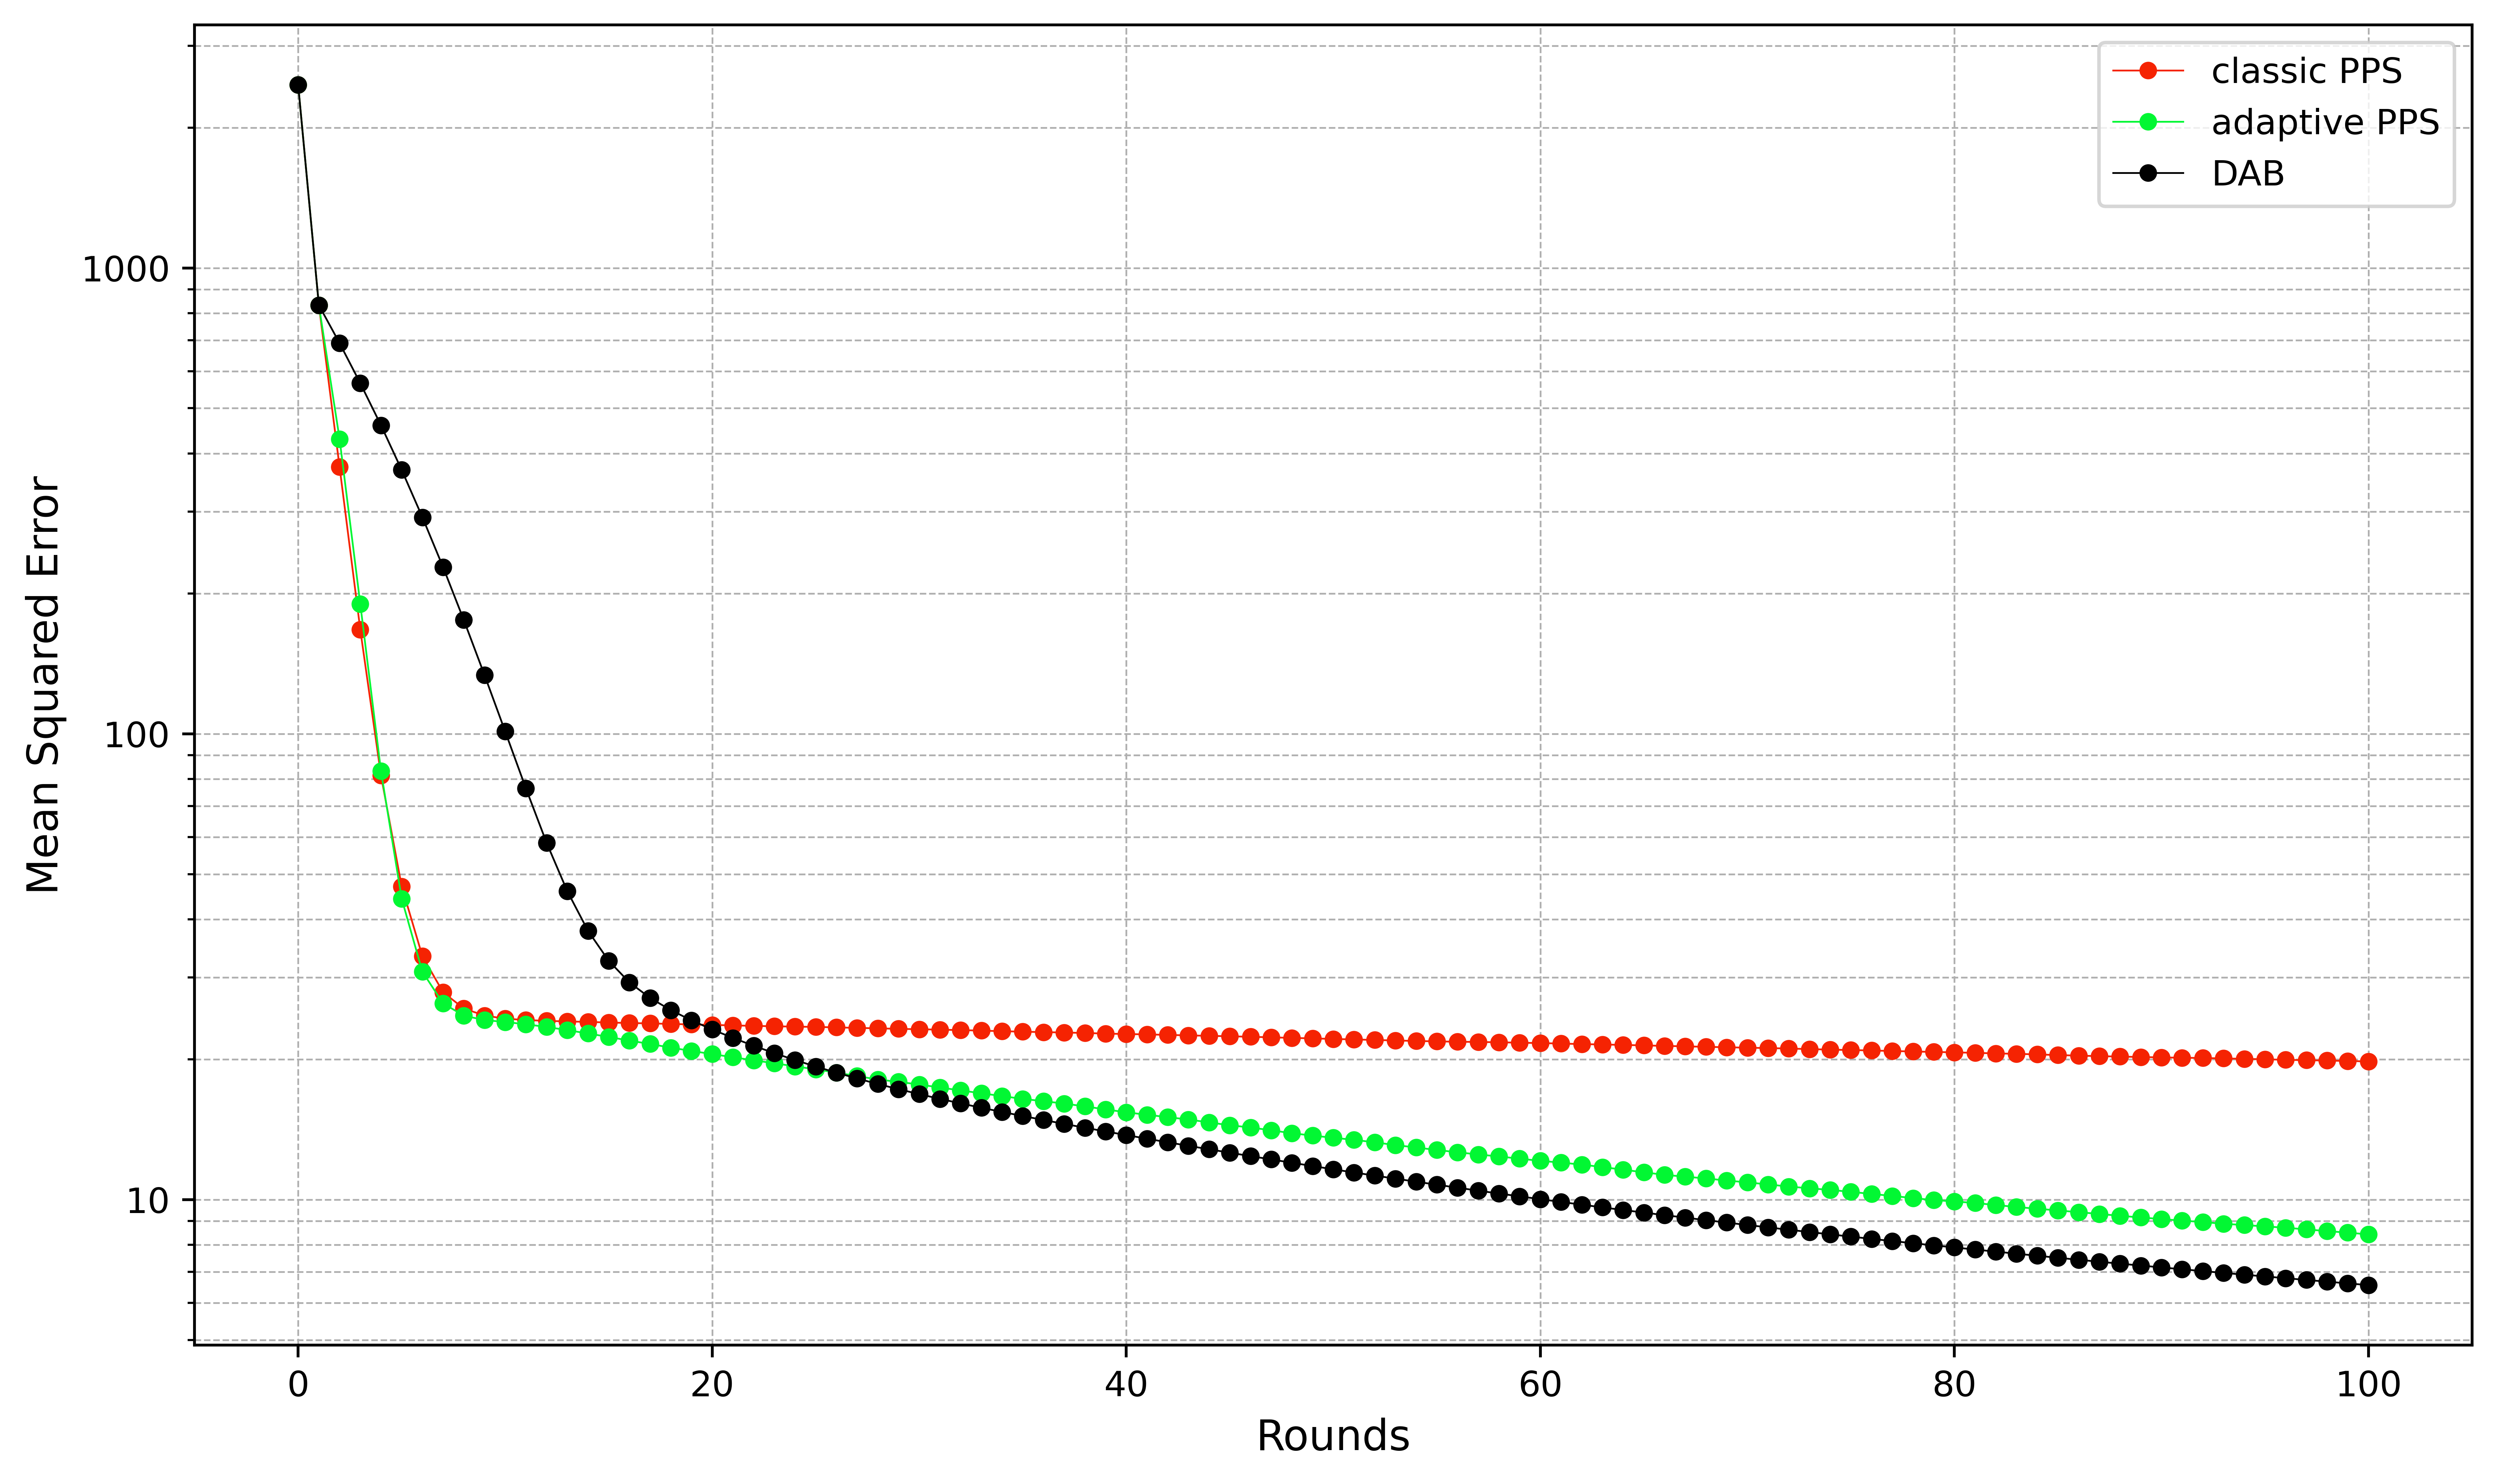
\includegraphics[width=0.49\linewidth]{figures/Simulation_outcomes/RingOfCliques/32x32/DAB_vs_PPS_RoC_r100_n1024_averaged_log.png}}
    \hfil
        \subfloat[]{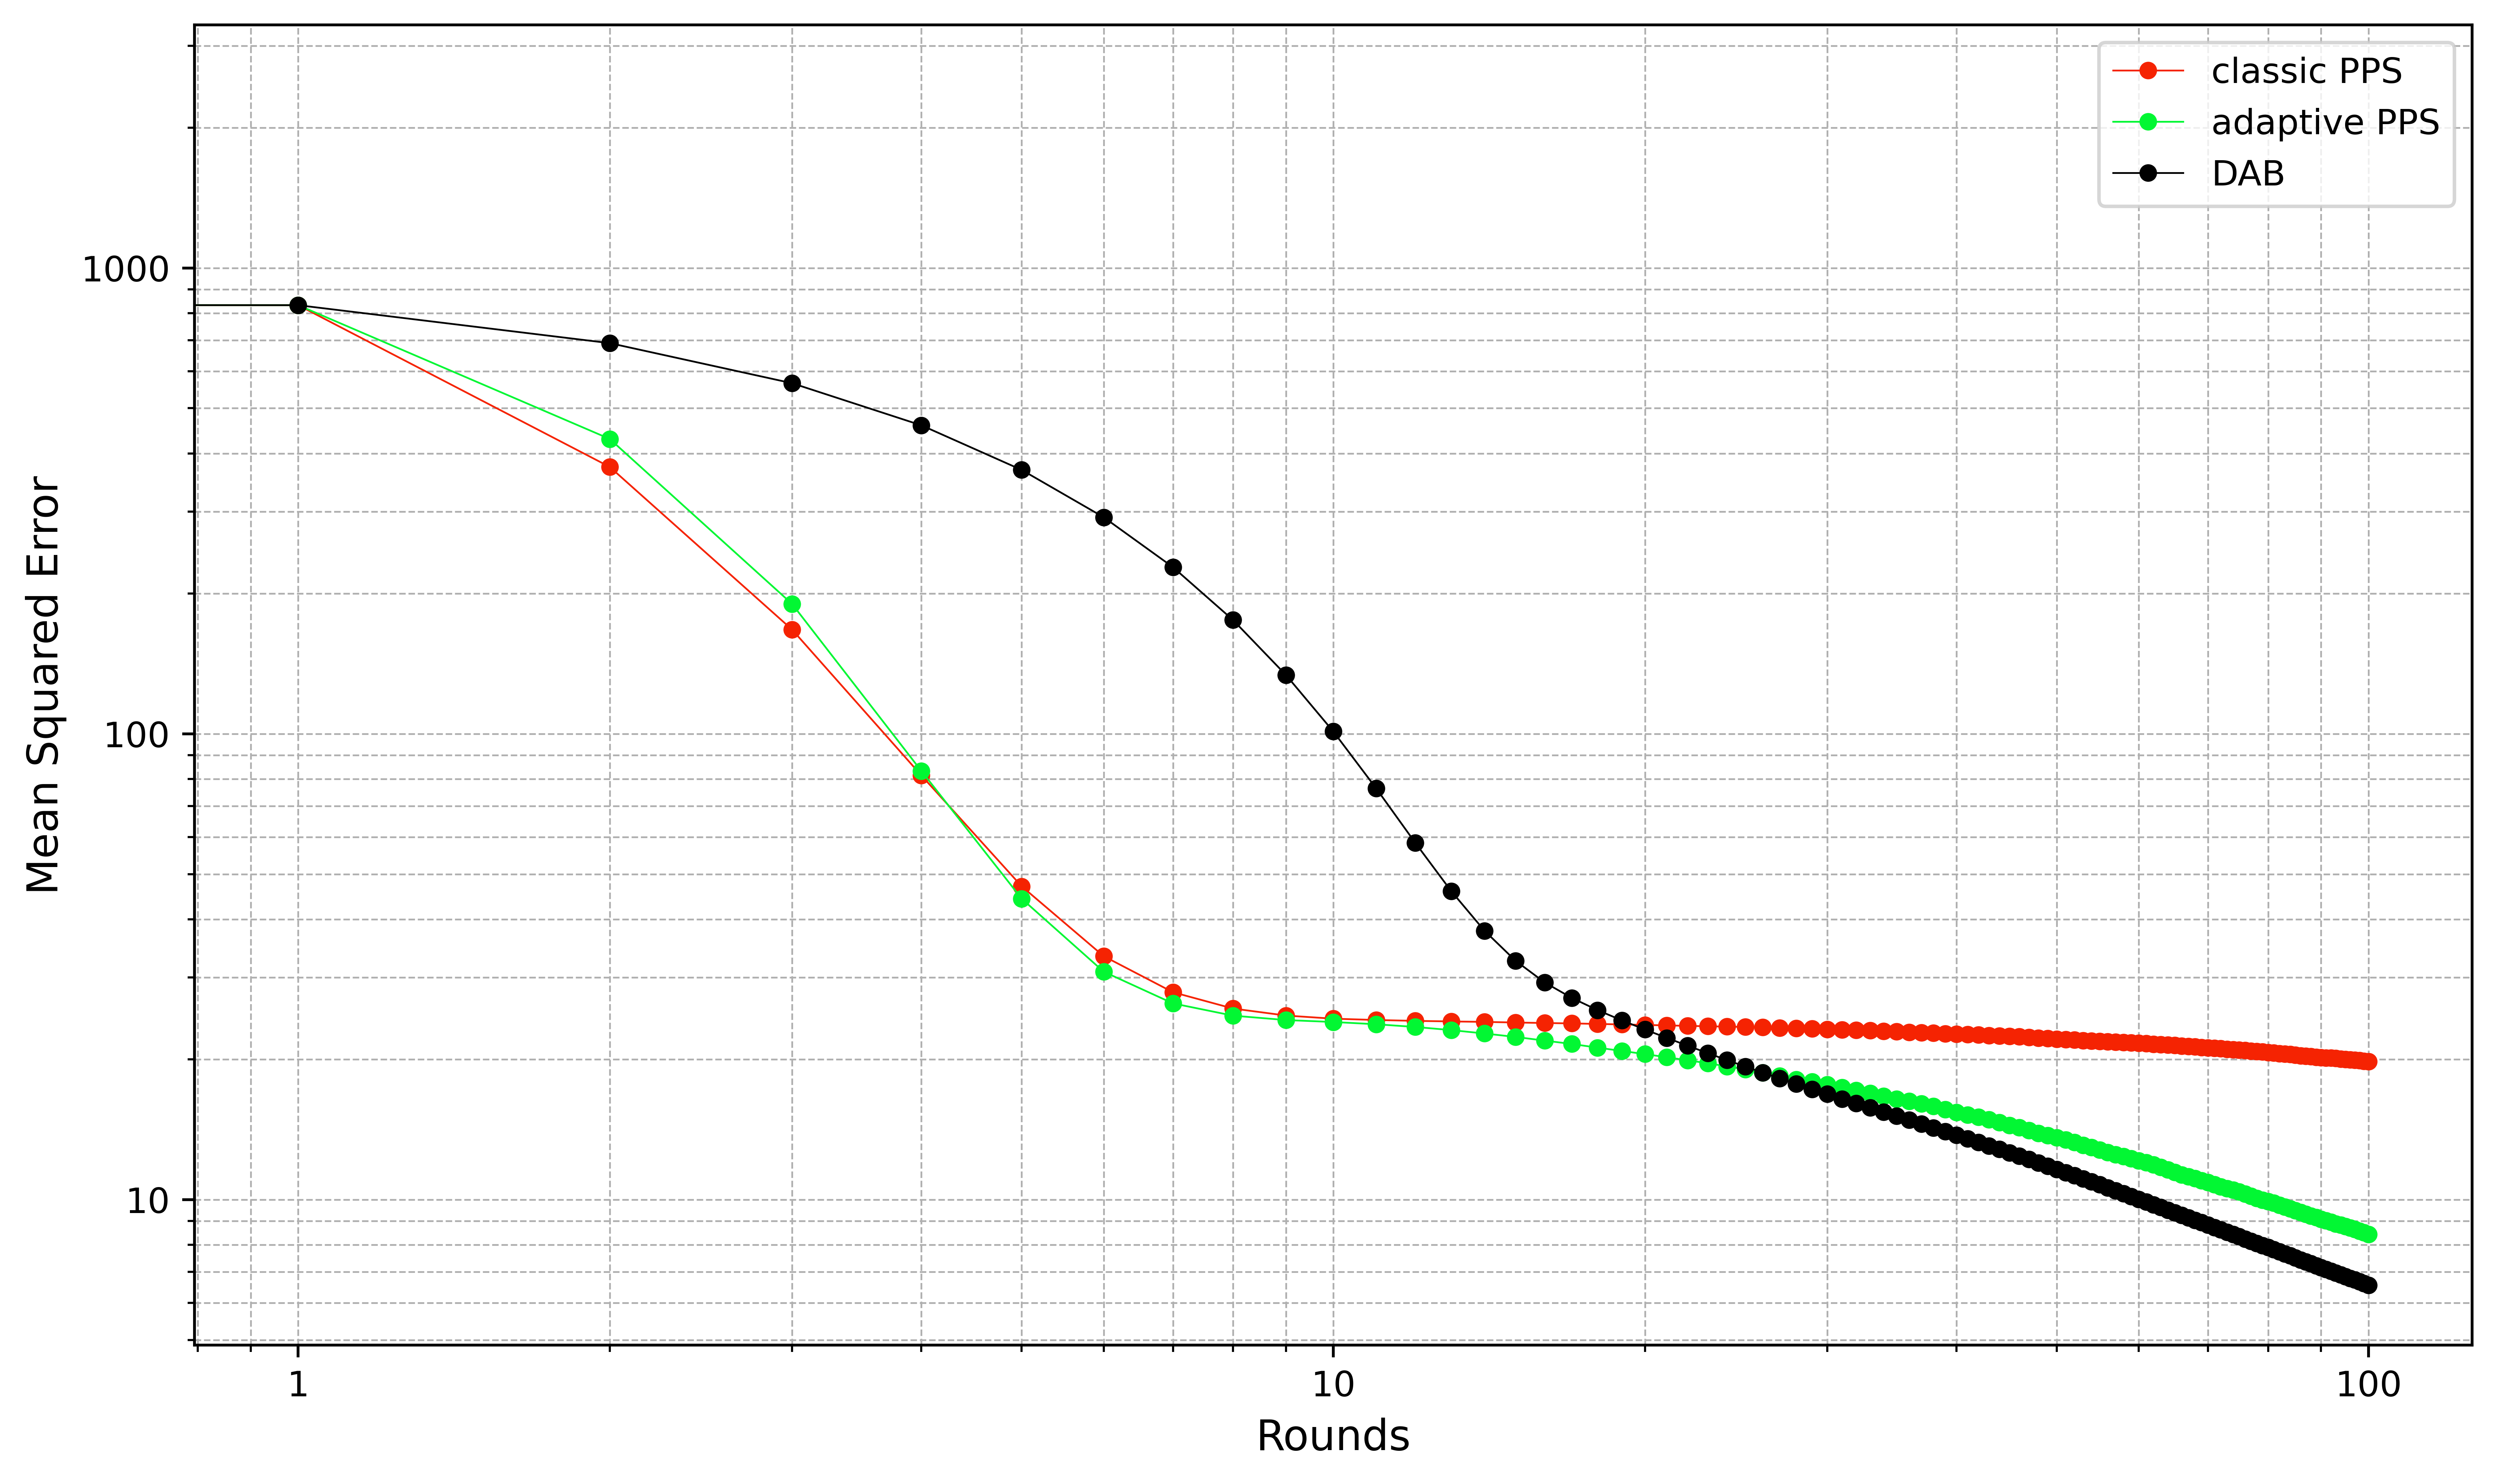
\includegraphics[width=0.49\linewidth]{figures/Simulation_outcomes/RingOfCliques/32x32/DAB_vs_PPS_RoC_r100_n1024_averaged_loglog.png}}
    \caption{$(32\times32)$-Ring of Cliques: mean squared error per rounds (log-linear and log-log)}
        \label{fig:atppsRingOfCliquesLog_LogLog}
\end{figure}
 \begin{figure}[]
     \centering
     \scalebox{0.8}{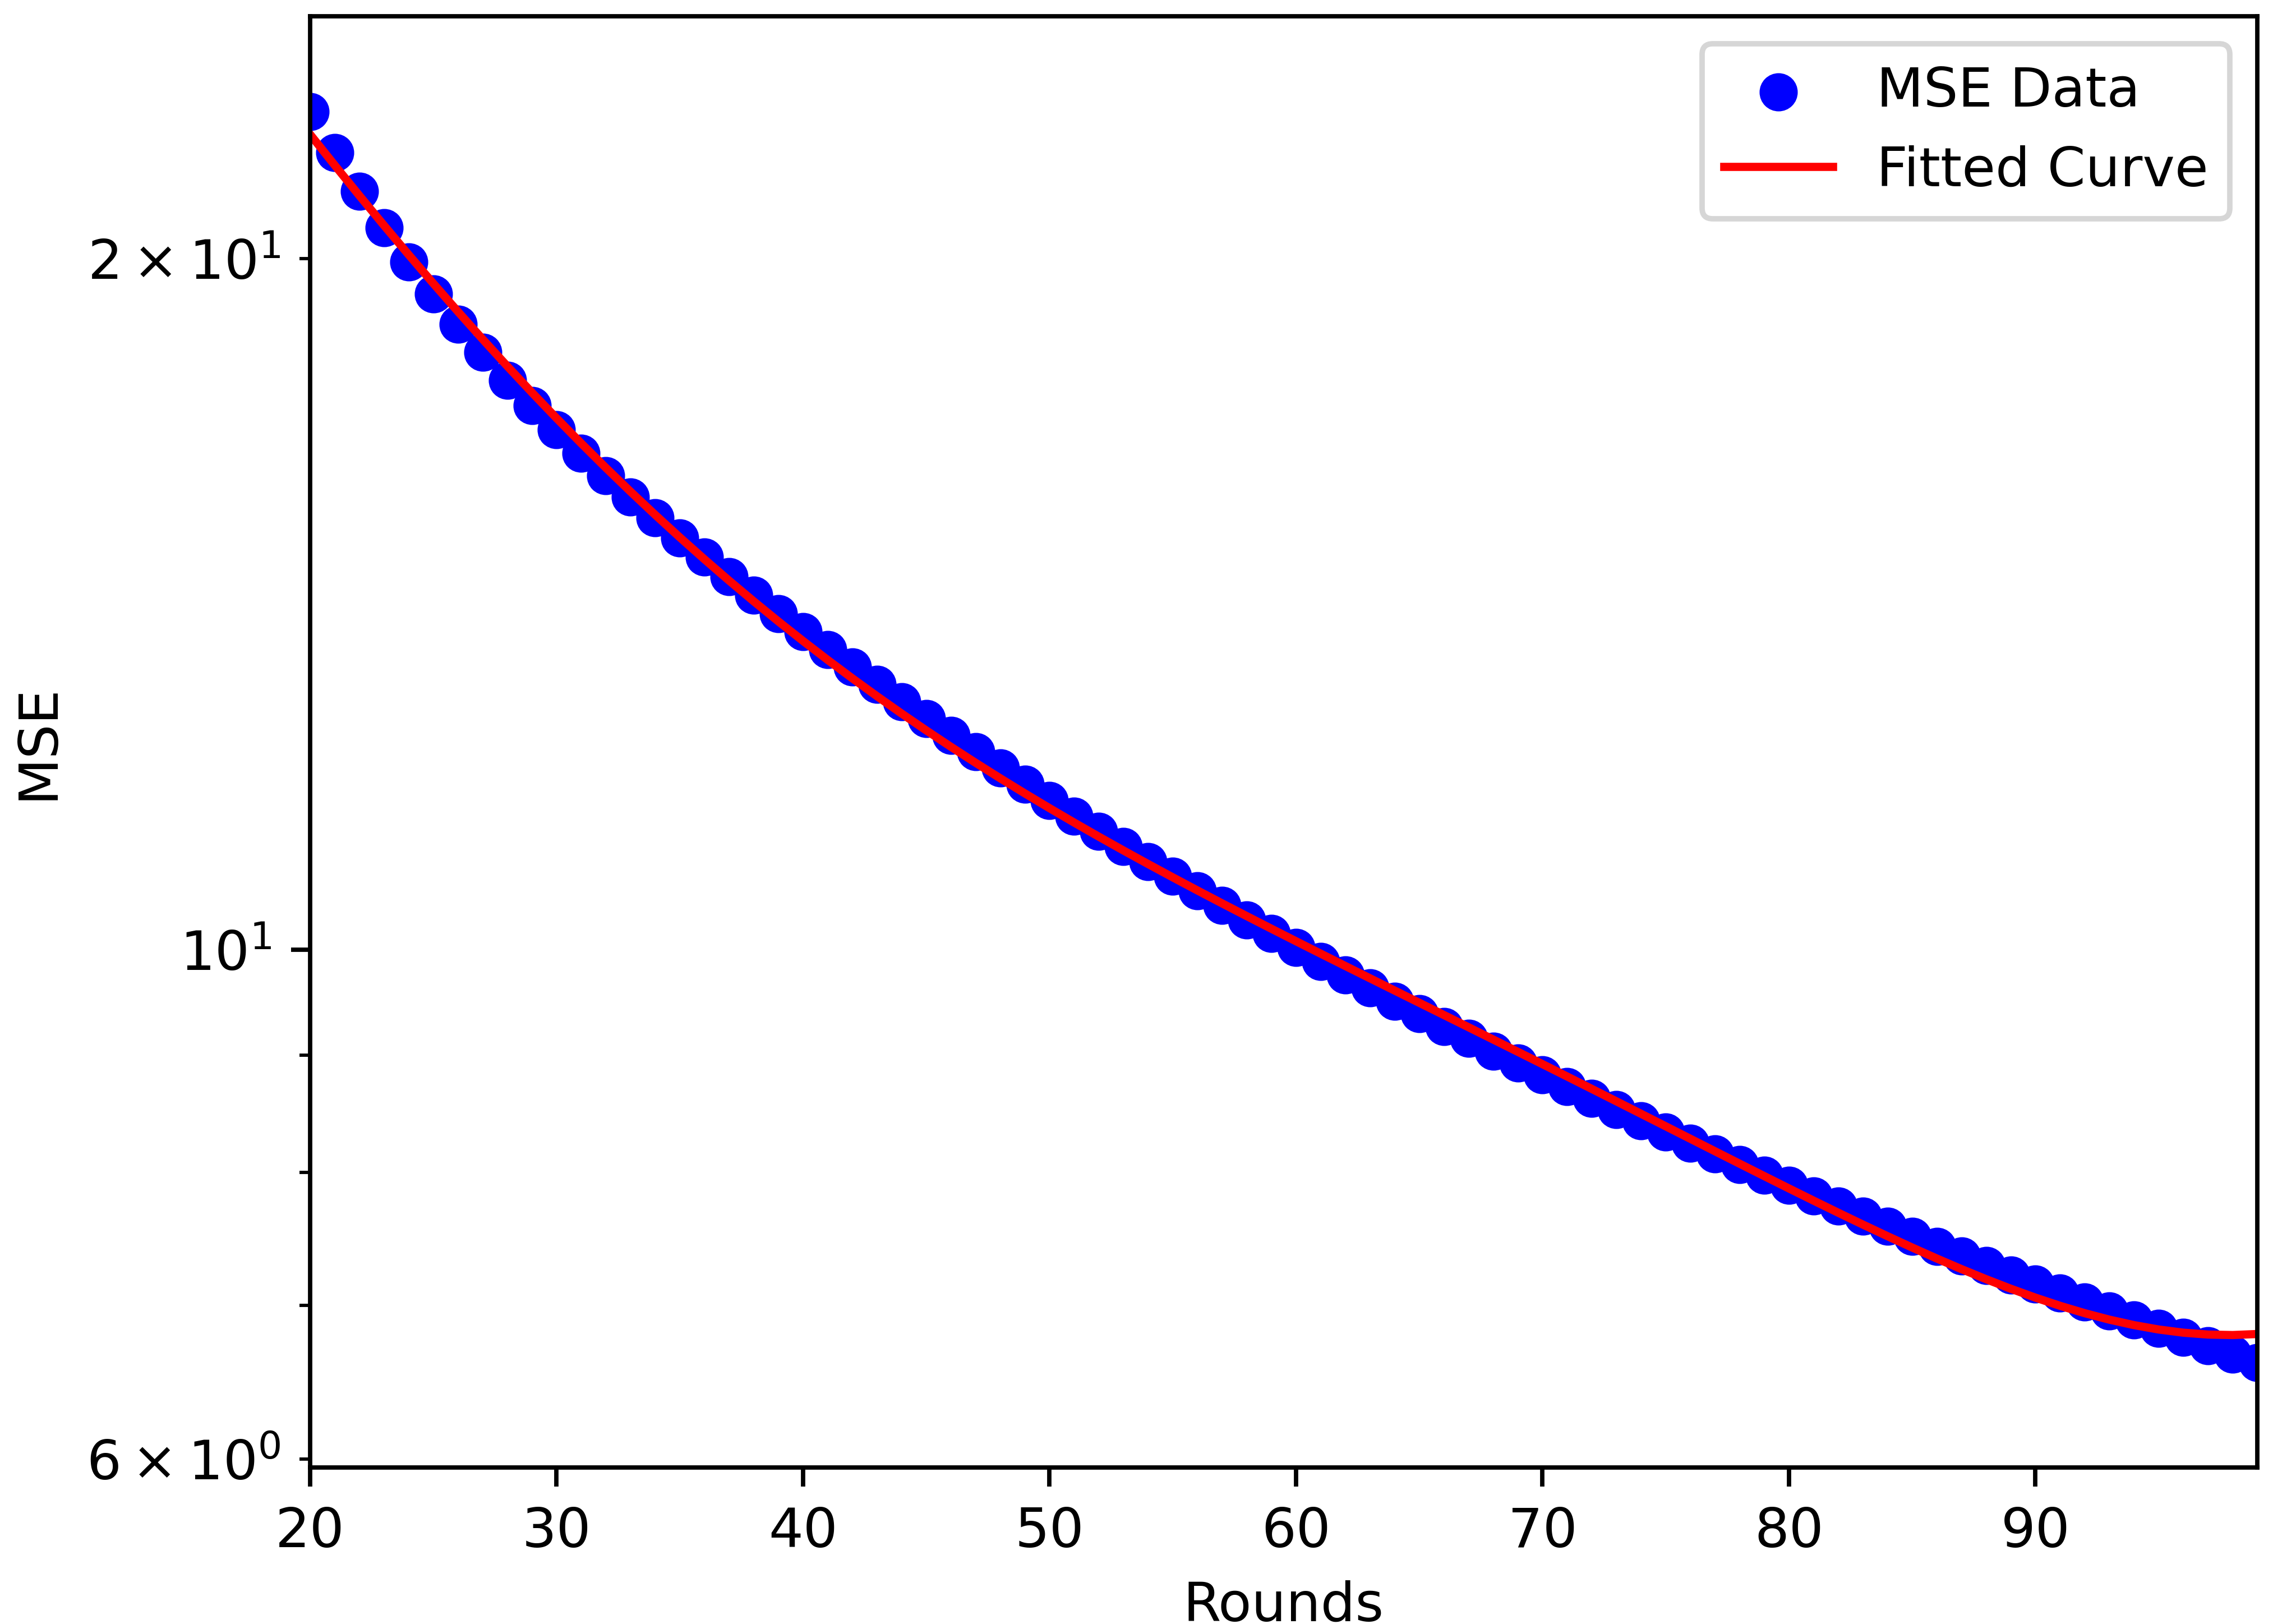
\includegraphics{figures/Simulation_outcomes/RingOfCliques/32x32/DAB/DAB_modelfitting_rounds_99_model_2.png}}
     \caption{$(32\times32)$-Ring of Cliques - polynomial regression fit: DAB}
     \label{fig:dabRingOfCliquesModelFit}
 \end{figure}
\begin{figure}[]
    \centering
    \scalebox{0.8}{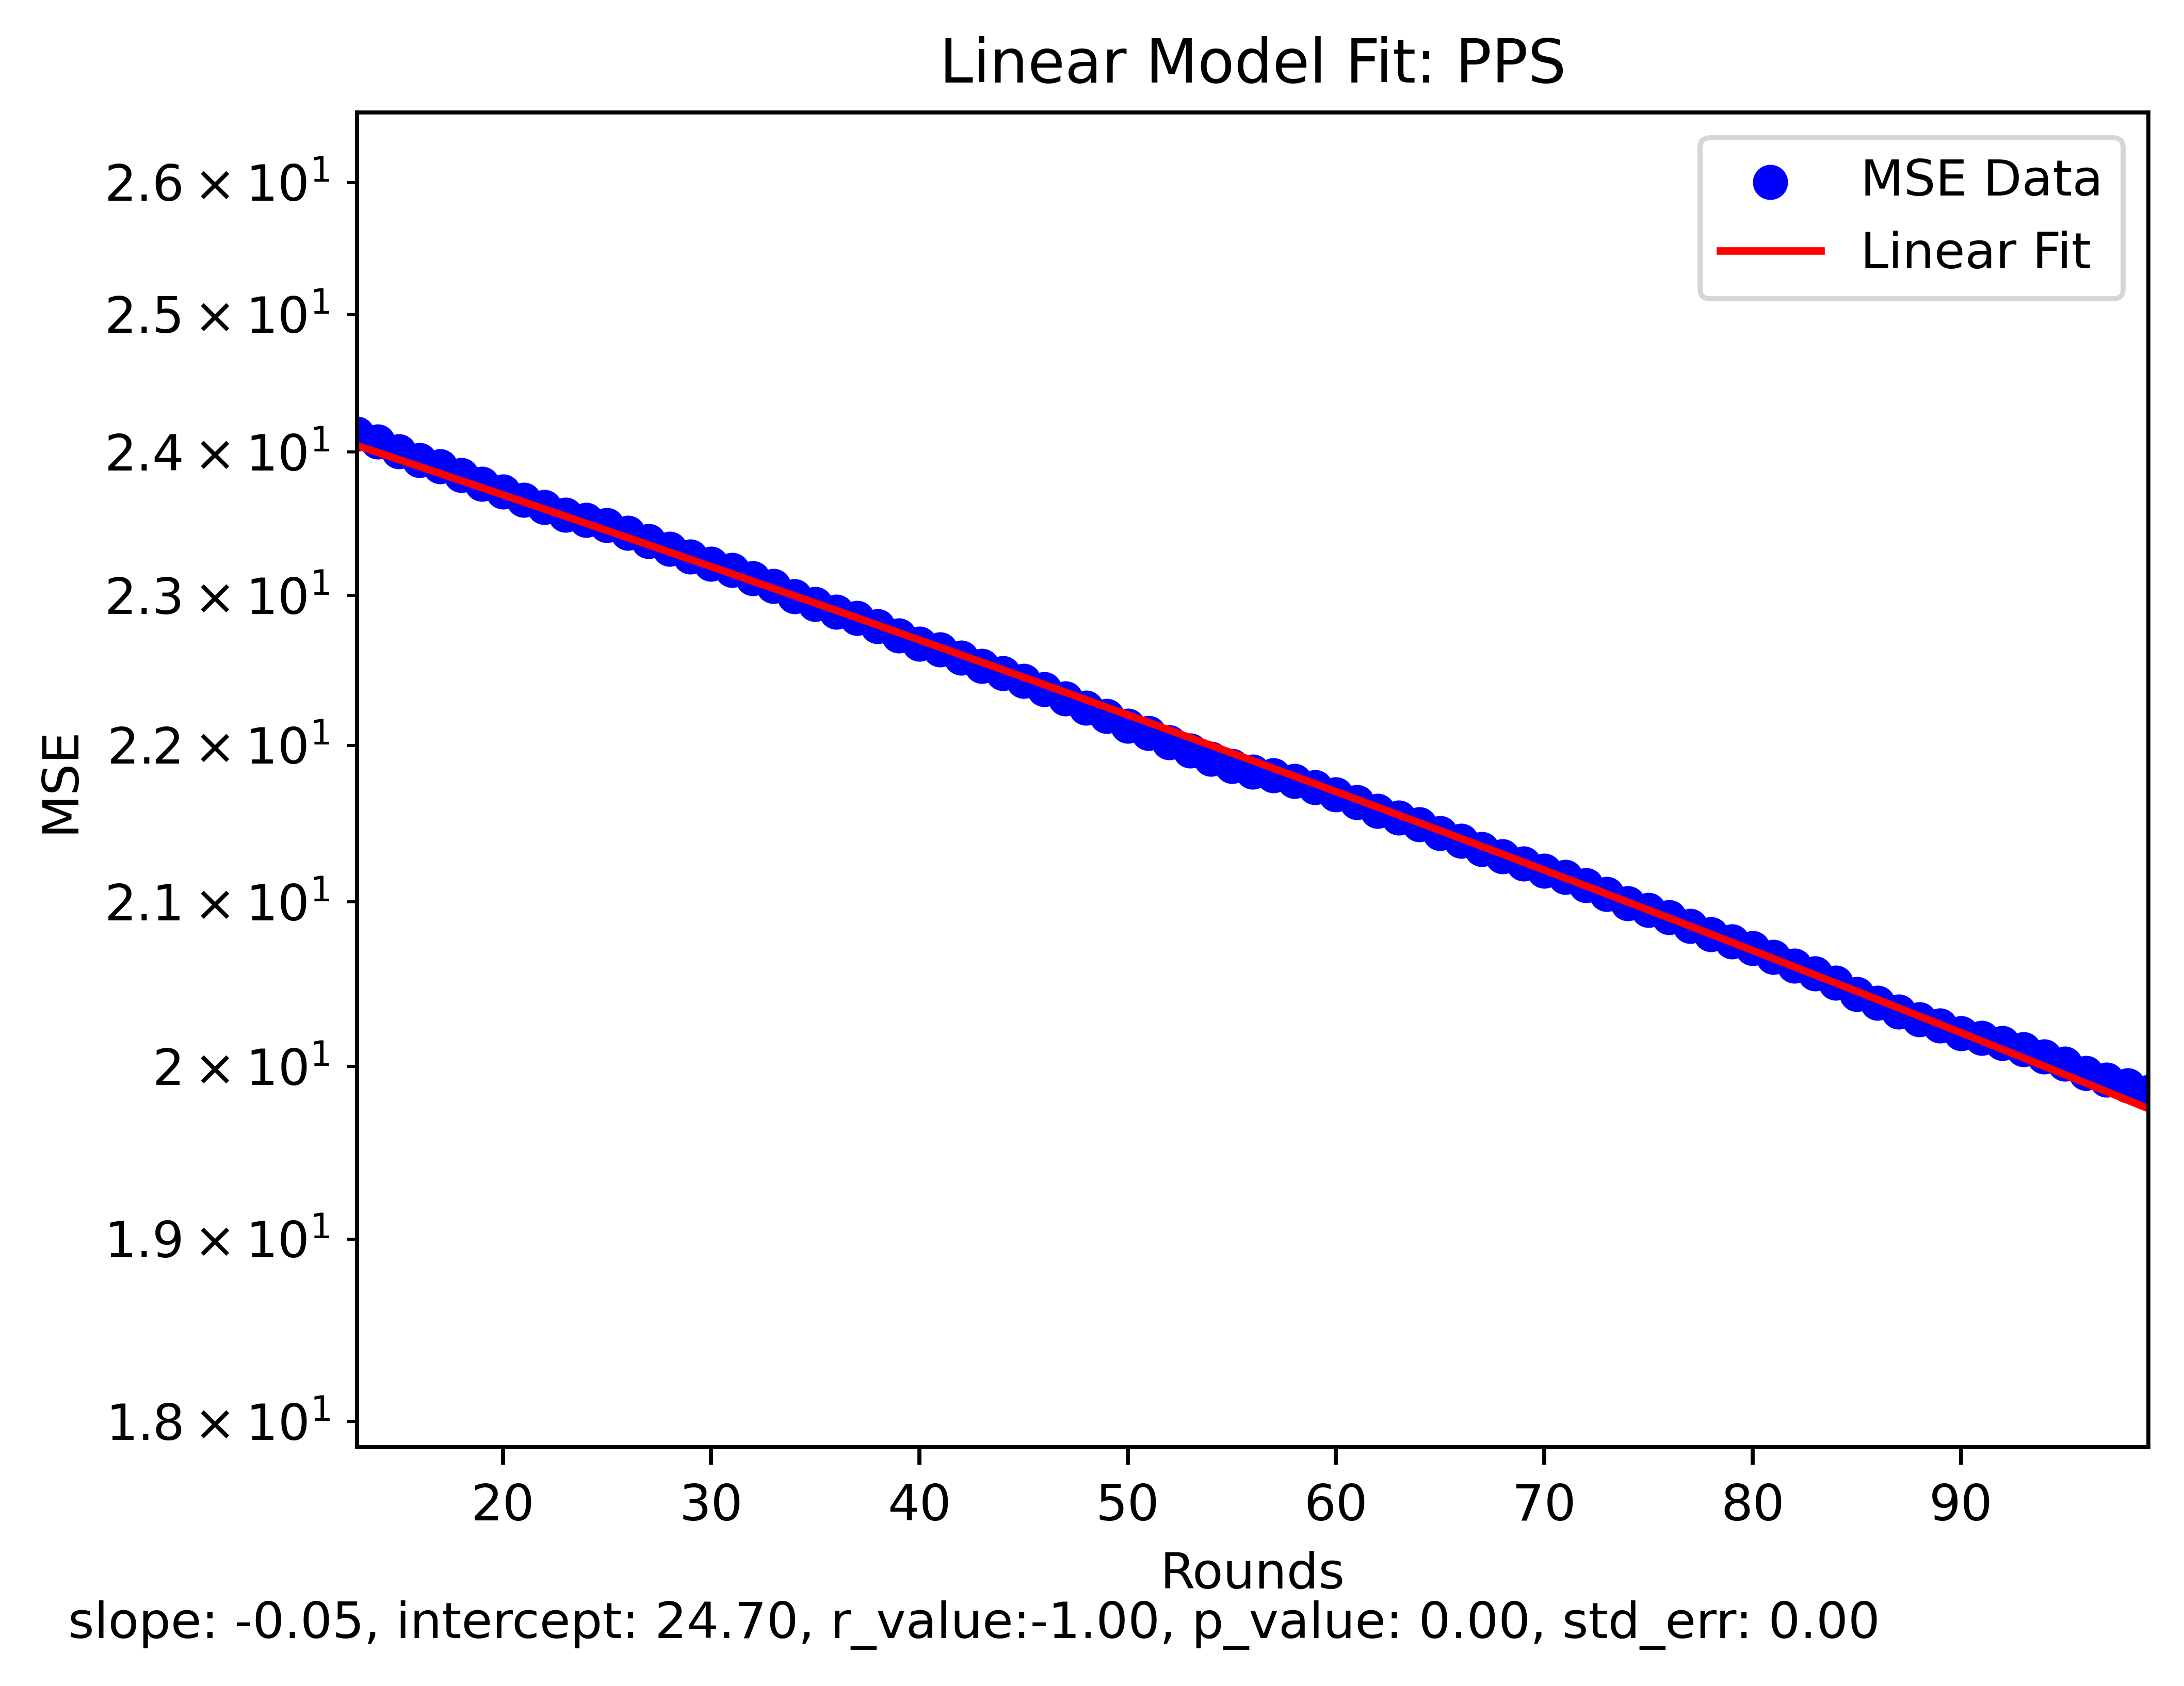
\includegraphics{figures/Simulation_outcomes/RingOfCliques/32x32/PPS/PPS_modelfitting_rounds_99_model_0.png}}
    \caption{$(32\times32)$-Ring of Cliques - polynomial regression fit: PPS}
    \label{fig:ppsRingOfCliquesModelFit}
\end{figure}

\begin{figure}[]
    \centering
    \scalebox{0.8}{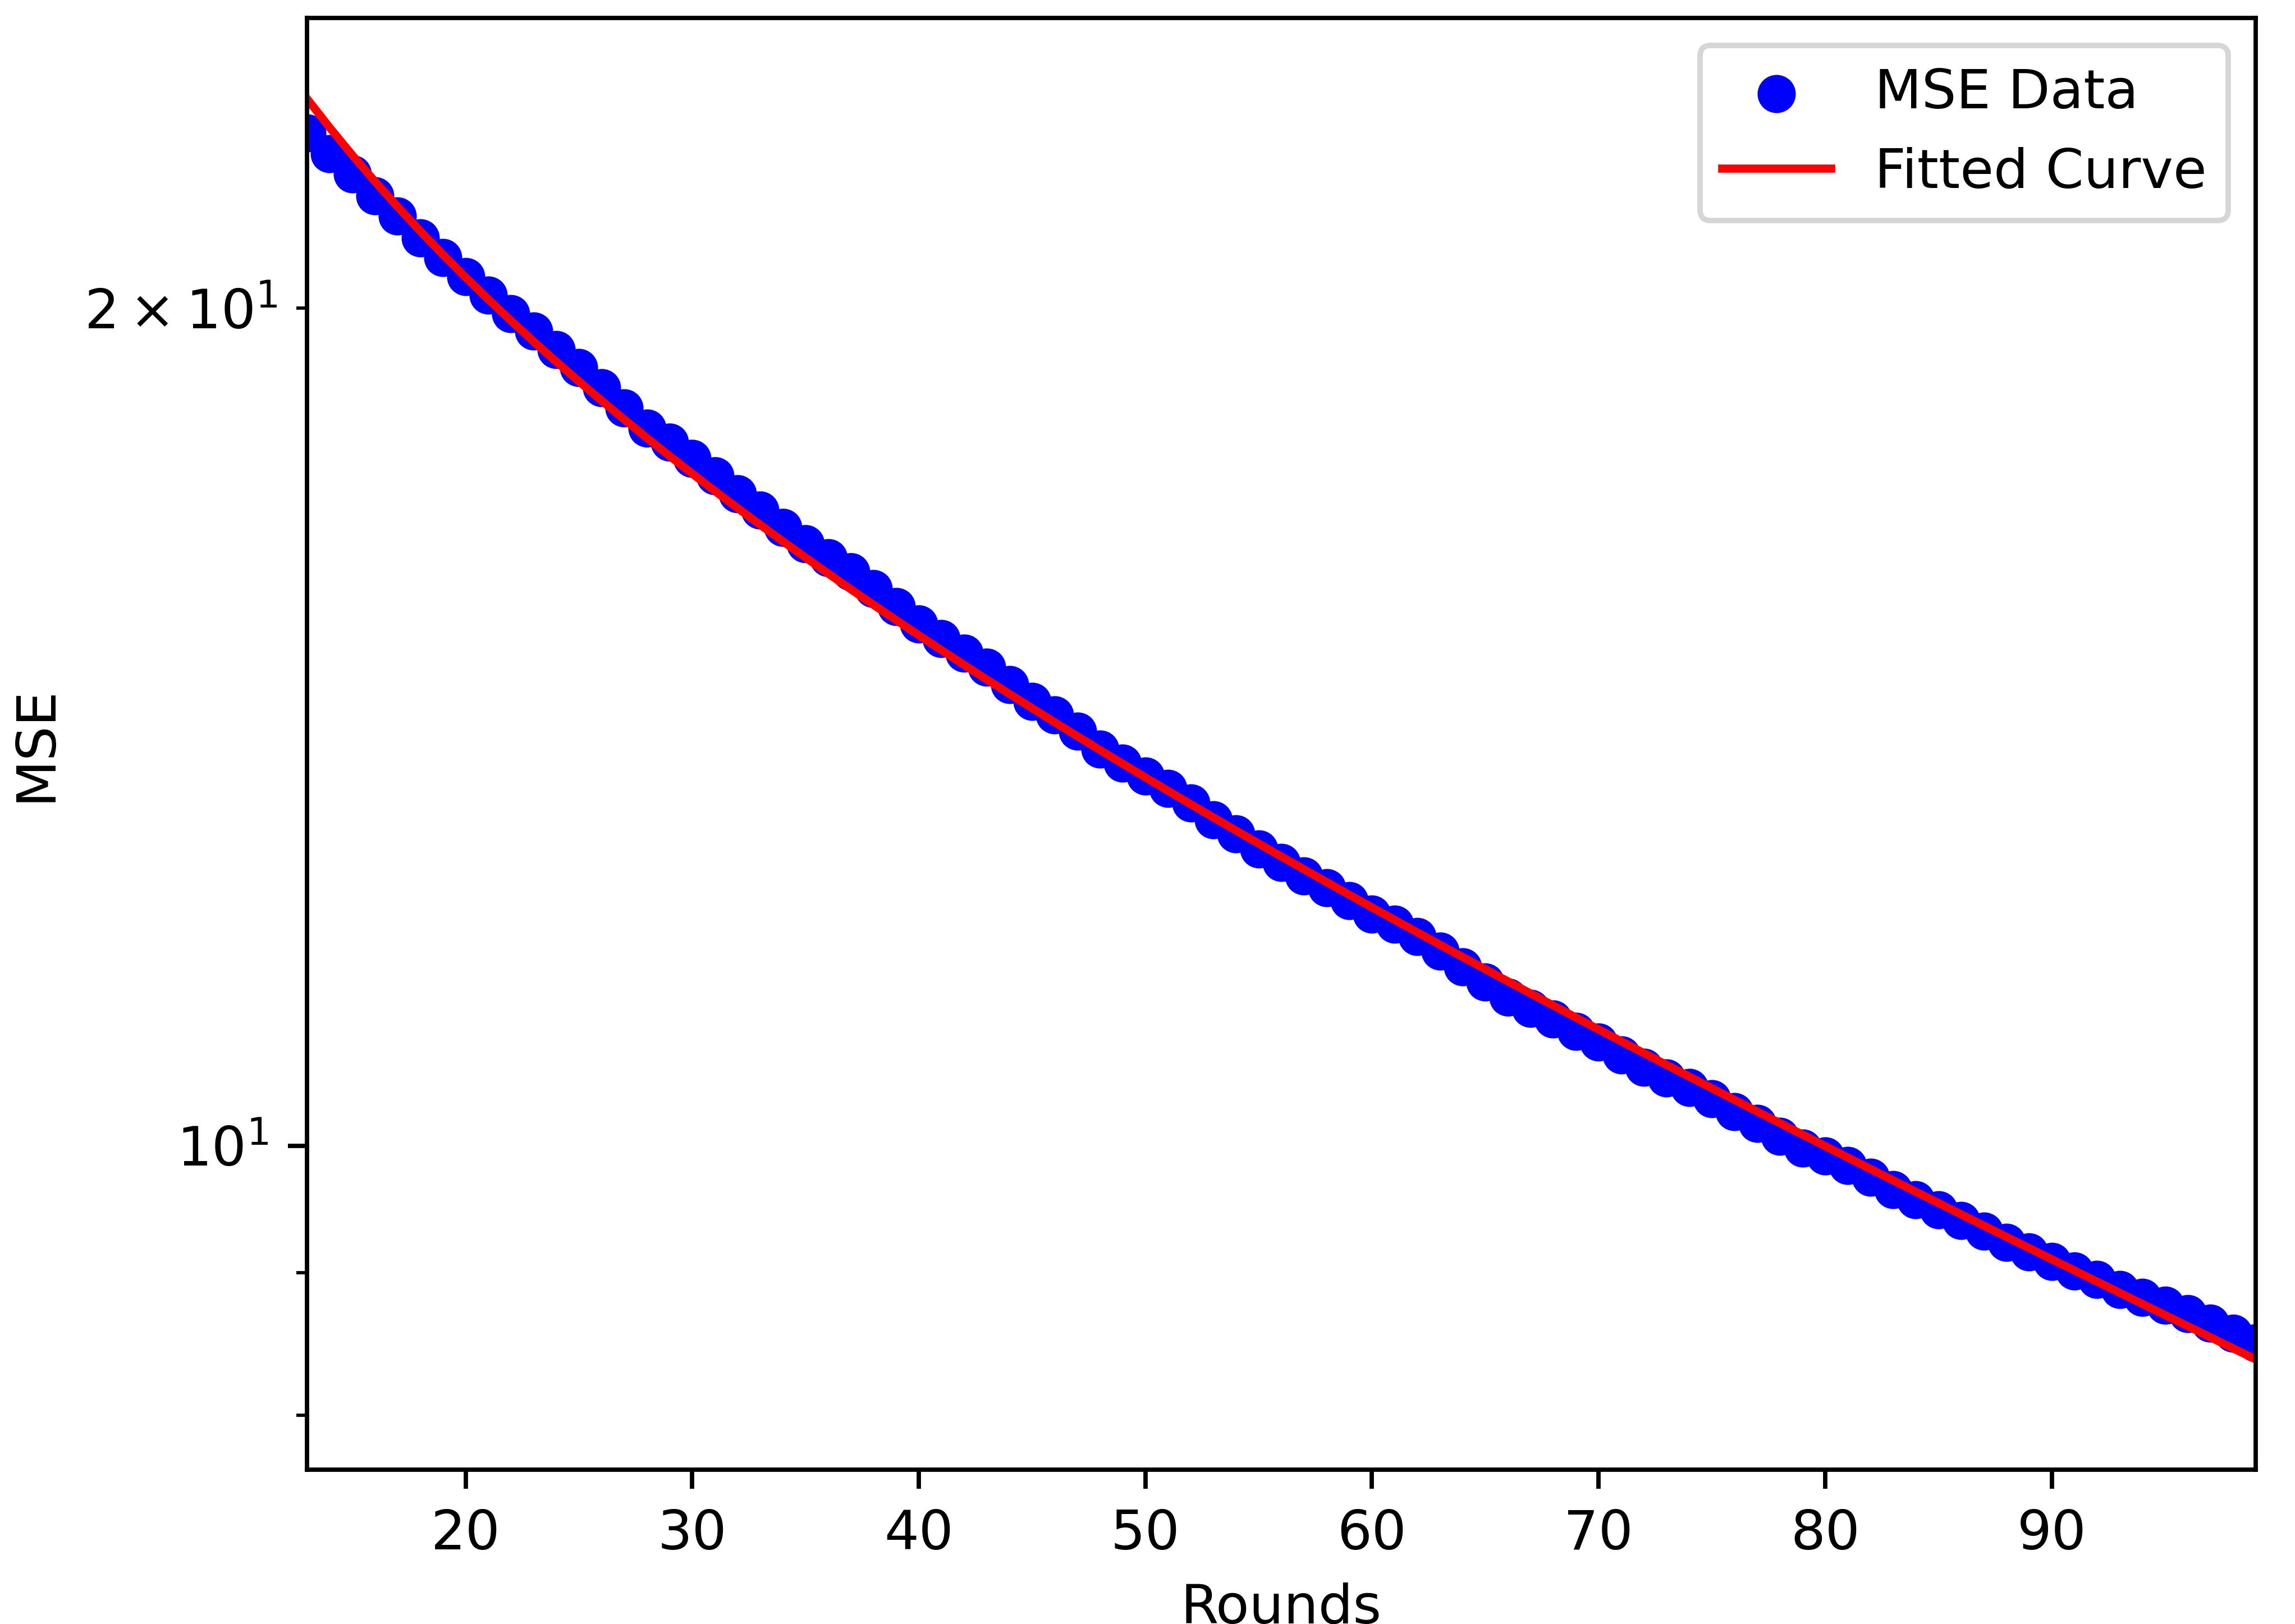
\includegraphics{figures/Simulation_outcomes/RingOfCliques/32x32/ATPPS/ATPPS_modelfitting_rounds_99_model_3.png}}
    \caption{$(32\times32)$-Ring of Cliques - logarithmic regression fit: ATPPS}
    \label{fig:atppsRingOfCliquesModelFit}
\end{figure}

\begin{figure}
    \centering
    \scalebox{0.8}{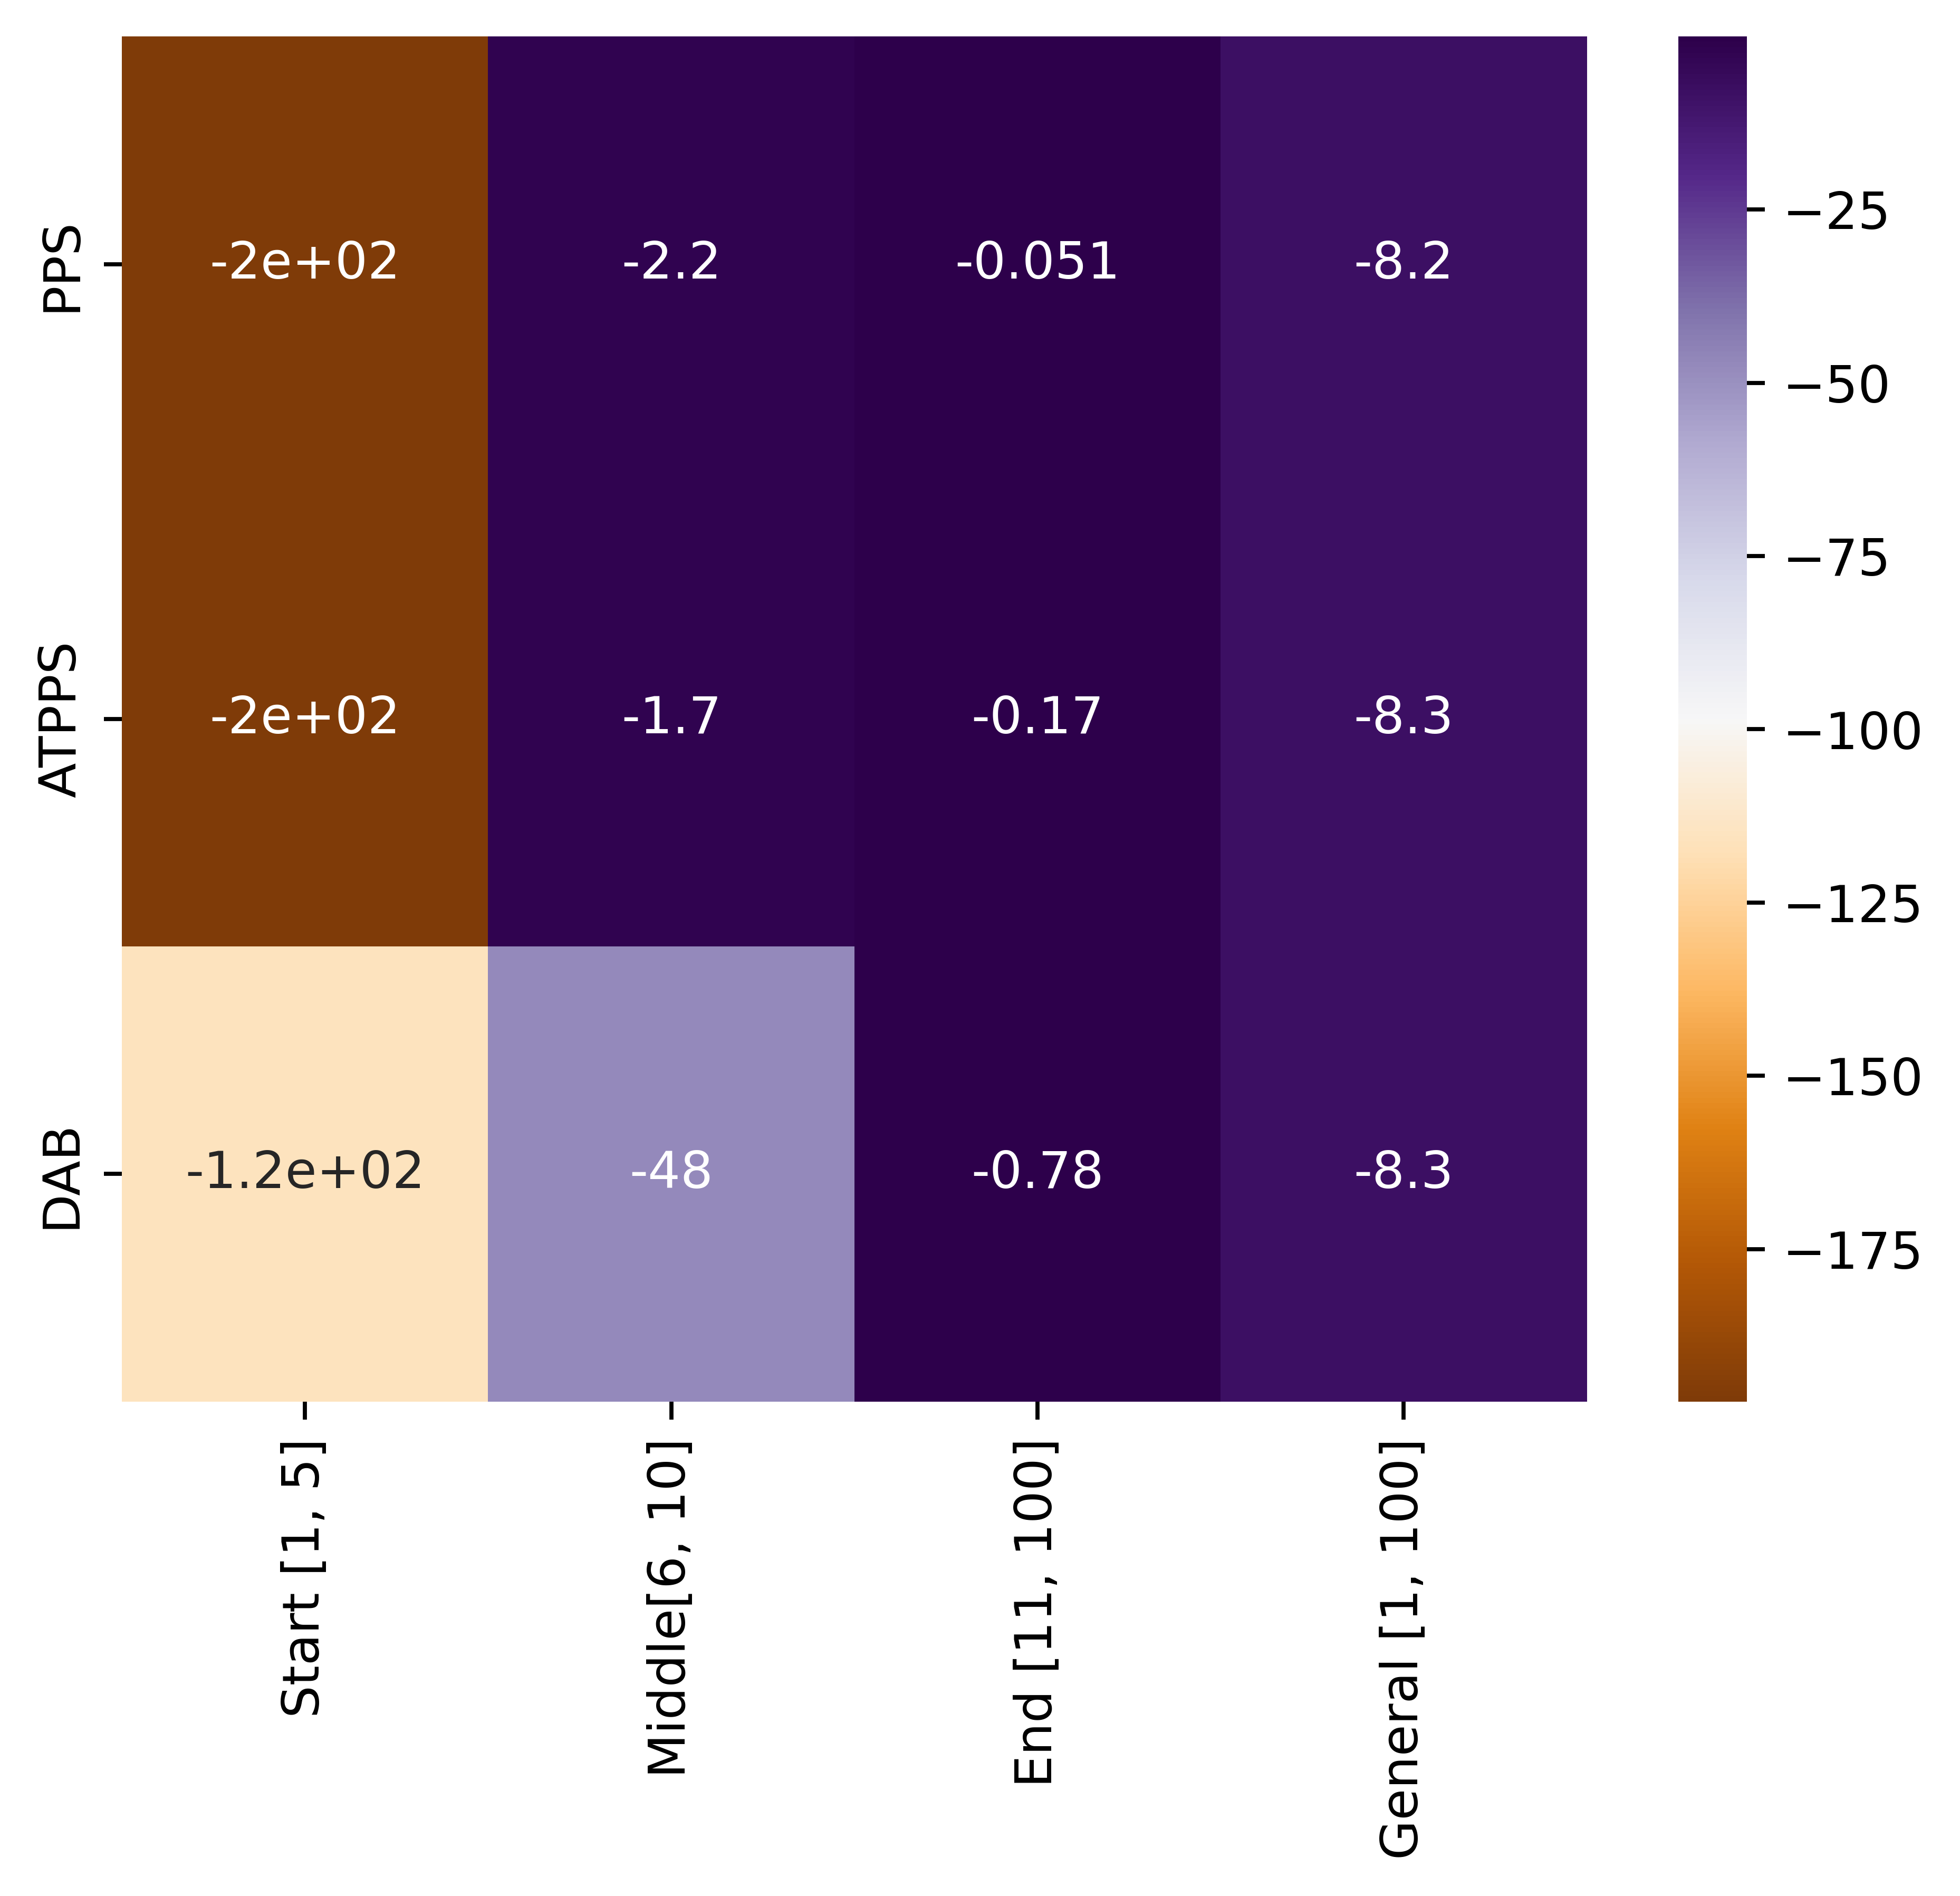
\includegraphics{figures/Simulation_outcomes/RingOfCliques/32x32/DAB_vs_PPS_vs_ATPPS_slopesheatmap_100rounds.png}}
    \caption{$(32\times32)$-Ring of Cliques: heat map of slopes per region}
    \label{fig:ringOfCliquesslopes}
\end{figure}

In the following the Ring of Cliques are newly organized. Experiments are conducted where the number of cliques is increased from $2^{5}$ to $2^{7}$ in subsection \ref{subsec:128_8ROC} and thus the clique size of each clique is decreased to $2^{3}$. Subsection \ref{subsec:8_128ROC} covers the experiment where the clique size is increased and the number of cliques is decreased in the same magnitude as discussed before.

\subsection{128x8 Ring of Cliques}\label{subsec:128_8ROC}
The clique size plays a crucial role for the efficacy of the DAB algorithm. The decreased clique size favors the DAB making it the load balancing algorithm to reduce the error in the network more rapidly than the Push-Pull Sum based algorithms as seen in figure \ref{fig:128x8RingOfCliquesLog_LogLog}. All the load balancing algorithms show an rapid decrease of error in the network, indicated by the steep negative slopes as visualized in figure \ref{fig:128x8ringOfCliquesslopes}. The Push-Pull Sum based algorithms show an decrease of -180, whereas the DAB shows a decrease of -190 in the start region (rounds 1 to 5). After the very steep decrease in the start region the load balancing algorithms decrease the error more moderately, where the DAB algorithm still has the steepest decrease of error of -5.2, followed by the ATPPS decreasing the error as low as -4.6, lastly the PPS follows with a slope of -3.6. The curve in this region is rather flat as seen in the log-log representation in figure \ref{fig:128x8RingOfCliquesLog_LogLog} a) The decrease effect diminishes as the error of the network is already relatively low, in the end region. The MSE values at the end of round of 100 show the magnitude of error reduction. The DAB scored the lowest MSE value 10.64, followed by the ATPPS achieving very good results to with a MSE value of 13.68. The PPS value achieved the highest MSE value of 22.33. Compared to the $(32\times 32)$-Ring of Cliques the load balancing algorithms reduced the error even more by a margin of 2 to 4 units. The most improvement is drawn by the ATPPS with a lower value of around around 5 followed by the DAB, with a lower MSE of 4 and lastly the PPS with a decreased value of around 2.

All three load balancing algorithms were fitted against polynomials with degree 4. The equations are as follows: DAB $MSE_r=5.45\times 10 ^{-7}r^{4}-1.7\times 10^{-4}r^{3}+0.02r^{2}-1.33r+46.71$ (figure \ref{fig:128x8dabRingOfCliquesModelFit}) PPS: $MSE_r=1.04\times 10 ^{-6}r^{4}-3.41\times 10^{-4}r^{3}+0.04r^{2}-2.73r+97.58$ (figure \ref{fig:128x8ppsRingOfCliquesModelFit}) and ATPPS: $MSE_r=9.54\times 10^{-7}r^{4}-2.93\times 10^{-4}r^{3}+0.03r^{2}-2.05r+67.02$ (figure \ref{fig:128x8atppsRingOfCliquesModelFit}).
\begin{figure}[!ht]
    \centering
        \subfloat[]{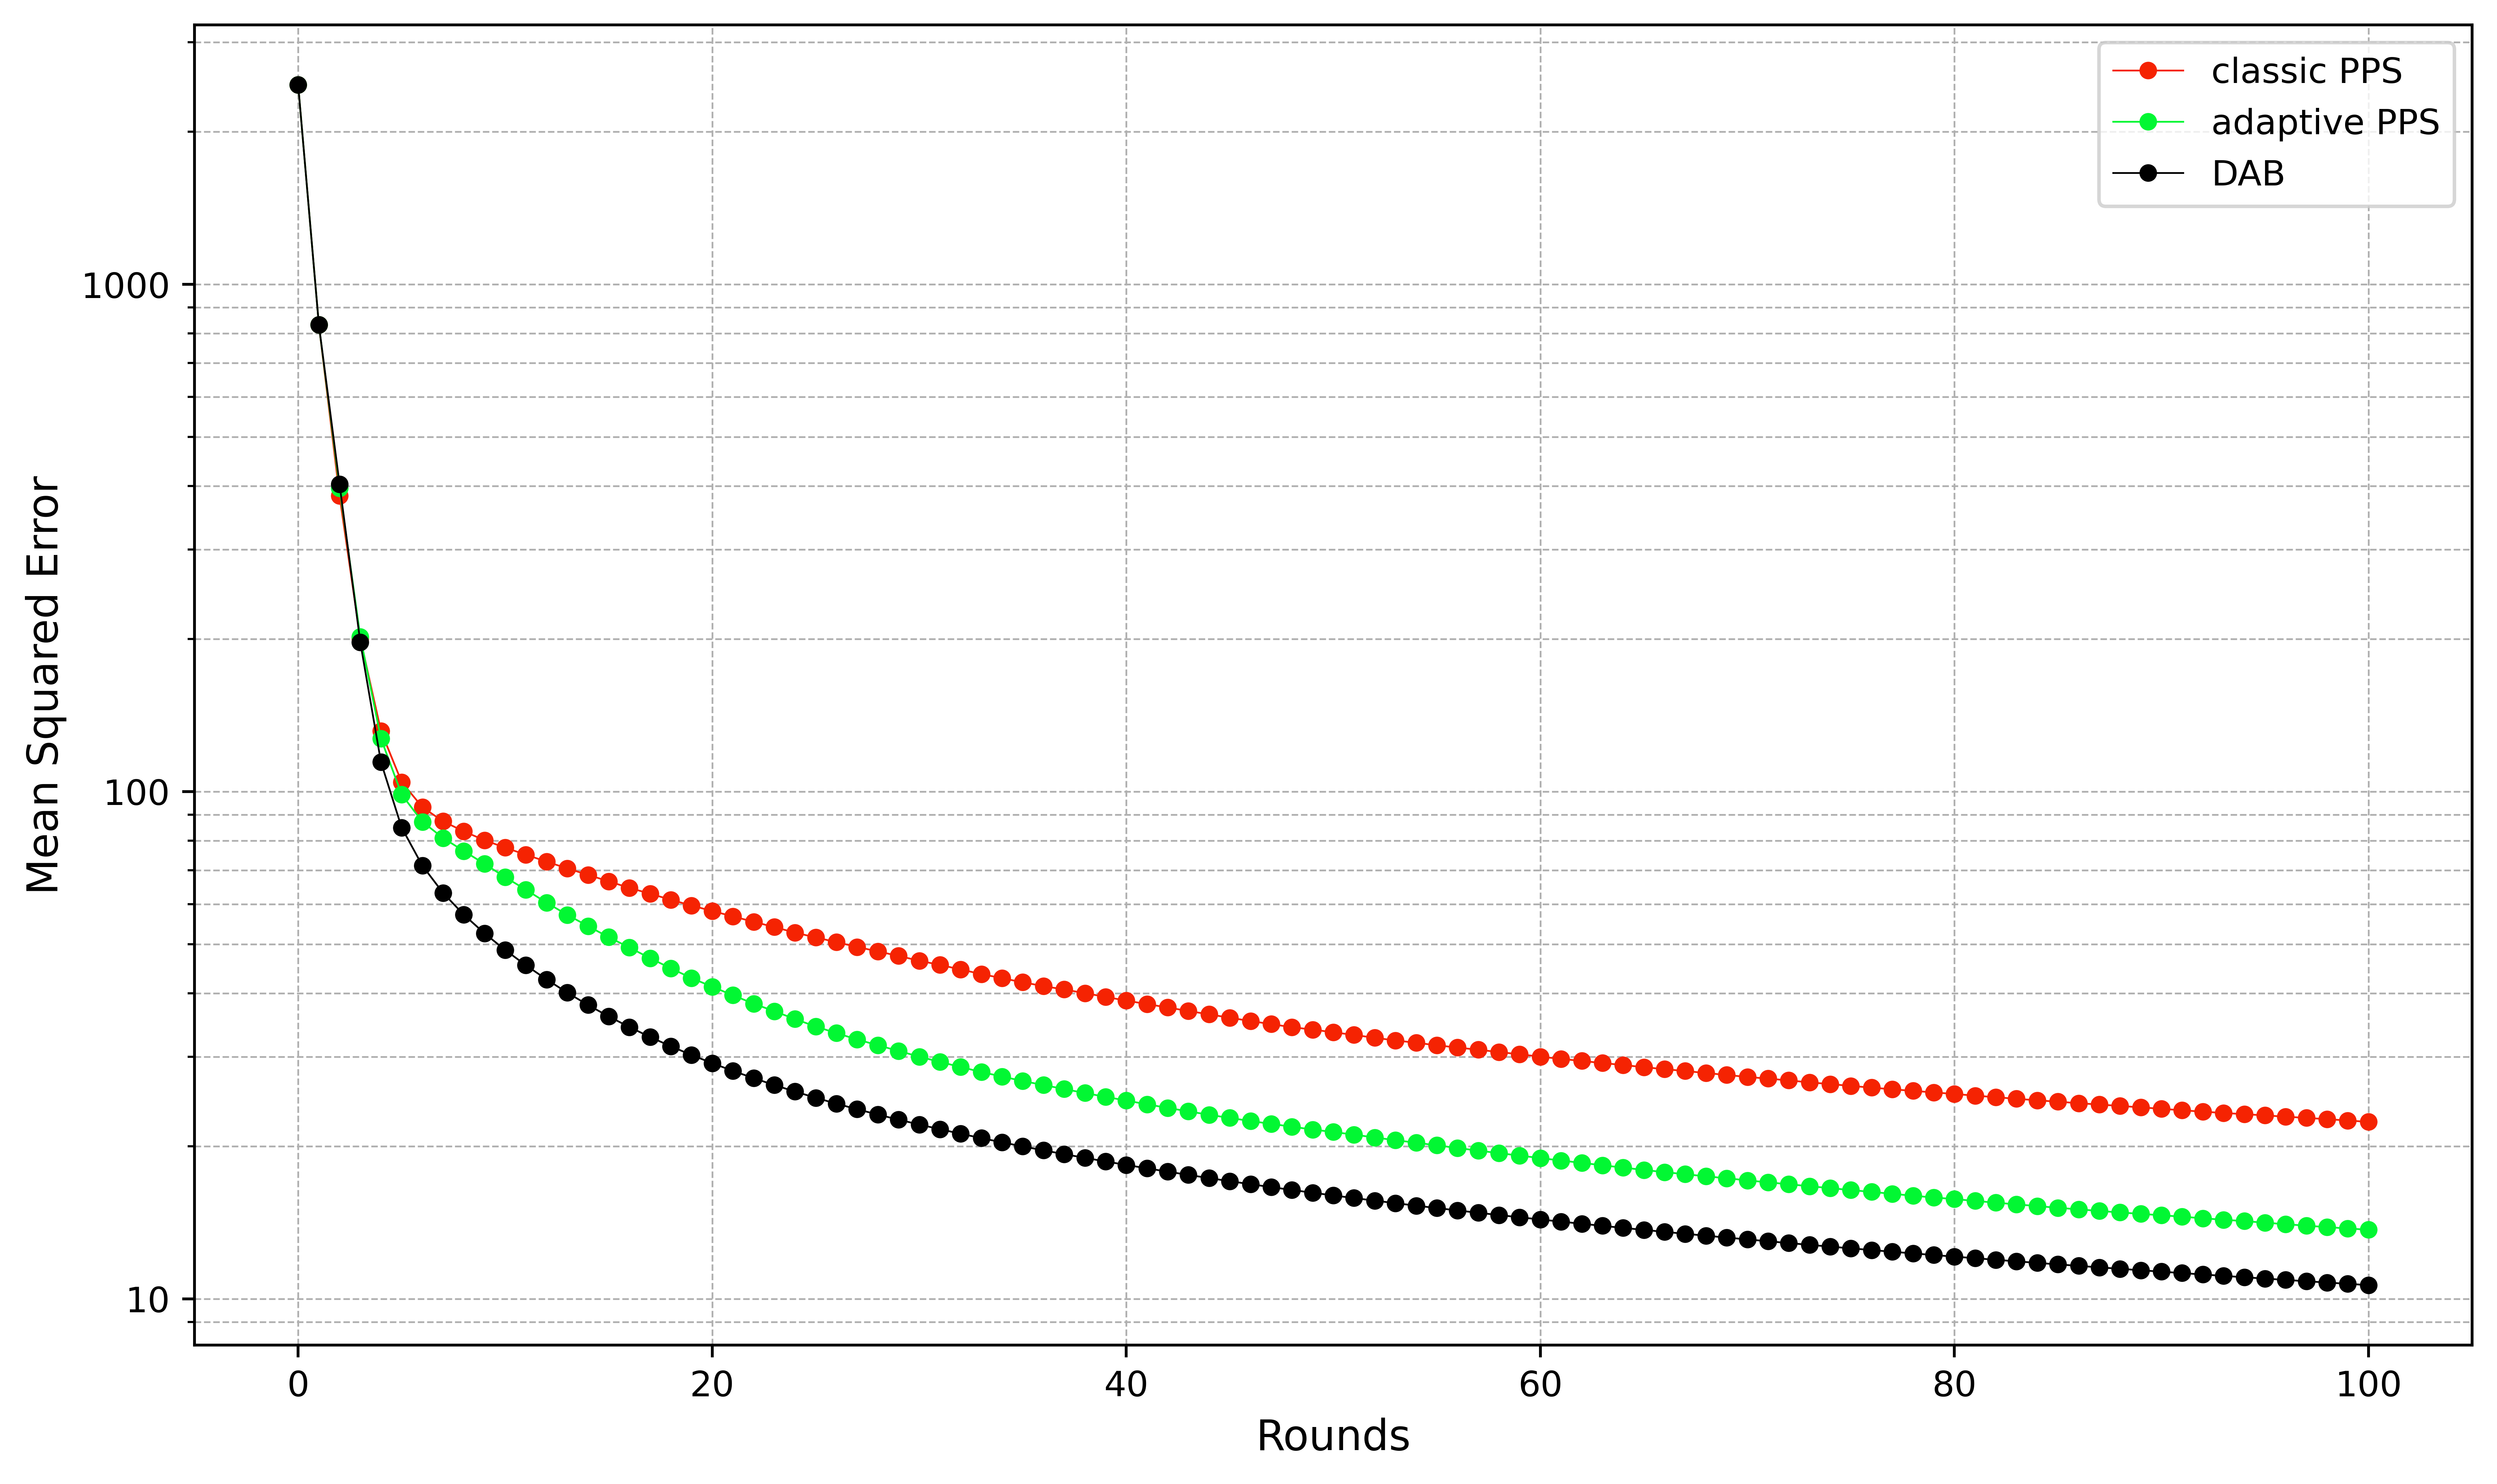
\includegraphics[width=0.49\linewidth]{figures/Simulation_outcomes/RingOfCliques/128x8/DAB_vs_PPS_RoC_r100_n1024_averaged_log.png}}
    \hfil
        \subfloat[]{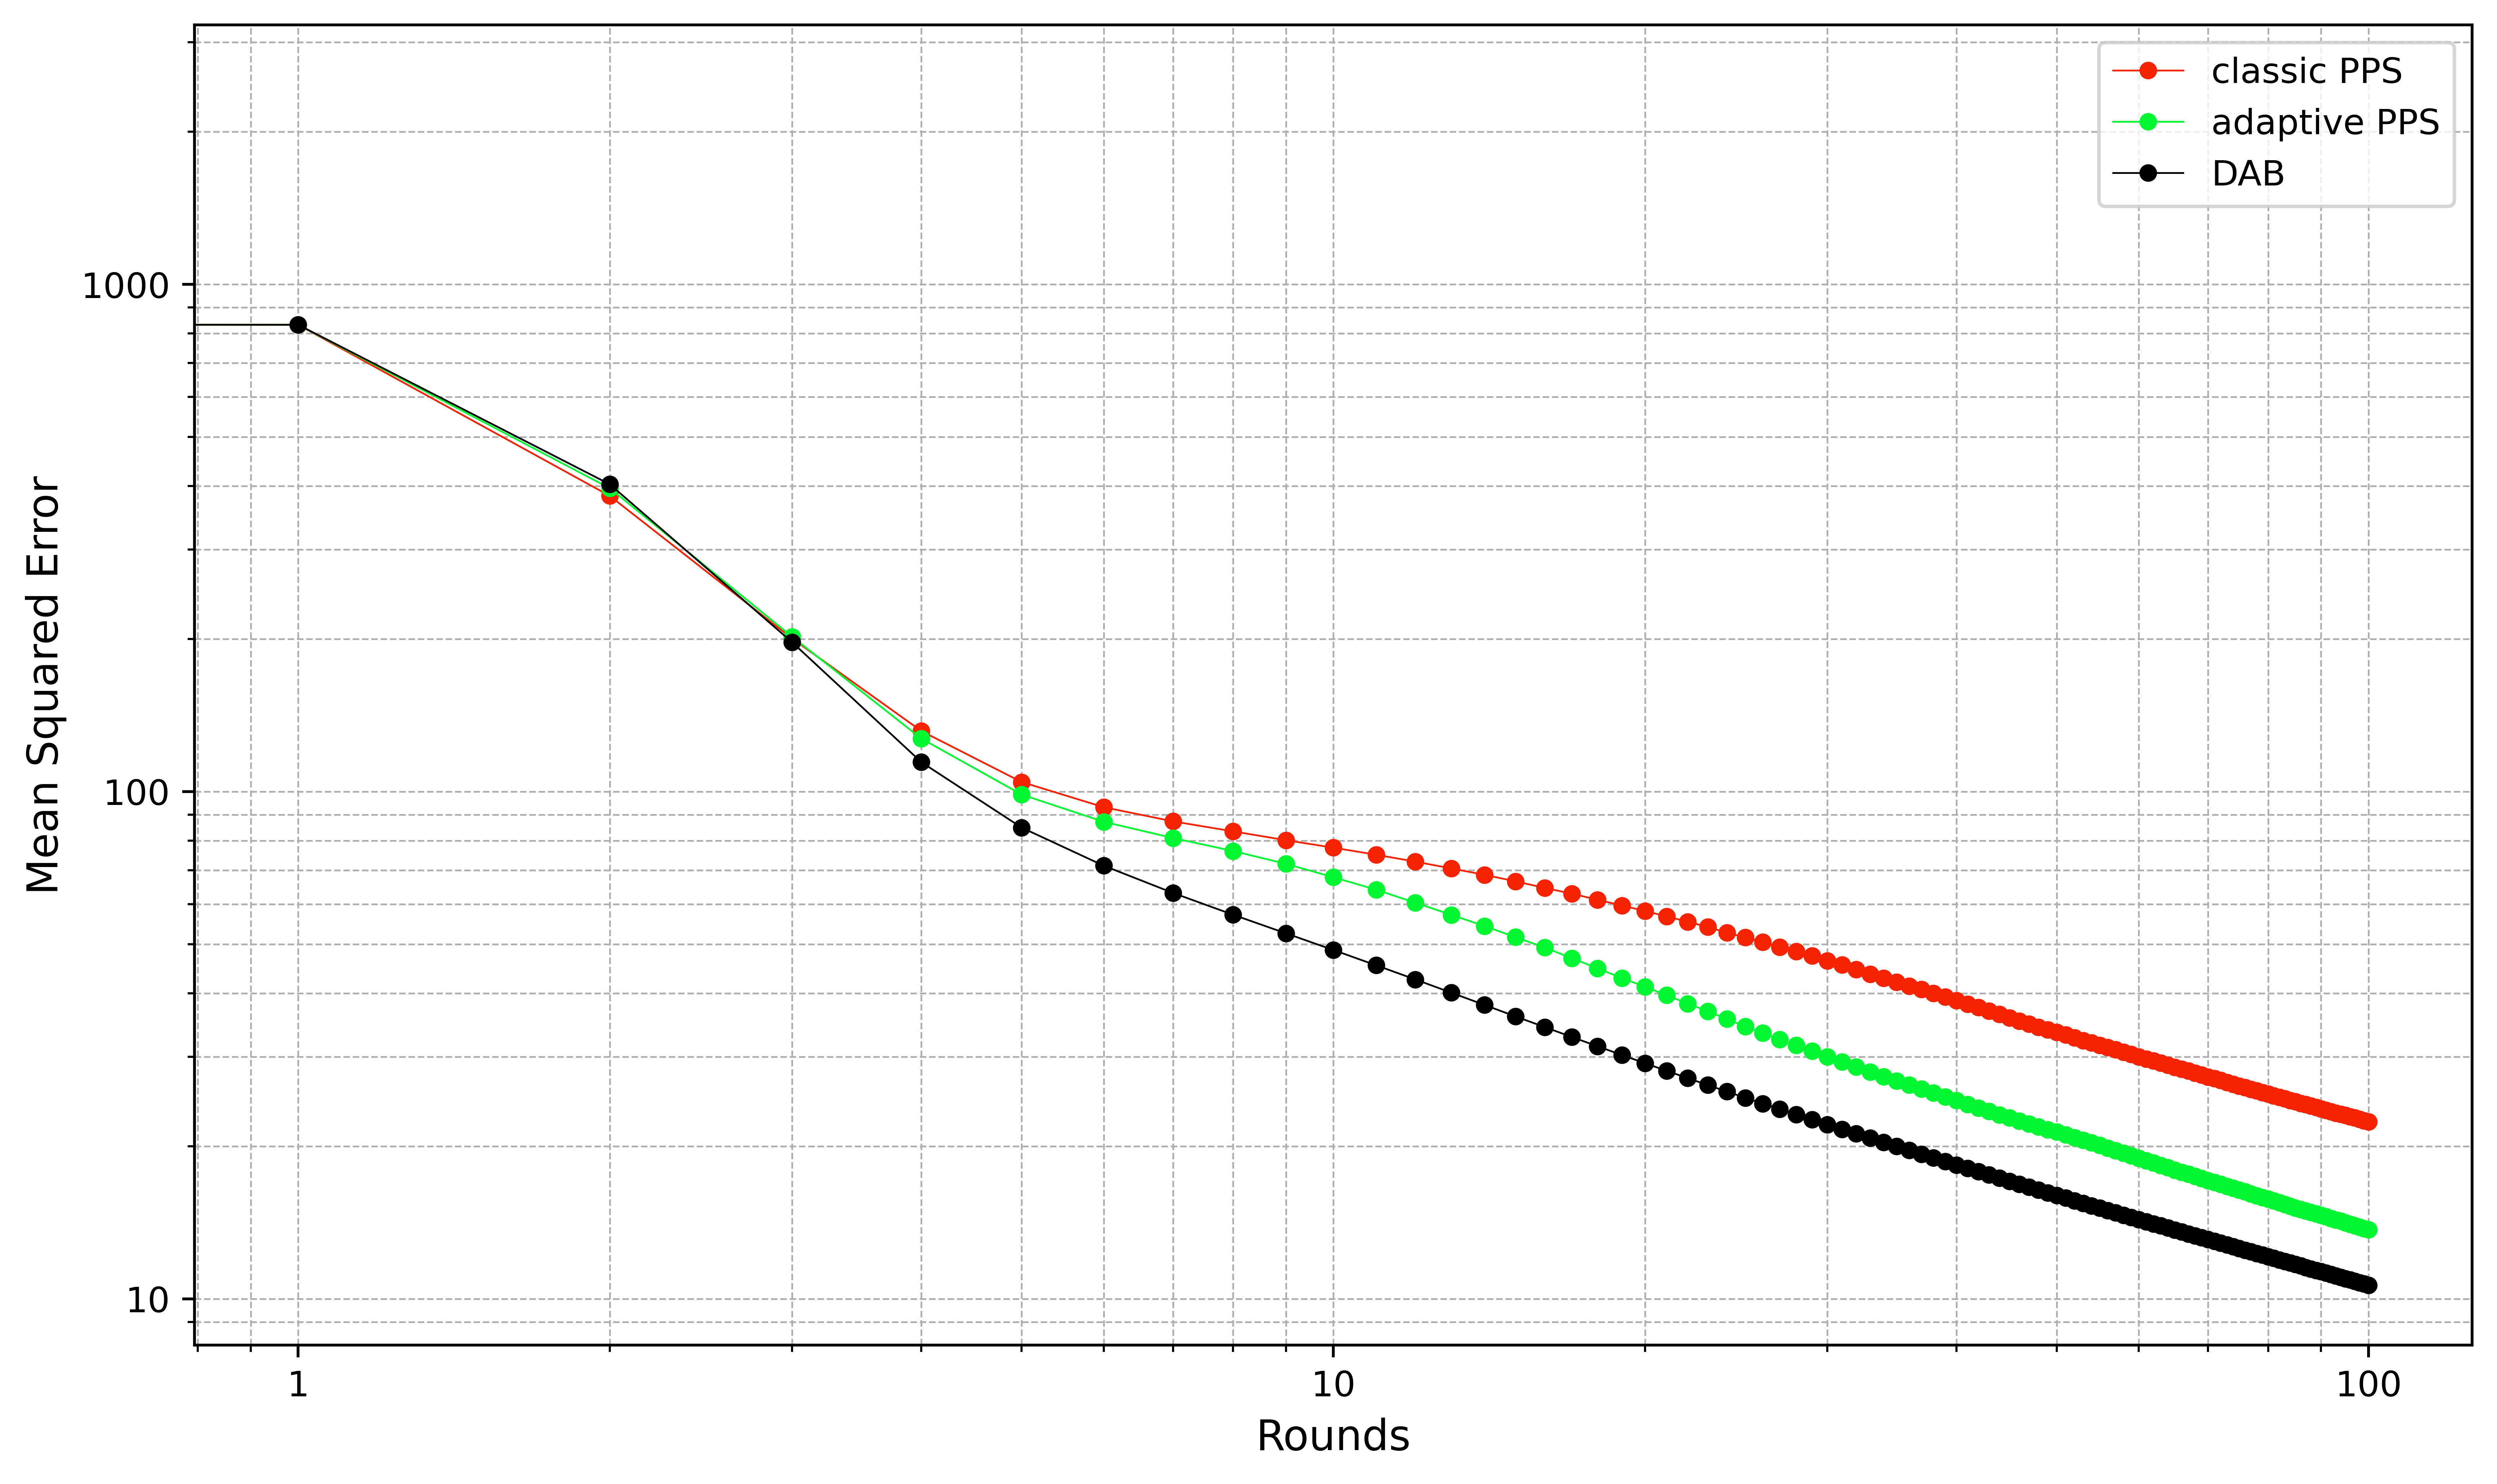
\includegraphics[width=0.49\linewidth]{figures/Simulation_outcomes/RingOfCliques/128x8/DAB_vs_PPS_RoC_r100_n1024_averaged_loglog.png}}
    \caption{$(128\times8)$-Ring of Cliques: mean squared error per rounds (log-linear and log-log)}
        \label{fig:128x8RingOfCliquesLog_LogLog}
\end{figure}

\begin{figure}[]
     \centering
     \scalebox{0.8}{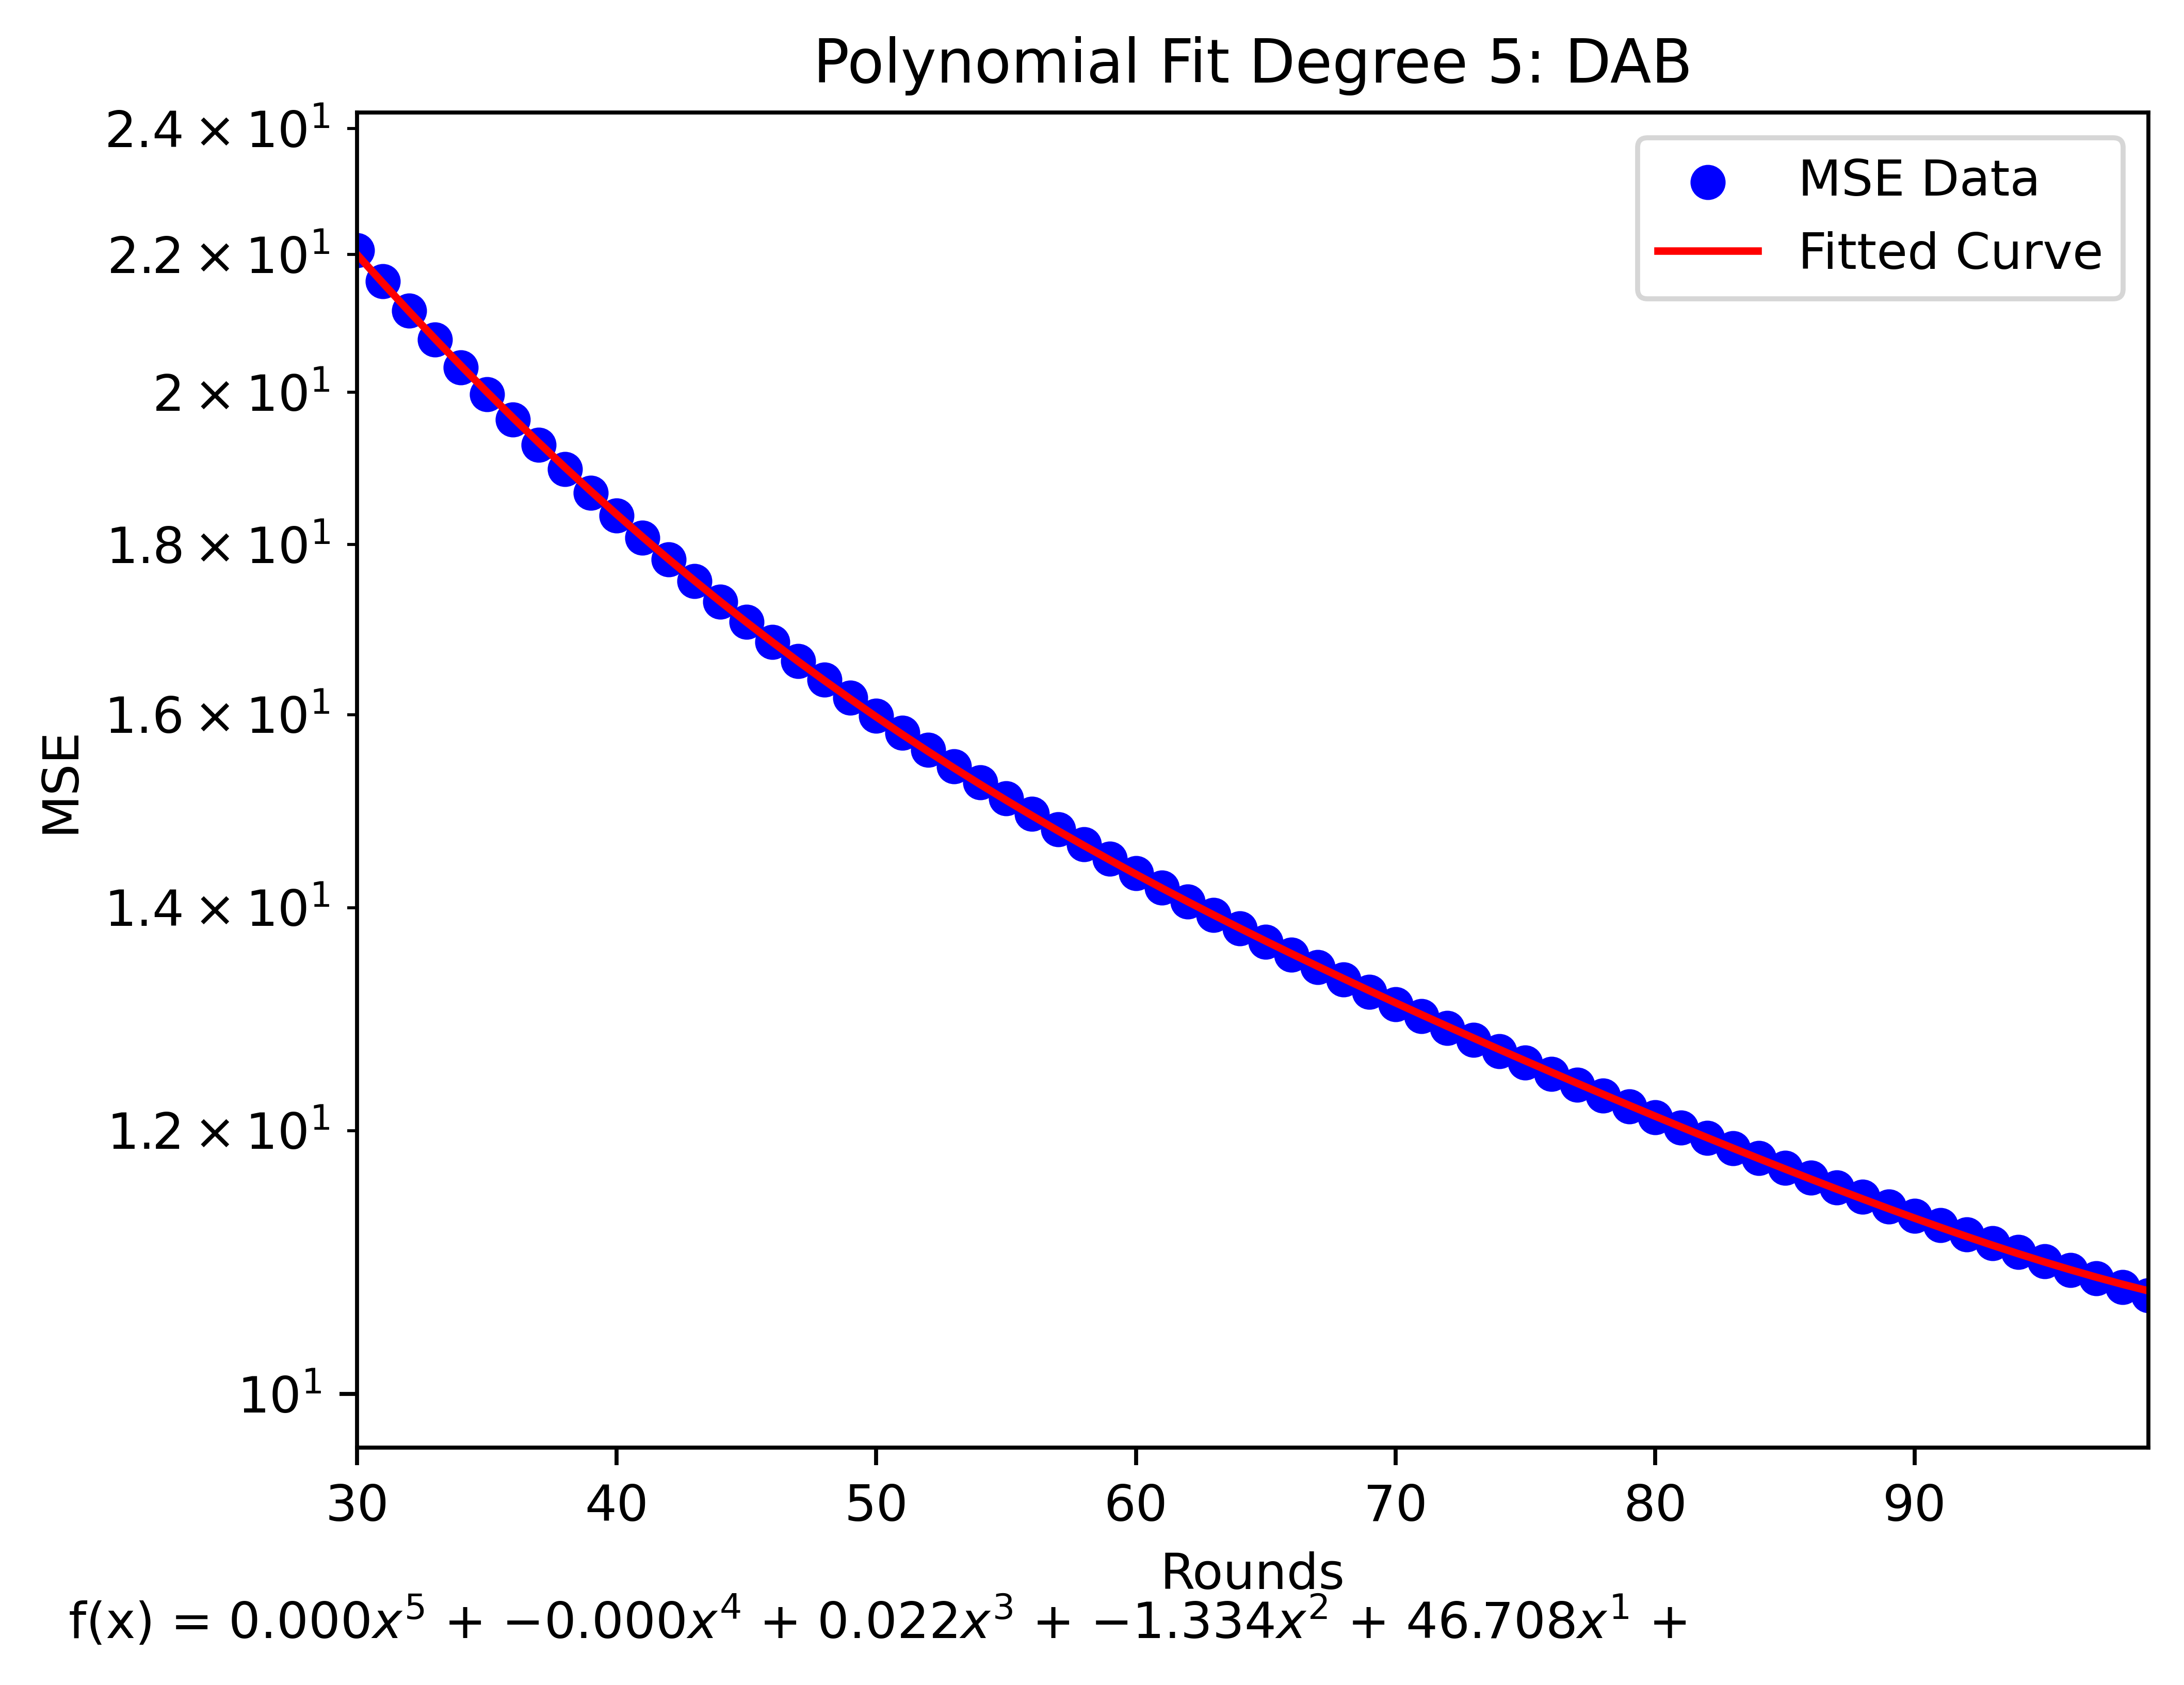
\includegraphics{figures/Simulation_outcomes/RingOfCliques/128x8/DAB/DAB_modelfitting_rounds_99_model_2.png}}
     \caption{$(128\times8)$-Ring of Cliques - polynomial regression fit: DAB}
     \label{fig:128x8dabRingOfCliquesModelFit}
\end{figure}
\begin{figure}[]
    \centering
    \scalebox{0.8}{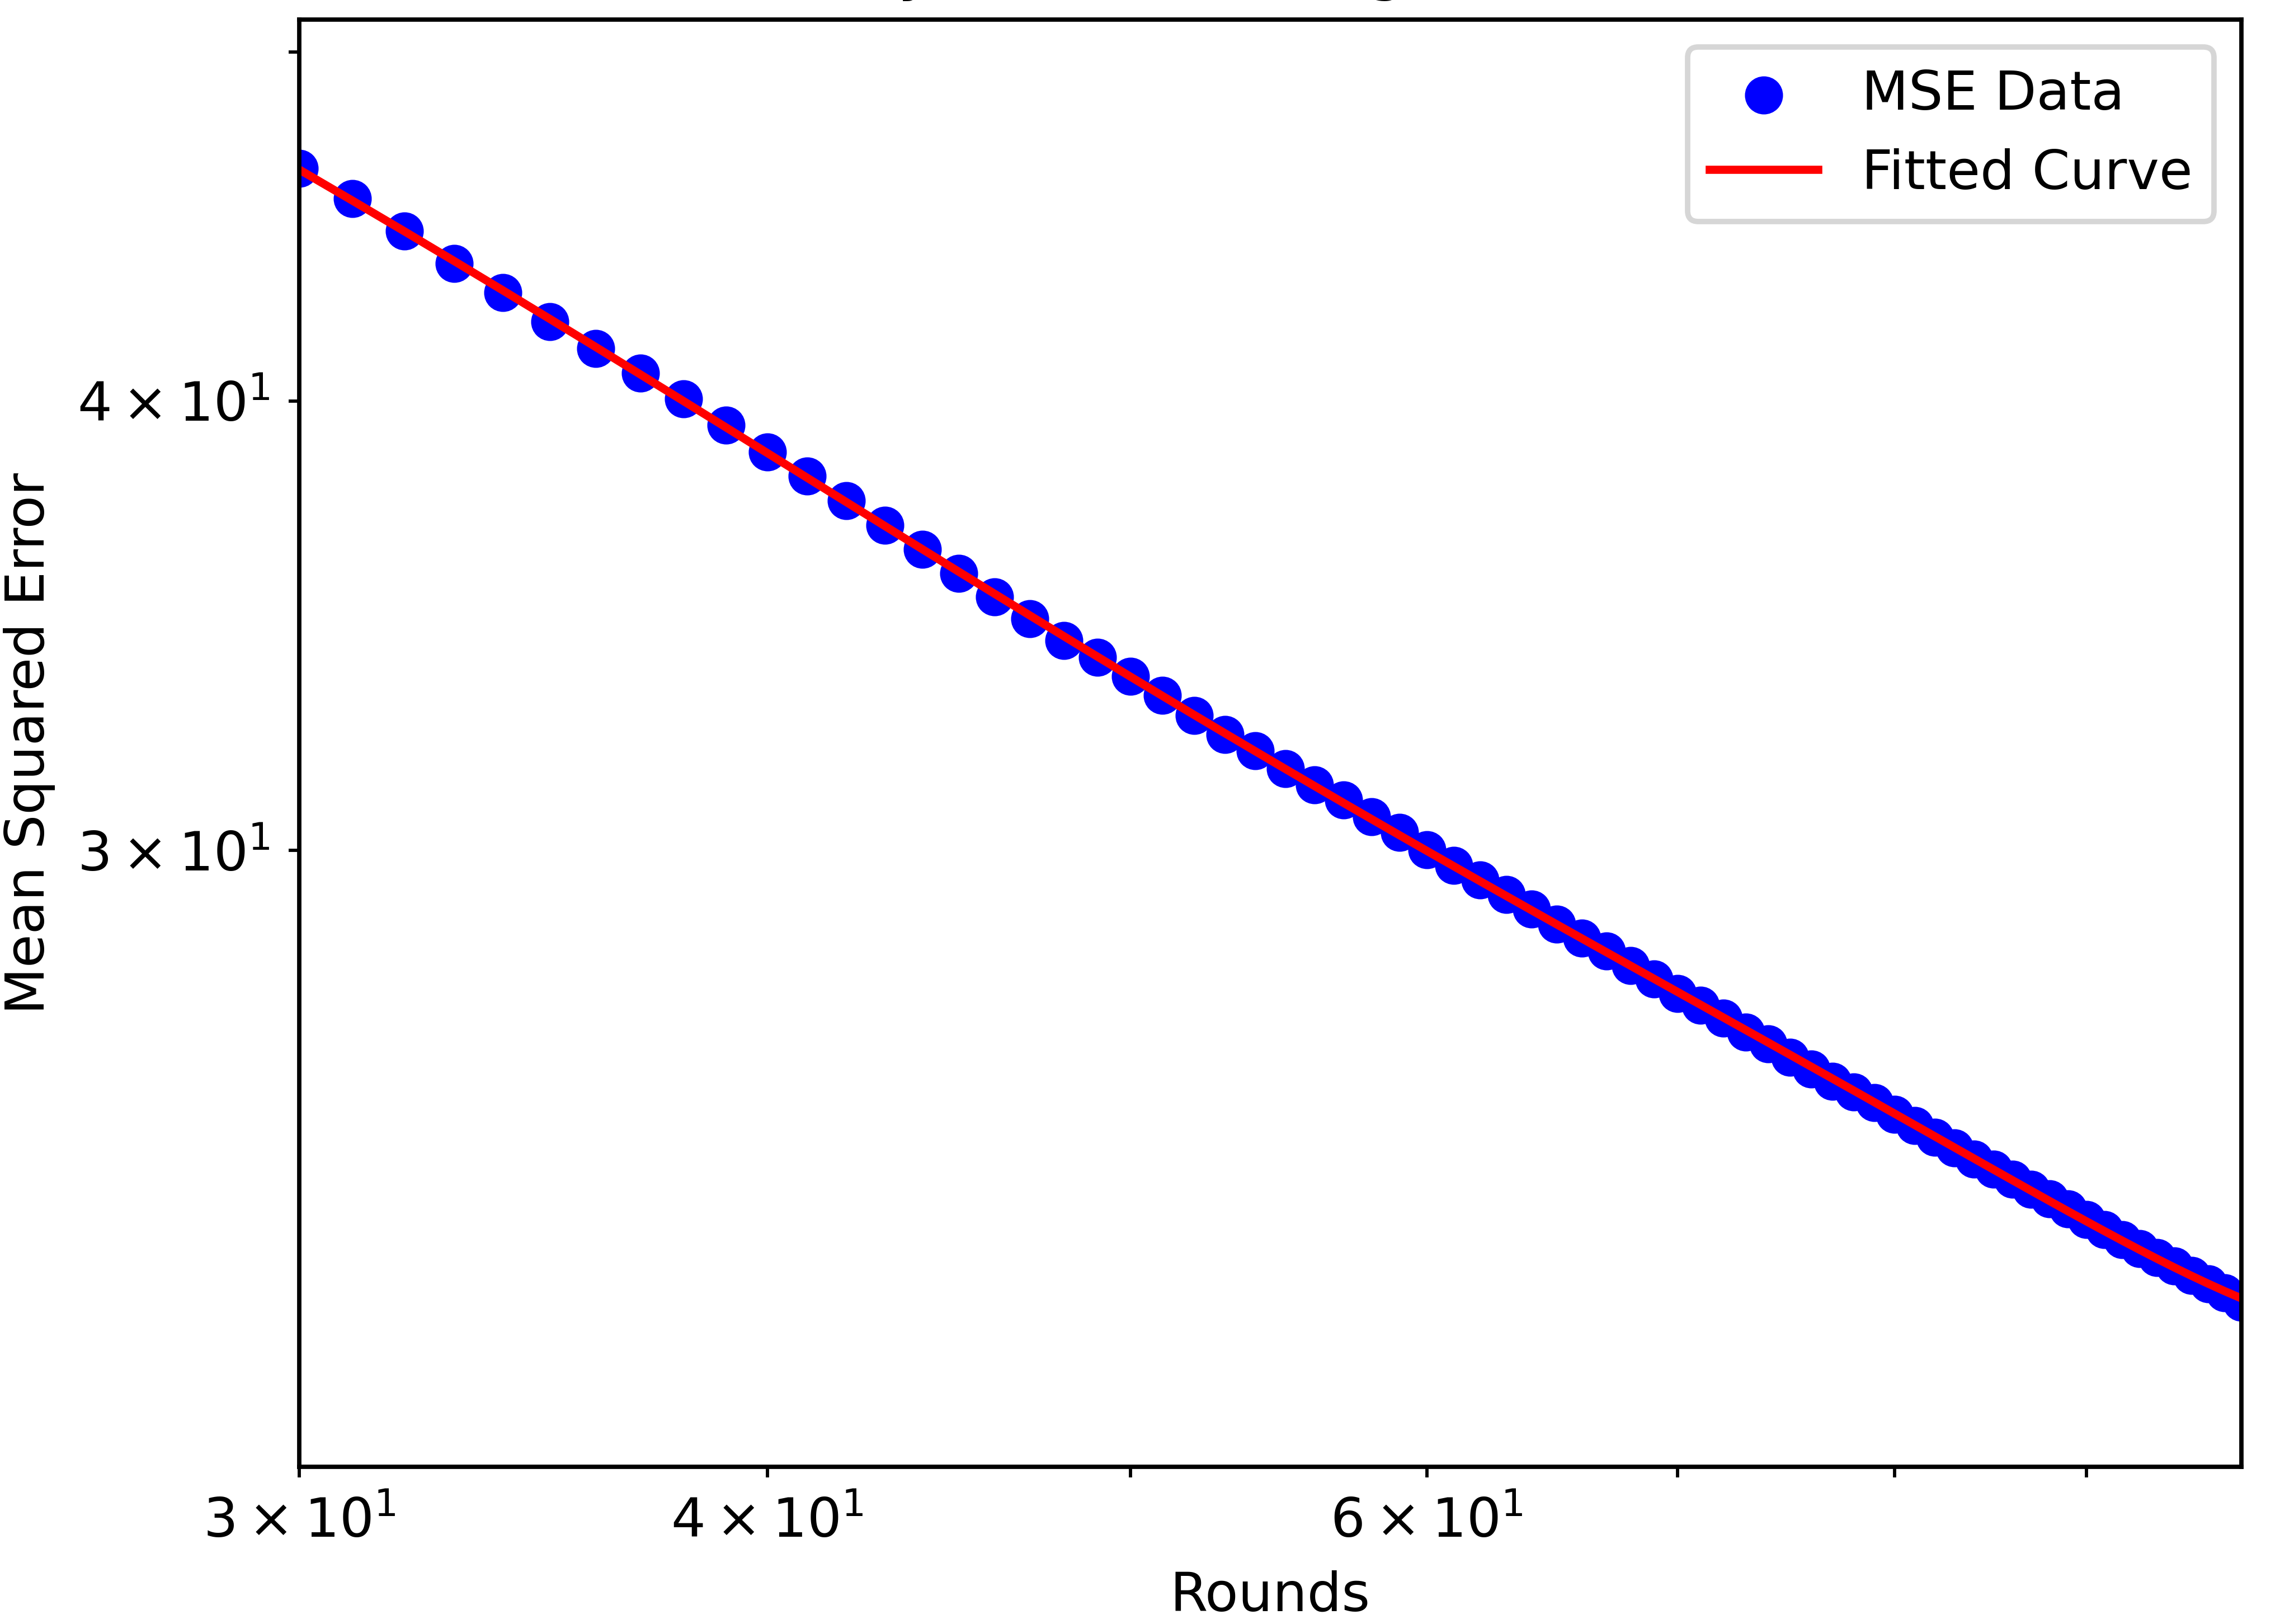
\includegraphics{figures/Simulation_outcomes/RingOfCliques/128x8/PPS/PPS_modelfitting_rounds_99_model_2.png}}
    \caption{$(128\times8)$-Ring of Cliques - polynomial regression fit: PPS}
    \label{fig:128x8ppsRingOfCliquesModelFit}
\end{figure}

\begin{figure}[]
    \centering
    \scalebox{0.8}{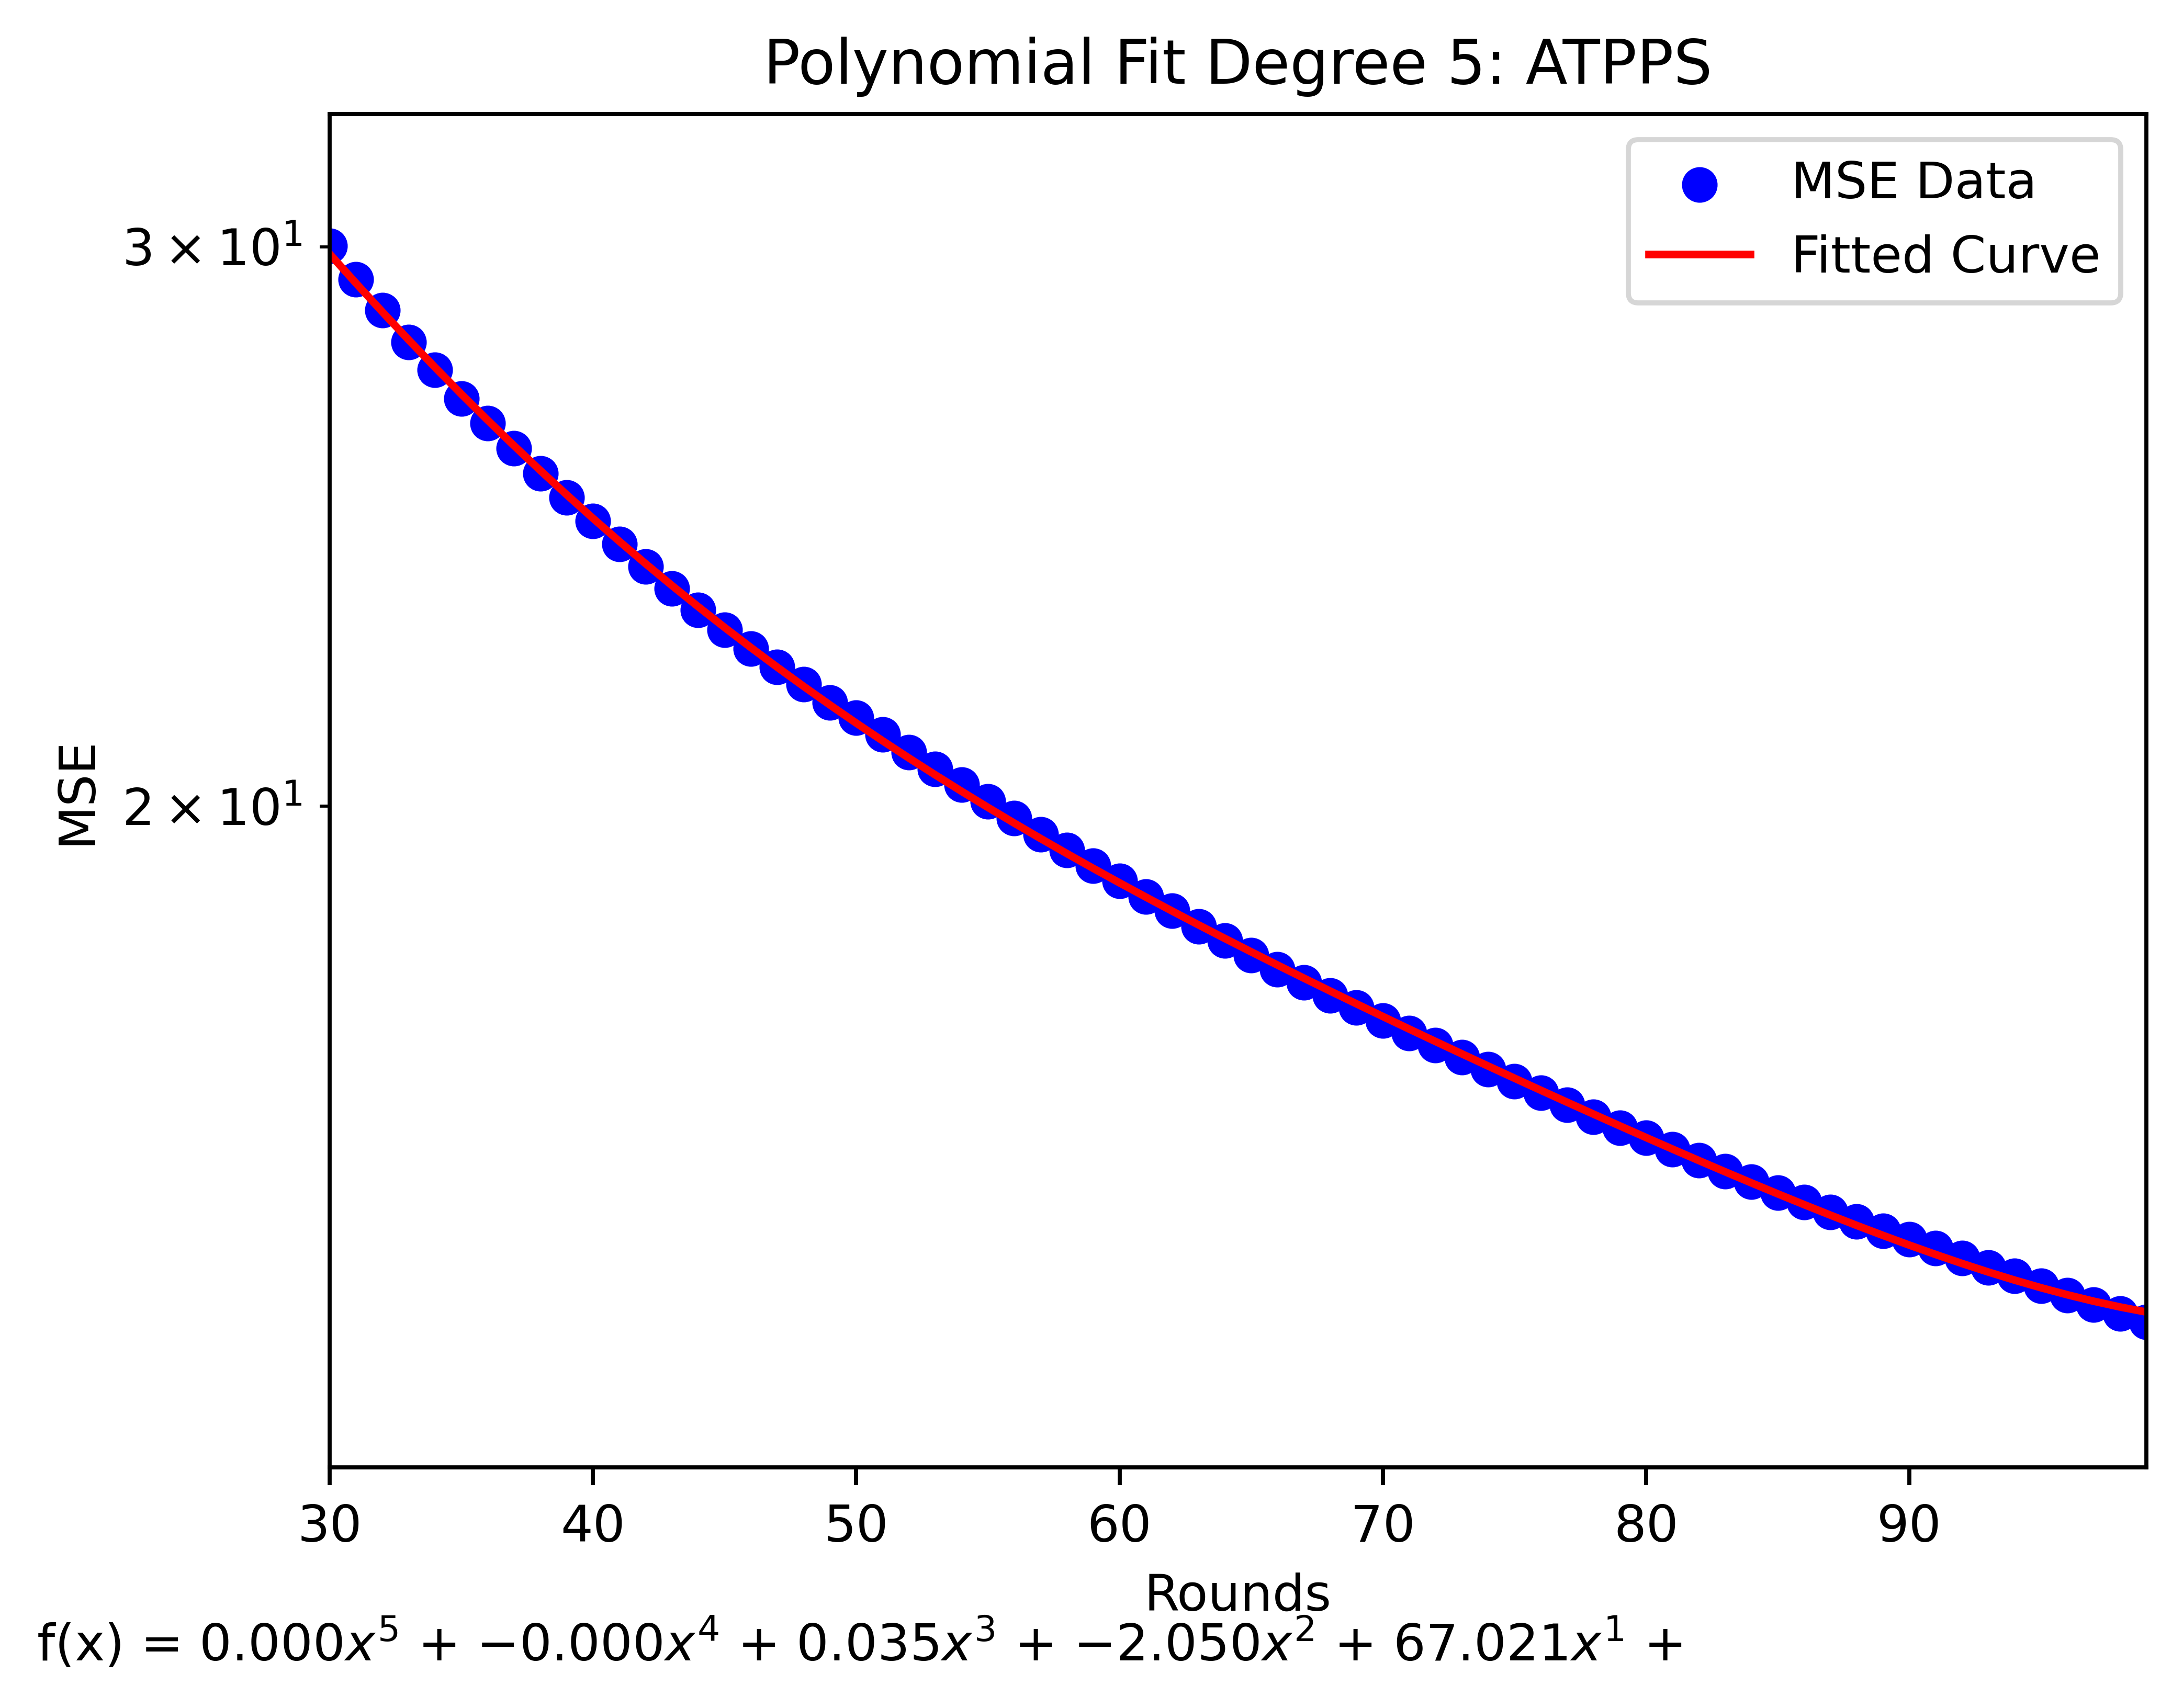
\includegraphics{figures/Simulation_outcomes/RingOfCliques/128x8/ATPPS/ATPPS_modelfitting_rounds_99_model_2.png}}
    \caption{$(128\times8)$-Ring of Cliques - polynomial regression fit: ATPPS}
    \label{fig:128x8atppsRingOfCliquesModelFit}
\end{figure}

\begin{figure}
    \centering
    \scalebox{0.8}{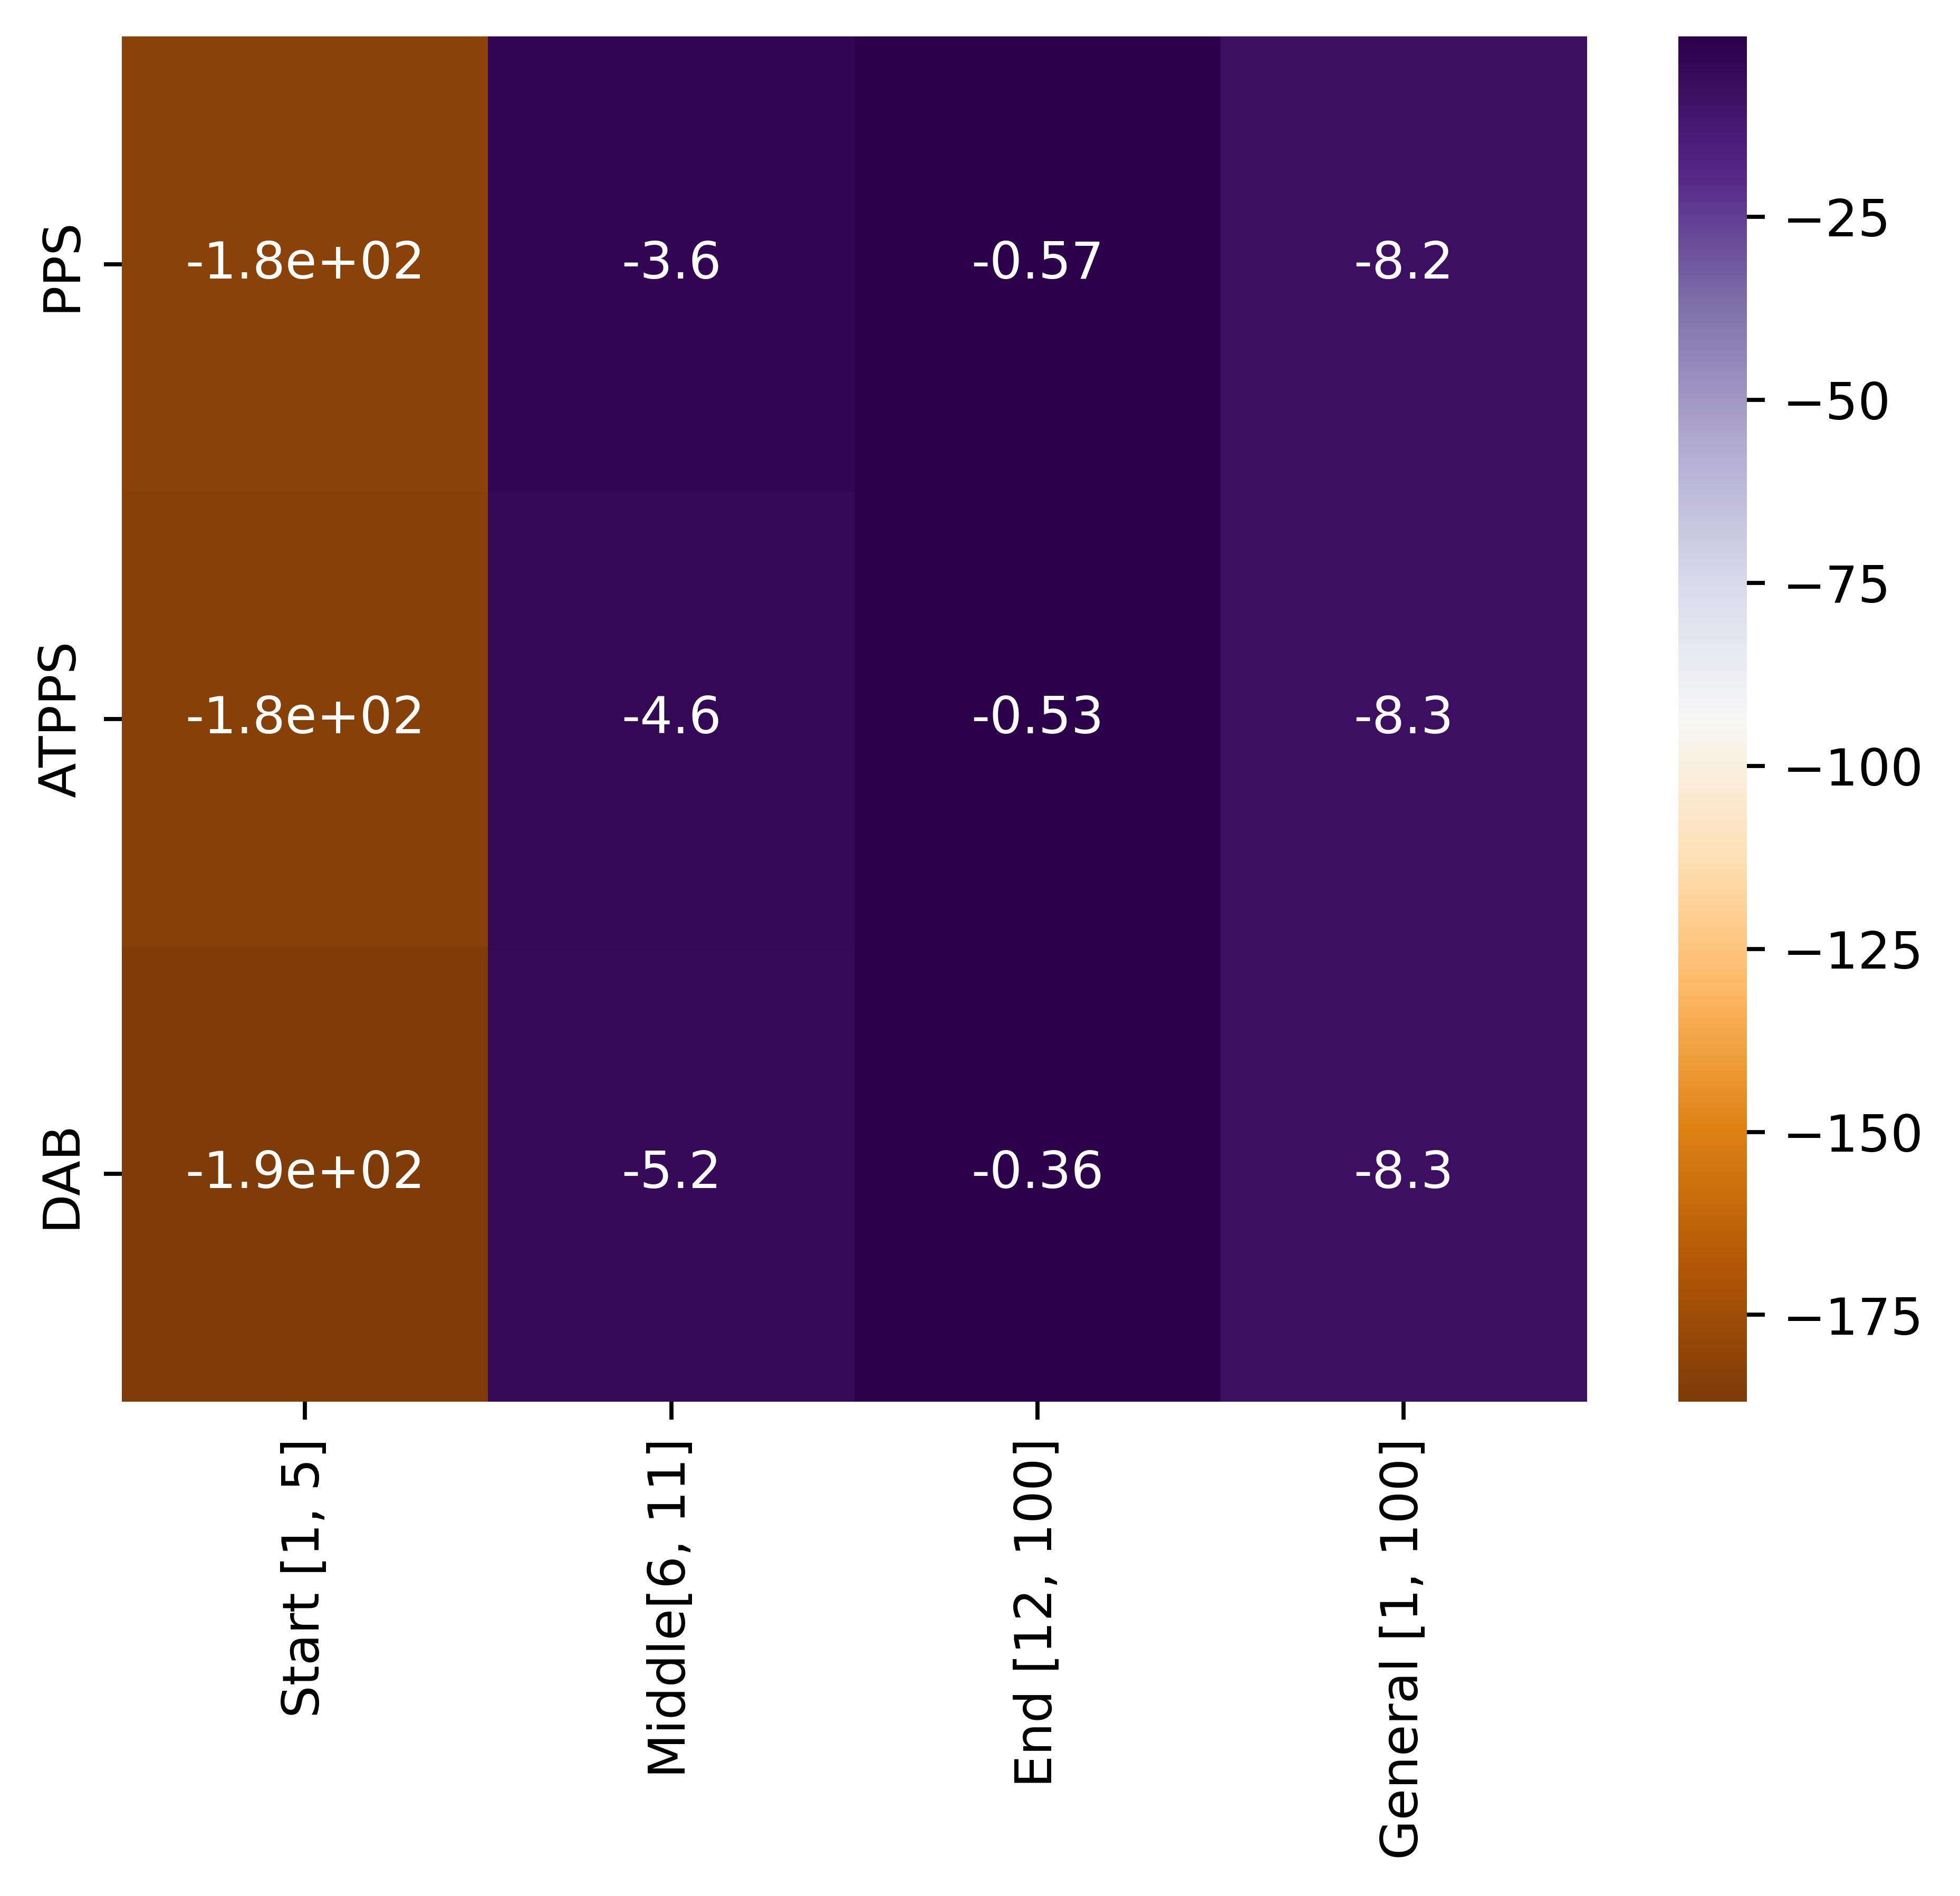
\includegraphics{figures/Simulation_outcomes/RingOfCliques/128x8/DAB_vs_PPS_vs_ATPPS_slopesheatmap_100rounds.png}}
    \caption{$(128\times8)$-Ring of Cliques: heat map of slopes per region}
    \label{fig:128x8ringOfCliquesslopes}
\end{figure}

\subsection{8x128 Ring of Cliques}\label{subsec:8_128ROC}
Increasing the clique size and reducing the number of cliques favors the Push-Pull Sum based algorithms, which show a very steep decrease of error in the first 5 rounds of the simulation. The error is reduced by -200 on average in this region for each Push-Pull Sum based algorithm. The DAB data shows a more moderate decrease by -36 in this region. The error reduction reduces over the next regions, since the error of the network is already very low and the network is in a state of good balance showing a MSE in this region of around $\sim -30$ for the Push-Pull Sum based algorithms. After the first region the state of the network managed by the DAB is still very unbalanced and thus the balance potential is higher. This is shown by the slopes in the middle region. The Push-Pull Sum based algorithms reduce the error by $\sim -2$ while the DAB shows a still very high value of $\sim -30$. The reason behind this behavior is due to the impact of the clique sizes. The Push-Pull Sum based algorithms achieve good performances in reducing error in this scenario compared to the DAB which struggles in the context of dense graphs. The steep decrease and the low MSE values after rounds 5 and 10 stem from the fast error reduction in the cliques while still having to spread loads from clique to clique through the briding nodes. Compared to the experiment in the $(8 \times 128)$-Ring of Cliques in \ref{subsec:128_8ROC} the error after rounds 100 drop to lower values. After rounds 100 the DAB achieves a MSE value of 5.18 compared to 5.95 for the PPS and 4.56 for the ATPPS. especially in the last region (rounds 12 to 100) the DAB catches up to the PPS-based algorithms. However, the Push-Pull Sum based algorithms achieved a broadly balanaced state of the network after round 10 dropping the error to a MSE value of 7. In the following rounds the inter -clique error reduction follows. Here the PPS algorithm has difficulties, since the algorithms orders the nodes of the network to choose their transfer partner by random. The ATPPS has an advantage compared to the PPS here since it prioritizes the bridging nodes once its neighbors within the clique are already balanced. This elaborates why the PPS curve is mostly stagnating, while the ATPPS curve shows a downwards trend. The stagnating trend between rounds 20 to 100 is expressed by the linear mode fit in figure \ref{fig:8x128ppsRingOfCliquesModelFit}. The best-fit model follows the equation. $MSE_r=-0.0015x+6.05$. The PPS curve shows a complexer relation between the MSE reduction over the rounds, namely a polynomial of degree 2 following the equation $MSE_r=6.07\times 10^{-5}r^{2}-0.02r+6.39$ (figure \ref{fig:8x128ppsRingOfCliquesModelFit}). The DAB does not follow a single power relation ship in this region. Between the rounds 15 to 50 the error reduction can be expressed by a third degree polynomial $MSE_r=-3.33\times 10^{-3}r^{3}+0.63r^{2}-40.23r+872.75$ (figure \ref{fig:8x128atppsRingOfCliquesModelFit} a)) while in later rounds the power relation is a bit complexer, expressed by a fourth degree polynomial following the equation $MSE_r=2.96 \times 10^{-6}r^{4}-9.97\times 10^{-3}r^{3}+0.13r^{2}-7.16r+161.73$ (figure \ref{fig:8x128atppsRingOfCliquesModelFit} b)).

Snippets of the simulation outcomes after the 100th rounds of each load balancing algorithm verify that within the cliques the load is balanced, however the inter clique connection seems to be pending. Listing \ref{lst:exampleROCOutcomes} shows the simulation outcomes of two connected cliques balanced by the ATPPS in round 100. While the first clique converged to a value of $\sim 46.35$ the second clique averaged to $\sim 47.90$. The ground truth of the first clique is $45.89$ and the ground truth of the second clique is $48.13$. So the simulation outcomes and the ground truths align, however the averages do not align with the ground truth of the Ring of Cliques (which is $49.09$) itself. The PPS simulation outcomes show a similiar behavior.
\begin{figure}[!ht]
    \centering
        \subfloat[]{\includegraphics[width=0.49\linewidth]{figures/Simulation_outcomes/RingOfCliques/8x128/DAB_vs_PPS_RoC_r100_n1024_averaged_log.png}}
    \hfil
        \subfloat[]{\includegraphics[width=0.49\linewidth]{figures/Simulation_outcomes/RingOfCliques/8x128/DAB_vs_PPS_RoC_r100_n1024_averaged_loglog.png}}
    \caption{$(8\times128)$-Ring of Cliques: mean squared error per rounds (log-linear and log-log)}
        \label{fig:128x8RingOfCliquesLog_LogLog}
\end{figure}

\begin{figure}[!ht]
    \centering
        \subfloat[]{\includegraphics[width=0.49\linewidth]{figures/Simulation_outcomes/RingOfCliques/8x128/DAB/DAB_modelfitting_rounds_49_model_2.png}}
    \hfil
        \subfloat[]{\includegraphics[width=0.49\linewidth]{figures/Simulation_outcomes/RingOfCliques/8x128/DAB/DAB_modelfitting_rounds_99_model_2.png}}
    \caption{$(8\times128)$-Ring of Cliques - polynomial regression fit: rounds 20-50 and 55-100}
        \label{fig:8x128dabRingOfCliquesModelFit}
\end{figure}
\begin{figure}[]
    \centering
    \scalebox{0.8}{\includegraphics{figures/Simulation_outcomes/RingOfCliques/8x128/PPS/PPS_modelfitting_rounds_99_model_0.png}}
    \caption{$(8\times128)$-Ring of Cliques - polynomial regression fit: PPS}
    \label{fig:8x128ppsRingOfCliquesModelFit}
\end{figure}

\begin{figure}[]
    \centering
    \scalebox{0.8}{\includegraphics{figures/Simulation_outcomes/RingOfCliques/8x128/ATPPS/ATPPS_modelfitting_rounds_99_model_2.png}}
    \caption{$(8\times128)$-Ring of Cliques - polynomial regression fit: ATPPS}
    \label{fig:8x128atppsRingOfCliquesModelFit}
\end{figure}

\begin{figure}
    \centering
    \scalebox{0.8}{\includegraphics{figures/Simulation_outcomes/RingOfCliques/8x128/DAB_vs_PPS_vs_ATPPS_slopesheatmap_100rounds.png}}
    \caption{$(8\times128)$-Ring of Cliques: heat map of slopes per region}
    \label{fig:128x8ringOfCliquesslopes}
\end{figure}

\begin{lstlisting}[caption=Snippet of simulation outcomes ATPPS: Experiment 2, captionpos=b, label=lst:exampleROCOutcomes]
# First Clique starts here
ID 0	 sum 23.703116631927735	 weight 0.5112902995975737	 Average 46.359410007551446
ID 1	 sum 39.52476483621201	 weight 0.852801600538612	 Average 46.34696371494727
ID 2	 sum 8.793798989811481	 weight 0.18958634077240344	 Average 46.38413798158778
...
ID 125	 sum 94.3005473042508	 weight 2.0354736681273184	 Average 46.32855181615266
ID 126	 sum 145.10578299145917	 weight 3.1321941681390815	 Average 46.32719914604474
ID 127	 sum 149.43516229432458	 weight 3.222997634840688	 Average 46.365272092950555
# First Cliques ends here

# Second Clique starts here
ID 128	 sum 198.97437468622982	 weight 4.149869252421544	 Average 47.947143050380134
ID 129	 sum 168.24642313171216	 weight 3.5107838866374186	 Average 47.92275131832632
ID 130	 sum 35.6266112221637	 weight 0.7449330697151406	 Average 47.82525124812511
...
ID 253	 sum 63.87360335784297	 weight 1.3317373880292274	 Average 47.962611797185005
ID 254	 sum 15.173810743452982	 weight 0.31637895519911763	 Average 47.96087253623784
ID 255	 sum 19.982619800226413	 weight 0.4175626540105257	 Average 47.85538076334456
# Second Cliques ends here
\end{lstlisting}